\documentclass[letterpaper, 11pt, notitlepage]{report}

% --- Main packages ---

\usepackage[dvipsnames]{xcolor} % Extended set of colors

\usepackage{
  amsmath, amsthm, amssymb, mathtools, dsfont, units, % Math typesetting
  graphicx, wrapfig, subfig, float, % Figures and graphics formatting
  listings, color, inconsolata, pythonhighlight, % Code formatting
  fancyhdr, sectsty, hyperref, enumerate, enumitem, framed } % Headers/footers, section fonts, links, lists

\usepackage{hyperref} 

\usepackage{newpxtext, newpxmath, inconsolata} % Fonts

% --- Page layout settings ---

% Set page margins
\usepackage[left=1.35in, right=1.35in, top=1.0in, bottom=.9in, headsep=.2in, footskip=0.35in]{geometry}

% Anchor footnotes to the bottom of the page
\usepackage[bottom]{footmisc}

% Set line spacing
\renewcommand{\baselinestretch}{1.2}

% Set spacing between paragraphs
\setlength{\parskip}{1.3mm}

% Allow multi-line equations to break onto the next page
\allowdisplaybreaks

% --- Page formatting settings ---

% Set image captions to be italicized
\usepackage[font={it,footnotesize}]{caption}

% Set link colors for labeled items (blue), citations (red), URLs (orange)
\hypersetup{colorlinks=true, linkcolor=RoyalBlue, citecolor=RedOrange, urlcolor=ForestGreen}

% Set font size for section titles (\large) and subtitles (\normalsize) 
\usepackage{titlesec}
\usepackage{adforn}

\definecolor{gray75}{gray}{0.75}
\newcommand{\hsp}{\hspace{10pt}}

\titleformat{\chapter}{\LARGE\bfseries}{{\fontsize{22}{0}\selectfont\thechapter\hsp\textcolor{gray75}{|}\hsp}\;\;}{0em}{}
\titleformat{\section}{\Large\bfseries}{{\fontsize{15}{0}\selectfont\thesection}\;\;}{0em}{}
\titleformat{\subsection}{\normalsize\bfseries\selectfont}{{\fontsize{12}{16}\selectfont\adfoutlineleafright}\;\;}{0em}{}

% Enumerated/bulleted lists: make numbers/bullets flush left
%\setlist[enumerate]{wide=2pt, leftmargin=16pt, labelwidth=0pt}
\setlist[itemize]{wide=0pt, leftmargin=16pt, labelwidth=10pt, align=left}

% --- Table of contents settings ---

\setcounter{tocdepth}{1} 
\usepackage[subfigure]{tocloft}

% Reduce spacing between sections in table of contents
\setlength{\cftbeforesecskip}{.9ex}

% Remove indentation for sections
\cftsetindents{chapter}{0em}{0em}
\cftsetindents{section}{0em}{0em}

% Set font size (\large) for table of contents title
\renewcommand{\cfttoctitlefont}{\large\bfseries}

% Remove numbers/bullets from section titles in table of contents
\makeatletter
\renewcommand{\cftsecpresnum}{\begin{lrbox}{\@tempboxa}}
\renewcommand{\cftsecaftersnum}{\end{lrbox}}
\makeatother

\makeatletter
\renewcommand{\cftchappresnum}{\begin{lrbox}{\@tempboxa}}
\renewcommand{\cftchapaftersnum}{\end{lrbox}}
\makeatother

% --- Math/Statistics commands ---

% Add a reference number to a single line of a multi-line equation
% Usage: "\numberthis\label{labelNameHere}" in an align or gather environment
\newcommand\numberthis{\addtocounter{equation}{1}\tag{\theequation}}

% Shortcut for bold text in math mode, e.g. $\b{X}$
\let\b\mathbf

% Shortcut for bold Greek letters, e.g. $\bg{\beta}$
\let\bg\boldsymbol

% Shortcut for calligraphic script, e.g. %\mc{M}$
\let\mc\mathcal

% --- Left/right header text (to appear on every page) ---

% Do not include a line under header or above footer
\pagestyle{fancy}
\renewcommand{\footrulewidth}{0pt}
\renewcommand{\headrulewidth}{0pt}

% Right header text: Lecture number and title
\renewcommand{\sectionmark}[1]{\markright{#1} }
\fancyhead[R]{\small\textit{\nouppercase{\rightmark}}}

% Left header text: Short course title, hyperlinked to table of contents
\fancyhead[L]{\hyperref[sec:contents]{\small HE-AP Th}}

% Add bibliography to TOC
\usepackage[nottoc,numbib]{tocbibind}

\usepackage{amsmath,amsthm,amsfonts,amssymb,amscd}
\usepackage{aas_macros}
\usepackage{booktabs}
%\usepackage{calc}
\usepackage{cancel}
%\usepackage{empheq}
%\usepackage{enumitem}
%\usepackage{fancyhdr}
%\usepackage{framed}
%\usepackage{fullpage}
%\usepackage[margin=3cm]{geometry}
%\usepackage[utf8]{inputenc}
%\usepackage{lastpage}
%\usepackage{mathabx}
%\usepackage{mathrsfs}
%\usepackage{mdframed}
%\usepackage{multicol}
%\usepackage{multirow}
\usepackage{physics}
%\usepackage{setspace}
%\usepackage[most]{tcolorbox}
%\usepackage{todonotes}
%\usepackage{wrapfig}
%%\usepackage[table]{xcolor}
%
%\newlength{\tabcont}
\setlength{\parindent}{0.0in}
\setlength{\parskip}{0.05in}
%\colorlet{shadecolor}{orange!15}
%\parindent 0in
%\parskip 12pt
%\geometry{margin=1in, headsep=0.25in}
%
%\theoremstyle{definition}
%\newtheorem{defn}{Definition}
%\newtheorem{reg}{Rule}
%\newtheorem{exer}{Exercise}
%\newtheorem{note}{Note}
%\newtheorem{tbd}{Demonstration}
%
%\linespread{1.1}
%
%\usepackage{sectsty}
%\sectionfont{\large}
%
%\usepackage{hyperref}
%\hypersetup{
%    colorlinks,
%    citecolor=red,
%    filecolor=red,
%    linkcolor=blue,
%    urlcolor=red
%}

\newcommand\drsh{\rotatebox[origin=c]{180}{$\Lsh$}}

\DeclareRobustCommand{\rchi}{{\mathpalette\irchi\relax}}
\newcommand{\irchi}[2]{\raisebox{\depth}{$#1\chi$}} 

% theorems
\makeatother
\usepackage{thmtools}
\usepackage[framemethod=TikZ]{mdframed}
\mdfsetup{skipabove=1em,skipbelow=0em}

\theoremstyle{definition}

%\declaretheoremstyle[
%    headfont=\bfseries\sffamily\color{ForestGreen!70!black}, bodyfont=\normalfont,
%    mdframed={
%        linewidth=2pt,
%        rightline=false, topline=false, bottomline=false,
%        linecolor=ForestGreen, backgroundcolor=ForestGreen!5,
%    }
%]{thmgreenbox}

\declaretheoremstyle[
    headfont=\bfseries\sffamily\color{NavyBlue!70!black}, bodyfont=\normalfont,
    mdframed={
        linewidth=2pt,
        rightline=false, topline=false, bottomline=false,
        linecolor=NavyBlue, backgroundcolor=NavyBlue!5,
    }
]{thmbluebox}

\declaretheoremstyle[
    headfont=\bfseries\sffamily\color{NavyBlue!70!black}, bodyfont=\normalfont,
    mdframed={
        linewidth=2pt,
        rightline=false, topline=false, bottomline=false,
        linecolor=NavyBlue
    }
]{thmblueline}

%\declaretheoremstyle[
%    headfont=\bfseries\sffamily\color{RawSienna!70!black}, bodyfont=\normalfont,
%    mdframed={
%        linewidth=2pt,
%        rightline=false, topline=false, bottomline=false,
%        linecolor=RawSienna, backgroundcolor=RawSienna!5,
%    }
%]{thmredbox}
%
%\declaretheoremstyle[
%    headfont=\bfseries\sffamily\color{RawSienna!70!black}, bodyfont=\normalfont,
%    numbered=no,
%    mdframed={
%        linewidth=2pt,
%        rightline=false, topline=false, bottomline=false,
%        linecolor=RawSienna, backgroundcolor=RawSienna!1,
%    },
%    qed=\qedsymbol
%]{thmproofbox}
%
%\declaretheoremstyle[
%    headfont=\bfseries\sffamily\color{NavyBlue!70!black}, bodyfont=\normalfont,
%    numbered=no,
%    mdframed={
%        linewidth=2pt,
%        rightline=false, topline=false, bottomline=false,
%        linecolor=NavyBlue, backgroundcolor=NavyBlue!1,
%    },
%]{thmexplanationbox}

%\declaretheorem[style=thmgreenbox, name=Definition]{definition}
\declaretheorem[style=thmbluebox, numbered=no, name=Problem]{problem}
%\declaretheorem[style=thmredbox, name=Proposition]{prop}
%\declaretheorem[style=thmredbox, name=Theorem]{theorem}
%\declaretheorem[style=thmredbox, name=Lemma]{lemma}
%\declaretheorem[style=thmredbox, numbered=no, name=Corollary]{corollary}

%\declaretheorem[style=thmproofbox, name=Proof]{replacementproof}
%\renewenvironment{proof}[1][\proofname]{\vspace{-10pt}\begin{replacementproof}}{\end{replacementproof}}

%\declaretheorem[style=thmexplanationbox, name=Proof]{tmpexplanation}
%\newenvironment{explanation}[1][]{\vspace{-10pt}\begin{tmpexplanation}}{\end{tmpexplanation}}
%\declaretheorem[style=thmredbox, numbered=no]{remark}

\newmdenv[  
topline=false,  
rightline=false,  
bottomline=false,  
leftline=true,  
linecolor=RawSienna!95!black,  
linewidth=3pt,  
backgroundcolor=RawSienna!10,  
]{remark} 

\declaretheorem[style=thmblueline, numbered=no, name=Note]{note}

% new \oset macro:
\makeatletter
\newcommand{\oset}[3][1.4ex]{%
  \mathrel{\mathop{#3}\limits^{
    \vbox to#1{\kern-2\ex@
    \hbox{$\scriptstyle#2$}\vss}}}}
\makeatother

%\newtheorem*{uovt}{UOVT}
%\newtheorem*{notation}{Notation}
%\newtheorem*{previouslyseen}{As previously seen}
%\newtheorem*{problem}{Problem}
%\newtheorem*{observe}{Observe}
%\newtheorem*{property}{Property}
%\newtheorem*{intuition}{Intuition}

\newcommand{\TODO}[1]{{\color{yellow!70!black}[#1]}}

\graphicspath{{figures/}{../figures/}}

\begin{document}

\title{High-Energy Astroparticle Theory \\[1em]
\normalsize A.Y.~2024/25}

\author{\normalsize Carmelo Evoli}
\date{\normalsize\vspace{-1ex} Last updated: \today}

\maketitle

\vspace{0.25cm}
{\color{red}\large This document is currently under active development. The content is subject to change as revisions are ongoing. I expect to release a stable and comprehensive version no earlier than January 2026.}
\vspace{0.25cm}

These lecture notes are largely based on:
%
\begin{itemize}
\item P.~Blasi, \emph{The origin of galactic cosmic rays}, A\&AR, 21, 70, 2013, \href{https://arxiv.org/abs/1311.7346}{arXiv:1311.7346}
\item P.D.~Serpico, \emph{Cosmic ray interactions with matter and radiation}, Proceedings of the International School of Physics ``Enrico Fermi'', Course 208, Varenna 2022, \href{https://arxiv.org/abs/2308.04361}{arXiv:2308.04361}
\item D.~Boncioli, \emph{Cosmic-ray propagation in extragalactic space and secondary messengers}, Proceedings of the International School of Physics ``Enrico Fermi'', Course 208, Varenna 2022, \href{https://arxiv.org/abs/2309.12743}{arXiv:2309.12743}
\item C.~Evoli \& U.~Dupletsa, \emph{Phenomenological models of Cosmic Ray transport in Galaxies}, Proceedings of the International School of Physics ``Enrico Fermi'', Course 208, Varenna 2022, \href{https://arxiv.org/abs/2309.00298}{arXiv:2309.00298}
\end{itemize}

Useful readings:
%
\begin{itemize}
\item M.~Vietri, \emph{Foundations of High-Energy Astrophysics}, April 2008, U.~Chicago Press
\item R.~Blandford \& D.~Eichler, \emph{Particle acceleration at astrophysical shocks: A theory of cosmic ray origin},  October 1987, Physics Reports, 154
\item G.B.~Rybicki \& A.P.~Lightman, \emph{Radiative Processes in Astrophysics}, May 1985, Vch Pub
\item T.K.~Gaisser, R.~Engel \& E.~Resconi, \emph{Cosmic Rays and Particle Physics}, June 2016, Cambridge University Press
\item D.~Overbye, \emph{Lonely Hearts of the Cosmos: The Story of the Scientific Quest for the Secret of the Universe}, November 1999, Back Bay Books
\end{itemize}

\newpage

\tableofcontents\label{sec:contents}

\chapter{Radiative Processes in Astroparticle Physics}
% !TEX root = ../lectures.tex
\section{The Multi-Messenger View of Astroparticle Physics}

The investigation of secondary messengers emitted by high-energy particles and their absorption in space plays a crucial role in astroparticle physics, shedding light on diverse cosmic phenomena. 

A key aspect of radiative processes is their influence on the energy spectrum of high-energy events. Interactions between particles, electromagnetic fields, and matter, involving mechanisms like synchrotron radiation, bremsstrahlung, and inverse Compton scattering, can lead to significant energy losses. These losses modify the energy distribution of particles, affecting the spectrum observed from these high-energy sources.

Furthermore, secondary emissions serve as powerful diagnostic tools for understanding the physical properties and behaviors of astrophysical systems, even when the radiative process is subdominant. 
%
For instance, the Galaxy's diffuse gamma-ray emission offers crucial information about cosmic ray densities, sources, and propagation, although the emission of these photons is due to a process, pion production, which is sub-leading when describing the transport of protons in the ISM.

% !TEX root = ../lectures.tex
\section{Synchrotron Radiation}

Synchrotron radiation, denoted by the process \( e + B \rightarrow e + \gamma + B \), is emitted by relativistic charged particles as they undergo acceleration in a static magnetic field. In the non-relativistic regime, this is known as 
\textbf{cyclotron emission}.

Starting with the basic Larmor formula, the total power emitted by an accelerating or decelerating electron (or any charged particle) in c.g.s. units is:
%
\[
P = \frac{2}{3} q^2 \frac{a^2}{c^3}
\]
%
where \( a = \| \vb a \|\) is the acceleration.

The heuristic derivation of this formula includes: a) Radiative processes are proportional to \( q^2 \), as the cross-section \( \sigma \) is the square of the amplitude which for e.m. process is \( \propto q \), b) Consistency with relativity requires dependence only on acceleration, not velocity, since power is a relativistic invariant being the ratio of two time-like components, and c) Dimensional analysis justifies the \( a^2 \) term.

In relativistic scenarios, the Larmor formula is valid if \( a^2 \) is replaced by \( a^\mu a_\mu \), the invariant square of the four-acceleration. 

\begin{problem}
Demonstrate that \( a^\mu a_\mu \)  is a relativistic invariant.
\end{problem}

Considering the Lorentz force, the acceleration is perpendicular to velocity:
%
\[
\vb a = \frac{\vb F}{m} = \frac{\gamma q}{m} \left(\frac{\vb v}{c} \times \vb B \right)
\]
%
leading to:
%
\[
a^2 = \frac{q^2}{m^2} \frac{v_\perp^2}{c^2} \gamma^2 B^2 \longrightarrow a^2 = \frac{q^2}{m^2} \gamma^2 \beta^2 B^2 \sin^2 \theta
\]

The power emitted by synchrotron radiation in the limit \( \beta \rightarrow 1 \) is then:
%
\[
P_{\rm s} = \frac{2}{3} \frac{q^4 B^2}{m^2 c^3} \gamma^2 \sin^2 \theta
\]

Notably, synchrotron radiation is predominantly significant for leptons rather than nuclei, as \( P_{\rm s} \propto 1/m^4 \).

For an isotropic particle distribution, the average emitted power becomes:
%
\begin{remark}
\[
\langle P_{\rm s} \rangle = \frac{4}{9} \frac{q^4 B^2}{m^2 c^3} \gamma^2 = \frac{4}{3} c \sigma_{\rm T} \left(\frac{m_e}{m}\right)^2 \gamma^2 U_{\rm B}
\]
\end{remark}

using \( U_{\text{B}} = \frac{B^2}{8\pi} \) and \( \sigma_{\text{T}} = \frac{8\pi}{3} \left( \frac{q^2}{m_e c^2} \right)^2 \), and the average over the angle
%
\[
\langle \sin^2 \theta \rangle = \frac{1}{4\pi} \int d\Omega \sin^2 \theta = \frac{1}{4\pi} \int_0^{2\pi} \int_0^\pi \sin^2 \theta \sin \theta d\theta = \frac{2}{3}
\]

The electron energy loss timescale, important for understanding cooling rates, is:
%
\begin{remark}
\[
\tau_{\text{loss}} (\gamma) \simeq \frac{E}{| dE/dt |} = \frac{\gamma m_e c^2}{\langle P_s \rangle} = \frac{3}{4} \frac{m_e c}{\sigma_{\text{T}}} \frac{1}{\gamma U_{\text{B}}} \propto \frac{1}{E}
\]
\end{remark}
%
leading to the notable result that more energetic particles have shorter lifetimes.

\begin{problem}
The CRAB.
\end{problem}

To determine the emission spectrum of an electron with a specific energy, we consider the spectrum \( P_\nu \) as the frequency power spectrum of \( P(t) \), proportional to \( |a(t)|^2 \). To derive \( P_\nu \), we employ a Fourier transform, which translates the time-domain signal into its frequency components.

In synchrotron radiation, the effect of relativistic beaming is crucial. This phenomenon, combined with the fundamental gyromotion of electrons in a magnetic field, results in the emitted power being concentrated at frequencies much higher than the gyrofrequency \( \nu_g \) (see derivation in appendix).

Let's first derive the aberration formula, assuming the primed frame is seen from the unprimed frame as moving with speed $\beta = v/c$ along the x-axis:
%
\begin{eqnarray*}
c t^\prime & = & \gamma (c t - \beta x) \\
x^\prime & = & \gamma (x - \beta c t) \\
y^\prime & = & y 
\end{eqnarray*}

The velocity components transform as follows:
%
\begin{eqnarray*}
u_x & = & \frac{u'_x + \beta c}{1+\beta u'_x / c} \\
u_y & = & \frac{u'_y}{\gamma(1+\beta u'_x / c)} 
\end{eqnarray*}

Therefore, the emission angle \( \theta \) is given by:
%
\[
\tan \theta = \frac{u_y}{u_x} = \frac{u^\prime_y}{\gamma(u^\prime_x + \beta c)} = \frac{u^\prime \sin \theta^\prime}{\gamma(\beta c + u^\prime \cos \theta^\prime)} 
\]

For light (with \( u^\prime = c \)), the aberration formula becomes:
%
\begin{remark}
\[
\tan \theta = \frac{\sin \theta^\prime}{\gamma(\beta + \cos \theta^\prime)} 
\]
\end{remark}

\begin{figure}[t]
\centering
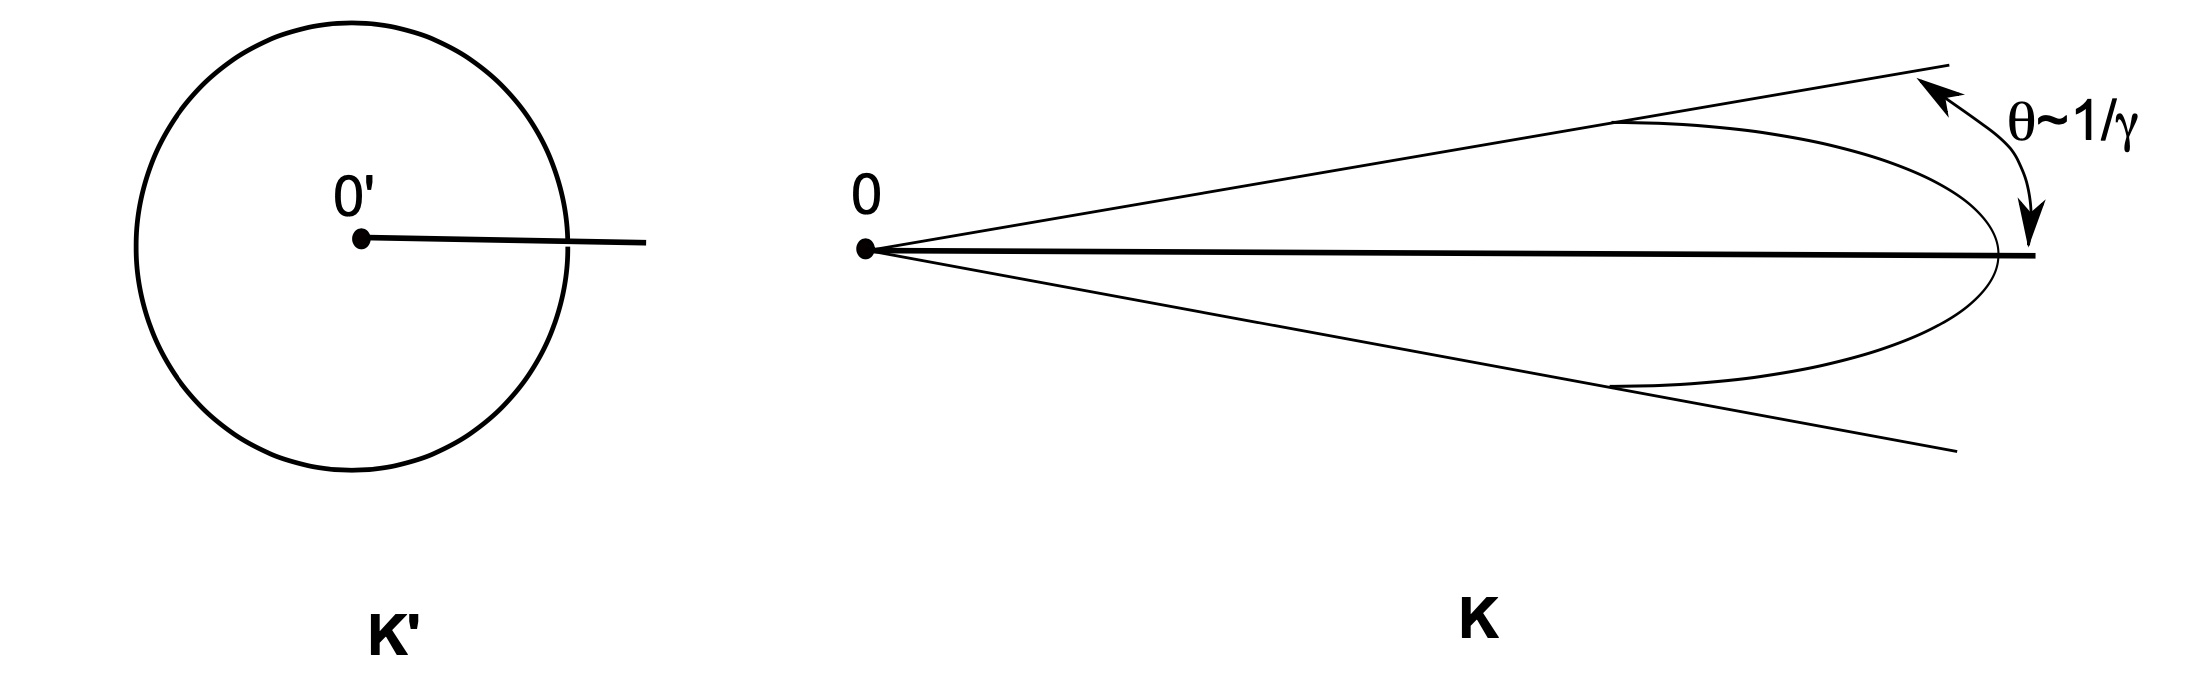
\includegraphics[width=0.8\textwidth]{aberration.jpg}
\caption{aberration}
\end{figure}

A photon emitted at \( \theta^\prime = 0 \) in the primed frame travels at \( \theta = 0 \) in the observer's frame. Conversely, a photon emitted at \( \theta^\prime = \frac{\pi}{2} \) travels at an angle \( \theta \) approximated by \( \theta \simeq \frac{1}{\gamma} \).

This indicates that emission isotropic at the source is not perceived as isotropic by an observer if there is a relativistic boost between them. This is particularly relevant for phenomena like gamma-ray bursts (GRBs), which are strongly beamed in the forward direction, forming a cone with an opening angle of approximately \( \sim \frac{2}{\gamma} \).

In the non-relativistic limit, the frequency of the emitted radiation corresponds to the gyro-frequency, leading to a mono-chromatic spectrum at this frequency.

However, in the relativistic regime, continuous emission is altered by the beaming effect. The signal is visible only at specific angles due to this effect. The resulting spectrum is still a Fourier transform of the time-dependent emission, but now it has a characteristic timescale \(  \Delta t \), giving a frequency spectrum peaked around \( \sim \frac{1}{\Delta t} \).

\begin{figure}[t]
\centering
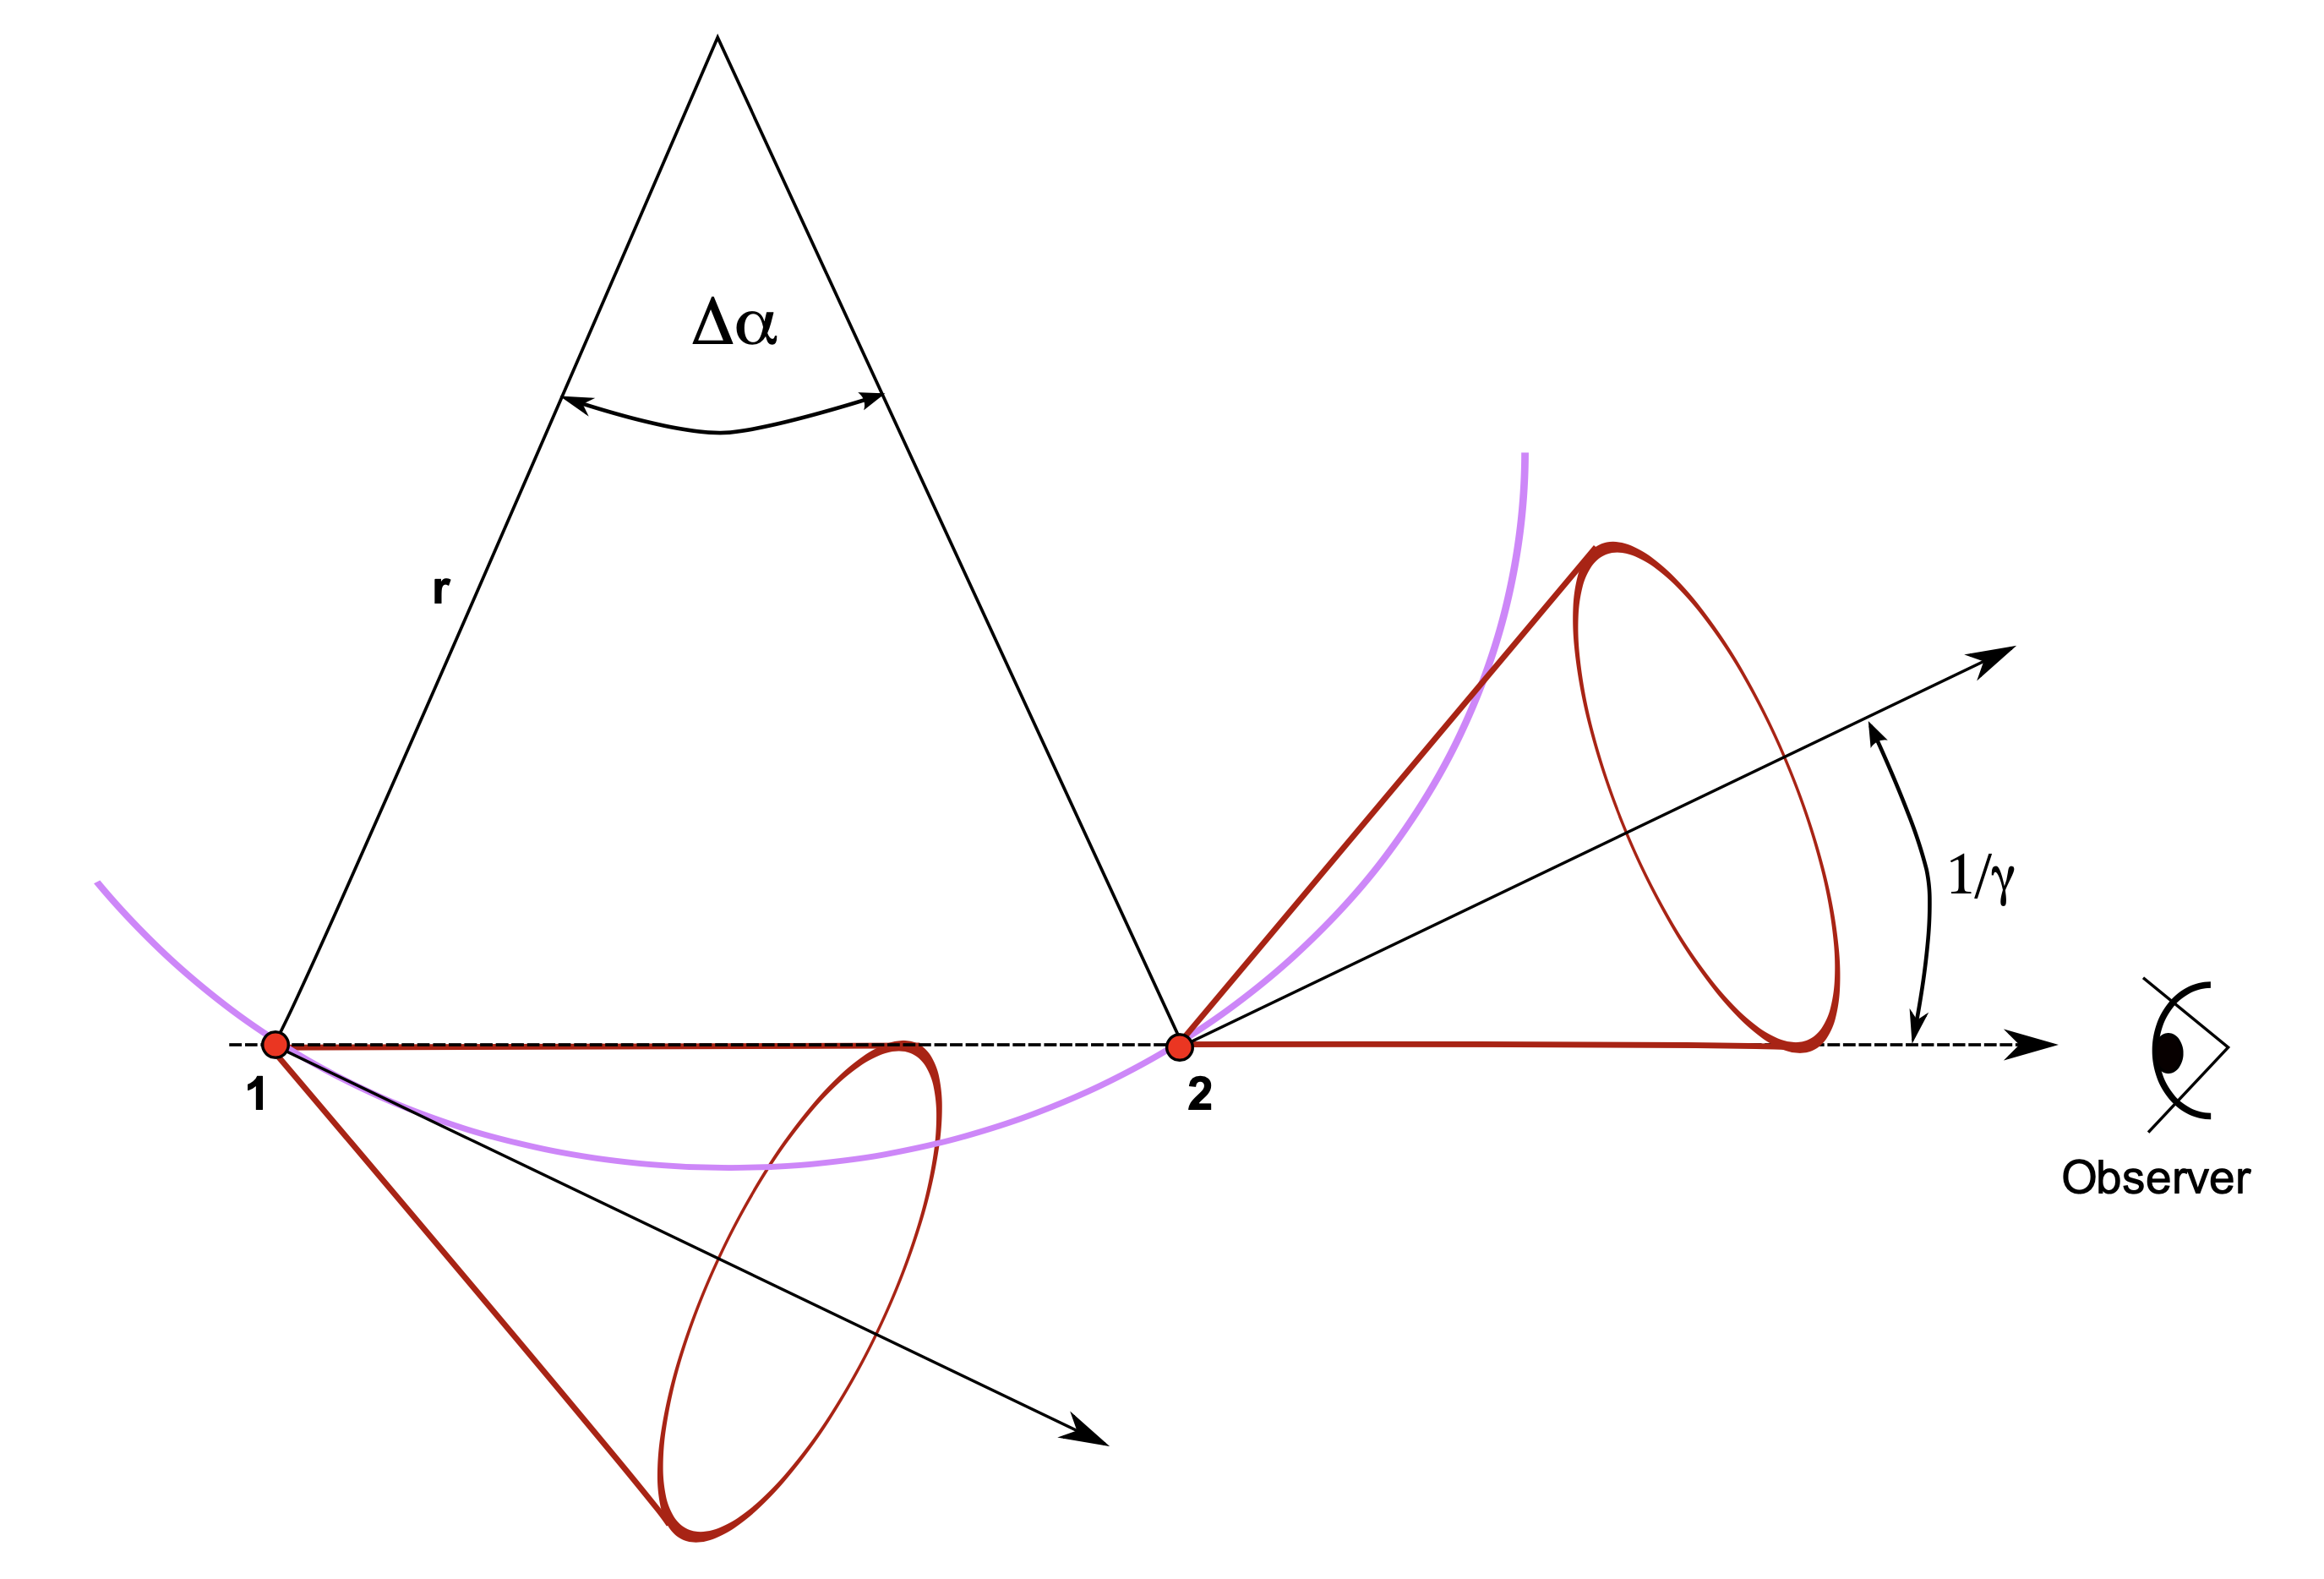
\includegraphics[width=0.8\textwidth]{opening.png}
\caption{opening}
\end{figure}

To determine the duration of emission as perceived by a distant observer, consider the time taken for an electron to move from point A to B. This segment of the trajectory corresponds to the period during which the radiation emitted by the electron falls within the observer's view because of the emitted cone:
%
\[
\Delta t = \frac{\text{AB}}{v}
\]

At the observer ($\delta t_i$ is the time for the \emph{photon} to reach the observer): 
%
\[
\Delta t_{\rm obs} = t_B + \delta t_B - (t_A  + \delta t_A) = (t_B - t_A) + (\delta t_B - \delta t_A) = \frac{\text{AB}}{v} - \frac{\text{AB}}{c} = \frac{\text{AB}}{v} (1-\beta)
\]

Using AB~$= \frac{2}{\gamma}r_{\rm L}$, we get:
%
\[
\Delta t_{\rm obs} = \frac{\text{AB}}{v} (1-\beta) \frac{1+\beta}{1+\beta} \overset{\beta \sim 1}{\simeq} \frac{\text{AB}}{v} \frac{1}{2\gamma^2} \simeq {\color{red}\frac{r_{\rm L}}{\gamma^3}}
\]

An observer sees a sequence of pulses of width:
%
\[
\Delta t_{\rm obs} \simeq \frac{1}{v \gamma^2 \nu_g} %\simeq \frac{1}{\gamma^3 \nu_L} 
\]

These pulses are separated by a gyration time 
%
\[
T \simeq \frac{1}{\nu_L} = \frac{\gamma}{\nu_g}
\]

\begin{figure}[t]
\centering
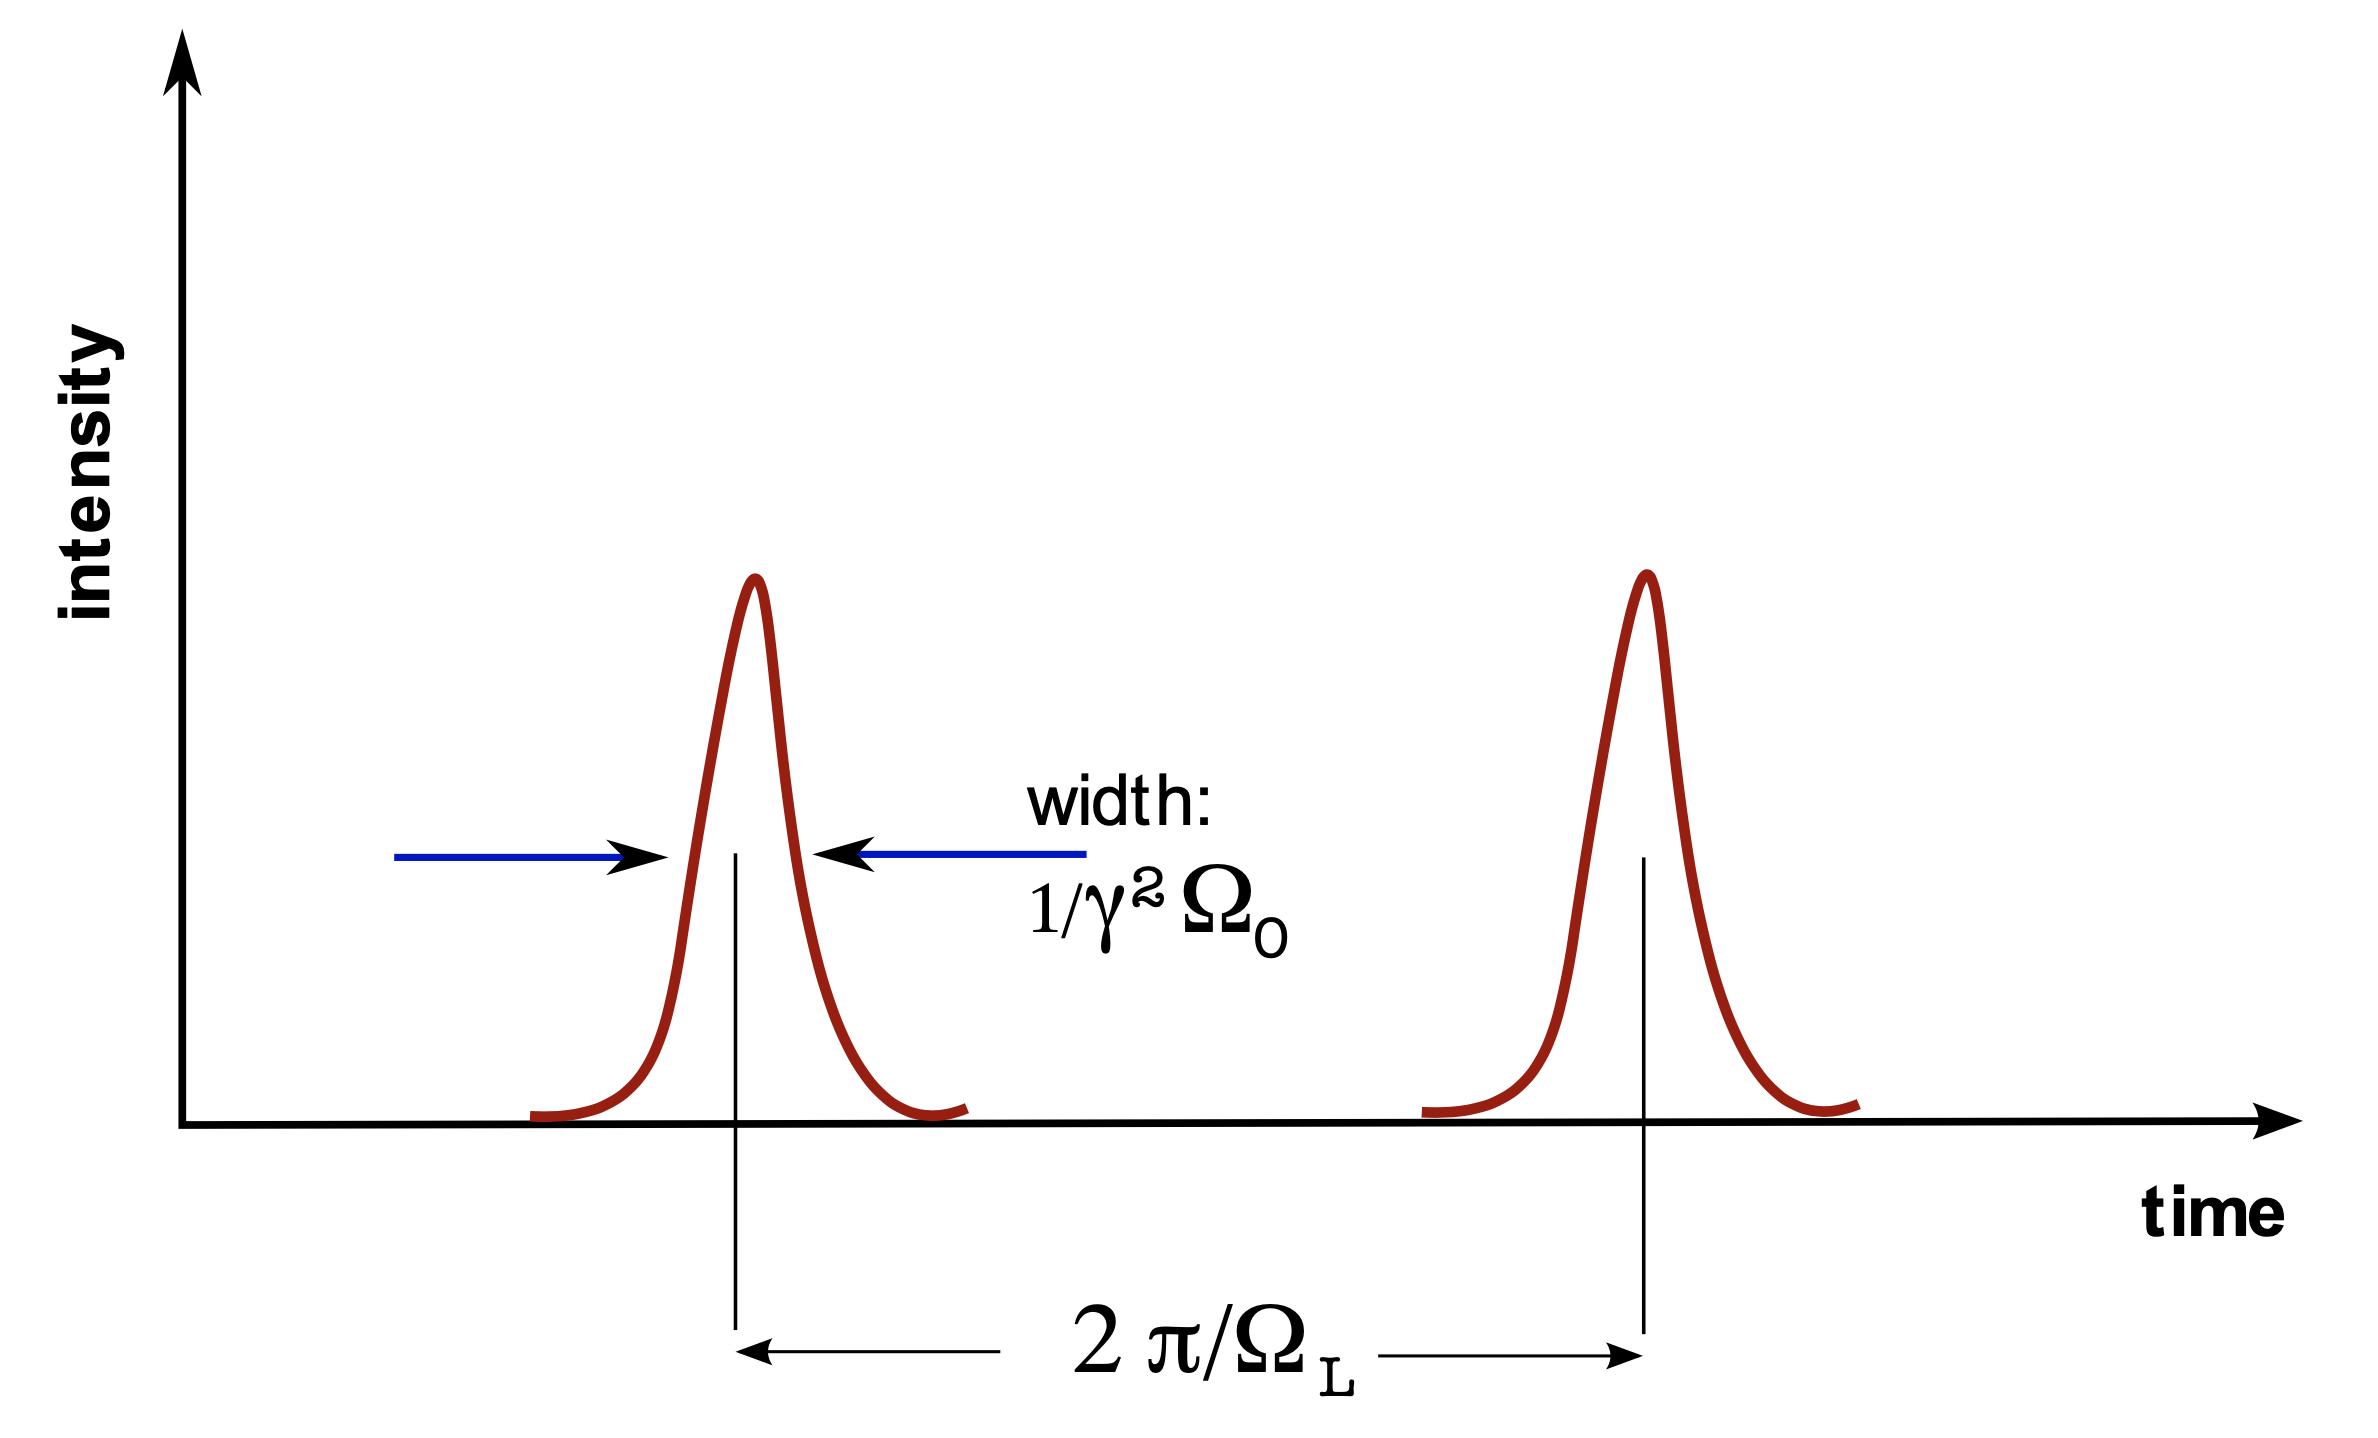
\includegraphics[width=0.8\textwidth]{observedelectricfield.png}
\caption{observedelectricfield}
\end{figure}

Thus, in the relativistic limit, the spectrum experiences a \( \gamma^2 \) boost compared to the cyclotron frequency:
%
\begin{remark}
\[
\nu_s \sim \frac{1}{\Delta t_{\rm obs}} = \frac{\gamma^3}{r_{\rm L}} = \gamma^2 \nu_g
\]
\end{remark}

\begin{problem}
Compute the properties of the Galactic radio emission.
\end{problem}

The full result for a single electron with Lorentz factor \( \gamma \) is:
%
\[
P_\nu(\nu, \gamma, \theta) = \frac{\sqrt 3 q^3 B}{m_e c^2} \sin \theta F\left(\frac{\nu}{\nu_c}\right)
\]
%
where $P_\nu$ is the power per \emph{unit of frequency}, the characteristic frequency $\nu_c = \frac{3}{4\pi} \gamma^2 \frac{qB}{m_e c} \sin \theta$, and the synchrotron function is
%
\[
F(x) = x \int_x^\infty K_{5/3} (x^\prime) dx^\prime
\]

A useful approximation for \( P_\nu \) is 
%
\[
P_\nu \simeq 1.8 \left(\frac{\nu}{\nu_c}\right)^{1/3} \exp\left(-\frac{\nu}{\nu_c}\right)
\]
%
notice that the \emph{peak} frequency is approximately  \( \nu_{\rm max} \simeq 0.29 \nu_c \).

\subsection{Quantum correction}

In our previous analysis of synchrotron radiation, we assumed that the motion of electrons does not change significantly due to photon emission. However, considering that photons carry momentum, there should be some recoil effect on the emitting electron. This aspect becomes particularly relevant when the energy of the emitted synchrotron photon, \( h \nu_s \), approaches the electron's relativistic energy, \( \gamma m_e c^2 \). Given that \( \nu_s \propto \gamma^2 \), this effect is more pronounced at higher energies.

To quantify this, we introduce the parameter \( \chi \):
%
\[
\chi = \frac{B}{B_q}\frac{p}{mc} \sim \frac{h\nu_s}{\gamma mc^2}
\]

Here, \( p \) is the electron momentum, and \( B_q = \frac{m^2 c^3}{e \hbar} \approx 4.4 \times 10^{13} \) G is a characteristic magnetic field strength.

For \( \chi \ll 1 \), the motion can be considered Newtonian, while for \( \chi \gg 1 \), quantum effects dominate. In extremely strong magnetic fields, like those found in pulsar atmospheres (\( \sim 10^{15} \) G), quantum effects become significant even for relatively low electron momenta.

According to Landau, the power radiated in the quantum regime (\( \chi \gg 1 \)) is:
%
\[
P_q \propto \frac{e^2 m^2 c^3}{\hbar^2} \left( \frac{B}{B_q}\right)^{2/3} \gamma^{2/3}
\]

This indicates that the power dependency shifts from \( \gamma^2 \) to \( \gamma^{2/3} \) in the quantum regime.

The spectrum in this regime peaks broadly and almost flatly around a frequency that satisfies:
%
\[
\frac{h\nu}{E - h\nu} \sim \chi
\]

For \( \chi \ll 1 \), the emitted frequency \( \nu \) is approximately equal to the synchrotron frequency \( \nu_s \). In contrast, for \( \chi \gg 1 \), \( h\nu \) is comparable to the initial energy \( E \), indicating that the emitted photon carries away a significant portion of the electron's energy. This results in catastrophic energy losses and a non-continuous process, necessitating a \emph{Monte Carlo} approach for accurate modeling.

\subsection{Synchrotron emission by an electron population}

Assume to have a population of electrons with a power-law distribution in energy within some given range:
%
\[
n(\gamma) d\gamma = n_0 \gamma^{-p} d\gamma \quad \gamma_{\rm min} < \gamma < \gamma_{\rm max} 
\]	
%
where $n(\gamma) d\gamma$ is the electron volume density, and usually the slope is $p \sim 2-3$.

The specific emissivity is given by
%
\begin{equation*}
j_\nu = \int_1^\infty \langle P_\nu(\gamma) \rangle n(\gamma) d\gamma
\end{equation*}
%
where $P_\nu$ is the power emitted per unit frequency.

We simplify our calculations assuming a $\delta$-function for $P_\nu$:
%
\begin{equation*}
P_\nu(\gamma) \simeq \langle P_s \rangle \delta(\nu - \nu_c)
\end{equation*}
%
follows
%
\begin{equation*}
j_\nu = \frac{4}{3} c \sigma_{\rm T} U_{\rm B} n_0 \int_{\gamma_{\rm min}}^{\gamma_{\rm max}} \gamma^{2-p} \delta(\nu - \gamma^2 \nu_{\rm L}) d\gamma
\end{equation*}
%
finally
%
\begin{remark}
\[ 
j_\nu = \frac{2}{3} c \sigma_{\rm T} n_0 \frac{U_{\rm B}}{\nu_{\rm L}} \left( \frac{\nu}{\nu_{\rm L}} \right)^{\color{red}-\frac{p-1}{2}}
\]
\end{remark}
%
which is valid in the range $\gamma^2_{\rm min} \nu_{\rm L} < \nu < \gamma^2_{\rm max} \nu_{\rm L}$

%\begin{center}
%\includegraphics[scale=0.18]{figures/synchropowerlaw.png}
%\end{center}

Outside the validity limits we have to use the complete expression and we obtain 
%
\begin{equation*}
j_\nu \propto \nu^{1/3} \quad\text{ for }\quad \nu < \nu_{\rm min}
\end{equation*}
%
and
%
\begin{equation*}
j_\nu \propto \exp \left(-\frac{\nu}{\nu_{\rm max}}\right) \quad\text{ for }\quad \nu > \nu_{\rm max}
\end{equation*}

\subsection{Kinetic equation for electron evolution}

TO BE DONE

\subsection{Synchrotron Self-Absorption}

The Synchrotron self-absorption corresponds to the inverse process where a free electron can absorb a synchrotron photon in a magnetic field $e+B+\gamma\rightarrow e+B$.

We provide here an heuristic derivation of how this process impacts on the spectrum. In fact, we have a population of electrons which are emitting radiation and absorbing radiation and we want to compute the intensity using the radiative transfer equation.

Let's remind that for a thermal distribution of electrons, the source function would correspond to the black-body
%
\[
S_\nu = {\color{red}\left(\frac{2\nu^2}{c^2}\right)} {\color{blue}\left(\frac{h\nu}{\exp(h\nu / kT) - 1}\right)} 
\propto {\color{red}\nu^2} {\color{blue}\langle E \rangle}
\]
%
where the first term is the \emph{phase-space factor} and the second is the \emph{mean electron energy} emitting photons at frequency $\nu$.

In fact, in the Rayleigh-Jeans limit $kT \gg h\nu$ and
%
\[
\langle E \rangle \simeq kT \lim_{x\rightarrow 0} \frac{x}{\exp x - 1} \sim kT
\]

For a non-thermal synchrotron radiation $kT$ must be replaced by the mean energy of an electron emitting synchrotron radiation at frequency $\nu$
%
\begin{equation*}
\nu \simeq \gamma^2 \nu_{\rm L} \rightarrow \gamma \sim \left(\frac{\nu}{\nu_{\rm L}}\right)^{1/2}
\end{equation*}
%
follows
%
\begin{equation*}
S_\nu \sim \left( \frac{2\nu^2}{c^2} \right) \gamma m_e c^2
\propto \left( \frac{2\nu^2}{c^2} \right) \left(\frac{\nu}{\nu_{\rm L}}\right)^{1/2} 
\propto B^{-1/2} \nu^{5/2} 
\end{equation*}

%\begin{center}
%\includegraphics[scale=0.06]{figures/x299.png}
%\end{center}

From the definition of the source term \( S_\nu = \frac{j_\nu}{\alpha_\nu} \), follows
%
\[
\alpha_\nu = \frac{j_\nu}{S_\nu} 
\propto (B^{\frac{p+1}{2}} \nu^{-\frac{p-1}{2}}) (B^{\frac 1 2} \nu^{-\frac 5 2})
= B^{\frac{p+2}{2}} \nu^{-\frac{p + 4}{2}}
\]

We notice that $\alpha_\nu$ decreases towards higher frequencies, so it will be relevant at low energies.

From the transfer equation $I_\nu = S_\nu [1 - \exp(-\tau_\nu)]$ and reminding $\tau_\nu = \alpha_\nu s$, we identify the following limiting regimes:
%
\begin{itemize}
\item for $\tau_\nu \gg 1$ corresponding to small frequencies $I_\nu \rightarrow S_\nu$

\item for $\tau_\nu \ll 1$ corresponding to large frequencies $I_\nu \rightarrow S_\nu \alpha_\nu s = j_\nu s$
\end{itemize}

Therefore for each source exists a frequency $\nu_B$ where $\tau_B = 1$ and the corresponding spectrum will be:
%
\begin{itemize}
\item for $\nu \ll \nu_B$ (optically thick) and $I_\nu \propto \nu^{5/2}$, notice independent on $p$!

\item for $\nu \gg \nu_B$ (optically thin) and $I_\nu \propto \nu^{-\frac{p-1}{2}}$
\end{itemize}

% TYPICAL SPECTRUM OF A RADIO SOURCE

\begin{problem} Estimate the age of the source from the break.
\end{problem}

%As our observing frequency increases, we see photons coming from regions of the source that are progressively deeper and deeper, and as we do so the total flux density increases. However, of course, eventually we reach a point where we can “see all the way through” the plasma, and above this frequency we recover the underlying power-law distribution.

%\begin{center}
%\includegraphics[scale=0.14]{figures/selfabsorption.png}
%\end{center}

%Representative spectra of \textbf{radio galaxies and quasars}. The radio source 3C 84 in the nearby galaxy NGC 1275 contains a very compact nuclear component that is opaque below about 20 GHz. The radio galaxy 3C 123 is transparent at all plotted frequencies, and energy losses steepen its spectrum above a few GHz. The quasar 3C 48 is synchrotron self-absorbed only below 100 MHz, while the quasar 3C 454.3 contains structures of different sizes that become opaque at different frequencies.

\subsection{Minimum Energy and Equipartition}

The existence of a synchrotron source implies the presence of relativistic electrons with some energy density $U_{\rm e}$ and a magnetic field whose energy density is $U_{\rm B} = \frac{B^2}{8\pi}$. 
%
What is the \emph{minimum total energy in relativistic particles and magnetic fields} required to produce a synchrotron source of a given radio luminosity?

The energy density in particles is
%
\[
U_e = \int_{\gamma_{\rm min}}^{\gamma_{\rm max}} E n(\gamma) d\gamma
%\simeq n_0 m_e c^2 \int_{\gamma_{\rm min}}^{\infty} \gamma^{1-p} d\gamma n_0 m_e c^2 = \frac{n_0 m_e c^2}{p-2} \gamma_{\rm min}^{-(p-2)}
\]
%
and the corresponding luminosity is
%
\[
\mathcal L = V \int_{\gamma_{\rm min}}^{\gamma_{\rm max}} \left| \frac{dE}{dt} \right| n(\gamma) d\gamma
%\simeq n_0 m_e c^2 \int_{\gamma_{\rm min}}^{\infty} \gamma^{1-p} d\gamma n_0 m_e c^2 = \frac{n_0 m_e c^2}{p-2} \gamma_{\rm min}^{-(p-2)}
\]

For a power-law distribution $n(\gamma) \propto \gamma^{-p}$, and using $P \propto \gamma^2 U_B$ the ratio between the two is proportional to
%
\begin{equation*}
\frac{U_e}{\mathcal L} \propto \frac{1}{U_B} \frac{\int_{\gamma_{\rm min}}^{\gamma_{\rm max}} \left( \frac{\gamma}{\gamma_{\rm min}}\right)^{1-p} d\gamma}{\int_{\gamma_{\rm min}}^{\gamma_{\rm max}}  \left( \frac{\gamma}{\gamma_{\rm min}}\right)^{2-p}  d\gamma} \propto \frac{1}{U_B} \frac{\gamma_{\rm min}^{2-p}}{\gamma_{\rm min}^{3-p}} \propto \frac{1}{U_B \gamma_{\rm min}}
\end{equation*}	

Finally, $\nu_s \propto \gamma^2 B$ therefore $\gamma \propto B^{-1/2}$, for a fixed frequency, and thereby $U_e / \mathcal L \propto B^{-3/2}$.  

We conclude that the electron energy density needed to produce a given synchrotron luminosity scales as $U_e \propto B^{-3/2}$. % while the magnetic energy density $U_B \propto B^2$.

The minimum of the total energy density $U$ as a function of $B$ occurs at
%
\begin{equation*}
\frac{dU}{dB} = \frac{d}{dB} (U_e + U_B) = 0 \rightarrow \frac{-3/2}{B} U_e + \frac{2}{B} U_B = 0
\end{equation*}

The ratio of cosmic-ray particle energy density to magnetic field energy that minimizes the total energy is
%
\begin{remark}
\[
\frac{U_e}{U_B} = \frac{4}{3}
\]
\end{remark}

This ratio is nearly unity, so minimum energy constraint for an optically thin synchrotron source places similar amount of energy in particles as in magnetic fields (equipartition).

\begin{problem}
Cygnus A (3C 405)
\end{problem}

%Physical motivated.
% !TEX root = ../lectures.tex
\section{Inverse Compton Scattering}

The IC process involves the up-scattering of background photons by high-energy (HE) electrons (\(e + \gamma \rightarrow e' + \gamma'\)). It is a significant energy loss mechanism for electrons if their energy exceeds that of the photons.

To derive the power emitted during IC scattering, we initially approach from a classical perspective before discussing quantum interpretations.

In the classical view, an electromagnetic wave strikes an electron, causing it to oscillate and thus radiate power due to acceleration. The Poynting flux (\( \vb S \)) of a plane wave incident on an electron is:
%
\[
\vb S =  \frac{c}{4\pi} \vb E \times \vb B \rightarrow S = \frac{c}{4\pi} | \vb E |^2   
\]

The Lorentz force acting on the electron is:
%
\[
\vb F = q (\vb E + \frac{\vb v}{c} \times \vb B) \simeq q \vb E
\]
%
assuming \( | \vb v | \ll c \).

The oscillating electric field of the wave is:
%
\[
\vb E = E_0 \vb \epsilon \sin (\omega t + \phi)
\]
%
leading to an average acceleration:
%
\[
\vb a = \frac{\vb F}{m} \rightarrow \langle a^2 \rangle = \frac{q^2}{m^2} \frac{E_0^2}{2}
\]
%
where we used
%
\[
\frac{1}{T} \int_0^{T = \frac{2\pi}{\omega}} \sin^2 (\omega t) dt = \frac{1}{2}
\]

Thus, the average power radiated by the electron is:
%
\[
\langle P \rangle = \frac{2}{3} \frac{q^2 a^2}{c^3} = \frac{2}{3} \frac{q^2}{c^3} \frac{a^2}{m^2} \frac{E_0}{2} = \frac{1}{3} \frac{q^4}{m^2 c^3} E_0^2
\]

The classical cross-section associated to this process is the \emph{ratio} between the power radiated and the impinging flux
%
\begin{remark}
\begin{equation*}
\langle P \rangle = \sigma_{\rm T} \langle | \vb S | \rangle \rightarrow \sigma_{\rm T} = \frac{1}{3} \frac{q^4}{m^2 c^3} E_0^2 \frac{8\pi}{c} \frac{1}{E_0^2} = \frac{8}{3} \pi \left( \frac{q^2}{m c^2} \right)^2
\end{equation*}
\end{remark}
%
where we use the average Poynting flux $\langle \vb S \rangle = \frac{c}{8\pi} E_0^2$.

This is known as Thomson cross-section and its numerical value is 
%
\begin{equation*}
\sigma_{\rm T} \simeq 6.652 \cdot 10^{-25}~\text{cm}^2
\end{equation*}

In other words, the electron will extract from the incident radiation the amount of power flowing through the area $\sigma_T$ and reradiate that power over the doughnut-shaped pattern given by Larmor’s equation.

%The classical cross-section associated with this process, known as the Thomson cross-section, is:
%\[
%\sigma = \frac{8}{3} \pi \left( \frac{q^2}{m c^2} \right)^2
%\]

%This implies the electron extracts and reradiates power from the incident radiation flowing through an area equal to the Thomson cross-section (\( \sigma_{\rm T} \)).

The time-averaged scattered power by a single particle is:
%
\[
P = \sigma_{\rm T} c U_{\rm rad}
\]
%
where \( U_{\rm rad} = S /c \) is the energy density of the incident radiation.

Incidentally, the Thomson optical depth, representing the probability of a photon undergoing Thomson scattering (notice this is the opposite process!) is:
%
\[
\tau_e = \int n_e \sigma_{\rm T} ds
\]

\begin{problem}
The Intergalactic Medium (IGM) at redshifts \( z \lesssim 10 \) is observed to be highly ionized, likely due to radiation from galaxies and quasars. Post-recombination at \( z \approx 10^3 \), the IGM was almost completely neutral. This observation indicates that reionization of the IGM occurred somewhere \( z_r \gtrsim 10 \), although the exact timing of this crucial transition remains unknown. 

An ionized IGM Thomson scatters CMB photons. Under the assumption of a uniform Universe with a specified baryon fraction \( \Omega_b \) in units of the critical density \( \Omega_c \), derive the relation between \( \tau_r \) and \( z_r \) and calculate \( \tau_r \) assuming a reionization redshift \( z_r = 10 \) for an Einstein-de Sitter Universe.
\end{problem}

The Compton scattering process, involving the interaction of photons with electrons, can be effectively described using quantum mechanics.

We start by imposing the energy and momentum balance in the scattering process:
%
\[
K_i^\mu + P_i^\mu = K_f^\mu + P_f^\mu
\]
%
where \( P_{i,f}^2 = m_e^2 \) and \( K_{i,f}^2 = 0 \) (for photons).

Contracting the final momentum gives:
%
\[
 P_f^\mu P_{f \mu} = (P_i + K_i - K_f)^\mu (P_i + K_i - K_f)_\mu  \rightarrow m_e^2 = m_e^2 + 2 (P_i K_i - P_i K_f - K_i K_f)
\]

In the frame where the electron is initially at rest \( P_i = \left( m_e, \vb 0 \right) \), and assuming the x-axis is aligned with the incoming photon, we have:
%
\[
K_i = \epsilon_i (1, 1, 0, 0) \quad \text{and} \quad K_f = \epsilon_f (1, \cos \theta, \sin \theta, 0)
\]

Substituting these into the equation, we get:
%
\[
m_e^2 = m_e^2 + 2 \left( m_e \epsilon_i - m_e \epsilon_f - \epsilon_i \epsilon_f + \epsilon_i \epsilon_f \cos \theta \right)
 \rightarrow m_e (\epsilon_i - \epsilon_f) = \epsilon_i \epsilon_f (1-\cos\theta)    
\]

Leading to the relation for the final photon energy:
%
\begin{remark}
\[
\epsilon_f = \frac{\epsilon_i}{1+ \frac{\epsilon_i}{m_e c^2} (1-\cos\theta)}
\]
\end{remark}

The fractional energy change of the photon is:
%
\[
\frac{\Delta \epsilon}{\epsilon}  
= \frac{\epsilon_f - \epsilon_i}{\epsilon_i} = -1 + \frac{1}{1 + \frac{\epsilon_i}{m_e c^2} (1-\cos\theta)} \overset{\epsilon_i \ll m_e c^2}{\longrightarrow} - \frac{\epsilon_i}{m_e c^2} (1-\cos\theta)
\]

This equation describes \emph{Compton scattering}, where a photon scatters off an electron and transfers energy, resulting in a decrease in photon energy. Notably, unless the photon's energy is comparable to or larger than the electron mass in the electron's rest frame, the photon energy is only slightly altered.

Thomson scattering accurately describes the regime where the incident photon energy \( \epsilon_i \) is much less than the electron rest energy (\( \epsilon_i \ll m_e c^2 \)). In this regime, energy transfer is minimal, \( \epsilon_i \simeq \epsilon_f \), indicative of quasi-elastic scattering.

However, as \( \epsilon_i \) approaches or exceeds \( m_e c^2 \), the energy transfer becomes significant, marking a transition to deeply inelastic scattering. This regime is governed by the Klein-Nishina (KN) cross-section.

The full Klein-Nishina cross-section, derived using Quantum Electrodynamics (QED), is given by:
%
\[
\sigma_{\rm KN} = \frac{3}{4} \sigma_{\rm T} \left[ \frac{1+x}{x^3} \left(\frac{2x(1+x)}{1+2x} - \ln (1+2x)\right) + \frac{1}{2x} \ln (1+2x) - \frac{1+3x}{(1+2x)^2} \right]
\]
%
where \( x = \epsilon_i / m_e c^2 \).

In the limit of \( x \ll 1 \), the equation converges to the Thomson limit \[ \sigma(x) \simeq \sigma_{\rm T} (1-2x+\dots) \] while in the extreme KN limit (\( x \gg 1 \)), it approaches \[ \sigma(x) \simeq \frac{3}{8} \sigma_{\rm T} \frac{1}{x} (\ln 2x + \frac{1}{2}) \]

Therefore, the principal effect of the KN regime is a reduction in the cross-section relative to the classical Thomson value as the photon energy increases.

%%% PLOT

When the electron involved in Compton scattering has a velocity \( \beta \) in the laboratory (LAB) frame, the scattering dynamics change.

The relationship in the electron's rest frame (primed frame) remains valid:
%
\[
\epsilon^\prime_f = \frac{\epsilon^\prime_i}{1+ \frac{\epsilon^\prime_i}{m_e c^2} (1-\cos\theta^\prime)}
\]
%
where \( \theta^\prime \) is the angle between incoming and outgoing photon directions in the primed frame. Applying Lorentz transformation:
%
\[
\epsilon'_i = \epsilon_i \gamma (1-\beta \cos \alpha)
\]
%
where \( \alpha \) is the angle between the photon and electron in the LAB frame.

To express \( \epsilon^\prime_f \) in the LAB frame and account for the emission angle \( \alpha^\prime \) in the comoving frame:
%
\[
\epsilon_f = \gamma(1+\beta \cos\alpha^\prime) \epsilon^\prime_f = 
\gamma (1+\beta \cos \alpha^\prime) \frac{\epsilon^\prime_i}{1+ \frac{\epsilon^\prime_i}{m_e c^2} (1-\cos\theta^\prime)}
\]
%
or
\[
\epsilon_f = \gamma^2 \epsilon_i \frac{(1+\beta \cos\alpha^\prime)(1-\beta \cos\alpha)}{1+ \frac{\epsilon^\prime_i}{m_e c^2} (1-\cos\theta^\prime)}
\]

In the limit \( \epsilon_i \ll m_e \) (or equivalently \( \gamma \epsilon_i \ll m_e c^2 \) or \( E_e \epsilon_i \ll m_e^2 c^4 \) in the LAB frame):
%
\[
\epsilon_f \simeq \gamma^2 \epsilon_i (1+\beta \cos\alpha^\prime)(1-\beta \cos\alpha)
\]

For isotropic incident and outgoing radiation in the electron's comoving frame, the average final energy is approximately 
%
\begin{remark}
\[
 \epsilon_f \simeq \gamma^2 \epsilon_i \simeq 4 \left(\frac{\epsilon_i}{\rm eV}\right)\left(\frac{E_e}{\rm GeV}\right)^2 \, \text{MeV}   
\]
\end{remark}

While the scattering angle is arbitrary in the \emph{comoving} frame, in the LAB frame, the outgoing radiation is \emph{beamed} in the forward direction with an angle \( \frac{1}{\gamma} \).

In the Thomson regime (\( \epsilon^\prime_i \ll m_e \)), the maximum final photon energy, when \( \beta \sim 1 \), \( \cos \alpha^\prime \sim 1 \), and \( \cos \alpha \sim - 1 \), is:
%
\[
\epsilon_{f} \sim 4 \gamma^2 \epsilon_i
\]

In the KN limit, the typical energy of the outgoing photon is:
%
\[
\epsilon_f \simeq \frac{\gamma^2 \epsilon_i}{1 + \frac{\epsilon^\prime_i}{m_e}} \simeq \frac{\gamma^2 \epsilon_i}{\epsilon^\prime_i} m_e \simeq \frac{\gamma^2 \epsilon_i}{\gamma \epsilon_i} m_e \simeq E_e
\]

This implies that in the extreme KN regime, the scattering becomes less frequent, but when it occurs, the scattered photon carries away a significant fraction of the electron's energy.

\begin{remark}
In summary, in the LAB frame:
%
\begin{itemize}
\item In the Thomson regime: \( \epsilon_f \simeq \gamma^2 \epsilon_i \) for \( \gamma \epsilon_i \ll m_e c^2 \)
\item In the KN regime: \( \epsilon_f \simeq \gamma m_e c^2 \) for \( \gamma \epsilon_i \gg m_e c^2 \)
\end{itemize}
\end{remark}

\subsection{Single particle power radiated in IC scattering}

In the Thomson regime, namely $\epsilon'_i \ll m_e c^2$, the power re-emitted by scattering is $\frac{dE}{dt} \simeq \sigma_{\rm T} c U_{\rm rad}$.

We consider now radiation scattering by an ultrarelativistic electron. This expression is still valid in the primed frame instantaneously moving with the electron
%
\begin{equation*}
\frac{dE'}{dt'} = \sigma_{\rm T} c U'_{\rm rad}
\end{equation*}
%
and we want to transform in the LAB frame.

 We recall that the power is LI as it is the ratio of two time-like components, thereby
\begin{equation*}
 \frac{dE}{dt} = \frac{dE'}{dt'} = \sigma_{\rm T} c U'_{\rm rad}
\end{equation*}

The photon density can be seen as the number density of photon of energy $\epsilon$, that is
%
\begin{equation*}
U'_{\rm rad} \simeq 
\int n'_\gamma(\epsilon'_i) \epsilon'_f(\epsilon'_i, \theta) d\epsilon'_i
\end{equation*}
%
where $n'_\gamma(\epsilon') d\epsilon'$ is the number density of incident photons with energy $\epsilon' \rightarrow \epsilon' + d\epsilon'$ \, .

%which is the total power emitted by an electron exposed to some photonfield $n_\gamma(\epsilon)$, 

Similarly, the phase-space distribution is LI as $f (\vb x, \vb p) = \frac{dN}{d^3\vb x d^3 \vb p} = f'(\vb x', \vb p')$, therefore $n(\epsilon) d\epsilon = f d^3 \vb p$ transforms as $d^3 \vb p$ which transforms as an energy, follows
%
\begin{equation*}
\frac{n_\gamma(\epsilon) d\epsilon}{\epsilon} = \frac{n_\gamma(\epsilon') d\epsilon'}{\epsilon'}
\end{equation*}

finally, reminding that in Thomson $\epsilon'_i \simeq \epsilon'_f$ (we are in the electron frame!)

\begin{equation*}
U'_{\rm rad} 
\simeq \int n^\prime_\gamma(\epsilon^\prime_i) {\color{red}\epsilon^\prime_i}  d\epsilon^\prime_i 
= \int \epsilon_i^{\prime 2} \frac{n_\gamma(\epsilon_i)}{\epsilon_i} d\epsilon_i 
% %= \int \epsilon'_i^2 \frac{n'_\gamma(\epsilon'_i)}{\epsilon'_i} d\epsilon'_i 
= \int \epsilon_i^2 \gamma^2 (1-\beta\cos\theta)^2 \frac{n_\gamma(\epsilon_i)}{\epsilon_i} d\epsilon_i 
\end{equation*}

Assuming isotropic incident radiation field
%
\begin{equation*}
\frac{1}{2} \int_{-1}^{1} (1-\beta \cos \theta)^2 d\cos\theta = \frac{1}{2} \int_{-1}^{1} (1-2\beta\cos\theta + \beta^2\cos^2\theta) d\cos\theta = 1 + \frac{\beta^2}{3}
\end{equation*}
%
\begin{equation*}
U'_{\rm rad} = \gamma^2 \left(1 + \frac{\beta^2}{3}\right) U_{\rm rad}
\end{equation*}

therefore the angle-averaged Compton scattered power (in the LAB frame) is
%
\begin{equation*}
\frac{dE}{dt} = \sigma_{\rm T} c U'_{\rm rad} = \sigma_{\rm T} c \gamma^2 \left( 1 + \frac{\beta^2}{3} \right) U_{\rm rad} 
\end{equation*}

We are not done yet! The energy \emph{lost by the electron} and \emph{gained by the photons} is the up-scattered power (power in the final photon field) minus the scattered power (power in the initial photon field)
%
\begin{equation*}
\frac{dE_e}{dt} 
= \sigma_{\rm T} c U'_{\rm rad} - \sigma_{\rm T} c U_{\rm rad}
\end{equation*}

This leads to the IC power as
%
\begin{equation*}
P_{\rm IC} = \sigma_{\rm T} c \left(\gamma^2 +\frac{\gamma^2 \beta^2}{3} -1 \right) U_{\rm rad} = \frac{4}{3}
\sigma_{\rm T} c \beta^2 \gamma^2 U_{\rm rad}
\end{equation*}
%
where I used $\gamma^2 - 1 = \beta^2 \gamma^2$

This is the \emph{net inverse-Compton power gained by the radiation field and lost by the electron}. 

The similarity of the inverse Compton and synchrotron equations shouldn’t be too surprising: they both describe the interaction of an electron with an electromagnetic field.

Note that synchrotron and inverse-Compton losses have the same electron-energy dependence, so their effects on  spectra are indistinguishable.

Dividing by the corresponding synchrotron power 
%
\begin{remark}
\[
\frac{P_{\rm IC}}{P_{\rm s}} = \frac{U_{\rm rad}}{U_{\rm B}}    
\]
\end{remark}
%
which is valid if no absorption and no KN effects are relevant.

What is the average energy increase in the Thomson regime? 

 The number of photons scattered per unit time are
%
\begin{equation*}
\frac{dN_s}{dt} \simeq \frac{\sigma_{\rm T} c U_{\rm rad}}{\langle \epsilon_i \rangle}
\end{equation*}

The average energy increase can be written as
%
\begin{equation*}
P_{\rm IC} \simeq \langle \epsilon_f \rangle \frac{dN_s}{dt} \rightarrow \epsilon_f = \frac{P_{\rm IC}}{dN_s/dt} = \frac{4}{3} \gamma^2 \beta^2 \epsilon_i \simeq {\color{red}\frac{4}{3} \gamma^2 \epsilon_i}
\end{equation*}

If the energy transfer in the K' frame is not neglected (KN regime)
%
\begin{equation*}
- \frac{dE_e}{dt} = P_{\rm IC} = \frac{4}{3} \gamma^2 \beta^2 \sigma_{\rm T} c U_{\rm rad} \left[1 - \frac{63}{10} \frac{\gamma}{m_e c^2} \frac{\langle \epsilon_i^2 \rangle}{\langle \epsilon_i \rangle} + \dots \right]
\end{equation*}
%
where $<\epsilon_i> = \frac{\int \epsilon_i n_\gamma(\epsilon_i) d\epsilon_i}{\int n_\gamma(\epsilon_i) d\epsilon_i}$, which is obtained for incident isotropic photon distribution (see Blumenthal and Gould, 1970).

 Notice that in this regime the photon-field  distribution is relevant (not only the total density as before).
% !TEX root = ../lectures.tex
\section{Gamma-ray Absorption}

\begin{figure}[t]
\centering
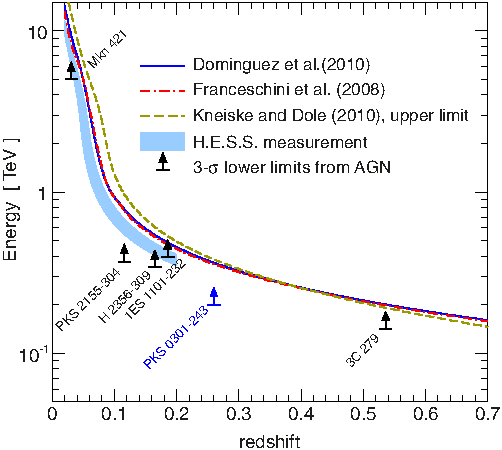
\includegraphics[width=0.5\textwidth]{figures/aa21639-13-fig6.pdf}
\caption{$\gamma$-ray horizon for differen EBL models. Some lower limits from AGN spectra measurements are shown~\cite{HESS2013aa}.}
\end{figure}

Extra-galactic gamma-rays undergo absorption during intergalactic propagation by interacting with photons in the diffuse radiation field, producing electron-positron pairs (\(\gamma + \gamma \rightarrow e^+ + e^-\)). This process depends on the energy threshold condition for opacity.

The square of the center-of-mass (COM) energy, \( s \), is a relativistic invariant:
%
\[
s = (P_a + P_b)^2 = m_a^2 + m_b^2 + 2(E_a E_b - \vb p_a \cdot \vb p_b) = m_a^2 + m_b^2 + 2E_a E_b (1 - \beta_a \beta_b \cos \theta)    
\]

For head-on collisions in the pair-production process \(\gamma + \gamma \rightarrow e^+ e^-\), the threshold energy in the LAB frame is:
%
\[
s = 2 E_\gamma \epsilon (1 + 1) = (2 m_e)^2 \rightarrow 4E_\gamma \epsilon = (2 m_e)^2 \rightarrow E_\gamma > \frac{m_e^2}{\epsilon}    
\]

For instance, a 1 TeV photon (\(E_\gamma = 10^{12}\) eV) interacts at the threshold with infrared photons (\(\epsilon \gtrsim 0.26\) eV).

The cross-section for pair-production, \(\sigma_{\gamma \gamma}(\beta^*)\), is given by:
%
\[
\sigma_{\gamma \gamma}(\beta^*) = \frac{3}{16} \sigma_{\rm T} (1-\beta^{*2}) \left[2 \beta^* (\beta^{*2}-2) + (3-\beta^{*4}) \ln \left( \frac{1+\beta^*}{1-\beta^*} \right) \right]
\]
%
where \(\beta^*\) is the velocity of the electron (or positron) in the CoM frame. 

The velocity \(\beta^*\) is determined by comparing the CoM energy with the energy in the CoM frame:
%
\[
2E_\gamma \epsilon(1- \cos\theta) = 4 E_e^{*2} \rightarrow \beta^* = \sqrt{1 - \frac{2 m_e^2 c^4}{E_\gamma \epsilon (1-\cos\theta)}}
\]
%
where I used
%
\[
E_e^* = \gamma^* m_e c^2 = \frac{1}{(1-\beta^{*2})^{1/2}} m_e c^2 = \sqrt{1 - \frac{2 m_e c^4}{x}}
\]

The cross-section reaches a maximum at \(x = 4 m_e c^4\), corresponding to \(\sigma(x) \simeq \sigma_{\rm T}/4\).

A 1 TeV photon most efficiently interacts with \(\sim 1\) eV photons. In the high-energy limit, the cross-section becomes inversely proportional to the energy product:
%
\[
\sigma_{\gamma\gamma}(\beta^*) \simeq \frac{3}{8} \frac{\sigma_{\rm T}}{\gamma^{*2}} \left[ \ln(4\gamma^{*2}) - 1\right] \propto \frac{1}{\gamma^{*2}} \simeq \frac{1}{E_\gamma \epsilon}
\]

That means that $\gamma$-rays can interact with all photons above the threshold but the cross-section decreases as $\epsilon$ increases (near threshold process).

The optical depth for \(\gamma\gamma\) absorption, \(\tau_{\gamma\gamma}(E_\gamma)\), takes into account all photons above the threshold:
%
\[
\tau_{\gamma\gamma}(E_\gamma) = \int_0^R \int_{4\pi} d\Omega (1-\cos\theta) \int_{\epsilon_{\rm th}}^\infty d\epsilon n_\gamma(\epsilon, \Omega, x) \sigma_{\gamma\gamma}(E_\gamma, \epsilon, \cos\theta)
\]

%%% PLOT WITH BACKGROUND FIELDS

%%% PLOT WITH SIGMA(X)

%%% PLOT WITH OPTICAL DEPTH

\subsection{Electromagnetic cascades}

TO BE DONE

% !TEX root = ../main.tex
\section{Nuclei-proton Interactions}

Nucleon-nucleon and nucleus-nucleus reactions are governed by the strong force, a short-range interaction. Unlike leptons and photons, nucleons and nuclei are extended objects with radii approximately $R_N \sim 1.2 A^{1/3}$~fm. This results in interaction cross-sections of the order of the geometrical cross-section $\sigma_{\rm geom} \simeq \pi R_N^2 \simeq 45 A^{2/3}$~mb\footnote{As reference value $1~\text{mb} = 10^{-27}~\text{cm}^2 \sim \frac{\sigma_{\rm T}}{500}$.}, which is a valid rule of thumb~\cite{Letaw1983apjs}.

Therefore, in regions with increased target density, such as the inner regions of starburst galaxies or galactic molecular clouds, one can estimate the timescale of high-energy nuclei interacting with gas targets as
%
\[
\tau \simeq \frac{1}{n_{\rm t} \sigma_{\rm geo} c} \simeq 25 \, A^{-2/3} \left( \frac{n_{\rm H}}{\text{cm}^{-3}} \right)^{-1}~\text{Myr}
\]
%
This timescale proves competitive when compared to other processes, such as particle escape or other forms of energy loss.

A significant portion of astrophysical gamma rays and neutrinos originate from the decay of pions, which are generated in interstellar collisions where protons serve as both targets and projectiles.

High-energy proton interactions primarily result in the following final states:
%
\[
p + p \rightarrow 
\begin{cases}
p + p + \pi^0 \\
p + n + \pi^+ \\
p + p + \pi^+ + \pi^- 
\end{cases}
\]

The production of neutral pions $\pi^0$ leads to gamma-ray radiation through the decay 
%
\[ 
\pi^0 \rightarrow {\color{red}\gamma} + {\color{red}\gamma} 
\]

The decay of charged pions, followed by the secondary muon decay, generates a total of 3 neutrinos in the final state as 
%
\begin{eqnarray*}
\pi^+ & \rightarrow & {\color{red}\nu_\mu} + \mu^+ \\
& & \hphantom{\nu_\mu + l} \drsh \, e^+ + {\color{red}\bar \nu_\mu} + {\color{red}\nu_e} \\
\pi^- & \rightarrow & {\color{red}\bar \nu_\mu} + \mu^- \\
& &  \hphantom{\bar \nu_\mu + l} \drsh \, e^- + {\color{red}\nu_\mu} + {\color{red}\bar \nu_e} 
\end{eqnarray*}

In this scenario, the same mechanism that generates high-energy photons also produces neutrinos. Consequently, the presence of neutrinos serves as a definitive indicator of hadronic processes, distinguishing them from processes primarily involving leptons, which do not produce neutrinos.

The energy threshold for $\pi^0$-production in the proton-proton collision is determined by
%
\[
2 m_p^2 + 2 E^{\rm th}_p m_p = \left(2 m_p + m_{\pi^0} \right)^2
\]
%
where $E^{\rm th}_p$ is the proton energy threshold in the LAB frame.

Using $m_p = 0.938$~GeV, and $m_{\pi^0} = 0.135$~GeV, one obtains
%
\begin{equation}
E_p^{\rm th} = m_p + 2 m_\pi + \frac{m_\pi^2}{2 m_p} \simeq 1.22~\text{GeV}
\end{equation}
%
or, in terms of kinetic energy,
%
\begin{equation}
T_p^{\rm th} = E_p^{\rm th} - m_p \simeq 280~\text{MeV}
\end{equation}

The inelastic cross-section for proton-proton collisions, denoted as \(\sigma_{\rm pp}\), has been accurately measured in terrestrial accelerators, with a clear dependence on the proton energy in the laboratory frame. This cross-section rapidly increases from the particle production threshold, reaching several tens of mb's at proton energies of a few GeV, and thereafter exhibits a more gradual increase with energy.

A convenient parametrization for the total inelastic cross-section can be found in~\cite{Kelner2006prd}
%
\[
\sigma_{\rm inel} = (34.3 + 1.88~L + 0.25~L^2) \left[ 1 - \left( \frac{E^{\rm th}_p	}{E_p} \right)^4 \right]^2 \, \text{mb}
\]
%
where $L \equiv \ln (E_p / \text{TeV} )$.

\begin{figure}[t]
\centering
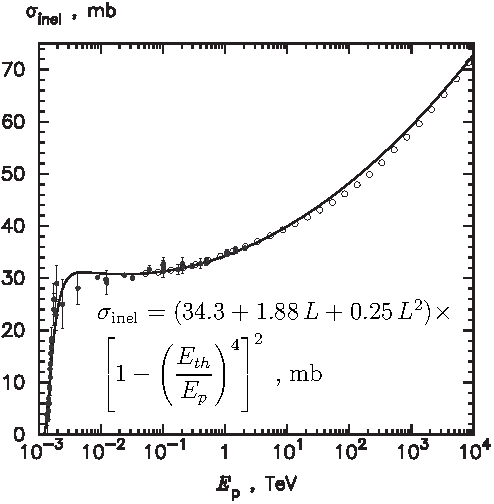
\includegraphics[width=0.5\textwidth]{figures/KelnerAharonian11.pdf}
\caption{Kelner Aharonian~\cite{Kelner2006prd}}
\end{figure}

The parametrization of experimental data for pion production in proton-proton collisions is detailed in~\cite{Norbury2009nimpb}:
%
\begin{eqnarray*}
\sigma_{pp\rightarrow \pi^+ X} & = & \left( 0.00717 + 0.0652 \frac{\log T_p}{T_p} + \frac{0.162}{T_p^2} \right)^{-1}~\text{mb} \\
\sigma_{pp\rightarrow \pi^- X} & = & \left( 0.00456 + \frac{0.0846}{T_p^{0.5}} + \frac{0.577}{T_p^{1.5}} \right)^{-1}~\text{mb} \\
\sigma_{pp\rightarrow \pi^0 X} & = & \left( 0.007 + 0.1 \frac{\log T_p}{T_p} + \frac{0.3}{T^2} \right)^{-1}~\text{mb} 
\end{eqnarray*}
%
where $T_p$ is the kinetic energy of the proton in the LAB frame in units of GeV.

An interesting characteristic of pion production is that the channels appear to follow the relation:
%
\[ 
\sigma_{pp\rightarrow \pi^0 X}  \simeq \frac{1}{2} (\sigma_{pp\rightarrow \pi^+ X}  + \sigma_{pp\rightarrow \pi^- X}) 
\]

\begin{figure}[t]
\centering
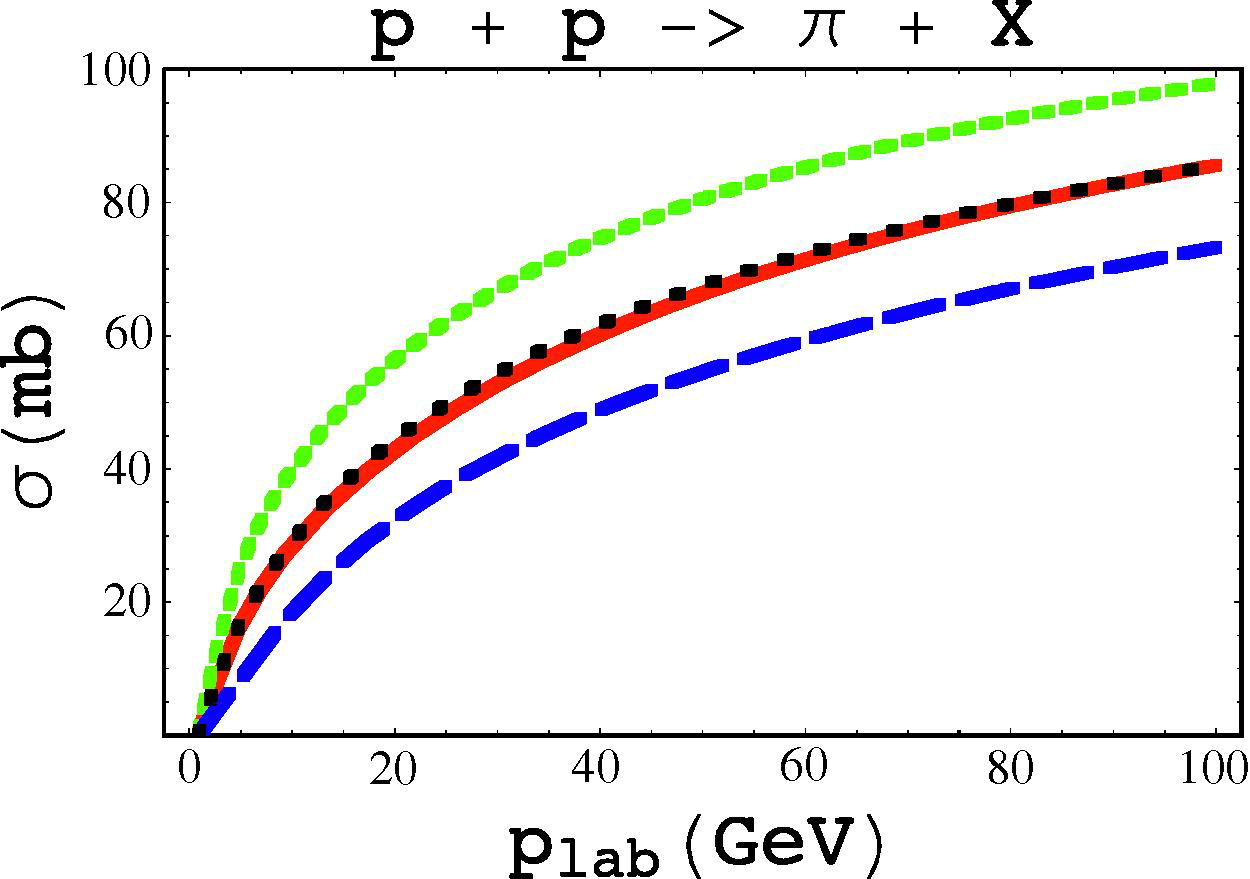
\includegraphics[width=0.5\textwidth]{figures/Norbury2009.jpg}
\caption{Parameterized inclusive cross sections for pion production in proton-proton collisions. The green dotted line is X. The red solid line is X. The blue long dashed line is X. The black dotted curve is calculated from X. ~\cite{Norbury2009nimpb}}
\end{figure}

It's noteworthy that the threshold for the \( p+p \rightarrow \pi^- + X \) reaction occurs at \( T_p \simeq 600 \) MeV, attributed to the presence of two new particles in the final state. This threshold is higher compared to the \( \pi^+ \) production, which has a threshold of \( T_b \simeq 289 \) MeV. This difference accounts for the consistently larger cross-section of \( \pi^+ \) compared to \( \pi^- \).

Consequently, this asymmetry in pion production leads to a greater secondary production of positrons than electrons in cosmic rays~\cite{Moskalenko1998apj}.

The inelasticity\footnote{The inelasticity is the fraction energy loss of the initial proton.} factor for this process, involving proton energies in the GeV-TeV range, is approximately \( K_{\pi^0} \simeq 0.17 \). Utilizing this value, we can derive the resulting spectrum from proton-proton (pp) interactions. For this purpose, we employ the delta-function approximation, expressed as \( T_\pi \simeq K_\pi T_p \).

We begin by introducing the pion emissivity as the number of pions produced per unit time, volume, and energy, denoted as \( q_\pi = \frac{dN_\pi}{dt dV dE} \). Consequently,
%
\[
q_\pi (E_\pi) = c n_{\rm H} \int \delta(T_\pi - K_\pi T_p) \sigma_{pp} (E_p) {N_p(E_p)} dE_p
\]
%
where...

Follows,
\[
q_\pi (E_\pi) \simeq c n_{\rm H} \int \delta(T_\pi - K_\pi E_p + K_\pi m_p) \sigma_{pp}(E_p) {N_p(E_p)} dE_p
\]
%
integrating over the $\delta$-function we arrive to
%
\[
q_\pi (E_\pi) \simeq \frac{c n_{\rm H}}{K_\pi} \sigma_{pp} \left(\frac{T_\pi}{K_\pi} + m_p \right) N_p \! \left(\frac{T_\pi}{K_\pi} + m_p \right)
\]

In the high-energy limit, where the mass of the pion can be disregarded,
%
\[
q_\pi (E_\pi) \underset{E_\pi \gg m_\pi}{\simeq} \frac{c n_{\rm H}}{K_\pi} \sigma_{pp}\left(\frac{E_\pi}{K_\pi}\right) N_p \! \left(\frac{E_\pi}{K_\pi} \right)
\]

As a result, the pion spectrum closely mirrors the shape of the parent proton spectrum, albeit shifted to a lower energy by a factor of \( K_\pi \).

\subsection{The $\pi^0$ gamma-ray spectrum}

The decay of \(\pi^0\) into two gamma photons occurs almost instantaneously. Due to momentum conservation, these photons are emitted in opposite directions (back-to-back) in the frame where the \(\pi^0\) is at rest (CoM). 
%
Energy conservation dictates that in this same frame, each photon carries an energy of \(E^\prime_\gamma = \frac{m_\pi}{2}\).

In the LAB frame, where the pion moves with velocity $\beta_\pi$,
%
\begin{equation}\label{eq:egamma}
E_\gamma = \frac{m_\pi}{2} \gamma_\pi (1+\beta_\pi \cos \theta^\prime)
\end{equation}
%
where $\theta^\prime$ is the angle between photons and the direction of the pion.

The minimum and maximum photon energies are determined by varying the angle \(\theta\) within its permissible range from -1 to 1:
%
\[
E_{\gamma}^{\rm min(max)} = \frac{m_\pi}{2} \gamma_\pi (1 \mp \beta_\pi)
\]

In the non-relativistic limit, where \(\beta \simeq 0\) and correspondingly \(\gamma \simeq 1\), both the minimum and maximum photon energies converge to \( E_{\gamma}^{\rm min} \simeq E_{\gamma}^{\rm max} \simeq \frac{m_\pi}{2} \).

Conversely, in the ultra-relativistic limit where \(\beta \simeq 1\) and \(\gamma \rightarrow \infty\), the minimum photon energy approaches \( E_\gamma^{\rm min} \simeq 0 \), while the maximum energy escalates to \( E_\gamma^{\rm max} \simeq E_\pi \rightarrow \infty \).

From Eq.~\ref{eq:egamma}, we deduce a relationship between the photon energy and the emission angle, leading to
%
\[
dE_\gamma = \frac{m_\pi}{2} \gamma_\pi \beta_\pi \, d\!\cos\theta^\prime
\]

Given that the pion is a scalar particle, its decay products are emitted isotropically. This is expressed as:
%
\[
\int d\Omega \frac{dN}{d\Omega} = 1 
\]
%
from this, we obtain~\footnote{Remind: $d\Omega = \sin \theta d\theta d\phi \rightarrow \langle d\Omega \rangle_\phi = 2 \pi d\cos\theta$}:
%
\[
\frac{dN}{d\Omega} = \frac{1}{4\pi} \rightarrow dN = \frac{1}{2} \, d\!\cos\theta^\prime
\]

Combined together, we conclude
%
\begin{remark}
\[
\frac{dN}{dE_\gamma} = \frac{1}{m_\pi \gamma \beta} = \frac{1}{(E^2_\pi - m_\pi^2)^{1/2}}
\]
\end{remark}

Therefore, after boosted for the energy of the emitting $\pi^0$, the probability to emit a photon of energy $E_\gamma$  is uniformly distributed in energy space between, in the relativistic limit, \(E_{\rm min} \simeq 0\) and \(E_{\rm max} \simeq E_\pi\). Essentially, one can expect a \emph{box-like} spectrum within this range.

We now move to calculate the mean energy using a logarithmic representation, that is:
%
\[
\langle \log E \rangle 
= \frac{1}{2} \left[ \log E_{\rm \gamma, min} + \log E_{\rm \gamma, max} \right] 
= \log \left[ \frac{E_\pi^2}{4} (1-\beta_\pi^2) \right]^{1/2} = \log \left(\frac{m_\pi}{2}\right)
\]

This implies that in a \emph{logarithmic scale}, the central point of the interval is equivalent to half the pion's rest mass, independent of \(E_\pi\).

The resulting spectrum is composed of a weighted sum of such \emph{box-like} distributions. Since each component of this distribution is symmetrically centered around \( m_\pi / 2 \), the photon distribution will peak at \( \log(m_\pi / 2) \).

Consequently, the gamma-ray spectrum consistently exhibits a prominent feature at approximately \( 67.5 \) MeV, regardless of the pion spectrum and, by extension, the spectrum of the parent protons.
%
A characteristic \emph{bump} in the energy spectrum, peaking at around $\sim$70 MeV, followed by a decline, might serve as a clear identifier of $\gamma$-rays originating from hadronic processes.

\begin{figure}[!t]
\centering
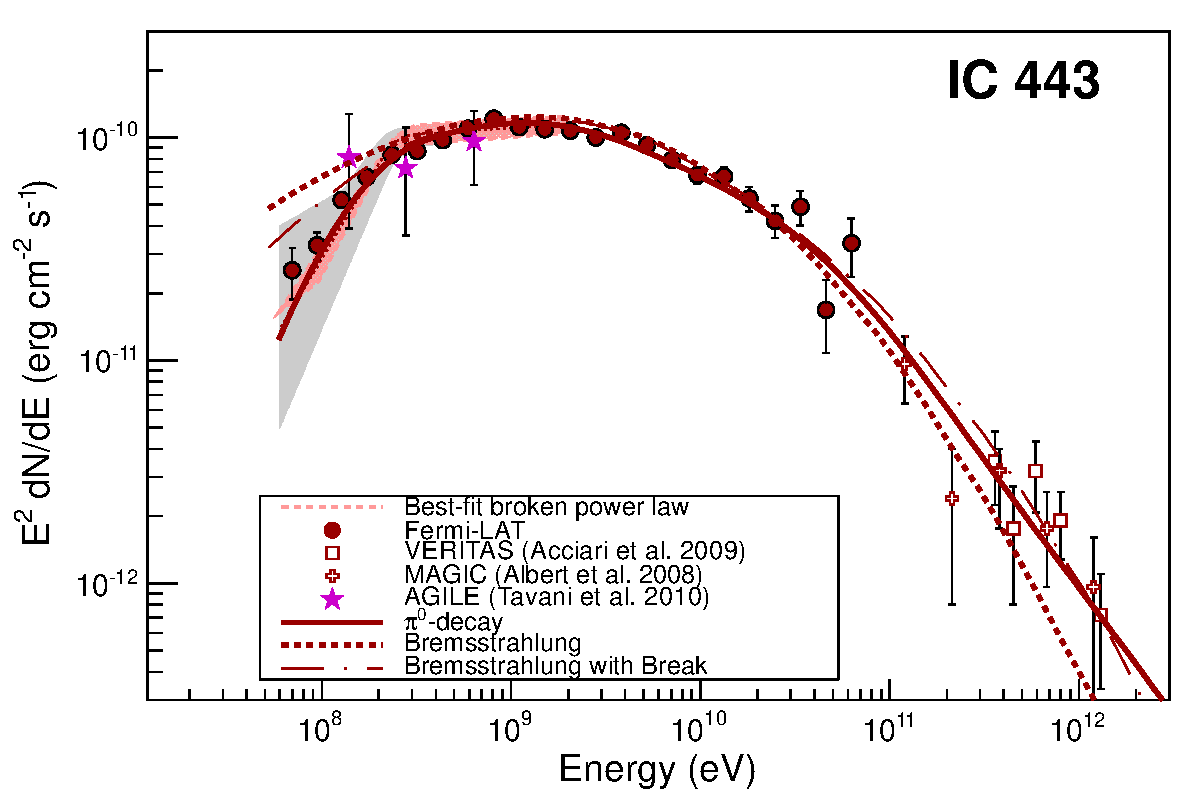
\includegraphics[width=0.45\textwidth]{figures/1231160fig2a.pdf}
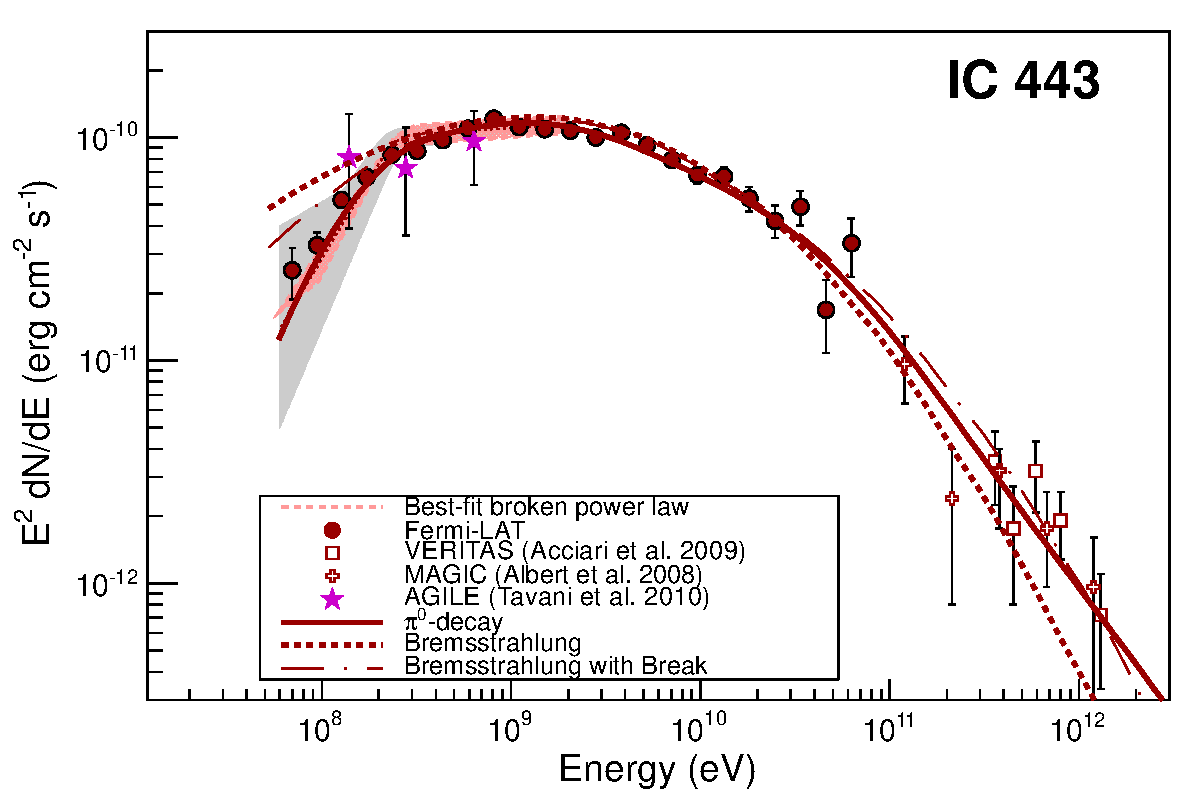
\includegraphics[width=0.45\textwidth]{figures/1231160fig2a.pdf}
\caption{In 2013 FERMI detected a feature compatible with the pion-bump in two old SNRs in interaction with Molecular Cloud~\cite{Ackermann2013sci}}
\end{figure}

Observe that \( E_{\rm \gamma, min} + E_{\rm \gamma, max} = E_\pi \) and \( E_{\rm \gamma, min} E_{\rm \gamma, max} = \frac{m_\pi^2}{4} \). Hence, we can express this as:
%
\[
E_\pi = E_{\rm \gamma, min} + E_{\rm \gamma, max} = E_{\rm \gamma, max} + \frac{m_\pi^2}{4E_{\rm \gamma, min}}
\]

As a result, for a given photon energy \( E_\gamma \), the minimum pion energy required to produce a photon of energy \( E_\gamma \) occurs when \( E_{\rm \gamma,min} = E_{\rm \gamma,max} = E_\gamma \), thereby:
%
\[
E_{\rm \pi, min} = E_\gamma + \frac{m_\pi^2}{4 E_\gamma}
\]

This relationship helps in determining the lower limit of the pion energy necessary for generating a photon of a specified energy \( E_\gamma \). In fact, the $\gamma$-ray emissivity can be written as
%
\[
q_\gamma(E_\gamma) = 2 \int_{E_{\rm \pi, min}}^\infty dE_\pi q(E_\pi) \frac{dN}{dE_\gamma} = 
2 \int_{E_\gamma + \frac{m_\pi^2}{4 E_\gamma}}^\infty dE_\pi \frac{q(E_\pi)}{(E_\pi^2 - m_\pi^2)^{1/2}} \simeq 2 \int_{E_\gamma}^\infty \frac{dE_\pi}{E_\pi} q_\pi(E_\pi)
\]
%
where the final expression holds true at very high energies, a regime in which the pion mass can be considered negligible.

Even at this early stage, we can note that the gamma-ray spectrum maintains the same spectral index as the protons, albeit shifted in energy by a factor of approximately \( K_\pi / 2 \).

To advance, let's calculate the pion emissivity as follows:
%
\[
q(E_\pi) = c n_{\rm H} \int_{E_\pi}^\infty dE_p N_p (E_p) \frac{d\sigma}{dE_\pi}(E_p, E_\pi)
\]
%
where $\frac{d\sigma}{dE_\pi}$ is the differential pion production cross section, $n_{\rm H}$ is the average matter density, \dots

The \emph{differential} cross-section for pion production in proton-proton interactions can be expressed in terms of the total inclusive cross-section as follows:
%
\[
\frac{d\sigma}{dE_\pi}(E_p, E_\pi) = \sigma_{pp}(E_p) \frac{f(E_p, E_\pi)}{E_\pi}
\]

Here, \(f\) is an auxiliary function designed to fit experimental data, fulfilling the condition $\int_{E_{\rm \pi,min}}^{E_{\rm \pi,max}} \frac{dE_\pi}{E_\pi} f(E_p, E_\pi) = 1$. 
%
Moreover, it has been observed that $f$ depends on \(E_p\) and \(E_\pi\) through the combined parameter \(x = E_\pi / E_p\). 

A parametrization of \(f(x)\) is provided in the literature~\cite{Cavasinni2006aph}:
%
\[
f(x) = 0.67 (1-x)^{3.5} + 0.5 \exp(-18 x)
\]

The proton intensity, as observed in cosmic radiation, is assumed to adhere to a power-law dependence on energy
%
\[
I_p(E_p) = I_0 \left(\frac{E_p}{E_0}\right)^{-\alpha}
\]

Upon substitution, the pion emissivity simplifies to
%
 \[
q(E_\pi) \simeq 4 \pi n_{\rm H} I_0 \sigma_0 \int_{E_\pi}^\infty \frac{dE_p}{E_\pi} \left(\frac{E_p}{E_0} \right)^{-\alpha} f(x) = 4 \pi n_{\rm H} I_0 \sigma_0 \left(\frac{E_\pi}{E_0} \right)^{-\alpha} \underbrace{ \int_0^1 dx x^{\alpha-2} f(x)}_{Y(\alpha)}
\]
%
where $Y(\alpha)$ is the spectrum-weighted yield of pions produced from a power-law proton spectrum of spectral index $\alpha$.

Finally, for a proton population following a power-law distribution, the photon emissivity can be expressed as:
%
\begin{remark}
\[
q(E_\gamma) = 2 \int_{E_\gamma}^\infty \frac{dE_\pi}{E_\pi} q(E_\pi) = 
8 \pi n_{\rm H} I_0 \sigma_0 Y(\alpha) \int_{E_\gamma}^\infty \frac{dE_\pi}{E_\pi}  \left(\frac{E_\pi}{E_0} \right)^{-\alpha}
= \frac{8 \pi}{\alpha} n_{\rm H}  \sigma_0 Y(\alpha) I_p\left(E_\gamma \right)
\]
\end{remark}

The final expression for \( q(E_\gamma) \) highlights the significant correlation between the spectral index of the proton energy spectrum and that of gamma rays, and by extension, with neutrinos:
%
\[
\alpha_p \simeq \alpha_\gamma \simeq \alpha_\nu
\]

In contrast to IC scattering, this relationship aids in differentiating between the two processes. Specifically, the gamma-ray spectrum resulting from hadronic processes more closely mirrors the spectral index of the parent protons, whereas gamma rays produced via IC scattering exhibit a comparatively flatter behavior relative to their parent electrons $E^{\frac{-\alpha-1}{2}}$.

\begin{problem}
Compute the shape of $q_\gamma(E_\gamma)$ using the fitting formula of Eq.~(1) in 1302.3307 and using the $\delta$-function approximation. Plot $q_\gamma(E_\gamma)$ in linear scale and $E_\gamma^2q_\gamma(E_\gamma)$ in log-log one. 
\end{problem}

To demonstrate the utility of these results, we estimate the expected diffuse galactic gamma-ray background, which arises from the scattering of cosmic rays through proton-proton interactions within our Galaxy.

Assuming the local cosmic rays are a fair representation of their overall density in the Galaxy, we can express the gamma-ray intensity as follows:
%
\[
I_\gamma(E_\gamma) = \frac{1}{4\pi} \int_{\rm los} \! ds \, q(E_\gamma) = \frac{2}{\alpha} N_{\rm H} \sigma_0 Y(\alpha) I_p(K_\gamma E_p) 
\]

Here, \( N_{\rm H} = \int_{\rm los} \! ds \, n_{\rm H} \) represents the column density of the gas, and \( K_\gamma = K_\pi / 2 \sim 0.1 \).

Consequently, the energy squared times the gamma-ray intensity is given by:
%
\[
E_\gamma^2 I_\gamma = \frac{2}{\alpha} N_{\rm H} \sigma_0 Y(\alpha) K_\gamma^2 \left[ E_p^2 I_p(E_p) \right]_{E_p = E_\gamma / K_\gamma}
\]

To calculate the gamma-ray intensity at 1 GeV, we utilize a gas column density along the Galactic plane of \( N_{\rm H} \simeq 10^{23} \) cm\(^{-2}\), as inferred from radio observations. The proton intensity, derived from direct measurements, is:
%
\[
\left[ E_p^2 I_p(E_p) \right]_{E_p = 10 \text{ GeV}} \simeq 2 \times 10^3 \text{ GeV m}^{-2} \text{s}^{-1} \text{sr}^{-1}
\]

Employing a cross-section \( \sigma_0 \simeq 30 \) mb, and {\color{red}a value of \( Y(\alpha) \) around 10}\footnote{Recompute...}, we find:
%
\[
E_\gamma^2 I_\gamma \simeq 5 \times 10^{-5} \text{ GeV cm}^{-2} \text{s}^{-1} \text{sr}^{-1}
\]

This estimate closely aligns with the average value of the diffuse emission measured around the Galactic plane (within \( |b| < 5.0 \) degrees) for \( E_\gamma \simeq \) GeV, for instance, by the Fermi-LAT.

This correlation strongly suggests that the diffuse galactic gamma-ray background is likely the result of pp interactions within our Galaxy.

%%% SUBSECTION %%%
\section{Nuclei-$\gamma$ Interactions}

In the vicinity of astrophysical sources, there is often a high density of photons spanning a range of wavelengths, including radio, infrared, visible, and ultraviolet.

While the cross-section for \(\gamma\)-proton interactions is typically two orders of magnitude smaller than that of pp interactions, in certain astrophysical environments, secondary meson production via photoproduction can be substantially higher than that from pp interactions. This increased probability is due to the much greater number density of ambient photons \(n_\gamma\) compared to the number density of matter in the environment.

In the interaction of nuclei with radiation fields, the dominant mechanism is photo-pion production, as exemplified by the following processes:
%
\[
p + \gamma \rightarrow \Delta^+ \rightarrow
\begin{cases} 
p + \pi^0 \\
n + \pi^+
\end{cases}
\]

The subsequent decay of these pions follows the same pattern as previously discussed.

At very high energies, multi-pion production becomes significant, represented by:
%
\[
p + \gamma \rightarrow p + a \pi^0 + b ( \pi^+ + \pi^-)
\]
%
where $a$ and $b$ are multiplicities...

For UHECRs, a competitive process for energy loss is pair production:
%
\[
p + \gamma \rightarrow p + e^+ + e^-
\]

The thresholds for these two processes can be calculated as:
%
\[
E_p^\pi = \frac{m_\pi^2 + 2 m_\pi m_p}{2 \epsilon (1 - \cos \theta)} \simeq 7 \times 10^9 \, \text{eV}
\]
and
\[
E_p^{ee} = \frac{4 m_e^2 + 8 m_e m_p}{2\epsilon (1 - \cos\theta)} \simeq 6 \times 10^{17} \, \text{eV}
\]

Notice that both energy thresholds are inversely proportional to \(\epsilon\). This implies that a lower energy threshold corresponds to interactions with a photon field of higher energy.

For pion production, the typical cross-section as measured in laboratory is:
%
\[
\sigma_{p\gamma} \simeq 
\begin{cases}
340 \, \mu\text{b} & 200 \, \text{MeV} \lesssim E^\prime_\gamma \lesssim 500 \, \text{MeV} \\
120 \, \mu\text{b} & E^\prime_\gamma \gtrsim 500 \, \text{MeV}
\end{cases}
\]

The inelasticity for the photo-pion production process is approximately \(K_{p\gamma} \simeq 0.2\).

Then, the cooling timescale associated with this process can be readily estimated as follows:
\[
t_c(E) \simeq \frac{E}{\dot E} \sim \frac{E}{\Delta E / \Delta t} \sim \frac{E}{K_{p\gamma} E} \frac{1}{n_\gamma c \sigma_{p\gamma}} = \frac{1}{K_{p\gamma} n_\gamma c \sigma_{p\gamma}}
\]

\subsection{Neutrinos from cosmic accelerators}

Various potential sources of ultra-high energy extragalactic cosmic rays are suggested as high-energy neutrino emitters. A prime example is GRBs, where the models for acceleration and neutrino production are closely aligned.

This relationship is used as a basis for estimating the expected upper limit of very high-energy neutrinos.

% The upper limit is determined as follows.

We start by assuming that the primary channels for HE pion production from hadronic interactions in extragalactic environments are p-$\gamma$ interactions, as previously discussed.

Due to isospin symmetry, the decay of the $\Delta^+$ resonance favors protons over neutrons, with branching ratios of 2/3 and 1/3, respectively. Correspondingly, similar processes involving neutrons instead of protons lead to the production of $\pi^-$ mesons.

As before, the average pion energy is \( \left\langle {E_\pi}/{E_p} \right\rangle \simeq \frac{1}{5} \).

Regardless of the specific process, both charged and neutral pions will decay in the following manner:
%
\begin{eqnarray*}
\pi^0 &\rightarrow& \gamma + \gamma \\
\pi^+ &\rightarrow& \nu_\mu + \mu^+ \rightarrow \nu_\mu + e^+ + \nu_e + \bar\nu_\mu 
\end{eqnarray*}

The energy inelasticities for these decay processes are as follows:
%
\begin{itemize}
\item For photons:
\[
\left\langle \frac{E_\gamma}{E_\pi} \right\rangle \simeq \frac{1}{2} \rightarrow \left\langle \frac{E_\gamma}{E_p} \right\rangle \simeq \frac{1}{10}
\]

\item And for neutrinos:
\[
\left\langle \frac{E_\nu}{E_\pi} \right\rangle \simeq \frac{1}{4} \rightarrow \left\langle \frac{E_\nu}{E_p} \right\rangle \simeq \frac{1}{20}
\]
\end{itemize}

These relationships clearly indicate that there must be a connection between UHECRs, neutrinos, and $\gamma$-rays.

An additional channel for neutrino production is through neutron decay, represented by the process:
%
\[
n \rightarrow p + e^- + \bar\nu_e
\]

However, neutrinos generated from neutron decay characteristically possess much lower energies, approximately on the order of \(10^{-2}\) times the energy of neutrinos produced from muon decays.

Consider \( Q_i(E) = \frac{dN}{dE \, dt} \) as the production rate of a particle type \( i \), representing the number of particles produced per unit time within the energy range \( E \) to \( E + dE \). From this, we can deduce:

For neutrinos:
\[
\sum_\alpha E_\nu Q_{\nu_\alpha}(E_\nu) = 3 \left[ E_{\pi^+} Q_{\pi^+} (E_{\pi^+}) \right]_{E_{\pi^+} \simeq 4 E_\nu}
\]

While for neutral pions:
\[
E_\gamma Q_\gamma(E_\gamma) \simeq 2 \left[ E_{\pi^0} Q_{\pi^0}(E_{\pi^0}) \right]_{E_{\pi^0} \simeq 2 E_\gamma}
\]

Assuming that \( E_{\pi^+} \simeq E_{\pi^0} \) and \( Q_{\pi^+} \simeq R_\pi Q_{\pi^0} \), the relationship between neutrino and gamma-ray production rates is given by:

\[
\frac{1}{3} \sum_\alpha E_\nu Q_{\nu_\alpha}(E_\nu) \simeq R_\pi \left[ E_{\pi^0} Q_{\pi^0} (E_{\pi^0}) \right]_{E_{\pi^0} \simeq 4 E_\nu}
\]

Therefore, we arrive at the relation:
%
\begin{remark}
\[
\frac{1}{3} \sum_\alpha E_\nu^2 Q_{\nu_\alpha}(E_\nu) \simeq \frac{R_\pi}{4} \left[ E^2_\gamma Q_{\gamma} (E_\gamma) \right]_{E_\gamma \simeq 2 E_\nu}
\] 
\end{remark}

This highlights the connection between photons and neutrinos.

Assuming a population of identical neutrino sources, each with a luminosity \(\mathcal L_\nu\) and a number density \(n_s\), the production rate per unit volume can be expressed as \(E^2\frac{dQ}{dV} \simeq \mathcal L_\nu n_s\). The resulting local neutrino intensity\footnote{See appendix...} is given by:
%
\[ E^2_\nu I_\nu \simeq \frac{c t_{\rm H}}{4\pi} \xi \mathcal L_\nu n_s \]

Here, \(t_{\rm H}\) represents the Hubble-Lemaître time, approximately equivalent to \(1/H_0\), and \(\xi_z \sim \mathcal O(1)\) is a factor that accounts for the redshift evolution of the sources.

IceCube has detected a diffuse neutrino emission characterized by an intensity of:
\[ E_\nu^2 I^{\rm IC}_\nu \simeq 2.8 \times 10^{-8} \, \text{GeV}~\text{cm}^{-2}~\text{s}^{-1}~\text{sr}^{-1} \]

Comparing this observed flux with our theoretical prediction allows us to establish an \emph{upper limit} for the properties of these neutrino sources:
%
\begin{remark}
\[
\mathcal L_\nu n_s \simeq \frac{4\pi}{\xi_z R_H} E_\nu^2 I^{\rm IC}_\nu \simeq 4 \times 10^{43}~\text{erg}~\text{Mpc}^{-3}~\text{yr}^{-1}  
\]
\end{remark}

In this equation, \(R_{\rm H} = c H_0^{-1} \simeq 4420\)~Mpc represents the current Hubble-Lemaître radius.

\begin{figure}[!t]
\centering
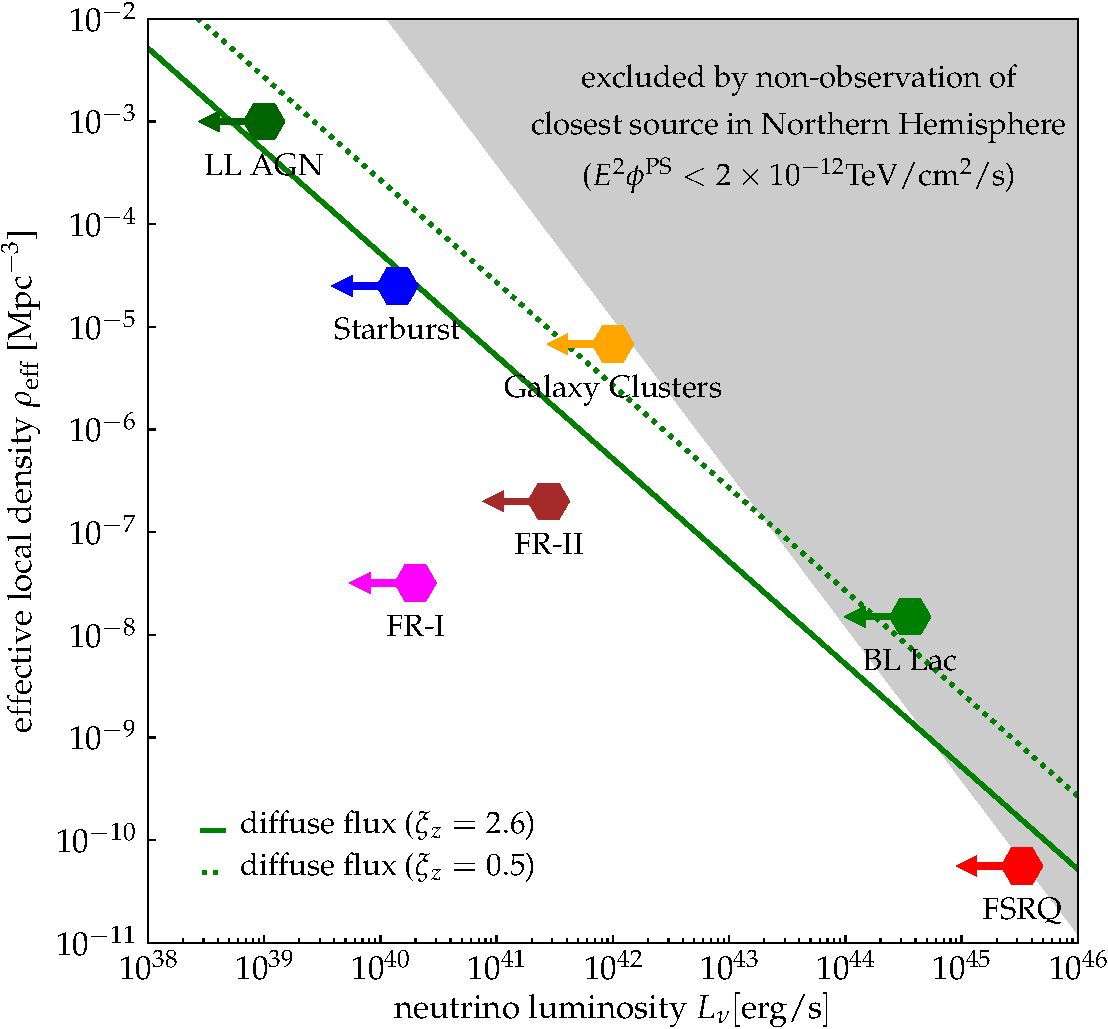
\includegraphics[width=0.5\textwidth]{figures/luminosityDISCOVERY.pdf}
\caption{Alhers Halzen~\cite{Ahlers2018ppnp}}
\end{figure}

Measurements of UHECRs have provided an estimated intensity at a proton energy of \(E_p \gtrsim 10^{17}\) eV as:
%
\[ 
E_p^2 I^{\rm UHE}_p \simeq 10^{-7} \, \text{GeV}~\text{cm}^{-2}~\text{s}^{-1}~\text{sr}^{-1} 
\]

Correspondingly, this implies a cosmic ray luminosity density of:
%
\[ 
E_p^2 \frac{dQ_p}{dV} \simeq 10^{44}~\text{erg}~\text{Mpc}^{-3}~\text{yr}^{-1} 
\]

Using these values, we can infer an upper limit for the production rate of pions:
%
\[
E_{\pi^+} Q_{\pi^+} (E_{\pi^+}) + E_{\pi^0} Q_{\pi^0}(E_{\pi^0}) \simeq \left[E_p Q_p(E_p) \right]_{E_p \simeq E_{\pi} \left\langle {E_p}/{E_{\pi}} \right\rangle}
\]

This relation can be approximated as:
\[
\left(\frac{1 + R_{\pi}}{R_{\pi}} \right) E_{\pi^+} Q_{\pi^+} (E_{\pi^+}) \simeq \left[E_p Q_p(E_p) \right]_{E_p \simeq E_{\pi} \left\langle {E_p}/{E_{\pi}} \right\rangle}
\]
And further refined to:
\[
\left(\frac{1 + R_{\pi}}{R_{\pi}} \right) E^2_{\pi^+} Q_{\pi^+} (E_{\pi^+}) \simeq \frac{1}{\left\langle {E_p}/{E_{\pi}} \right\rangle} \left[E^2_p Q_p(E_p) \right]_{E_p \simeq E_{\pi} \left\langle {E_p}/{E_{\pi}} \right\rangle}
\]

\begin{figure}[!t]
\centering
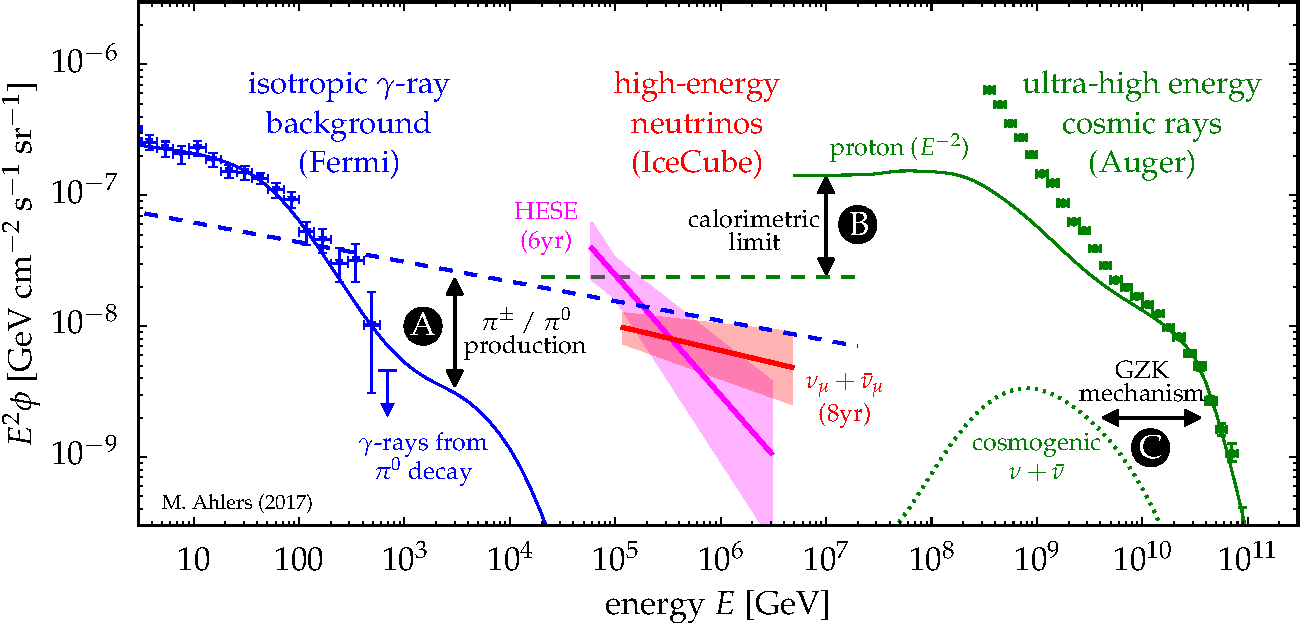
\includegraphics[width=0.90\textwidth]{figures/panorama.pdf}
\caption{Alhers Halzen~\cite{Ahlers2018ppnp}}
\end{figure}

Thus, the refined expression for the pion production rate becomes:
%
\begin{remark}
\[
E^2_{\pi^+} Q_{\pi^+} (E_{\pi^+}) \simeq x_{\pi} \frac{R_{\pi}}{1 + R_{\pi}}  \left[E^2_p Q_p(E_p) \right]_{E_p \simeq E_{\pi} \left\langle {E_p}/{E_{\pi}} \right\rangle}
\]
\end{remark}

Here, \(x_{\pi}\) denotes the average fraction of proton energy that gets converted into the energy of pions.

Integrating the previously derived equations, we obtain a relationship for the cumulative intensity of neutrinos across all flavors:
\[
\frac{1}{3} \sum_\alpha E_\nu^2 I_{\nu_\alpha} \lesssim 3 \times 10^{-8} x_\pi \left( \frac{\xi_z}{2.6} \right)~\text{GeV}~\text{cm}^{-2}~\text{s}^{-1}~\text{sr}^{-1}
\]
Here, \( f_\pi = 1 \) represents the calorimetric limit, also known as the Waxman-Bahcall bound. 

This upper limit is primarily applicable to transparent sources, as the local environment's opacity and the presence of other interaction processes, can also impact the overall neutrino production and escape mechanisms.. {\color{red}Say more...}

%, characterized as follows:
%
%In a transparent source scenario, protons are accelerated within regions containing strong magnetic fields. These protons interact with photons, leading to the generation of both neutral and charged pions. While secondary protons might be confined within the acceleration zone, approximately equal amounts of neutrons, as well as the decay products of both neutral and charged pions, escape. Consequently, the energy exiting the source is partitioned among cosmic rays, gamma rays, and neutrinos—the latter originating from the decay of neutrons, neutral pions, and charged pions.

An underlying assumption for this model is that the source spectrum is steeper than an \(E^{-2}\) energy distribution. This assumption is based on typical observations and theoretical considerations of cosmic ray sources. The steeper spectrum implies that there is a relatively higher abundance of lower-energy particles compared to the higher-energy ones, which influences the overall intensity and energy distribution of emitted particles, including neutrinos.

\newpage

\chapter{A Primer on Plasma Astrophysics}
% !TEX root = ../main.tex
\section{Ideal MHD}

{\color{red}TO BE DONE}


% !TEX root = ../main.tex
\section{Small Perturbations in a Plasma: MHD Waves}

MHD waves play a pivotal role in understanding the dynamics of astrophysical plasmas. In this section, we explore the concept of small perturbations in a plasma under the framework of ideal MHD, characterized by infinite conductivity. This assumption is particularly relevant in astrophysical contexts, where the presence of electric fields is minimal.

We start by listing the fundamental equations governing the behavior of such plasmas and subsequently analyze them in the context of small perturbations, drawing parallels with the analysis of sound waves.

\begin{enumerate}
\item The mass conservation equation, representing the conservation of mass in the plasma, is given by:
%
\begin{equation}
\frac{\partial \rho}{\partial t} + \nabla \cdot (\rho \vb{v})=0
\end{equation}
where \(\rho\) is the plasma density, and \(\vb{v}\) is the velocity field.

\item The momentum conservation equation, reflecting the balance of forces in the plasma, is:
%
\begin{equation}
\rho \frac{\partial \vb{v}}{\partial t} + \rho \vb{v} \cdot \nabla \vb{v} = - \nabla P + \frac{1}{4\pi} (\nabla \times \vb{B}) \times \vb{B}
\end{equation}
%
where \(P\) is the pressure, and \(\vb{B}\) is the magnetic field.

\item The adiabaticity condition ensures constant entropy in the system (see appendix):
%
\begin{equation}\label{eq:adiabatic}
\left[ \frac{\partial}{\partial t} + \vb{v}\cdot \vb{\nabla} \right] \frac{P}{\rho^\gamma}=0
\end{equation}

\item The induction equation, under the assumption of infinite conductivity, is:
%
\begin{equation}
\frac{\partial \vb{B}}{\partial t}=\nabla \times (\vb{v}\times\vb{B})
\end{equation}
This equation leads to the concept of flux freezing in the plasma, a phenomenon where magnetic field lines are \emph{frozen} into the plasma and move with it.

\item Finally, the divergence-free nature of the magnetic field is expressed as:
\begin{equation}
{\nabla}\cdot\vb{B}=0
\end{equation}
\end{enumerate}

We assume a background unperturbed stationary state of the plasma given by:
%
\begin{equation}
\rho = \rho_0 \, , \,\,\, P = P_0 \, , \,\,\, \vb{v} = 0 \, , \,\,\, \vb{B} = B_0 \hat{\vb{z}}
\end{equation}

In this state, the magnetic field \(\vb{B}_0\) is ordered and aligned along the z-axis, i.e., \( \vb{B}_0 \equiv (0,0,B_0) \), and the plasma is considered at rest in the reference frame \( \vb{v}_0 = 0 \)~.

As for the sound wave case, we introduce perturbations in these quantities, which can be decomposed into Fourier modes. This approach simplifies the analysis by breaking down complex wave patterns into simpler components. Each quantity is assumed to have the form:
%
\[
\delta A \, {\rm e}^{-i\omega t + i \vb{k} \cdot \vb{x}}
\]

Our goal is to derive a dispersion relation \( \mathcal F (k, \omega) = 0 \) for the allowed modes in the system.

By linearizing the motion equations and discarding second-order perturbations or higher, we obtain:
%
\begin{eqnarray}
-i \omega \delta \rho + i \rho_0 \vb{k} \cdot \delta \vb{v} & = & 0 \label{eq:dmhd1}\\ 
-i \omega \rho_0 \delta \vb{v} & = & - i \vb{k} \delta P + \frac{i}{4\pi} \left(\vb{k} \times \delta \vb{B} \right) \times \vb{B}_0  \label{eq:dmhd2}\\
-i \omega \delta P \rho^{-\gamma} + i\omega P \gamma \rho^{-\gamma-1}\delta \rho & = & 0 \label{eq:dmhd3}\\
-i \omega \delta \vb{B} & = & i \vb{k} \times \left( \delta \vb{v} \times \vb{B}_0  \right) \label{eq:dmhd4}\\ 
\vb{k} \cdot \delta \vb{B} & = & 0  \label{eq:dmhd5}
\end{eqnarray}

Equation (\ref{eq:dmhd5}) implies that for all modes, the wave vector \( \vb{k} \) is perpendicular to the perturbation in the magnetic field, i.e. \( \vb k \perp \delta \vb{B} \).

Equation (\ref{eq:dmhd3}) can be expressed as:
%
\begin{equation}
\frac{\delta P}{\delta \rho}=\frac{\gamma P_0}{\rho_0} \equiv c_s^2
\end{equation}
%
illustrating that in terms of pressure and density perturbations the plasma behaves as sound hydro-waves.

%Therefore we can rewrite \eqref{2pert} using both \eqref{1pert} and \eqref{3pert}
%\begin{equation}
%\begin{cases}
%\delta P =c_s^2\delta \rho\\
%\delta \rho=\frac{\rho}{\omega} \vec{k}\cdot \delta \vec{v}
%\end{cases}
%\end{equation}
%\begin{equation}
%\implies \delta P =c_s^2\frac{\rho}{\omega} \vec{k}\cdot \delta \vec{v}
%\end{equation}
%Remember that we want to rewrite all the perturbations in terms of one only

Now, substituting the derived expressions for perturbations into Eq.~\ref{eq:dmhd2}, we obtain an equation for \( \delta \vb{v} \) only:
%
\begin{equation}
-i \omega \rho \delta \vb{v} = -i \vb{k} c_s^2 \frac{\rho}{\omega}(\vb{k} \cdot \delta \vb{v}) - \frac{i}{4\pi \omega} \left[ \vb{k} \times \left(\vb{k}\times\left( \delta \vb{v} \times \vb{B}_0 \right)  \right) \right] \times \vb{B}_0
\end{equation}
%
which simplifies to:
%
\begin{equation}
\delta \vb{v} = 
\frac{c_s^2}{\omega^2} \vb{k} (\vb{k} \cdot \delta \vb{v}) 
+ \frac{1}{4\pi \rho \omega^2} \left[ \vb{k} \times \left(\vb{k}\times\left( \delta \vb{v} \times \vb{B}_0 \right)  \right) \right] \times \vb{B}_0
\end{equation}

This allows us to solve for \( \delta \vb{v} \) and subsequently derive all other perturbed quantities.

Considering the simplifying assumption \(\vb{k} \parallel \vb{B}_0\), we have \(\vb{k}=(0,0,k)\). This leads to:
%
\begin{equation}
\left[ \vb{k} \times \left[\vb{k} \times \left(\delta \vb{v} \times \vb{B}_0  \right) \right] \right] \times \vb{B}_0 = 
\begin{pmatrix}
k^2 B_0^2 \delta v_x\\
-k^2 B_0^2 \delta v_y\\
0
\end{pmatrix}
\end{equation}

From this, we can express the perturbations as:
\begin{equation}
\begin{pmatrix}
\delta v_x\\
\delta v_y\\
\delta v_z
\end{pmatrix} = \frac{k^2 c_s^2}{\omega^2} \begin{pmatrix}
0\\
0\\
\delta v_z
\end{pmatrix}+ \frac{k^2B_0^2}{4\pi \rho\omega^2} \begin{pmatrix}
\delta v_x\\
\delta v_y\\
0
\end{pmatrix}
\end{equation}

This leads to the distinction between oscillations:
%
\begin{itemize}
\item For parallel oscillations (\(\delta v_z\)), we find sound waves with the dispersion relation:
%
\begin{equation}
\omega^2 = c_s^2 k^2
\end{equation}
%
\item For perpendicular oscillations (\(\delta v_x, \delta v_y\)), we find Alfvén waves with:
\begin{equation}
\omega^2=\frac{k^2B_0^2}{4\pi \rho}
\end{equation}
\end{itemize}
%
These Alfvén waves are characterized by the relation:
%
\begin{remark}
\begin{equation}
\omega^2 = v_A^2 k^2
\end{equation}
\end{remark}
%
where the Alfvén velocity \( v_A \) is defined as \( v_A=\frac{B_0}{\sqrt{4\pi \rho}} \).

In summary, perturbing a magnetized fluid with parallel perturbations (\( \vb{k} \parallel \vb{B}_0 \)) results in two types of waves: sound waves moving parallel to \(\vb{B}_0\) and Alfvén waves moving perpendicular to \(\vb{B}_0\).

We are considering now the case when \( \vb{k} \perp \vb{B}_0$, in particular we assume \(  \vb{k}=(k,0,0) \)~.

The nested vector products calculation simplifies to:
%
\begin{equation}
\left[ \vb{k} \times \left[\vb{k} \times \left(\delta \vb{v} \times \vb{B}_0 \right) \right] \right] \times \vb{B}_0 = 
\begin{vmatrix}
\hat{x} & \hat{y} & \hat{z} \\
0 & k^2B_0 \delta v_x & 0 \\
0 & 0 & B_0
\end{vmatrix} = \begin{pmatrix}
k^2 B_0^2 \delta v_x\\
0 \\
0
\end{pmatrix}
\end{equation}

This leads to the following expression for the perturbations:
%
\begin{equation}
\begin{pmatrix}
\delta v_x\\
\delta v_y\\
\delta v_z
\end{pmatrix} = \frac{c_s^2 k^2}{\omega^2} 
\begin{pmatrix}
\delta v_x\\
0 \\
0
\end{pmatrix} 
+ \frac{k^2 B_0^2}{4\pi\rho}
\begin{pmatrix}
\delta v_x\\
0\\
0
\end{pmatrix}
\end{equation}

This result indicates that the transported perturbations are parallel to the \(\hat{x}\) axis. From this, we can derive the following relation for the velocity of these perturbations:
%
\begin{equation}
v^2 = c_S^2 + v_A^2
\end{equation}

This equation reveals that the speed of \emph{magnetosonic} modes is a combination of the sound speed (\(c_S^2\)) and the Alfvén speed (\(v_A^2\)). Magnetosonic modes, therefore, represent a unique type of wave in ideal MHD, characterized by their dependence on both the fluid's sound speed and the magnetic field's Alfvén speed.

In conclusion, in unmagnetized fluids, small perturbations propagate isotropically as sound waves. The introduction of a magnetic field into the system not only increases the diversity of possible wave modes but also introduces anisotropy to wave propagation, which now becomes dependent on the orientation relative to the magnetic field. 

Moreover, the presence of a magnetic field induces an electric field in the Galactic frame, perpendicular to both \(\vb{B}_0\) and \(\delta \vb{v}\). In the context of Alfvén waves, this induced electric field possesses a strength on the order of \(\frac{v_A}{c} B_0\), which is small for most astrophysical plasmas. This electric field plays a pivotal role in the so-called \emph{second-order Fermi re-acceleration}, a mechanism where charged particles gain energy in a stochastic manner through interactions with these weak electric fields (see section~X).

%%% END CGPT

%So a charged particle in a plasma will experience the following motions:
%\begin{itemize}
%\item
%helicoidal motion for $\vec{B}_0$
%\item
%motion because of $\delta \vec{B}$
%\item
%interaction with the induced electric field $\vec{E}$
%\end{itemize}
% !TEX root = ../main.tex
\section{Charged Particle Motion in Turbulent Magnetic Fields}
\label{app:diffusioncoefficient}

Here we explore the interaction between a charged particle and an astrophysical plasma to derive the spatial diffusion coefficient using the quasilinear theory (QLT). 
%
QLT allows to directly compute this coefficient and other transport parameters based on the previous knowledge of the turbulent spectra.
%
The quasilinear approximation can be seen as a first-order perturbation theory and here we follow standard derivations as in~\cite{Blandford1987pr,Shalchi2009book,Blasi2013aar}.

First, we consider the equations of motion for a particle traveling within an ordered magnetic field aligned with the $\hat{\vb z}$ axis, denoted as $\vb B_0 = B_0 \hat{\vb z}$. In the absence of a large-scale electric field, the particle's motion is described by the Lorentz force:
%
\begin{equation}
\frac{d \vb p}{dt} = \frac{q}{c} (\vb v \times \vb B_0)
\label{eq:lorentz}
\end{equation}

The Lorentz force acts perpendicular to the particle's motion, preserving the velocity's magnitude (see appendix). By splitting the motion into its components, we obtain:
%
\begin{equation}
m \gamma \frac{d \vb v}{dt} = \frac{q}{c} (\vb v \times \vb B_0) \quad \rightarrow \quad 
\begin{cases}
m \gamma \frac{dv_x}{dt} = \frac{q}{c} v_y B_0 \\
m \gamma \frac{dv_y}{dt} = -\frac{q}{c} v_x B_0\\
\frac{dv_z}{dt} = 0
\end{cases}
\label{eq:lorentzcomponents}
\end{equation}

The last equation shows that $v_z = v_\| = v \cos \theta$ remains constant. Consequently, the pitch angle, defined as the cosine of the angle between the particle velocity and the magnetic field direction ($\mu = \cos \theta$), is a conserved quantity, as $dv_z/dt = v d\mu/dt = 0$.

Combining the first two equations yields two second-order differential equations:
%
\begin{equation}
\frac{d^2 v_{x,y}}{dt^2} = - \Omega^2 v_{x,y}
\end{equation}

Here, we introduce the Larmor frequency 
\begin{equation}
\Omega = \frac{q B_0}{m \gamma c} \simeq 10^{-2} Z \left(\frac{B_0}{\rm \mu G}\right) \left(\frac{E}{\rm GeV}\right)^{-1}~\text{rad}~\text{s}^{-1}
\end{equation}

{\color{red}Introduce here the Larmor radius...}

This equation can be easily solved as simple harmonic motion along the $\hat{\vb x}$ axis, where $v_{x} = v_{0,x} \cos (\Omega t)$. Using this solution, we can solve the system~\eqref{eq:lorentzcomponents} as follows:
%
\begin{equation}
\begin{cases}
v_x = v_{0,\perp} \cos (\phi - \Omega t) \\
v_y = - v_{0,\perp} \sin (\phi - \Omega t) \\
v_z = v_{0,\parallel}
\end{cases}
\rightarrow \, 
\begin{cases}
v_x = v_{0} (1 - \mu^2)^{\frac{1}{2}} \cos (\phi - \Omega t) \\
v_y = - v_{0} (1 - \mu^2)^{\frac{1}{2}} \sin (\phi - \Omega t) \\
v_z = v_{0} \mu
\end{cases}
\end{equation}

Here, $\phi$ is an arbitrary phase, $v_{0,\perp}$ represents the initial velocity of the particle in the $xy$-plane, given by $v_{0,\perp} = v_0 \sin \theta = v_0 (1-\mu^2)^{1/2}$.

The solution above represents a helical motion with a uniform drift along $\hat{\vb z}$, described by the equation of motion $z = v \mu t$.

Now we consider introducing a perturbation to the magnetic field with components $\delta \mathbf{B} \equiv (\delta {\rm B}_x, \delta {\rm B}_y, \delta {\rm B}_z)$, where $|\delta \mathbf{B}| \ll |\mathbf{B}_0|$. In this case, we assume a pure Alfvénic wave propagating along the background magnetic field, which implies $\delta {\rm B}_z = 0$ and the wave oscillates such that $\delta \mathbf{B} \perp \mathbf{k}$.

This allows us to express the system of equations~\eqref{eq:lorentz} as follows:
%
\begin{equation}
m \gamma \frac{d\vb v}{dt} = \frac{q}{c}
\left(
\begin{array}{ccc}
\hat {\vb x}  & \hat {\vb y}  & \hat {\vb z}  \\
v_x & v_y & v_z \\
\delta {\rm B}_x & \delta {\rm B}_y & {\rm B}_0 
\end{array}
\right)
\oset{\delta {\rm B} \ll {\rm B}_0} \simeq
\frac{q}{c}
\left(
\begin{array}{c}
v_y {\rm B}_0 \\
-v_x {\rm B}_0 \\
v_x \delta {\rm B}_y - v_y \delta {\rm B}_x
\end{array}
\right)
\end{equation}

As prescribed by QLT, we neglect the perturbation field in the $x$ and $y$ components. This implies that the circular orbits in the plane perpendicular to the background field are approximately unaffected. However, the perturbation does cause a change in the $z$ component of the velocity, leading to a modification in the pitch angle $\mu$ of the particle. It's important to note that the perturbation does not affect the particle's momentum value; we are describing the motion in the reference frame of the perturbation, where the only force acting on the particle is the Lorentz force. Consequently, while numerous pitch-angle changes can eventually reverse the parallel velocity of the particle, they cannot shift the guiding center of the orbits.

To examine the extent of this change, we focus on the last equation of the system mentioned above, which governs the \emph{perturbed} motion along $z$:
%
\begin{equation}
m \gamma \frac{dv_z}{dt} = \frac{q}{c} \left[v_x(t) \delta {\rm B}_y - v_y(t) \delta {\rm B}_x \right]
\end{equation}

As a consequence, the pitch angle changes with time according to:
%
\begin{equation}
m\gamma v \frac{d\mu}{dt} = \frac{q}{c}v_{0,\perp} \left[\cos(\phi-\Omega t) \delta {\rm B}_y - \sin(\phi - \Omega t) \delta {\rm B}_x\right]
\label{eq:pitchanglemotion}
\end{equation}

To proceed, we make the simplifying assumption that the perturbed field is circularly polarized, meaning the wave components have the same amplitude: $|\delta {\rm B}_{x}| = |\delta {\rm B}_{y}| = |\delta {\rm B}|$. Thus, we can express the perturbation as:
%
\begin{equation}
\begin{cases}
\delta {\rm B}_y = &  \delta {\rm B} \exp \left[ i (kz - \omega t) \right] \\ %= \cos(kz - \omega t + \psi) + i \sin ((kz - \omega t + \psi)\\
\delta {\rm B}_x = & \pm i \delta {\rm B}
\end{cases}
\end{equation}

Taking the real part gives:
%
\begin{equation}
\begin{cases}\delta {\rm B}_y = & \delta {\rm B} \cos (kz - \omega t) \\
\delta {\rm B}_x = & \mp\delta {\rm B} \sin (kz - \omega t) 
\end{cases}
\end{equation}
%
therefore, by substituting in equation~\eqref{eq:pitchanglemotion}, we find
%
\begin{equation}
m\gamma v \frac{d\mu}{dt} = 
\frac{q}{c}v_{0,\perp} \delta{\rm B} \left[\cos(\phi-\Omega t) \cos (kz - \omega t) \pm \sin(\phi - \Omega t) \sin (kz - \omega t)\right]
\end{equation}
%
which simplifies to\footnote{We use the trigonometric relation $\cos \alpha \cos \beta \pm \sin \alpha \sin \beta = \cos (\alpha \pm \beta)$}:
%
\begin{equation}
m\gamma v \frac{d\mu}{dt} = 
\frac{q}{c}v_{0,\perp} \delta {\rm B} \cos(\phi-\Omega t \mp kz \pm \omega t)
\end{equation}

For Alfvén waves, the dispersion relation is given by $\omega = k v_{\rm A}$, where $v_{\rm A}$ represents the Alfvén velocity. By comparing the spatial frequency with the temporal frequency in the argument of the cosine function, we can derive the following relation:
%
\begin{equation}
\frac{kz}{\omega t} \simeq \frac{k v \mu t}{k v_{\rm A} t} \sim \frac{v}{v_{\rm A}} \mu
\label{eq:kmomegat}
\end{equation}

Here, we utilize the fact that for an unperturbed orbit, the position $z$ of the particle is given by $z = v \mu t$.

Considering that $v$ is on the order of the speed of light, while $v_{\rm A}$ in the average ISM is approximately 10 km/s, we find that the ratio in equation~\eqref{eq:kmomegat} is significantly greater than 1 unless $\mu \ll v_{\rm A} / v$.

Consequently, we can neglect the term $\omega t$ in comparison to $kz$. This choice is equivalent to selecting a reference frame in which the waves appear stationary. In this frame, there is no electric field associated with the waves.

We can approximate the pitch angle equation of motion as
%
\begin{equation}
\frac{d\mu}{dt} \simeq \Omega
(1-\mu^2)^{\frac 1 2} \frac{\delta {\rm B}}{{\rm B}_0} \cos\left[\phi + (\Omega \pm k v \mu) t \right]
\end{equation}

The equation above implies a periodic variation in the pitch angle. When we integrate this equation over a sufficiently long time interval, the average of the integrated quantity becomes zero. This result is physically expected since the particle orbits are concentric circles.

However, if we instead consider the square of the pitch-angle variation: 
%
\begin{multline}
\langle \Delta \mu \Delta \mu \rangle = \int_0^{2\pi} \frac{d\phi}{2\pi} \int_0^{\Delta t} dt \frac{d\mu}{dt}(t) \, \int_0^{\Delta t} dt^\prime \frac{d\mu}{dt}(t^\prime) \\ = \Omega^2 (1 - \mu^2) \left( \frac{\delta {\rm B}}{{\rm B}_0} \right)^2 \int_{0}^{\Delta t} dt \int_{0}^{\Delta t} dt^\prime \, \cos[(\Omega \pm k v \mu) t] \cos[(\Omega \pm k v \mu) t^\prime]
\end{multline}

The integrand functions are even, so we can double the interval of the $dt^\prime$ integral as $\int_{-\Delta t}^{\Delta t} dt^\prime$ and add a factor of $\frac{1}{2}$. Additionally, as we are considering sufficiently large times to evaluate the effect of scattering ($\Delta t \gg t, t^\prime$), the same interval can be approximated as $\int_{-\infty}^{\infty} dt^\prime$.

Therefore, we have\footnote{We are grateful to A.~Marcowith for providing clarification on this passage.}:
%
\begin{multline}
\langle \Delta \mu \Delta \mu \rangle = \\ \Omega^2 \frac{(1 - \mu^2)}{2} \left( \frac{\delta {\rm B}}{{\rm B}_0} \right)^2 \int_{0}^{\Delta t} \!\! dt \, {\rm Re} \{ \exp[i(\Omega \pm k v \mu) t] \} \, \int_{-\infty}^{\infty} \!\! dt^\prime \,  {\rm Re}\{\exp[i(\Omega \pm k v \mu) t^\prime]\}
\end{multline}
%
and solve the integral on $t^\prime$\footnote{We use the property $\delta(x-a) = \frac{1}{2\pi}\int_{-\infty}^\infty dy {\rm e}^{iy(x-a)}$}, as to obtain:
%
\begin{equation}
\langle \Delta \mu \Delta \mu \rangle = \Omega^2 \frac{(1 - \mu^2)}{2} \left( \frac{\delta {\rm B}}{{\rm B}_0} \right)^2 \int_{0}^{\Delta t} \!\! dt \, {\rm Re} \{ \exp[i(\Omega \pm k v \mu) t] \} \, 2\pi \delta (\Omega \pm k v \mu)
\end{equation}

Now the second integral, because of the presence of the~\emph{delta} function, gives just a factor $\int_{0}^{\Delta t} dt = \Delta t$, and we find:
%
\begin{equation}
D_{\mu\mu} \equiv \left\langle \frac{\Delta \mu \Delta \mu}{\Delta t} \right\rangle = \Omega^2 \left( \frac{\delta {\rm B}}{{\rm B}_0} \right)^2 (1 - \mu^2) \, \pi \delta(\Omega \pm k v_{\parallel})
\label{eq:dmumuvar}
\end{equation}
%
where $D_{\mu \mu}$ represents the average rate of change of the square of the pitch angle over the time interval $\Delta t$.

We see that on average \( \mu \) remains constant, but its variance linearly grows with time: This is the typical behaviour of a \emph{diffusive} process (see appendix).

In general, one must consider a packet of turbulent waves with energy distribution per wave number denoted as $W(k) dk$. This distribution represents the energy density contained within the range of wavenumbers $[k, k + dk]$ and is normalized to the energy density of the background magnetic field, \( \frac{B_0^2}{8\pi} \). Specifically:
%
\begin{equation}
\left( \frac{\delta {\rm B}(k)}{{\rm B}_0} \right)^2 = W(k) dk.
\end{equation}

By incorporating this consideration, we can extend equation~\eqref{eq:dmumuvar} to obtain:
%
\begin{equation}
D_{\mu \mu} \equiv \left\langle \frac{\Delta \mu \Delta \mu}{\Delta t} \right\rangle = \Omega^2 (1 - \mu^2) \pi \int dk \, W(k) \delta(\Omega \pm k v_{\parallel}) \, .
\end{equation}

Introducing the resonant wavenumber \( k_{\rm res} \), defined as the inverse of the Larmor radius \( k_{\rm res} = r_{\rm L}^{-1} = \Omega v_\| \), we can express $D_{\mu \mu}$ as follows\footnote{We use the property $\int dx \delta (c x) = \frac{1}{|c|} \int dx \delta (x)$}:
%
\begin{equation} 
D_{\mu \mu} = \Omega (1 - \mu^2) \pi k_{\mathrm{res}} \int dk \, W(k) \delta(k \pm k_{\mathrm{res}}) = \Omega (1 - \mu^2) \pi k_{\mathrm{res}} W(k_{\rm res})
\end{equation}

These equations reveal that a wave-particle interaction is only possible when the inverse Larmor radius of the particle matches (i.e., is resonant) with the wavenumber of the turbulent wave (modulo a geometric projection). 
%
This type of process is commonly referred to as \emph{gyroresonant} scattering\footnote{It is worth noting that the QLT is consistently inadequate when attempting to describe pitch-angle diffusion at 90 degrees ($\mu = 0$) and reversing direction becomes a consideration. To address these and other limitations, several Nonlinear Theories have been formulated and developed.}.

The typical diffusion time, defined as the timescale to invert the pitch angle by about one radian is
%
\begin{equation}
\tau_{\rm diff} \simeq \frac{1}{D_{\theta\theta}} = \frac{1-\mu^2}{D_{\mu\mu}} = \frac{1}{\pi \Omega k_{\rm res} W(k_{\rm res})}
\end{equation}
%
where $D_{\theta\theta}$ is the diffusion coefficient in angle.

As in a diffusion timescale the particle moves by a distance of about $\Delta z = v \tau_{\rm diff}$, the spatial diffusion coefficient coefficient can be roughly estimated as
%
\begin{equation}
D_{zz} \simeq v (v \tau_{\rm diff}) = \frac{v^2}{\pi \Omega k_{\rm res} W(k_{\rm res})} \simeq \frac{1}{3} r_{\rm L} v \frac{1}{k_{\rm res} W(k_{\rm res})} = D_{\rm B} \frac{1}{k_{\rm res} W(k_{\rm res})}
\end{equation}
%
which informs us that the spatial diffusion coefficient is always much larger than the Bohm diffusion (\( D_{\rm B} \)) since \( k_{\rm res} W(k_{\rm res}) \ll 1 \) as a consequence of QLT proposition.

{\color{red}Consequences for Galactic transport...}

The spectral density \( W(k) \) exhibits a power-law behavior within the so-called \emph{inertial} range, spanning from an outer scale (characterized by low \( k \), signifying the injection scale of turbulence) to a smaller scale (with large \( k \), where dissipative effects become significant).

In a turbulence regime where \( W(k) \) is proportional to \( k^{-\alpha} \), the spatial diffusion coefficient \( D_{zz} \) displays a dependency on rigidity \( R \) that follows the relation \( D_{zz} \propto R^{2-\alpha} \).

A classical turbulence model, influenced by hydrodynamic principles, is the \emph{Kolmogorov} model. It is characterized by \( \alpha = 5/3 \), leading to a rigidity dependence of the diffusion coefficient expressed as \( D_{zz} \propto R^{1/3} \). This model reflects a scenario where smaller eddies are successively generated from larger ones in a cascading process.

On the other hand, the \emph{Kraichnan} model, another well-established theory in turbulence, suggests \( \alpha = 3/2 \). In this framework, \( D_{zz} \) shows a different rigidity dependency, following the relation \( D_{zz} \propto R^{1/2} \). This model is indicative of a more rapid energy transfer across scales compared to the Kolmogorov model.

{\color{red}What happens when \( \mu \rightarrow 0 \) or when \( k_{\rm res} > k_0 \)?}

% !TEX root = ../lectures.tex
\section{The Advection-Diffusion Equation}

Consider a beam of particles exhibiting a range of pitch angles. We aim to understand the evolution of this beam due to resonance effect introduced before. 
%
The transport equation that we obtain will bridge the gap between microphysics and macrophysics in this context.

The key quantity here is the phase-space density, \( f = f (\vb x, \vb p, t) \), defined so that the number \( d N \) of particles at time \( t \) is a given phase-space volume element is
%
\[
f \equiv \frac{dN}{d^3 \vb x d^3 \vb p}
\]

Note that \( f \) is relativistic invariant, since both the number of particles and the phase-space element {\color{red}(see appendix)} are relativistic invariants.

 To streamline our analysis, we make the following assumptions:
%
\begin{equation}
f(\vb{x}, \vb{p}, t) \rightarrow f(z, \mu, t)
\end{equation}
%
Here, the motion is predominantly in the \( z \) direction, Alfv\'en waves are stationary (thereby keeping \( |p| \) constant), and azimuthal symmetry is assumed (making \( \mu \) the relevant angle).

\subsection{The Diffusion Equation in Pitch Angle}

We aim at describing the evolution of the function \( f \) over a time interval \( \Delta t \):
%
\begin{equation}
f(z, \mu, t) \rightarrow f(z + v\mu\Delta t,\mu, t + \Delta t)
\end{equation}

To facilitate this, we introduce \(\Psi(\mu, \Delta \mu)\), a function representing the likelihood of a particle altering its angle by an amount \( \Delta\mu \)~. 
%
This probability obeys the integral constraint:
%
\begin{equation}\label{eq:normpsi}
\int \Psi(\mu, \Delta\mu) d\Delta\mu = 1, \quad \forall \mu
\end{equation}

Thus, the evolved function can be expressed as an integral over all potential variations of \( \Delta \mu \) leading to \( \mu \): 
%
\begin{equation}\label{eq:distribpert}
f(z + v\mu\Delta t, \mu, t+\Delta t) = \int d\Delta \mu f(z, \mu-\Delta\mu, t) \Psi(\mu-\Delta\mu, \Delta\mu)
\end{equation}

Assuming small variations, we apply perturbation theory and perform a second-order Taylor expansion.

For the LHS:
%
\begin{equation}
f(z+v\mu\Delta t,\mu, t+\Delta t)=f+\frac{\partial f}{\partial z} v\mu \Delta t+\frac{\partial f}{\partial t} \Delta t
\end{equation}

For the RHS, we consider:
%
\begin{equation}
f(z,\mu-\Delta\mu,t)=f-\frac{\partial f}{\partial \mu}\Delta\mu +\frac{1}{2}\frac{\partial^2 f}{\partial \mu^2}\Delta\mu\Delta\mu 
\end{equation}
%
and
%
\begin{equation}
\Psi(\mu-\Delta\mu,\Delta\mu)=\Psi -\frac{\partial \Psi}{\partial \mu}\Delta\mu +\frac{1}{2}\frac{\partial^2 \Psi}{\partial \mu^2}\Delta\mu\Delta\mu 
\end{equation}

Inserting these into equation~\eqref{eq:distribpert} and retaining only terms up to second order, we obtain:
%
\begin{equation}\label{eq:fwithawithb}
\frac{\partial f}{\partial t} \Delta t  +  v \mu \frac{\partial f}{\partial z} \Delta t = 
-\frac{\partial}{\partial \mu} \left( \mathcal A f \right) + \frac{1}{2} \frac{\partial^2}{\partial\mu^2}\left(\mathcal B f \right)
\end{equation}

Here, we have used that:
%
\begin{equation}
\frac{\partial^2}{\partial\mu^2}\left(\Psi f\right) = \frac{\partial^2 f}{\partial\mu^2} \Psi +2\frac{\partial f}{\partial\mu}\frac{\partial\Psi}{\partial\mu}+f\frac{\partial^2 \Psi}{\partial\mu^2}
\end{equation}
%
and we have defined the mean value of \( \Delta\mu \) as:
%
\begin{equation}
\mathcal A(\mu) \equiv \int d\Delta\mu \Delta\mu \Psi
\end{equation}
%
and the variance as:
%
\begin{equation}
\mathcal B(\mu) \equiv \int d\Delta\mu \Delta\mu\Delta\mu \Psi
\end{equation}

Let's integrate the concept of \emph{detailed balance} into our analysis, applying it to the probability distribution \(\Psi\):
%
\begin{equation}
\Psi(\mu, -\Delta\mu ) = \Psi(\mu-\Delta\mu , \Delta\mu )
\end{equation}

%This property of detailed balance ensures equilibrium in reversible processes. 

By Taylor expanding this expression, we further elucidate its implications:
%
\begin{equation}\label{eq:detbalexp}
\Psi(\mu, -\Delta\mu ) = \Psi(\mu-\Delta\mu , \Delta\mu )=\Psi(\mu,\Delta\mu )-\frac{\partial \Psi}{\partial \mu} \Delta\mu +\frac{1}{2}\frac{\partial^2 \Psi}{\partial\mu^2} \Delta\mu^2
\end{equation}

Integrating equation~\eqref{eq:detbalexp} over \(d\Delta\mu\) and using the general property in equation~\eqref{eq:normpsi}:
%
\begin{equation}
-\frac{\partial}{\partial \mu} \left( \int d\Delta\mu \Psi \Delta\mu \right) + \frac{1}{2}\frac{\partial^2}{\partial\mu^2}\left( \int d\Delta\mu \Delta\mu^2 \Psi \right) = \cancelto{1}{\int d\Delta\mu \Psi(\mu, -\Delta\mu )} - \cancelto{1}{\int d\Delta\mu \Psi(\mu,\Delta\mu)} = 0
\end{equation}
%
we recognize that we can write as:
%
%\begin{equation}
%-\frac{\partial \mathcal A}{\partial \mu} + \frac{1}{2} \frac{\partial^2 \mathcal B}{\partial\mu^2} = 0 
%\end{equation}
%
\begin{equation}
\frac{\partial}{\partial\mu}\left[ \mathcal A-\frac{1}{2}\frac{\partial \mathcal B}{\partial \mu}\right] = 0
\end{equation}

It implies that the quantity \( \mathcal A - \frac{1}{2} \frac{\partial \mathcal B}{\partial \mu} \) must be a \emph{constant} with respect to \( \mu \).  

We compute explicitly the derivative of \( \mathcal B \) with respect to \( \mu \) as
%
\begin{equation}
\frac{\partial B}{\partial \mu} = \frac{\partial}{\partial\mu} \int d\Delta\mu \Delta\mu\Delta\mu \Psi(\mu,  \Delta\mu)
=   \int d\Delta\mu \Delta\mu\Delta\mu \frac{\partial}{\partial\mu} \Psi(\mu,  \Delta\mu)
\end{equation}

By invoking the principle of detailed balance again, we obtain:
%
\begin{equation}
\frac{\partial\Psi}{\partial\mu}(\mu,\Delta\mu) = \frac{\partial\Psi}{\partial\mu}(\mu-\Delta\mu,\Delta\mu)=\frac{\partial\Psi}{\partial\mu}(\mu+\Delta\mu ,-\Delta\mu)
\end{equation}

We introduce a new variable \( \mu^\prime = \mu+\Delta\mu \), which leads to \( \Delta\mu = \mu^\prime -\mu \) and:
%
\begin{equation}\label{eq:newmuequation}
\frac{\partial\Psi}{\partial\mu}(\mu,\Delta\mu) = \frac{\partial\Psi}{\partial\mu}(\mu^\prime, \mu - \mu^\prime) = -\frac{\partial}{\partial \Delta\mu} \Psi(\mu+\Delta\mu, -\Delta\mu)
\end{equation}

Incorporating this into the definition of $\frac{\partial B}{\partial \mu}$ and using equation~\ref{eq:newmuequation}, we find:
%
\begin{equation}
\frac{\partial \mathcal B}{\partial \mu} = 2 \mathcal A
\end{equation}

Substituting this back into the equation~\ref{eq:fwithawithb} governing \( f \), we arrive at:
%
\begin{equation}
\frac{\partial f}{\partial t} \Delta t  +  v \mu \frac{\partial f}{\partial z} \Delta t = 
\Delta t \frac{\partial}{\partial\mu} \left[D_{\mu\mu}\frac{\partial f}{\partial\mu}\right]
\end{equation}

Here, the RHS includes the pitch angle diffusion coefficient, representing a \emph{collision term}:
%
\begin{equation}
D_{\mu\mu} \equiv \frac{1}{2}\langle \frac{\Delta\mu\Delta\mu}{\Delta t}\rangle = \frac{1}{2} \int d \Delta\mu \frac{\Delta\mu\Delta\mu}{\Delta t} \Psi
\end{equation}

This leads us to understand how the distribution \( f \) evolves due to pitch angle diffusion:
%
\begin{remark}
\begin{equation}\label{eq:fdiffmu}
\frac{\partial f}{\partial t} +v\mu \frac{\partial f}{\partial z} = \frac{\partial}{\partial\mu}\left[D_{\mu\mu}\frac{\partial f}{\partial\mu}  \right]
\end{equation}
\end{remark}

We have formulated a Fokker-Planck equation that characterizes the distribution's pitch angle diffusion over time, influenced by Alfvén waves present in the plasma. This equation exemplifies typical diffusive processes, where the variance of the distribution increases proportionally with time.

Crucially, the term \( D_{\mu\mu} \) in the equation represents a form of \emph{collision} term. However, unlike conventional collisions involving atoms, this term describes the effect of scattering due to Alfvén waves. 

The diffusion coefficient \( D_{\mu\mu} \), encapsulating the microphysical interactions, is computed for a background of Alfvén waves and is proportional to \( (1-\mu^2) F(k, p) \). This formula reflects the nuanced interplay between the pitch angle \( \mu \) and the wave-particle dynamics.

Given this dynamic, we expect the particle distribution to become isotropic over time, especially in the reference frame of the Alfvén waves. This isotropization signifies a uniform distribution of particle velocities in all directions, relative to the wave frame.

To transition from pitch angle diffusion to spatial diffusion, we consider the inherent nature of diffusive processes, which strive to make any system as isotropic as possible. In the context of Alfvén waves, this isotropization leads to a residual anisotropy proportional to the ratio of the Alfvén speed (\( v_A \)) to the speed of light (\( c \)). This outcome illustrates the profound impact of diffusion in a plasma, where cosmic rays, typically near light-speed, collectively move at the slower Alfvén speed.

After establishing diffusion, we assume the distribution \( f \) in phase space becomes isotropic, with a slight anisotropy represented as:
%
\[
f = M + f_1 \mu
\]

Here, \( f_1 \mu \) corresponds to the anisotropy, a dipole effect induced by the motion of the Alfvén waves relative to the observer's frame of reference. This anisotropy is a subtle yet significant manifestation of the dynamic interaction between particles and the wave environment in a plasma.

\subsection{The Diffusion Equation in Space}

Now, we shift our focus from pitch angle diffusion to spatial diffusion. We consider the case where the function \( f \) is only weakly dependent on the pitch angle \(\mu\). In fact, we found that such a distribution is expected to become \emph{isotropized} by the scattering with waves, moreover the anisotropy observed in cosmic rays is \( \sim 10^{-4} \) at all energies.

To transition from pitch angle distribution to spatial diffusion, we apply the operator \(\frac{1}{2}\int_{-1}^{1} d\mu\) to all terms of equation~\eqref{eq:fdiffmu}. We also introduce a new definition:
%
\begin{equation}\label{eq:Mdef}
M = \frac{1}{2}\int_{-1}^1 d\mu \, f(\mu)
\end{equation}

Notice that if \( f \) remains constant with respect to \( \mu \), then \( M \) simplifies to \( f \) itself. Essentially, \( M \) extracts the isotropic component of \( f \).

Upon applying this operator, we derive:
%
\begin{equation}
\frac{\partial M}{\partial t} +\frac{v}{2}\frac{\partial}{\partial z}\int_{-1}^1 d\mu \, \mu f= \left[ {D_{\mu\mu}\frac{\partial f}{\partial \mu}} \right]_{-1}^{1} \simeq 0
\end{equation}

This result emerges because the diffusion coefficient \( D_{\mu\mu} \) is proportional to \( (1-\mu^2) \). Moreover, as \( f \) becomes isotropic, the term \( \frac{\partial f}{\partial \mu} \) tends towards zero as well. 

Let's introduce a new term to represent the flux of particles (i.e., a current):
%
\begin{equation}\label{eq:defj}
\frac{1}{2}\int_{-1}^1 d\mu \, v\mu f = J
\end{equation}

With this in mind, the evolution of \( M \) can be expressed as:
%
\begin{equation}\label{eq:jmcont}
\frac{\partial M}{\partial t} + \frac{\partial J}{\partial z} = 0
\end{equation}

This equation implies that changes in \( M \) over time are directly linked to the spatial gradients of the current, \( J \). In other words, \( M \) evolves over time only if there is a corresponding change in the current.

Now, let's focus on the current \( J \) itself:
%
\begin{equation}
J 
= \frac{1}{2} v\int_{-1}^1 d\mu \, f\mu  
= -\frac{v}{4}\int_{-1}^1 d\mu \, f\frac{\partial}{\partial \mu}(1-\mu^2) 
\end{equation}
%
hence
%
\begin{equation}\label{eq:jpartialmu}
J = \cancel{\left[ -\frac{v}{4}(1-\mu^2)f \right]_{-1}^{+1}} + \frac{v}{4}\int_{-1}^{+1} d\mu \, (1-\mu^2) \frac{\partial f}{\partial \mu}
\end{equation}

The equation leverages the identity \(\mu = -\frac{1}{2}\frac{\partial}{\partial \mu}(1-\mu^2)\), a mathematical manipulation that simplifies the expression.

By integrating this equation from \( -1 \) to \( \mu \), we get:
%
\begin{equation}
\frac{\partial}{\partial t}\int_{-1}^{\mu} d\mu' f +\int_{-1}^{\mu} d\mu' v\mu' \frac{\partial f}{\partial z}=D_{\mu\mu}\frac{\partial f}{\partial \mu}
\end{equation}

Multiplying this equation by \( \frac{1-\mu^2}{D_{\mu\mu}} \) and assuming that \( f \) is isotropic in all quantities where \( \mu \) does not appear explicitly, we obtain:
%
\begin{equation}
(1-\mu^2)\frac{\partial f}{\partial \mu}=\frac{1-\mu^2}{D_{\mu\mu}} \frac{\partial M}{\partial t}(1+\mu) + v\frac{\partial M}{\partial z}\frac{1}{2} (\mu^2-1)\frac{(1-\mu^2)}{D_{\mu\mu}}
\end{equation}

Further integrating this equation over \( \mu \), we derive:
%
\begin{equation}
\int_{-1}^{+1} d\mu (1-\mu^2)\frac{\partial f}{\partial \mu} =\frac{\partial M}{\partial t}\int_{-1}^{+1} d\mu \frac{(1-\mu^2)}{D_{\mu\mu}}(1+\mu) -\frac{1}{2}v\frac{\partial M}{\partial z}\int_{-1}^{+1} d\mu \frac{(1-\mu^2)^2}{D_{\mu\mu}}
\end{equation}

Using equation~\eqref{eq:jpartialmu}, we find the expression for the current \( J \):
%
\begin{equation}
J = \frac{v}{4}\frac{\partial M}{\partial t}\int_{-1}^{+1} d\mu \frac{(1-\mu^2)}{D_{\mu\mu}}(1+\mu) -\frac{v^2}{8}\frac{\partial M}{\partial z}\int_{-1}^{+1} d\mu \frac{(1-\mu^2)^2}{D_{\mu\mu}}
\end{equation}

We introduce two new quantities, \( K_t \) and \( K_z \), defined as:
%
\begin{equation}
K_t \equiv \frac{v}{4} \int_{-1}^{+1}d\mu \frac{(1-\mu^2)(1+\mu)}{D_{\mu\mu}} 
\end{equation}
\begin{equation}\label{eq:kzz}
K_z \equiv \frac{v^2}{8}\int_{-1}^{+1} d\mu \frac{(1-\mu^2)^2}{D_{\mu\mu}}
\end{equation}

Finally, applying these to equation \eqref{eq:jmcont}, we reach the following conclusion:
%
\begin{equation}
\frac{\partial M}{\partial t} = \frac{\partial }{\partial z}\left[ K_t\frac{\partial J}{\partial z} + K_z\frac{\partial M}{\partial z}  \right]
\end{equation}

%%%% END CGPT %%%%

We can estimate the magnitudes of the terms in the diffusion equation:
%
\begin{equation}
K_t \frac{\partial J}{\partial z}\sim \frac{v}{D_{\mu\mu}}\frac{J}{z}
\end{equation}
\begin{equation}
K_z\frac{\partial M}{\partial z} \sim \frac{v}{D_{\mu\mu}}\frac{vM}{z}
\end{equation}

Based on the definition in equation~\eqref{eq:defj}, we can express the current \( J \) as follows:
%
\begin{equation}
J = \frac{1}{2} \int_{-1}^1 d\mu \, v\mu f \simeq \frac{1}{2} \int_{-1}^1 d\mu \, v\mu (f_0 + \mu f_1) 
\end{equation}

Here, \( f_1 \ll f_0 = M \) due to the near-isotropic nature of the distribution function, allowing for a linear expansion.

This leads us to:
%
\begin{equation}
J = \frac{v}{2} \left[ f_0 \cancel{\int_{-1}^1 d\mu \, \mu} + f_1 \int_{-1}^1 d\mu \, \mu^2 \right] \sim v f_1 \ll v M
\end{equation}

Since \( f_1 \) is much smaller than \( f_0 \), this implies that \( J \) is significantly smaller than \( vM \).

With these considerations, in good approximation, we can write an equation for the time evolution of the isotropic component of the distribution function, \( M \), as:
%
\begin{remark}
\begin{equation}
\frac{\partial M}{\partial t} \simeq \frac{\partial}{\partial z}\left[K_z \frac{\partial M}{\partial z}  \right]
\end{equation}
\end{remark}

The equation we have derived is a classic \emph{diffusion equation}, where \( K_z \), as defined earlier, acts as the spatial diffusion coefficient. This equation is determined by the diffusion coefficient \( K_z \), which is intricately linked to the probability distribution function \( \Psi \). By understanding \( \Psi \), one can deduce \( K_z \), thereby establishing a connection between microphysical interactions and their macroscopic implications.

In this context, the diffusive flux \( J \) is expressed as \( J = -K_z \frac{\partial M}{\partial z} \). This formulation allows us to compute the current from the distribution function \( M \), considering it as a first-order correction to the particle flux. 

This dynamic emerges from the somewhat inhomogeneous nature of the function \( f \). It's the gradient of \( f \) that generates a net current, driving the evolution of the isotropic component \( M \) over time. The gradient effectively causes a net transport of particles, leading to changes in the distribution \( M \) in response to spatial inhomogeneities.

\subsection{The Diffusion Equation in Space with Moving Plasma}

{\color{red}To be done}

\newpage

\chapter{The Physics of Galactic Sources}
% !TEX root = ../lectures.tex
\section{Small Perturbations in a Fluid: Sound Waves}

In fluid dynamics, we often encounter scenarios where disturbances in the fluid are \emph{small} compared to the equilibrium values of a steady state solution. 
%
Consider a fluid at equilibrium with a density \(\rho_0(x)\) at a given point. If a disturbance occurs at time \(t\), altering the density to \(\rho(x, t)\), we define the relative density difference as \( \frac{\delta \rho}{\rho} = \frac{\rho(x, t) - \rho_0(x)}{\rho_0(x)} \). 
%
We assume that a linear theory can be developed as long as this relative difference remains  \( \frac{\delta \rho}{\rho} \ll 1 \).

The validity of linear theory allows us to \emph{linearize} the equations of motion around the equilibrium state. This simplification transforms the complex, non-linear fluid dynamics equations into more manageable linear differential equations. These linear equations are advantageous as they adhere to the superposition principle, making the analysis and solution of these disturbances more straightforward.

Within this linear framework, the disturbances propagate as a series of normal modes. Each mode represents a wave with a distinct frequency. Any arbitrary disturbance in the fluid can thus be reduced to a linear superposition of these fundamental wave modes. 

However, it is crucial to note that certain conditions might lead to one or more normal modes exhibiting exponential growth over time. In such scenarios, even infinitesimal perturbations can amplify beyond the linear theory's scope, rendering the linear approximation invalid. This exponential growth is indicative of an \emph{instability} in the fluid's equilibrium state.

To descrive the dynamics of small perturbations, we revisit the fundamental fluid equations. 
%
The conservation law for any physical quantity \(A\) in fluid dynamics is generally expressed as:
%
\[
\frac{\partial}{\partial t} (\text{density of}~A) + \nabla \cdot (\text{flux of}~A) = 0
\]
%
This equation encapsulates the principle that any change in the density of \(A\) over time must be compensated by the divergence of its flux. Source and sink terms are included on the right-hand side if they are present in the system.

In this context, we are adopting the \emph{Eulerian} perspective, which focuses on describing physical quantities at fixed spatial locations  over time. 
%
Accordingly, the temporal change of a quantity \(A\) in the Eulerian perspective is described by the partial time derivative:
%
\[
\frac{\partial A}{\partial t} = \frac{A(\vb x, t +\delta t) - A(\vb x, t)}{\delta t} 
\]

In contrast, the \emph{Lagrangian} view offers a different approach, emphasizing tracking physical quantities as they move with the fluid flow. This perspective is akin to following a fluid parcel as it travels through space and time. Here, the temporal changes in a quantity \(Q\) are described by a convective time derivative:
%
\[
\frac{d A}{dt} = \frac{A(\vb x + \delta \vb x, t + \delta t) - A(\vb x, t)}{\delta t} 
\]
%
where \( \delta \vb x \) is the displacement, which can be expressed as \( \vb v \delta t \), with \( \vb v \) being the velocity of the fluid element.

To transition from the fixed fluid element description (Lagrangian) to a fixed position in space description (Eulerian), we use the relation:
%
\begin{equation}
\frac{d}{dt} \rightarrow \frac{\partial}{\partial t} + \vb u \cdot \nabla
\end{equation}

To describe the dynamics of a fluid, we introduce these quantities that are functions of both space and time: density (\( \rho \)), velocity (\( \vb v \)), and pressure (\( P \)).

The continuity equation reflects the principle of mass conservation in fluid dynamics:
%
\begin{equation}
\frac{d\rho}{dt}  = 0 \rightarrow \frac{\partial \rho}{\partial t} + \nabla \cdot (\rho \vb v) = 0
\end{equation}

The Euler equation describes the conservation of momentum in the fluid:
%
\begin{equation}
\frac{\partial \vb v}{\partial t} + \vb v \cdot \nabla \vb v = - \frac{\nabla P}{\rho}
\end{equation}

This equation relates the variation of momentum density (\( \rho \vb v \)) to the gradient of pressure (which act a net force on the system).
%
Additional forces, like gravity (represented through its potential by \( - \nabla \phi \)), can be included on the RHS.

To solve the continuity and Euler equations, the relationship between pressure and other fluid properties must be established. This is where the equation of state (EoS) becomes essential.

In the case of a barotropic fluid, a common simplification in fluid dynamics, the EoS is expressed as \( P=P(\rho) \). This relationship directly relates pressure to density, providing a way to close the system of equations.

For more complex scenarios, where the EoS also depends on temperature, an additional equation governing the evolution of temperature is necessary. 

\TODO{See appendix on hydrostatic. TBD}

Consider a fluid in a static steady state defined by a constant density \( \rho_0(x) \), pressure \( P_0(x) \), and zero velocity \( \vb v_0(x) = 0 \). This state, being time-independent, will persist indefinitely in the absence of external disturbances.

Now, let's introduce small perturbations into this system, denoted by \( \delta A \), where \( A \) represents the fluid properties, and we assume the relative perturbation to be \( \delta A / A \ll 1 \). 

These perturbations lead to changes in the fluid's velocity, density, and pressure:
%
\begin{eqnarray}
\vb v = 0 & \rightarrow & \vb v = \delta \vb v \\
\rho = \rho_0 & \rightarrow & \rho = \rho_0 + \delta \rho \\
P = P_0 & \rightarrow & P = P_0 + \delta P
\end{eqnarray}

With these perturbations, the continuity equation is modified as:
%
\begin{equation}
\frac{\partial}{\partial t} \delta \rho + \rho_0 \nabla \cdot \delta \vb v = - \nabla \cdot ( \cancel{\delta \rho \delta \vb v}) \simeq 0
\end{equation}

Similarly, the Euler equation for the perturbed state becomes:
%
\begin{equation}
\frac{\partial}{\partial t} \delta \vb v = -\cancel{\delta \vb v \cdot \nabla \delta \vb v} - \frac{1}{\rho_0 + \cancel{\delta \rho}} \nabla \delta P \simeq - \frac{\nabla \delta P}{\rho_0} 
\end{equation}

In both cases, we simplified the equations by linearizing them, which involves discarding higher-order terms and using the equations valid for the background state. Specifically, we eliminate the non-linear term \( \vb v \cdot \nabla \vb v \), which often complicates or renders problems unsolvable and is a primary factor in modeling \emph{turbulence} within fluid equations.

Now, we focus exclusively on adiabatic perturbations, wherein the entropy remains constant. Under this condition, the variation in pressure, typically a function of density \( \rho \) and entropy \( s \), can be expressed as:
%
\begin{equation}
\delta P = \left( \frac{\partial P}{\partial \rho} \right)_s \delta \rho + \left( \frac{\partial P}{\partial s} \right)_\rho \delta s \simeq \left( \frac{\partial P}{\partial \rho} \right)_s \delta \rho \equiv c_{s,0}^2 \delta \rho
\end{equation}

Here, \( c_{s,0}^2 \equiv  \left( \frac{\partial P}{\partial \rho} \right)_s \) is considered a constant. In particular, for an equation of state \( P = K \rho^\gamma \), the constant is given by 
\begin{equation}\label{eq:cs02}
c_{s,0}^2 = \frac{\gamma P_0}{\rho_0}~.
\end{equation}

Moving forward, by differentiating the continuity equation with respect to time and using the Euler equation, we can combine the two to derive:
%
\begin{equation}
\frac{\partial^2}{\partial t^2} \delta \rho - \nabla^2 \delta P = 0
\end{equation}

Finally, applying the equation of state, we arrive at:
%
\begin{remark}
\begin{equation}
\frac{\partial^2}{\partial t^2} \delta \rho - c_{s,0}^2 \nabla^2 \delta \rho = 0
\end{equation}
\end{remark}

This equation is a hyperbolic partial differential equation, commonly known as the \emph{wave equation}. 
%
Indeed, the general solution of this equation is in the form of:
%
\begin{equation}
\delta \rho = R(x - c_{s,0} t) + L (x + c_{s,0} t)
\end{equation}

Here, \( R \) and \( L \) are arbitrary functions representing disturbances propagating to the right and left, respectively, at a velocity \( c_{s,0} \), which turns our to be the speed of sound in the medium.

Given that the problem is both linear and homogeneous, the solution to the wave equation can be effectively found using \emph{eigenmode} decomposition. This approach allows us to break down any disturbance into a series of Fourier modes, each of which can be solved independently.

For each mode characterized by a wavenumber \( k \), we seek solutions in the following form:
%
\begin{equation}
\delta \rho = \rho_0 A {\rm e}^{i(\vb k \cdot \vb x - \omega t)}
\end{equation}

Here, \( A \) represents a constant amplitude, with the condition \( A \ll 1 \) ensuring that the perturbations remain small.

We can demonstrate that any function \( f \) of this type satisfies the following relations:
%
\begin{eqnarray}
\frac{\partial^2}{\partial t^2} f & = & - \omega^2 f \\
\nabla^2 f & = & -k^2 f
\end{eqnarray}

Consequently, we derive from the wave equation that the condition for the existence of non-trivial solutions is:
%
\begin{remark}
\begin{equation}
\omega^2 - c_{s,0}^2 k^2 = 0
\end{equation}
\end{remark}

This condition effectively establishes a \emph{dispersion relation}, indicating that for a given medium with a sound speed of \( c_{s,0} \), the frequency of the wave is directly proportional to its wavenumber. 

Reverting to the original form of the perturbation and taking the real part\footnote{Recall Euler's formula \( e^{ix} = \cos x + i \sin x \).}, the solution for a single mode propagation is expressed as:
%
\begin{equation}\label{eq:rhowaveform}
\frac{\delta \rho}{\rho_0} = A \cos(kx + \omega t) + B \cos(kx - \omega t) 
\end{equation}
%
here, \( A \) and \( B \) are constants that determine the amplitude of the waves traveling in the positive and negative \( x \)-directions, respectively.

This equation represents \emph{plane wave solutions} with phase velocity \( V_p = \frac{\omega}{k} = c_{s,0} \), and group velocity \( V_g = \frac{\partial \omega}{\partial k} = c_{s,0} \).

It is crucial to note that the group velocity \( V_g \) is equal to the phase velocity \( V_p \), indicating that these waves are non-dispersive. This means that all waves travel at the same speed in the medium, preserving the shape of the wave packet over distance.

{\color{red}Sound waves are longitudinal because \( \delta v \) and \( k  \) are parallel.}

Furthermore, these waves are compressional because \( \nabla \cdot \delta \vb v \ne 0 \), indicating that they involve variations in volume and density as they propagate through the medium.

In summary, any solution of the wave equation, and thus any generic small perturbation in the fluid, can be expressed as a linear combination of plane waves, each described by the equation above and satisfying the dispersion relation. These solutions encapsulate the properties of what we term as \emph{sound waves}.

%\begin{problem}
%Derive Gravity waves
%\end{problem}

% !TEX root = ../lectures.tex
\section{From Linear to Non-Linear: The Formation of Shock Waves}

This section aims to qualitatively illustrate how the formation of shock waves is a natural and, consequently, a frequent phenomenon in astrophysical environments.

In the linear regime, small perturbations in a medium propagate at the sound speed, \( c_{s,0} \), which we earlier defined in terms of the pressure \( P_0 \) and density \( \rho_0 \) of the medium (see eq.~\ref{eq:cs02}). For linear waves, \( c_{s,0} \) is assumed to be constant across the medium. 

When the amplitude of the perturbation increases, the wave enters the non-linear regime, where the propagation speed depends on the local density. Specifically:  
\[
c_s^2 \propto \frac{P}{\rho} \propto \rho^{\gamma - 1},
\]  
where \( \gamma \sim 5/3 \) is the adiabatic index of the medium. High-density regions propagate faster than low-density regions. This effect fundamentally alters the wave's behavior.  

Imagine a sinusoidal wave (as the solution found in eq.~\ref{eq:rhowaveform}) traveling through a medium. As density peaks (crests) move faster than the troughs, the waveform becomes increasingly asymmetric. Over time, this leads to the steepening of the wave front until the crest overtakes the trailing edge. At this point, the wave profile develops a physical inconsistency --- a \emph{multi-valued} solution (see fig.~\ref{fig:landau}). The resolution to this breakdown is the formation of a \emph{shock wave}, a discontinuity in the fluid properties.

As a direct consequence of their formation process, shock waves exhibit several distinctive properties:
%
\begin{itemize}
\item Shock waves are associated with matter moving at speeds exceeding the local sound speed. This supersonic motion compresses and heats the medium, creating a steep discontinuity.  
\item The medium cannot adjust to changes induced by the shock wave fast enough. As a result, fluid variables such as density, temperature, and velocity undergo abrupt \emph{jumps} at the shock front.  
\item The shock propagates faster than any signal can travel within the medium. Consequently, regions ahead of the shock (pre-shock) remain unaware of the disturbance until the shock front reaches them.  
\end{itemize}

\begin{figure}[!t]
\centering
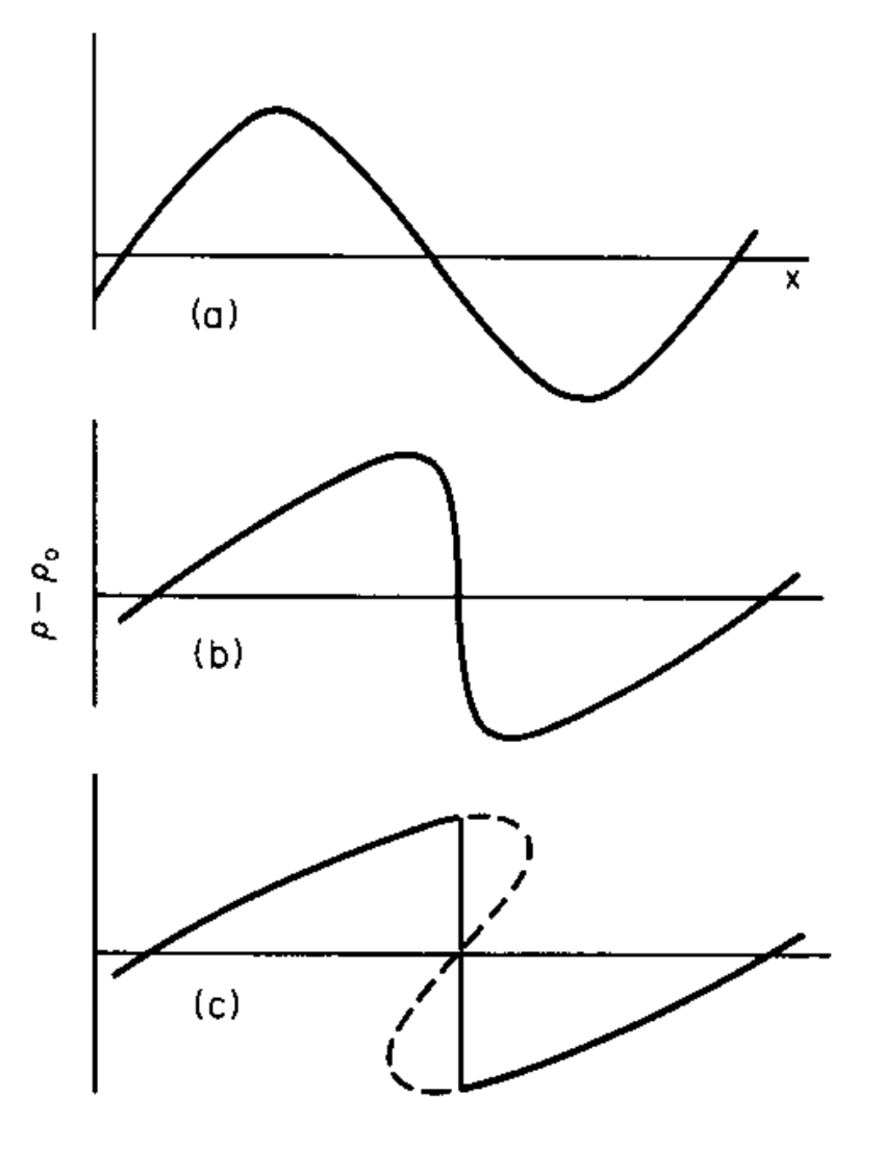
\includegraphics[width=0.5\textwidth]{figures/shocklandau.pdf}
\caption{}
\label{fig:landau}
\end{figure}

In fact, shock waves are a ubiquitous feature in astrophysical environments, reflecting the variety of processes that drive supersonic motion. 
%
Notable examples include:
\begin{itemize}
\item Fast stellar winds collide with the interstellar medium, forming bow shocks or termination shocks.  
\item Supernova blast waves plow into the surrounding medium.  
\item In gamma-ray bursts, colliding relativistic shells generate shocks within the ejecta.  
\item Matter falling onto compact objects like neutron stars or black holes forms accretion shocks.  
\item Shock waves develop as material accretes onto galaxy clusters' hydrostatic intracluster medium.  
\end{itemize}

Their presence in is a testament to the dynamic, high-energy processes shaping the universe.

\end{document}

\section{Interstellar Shock Waves}

\begin{figure}[!t]
\centering
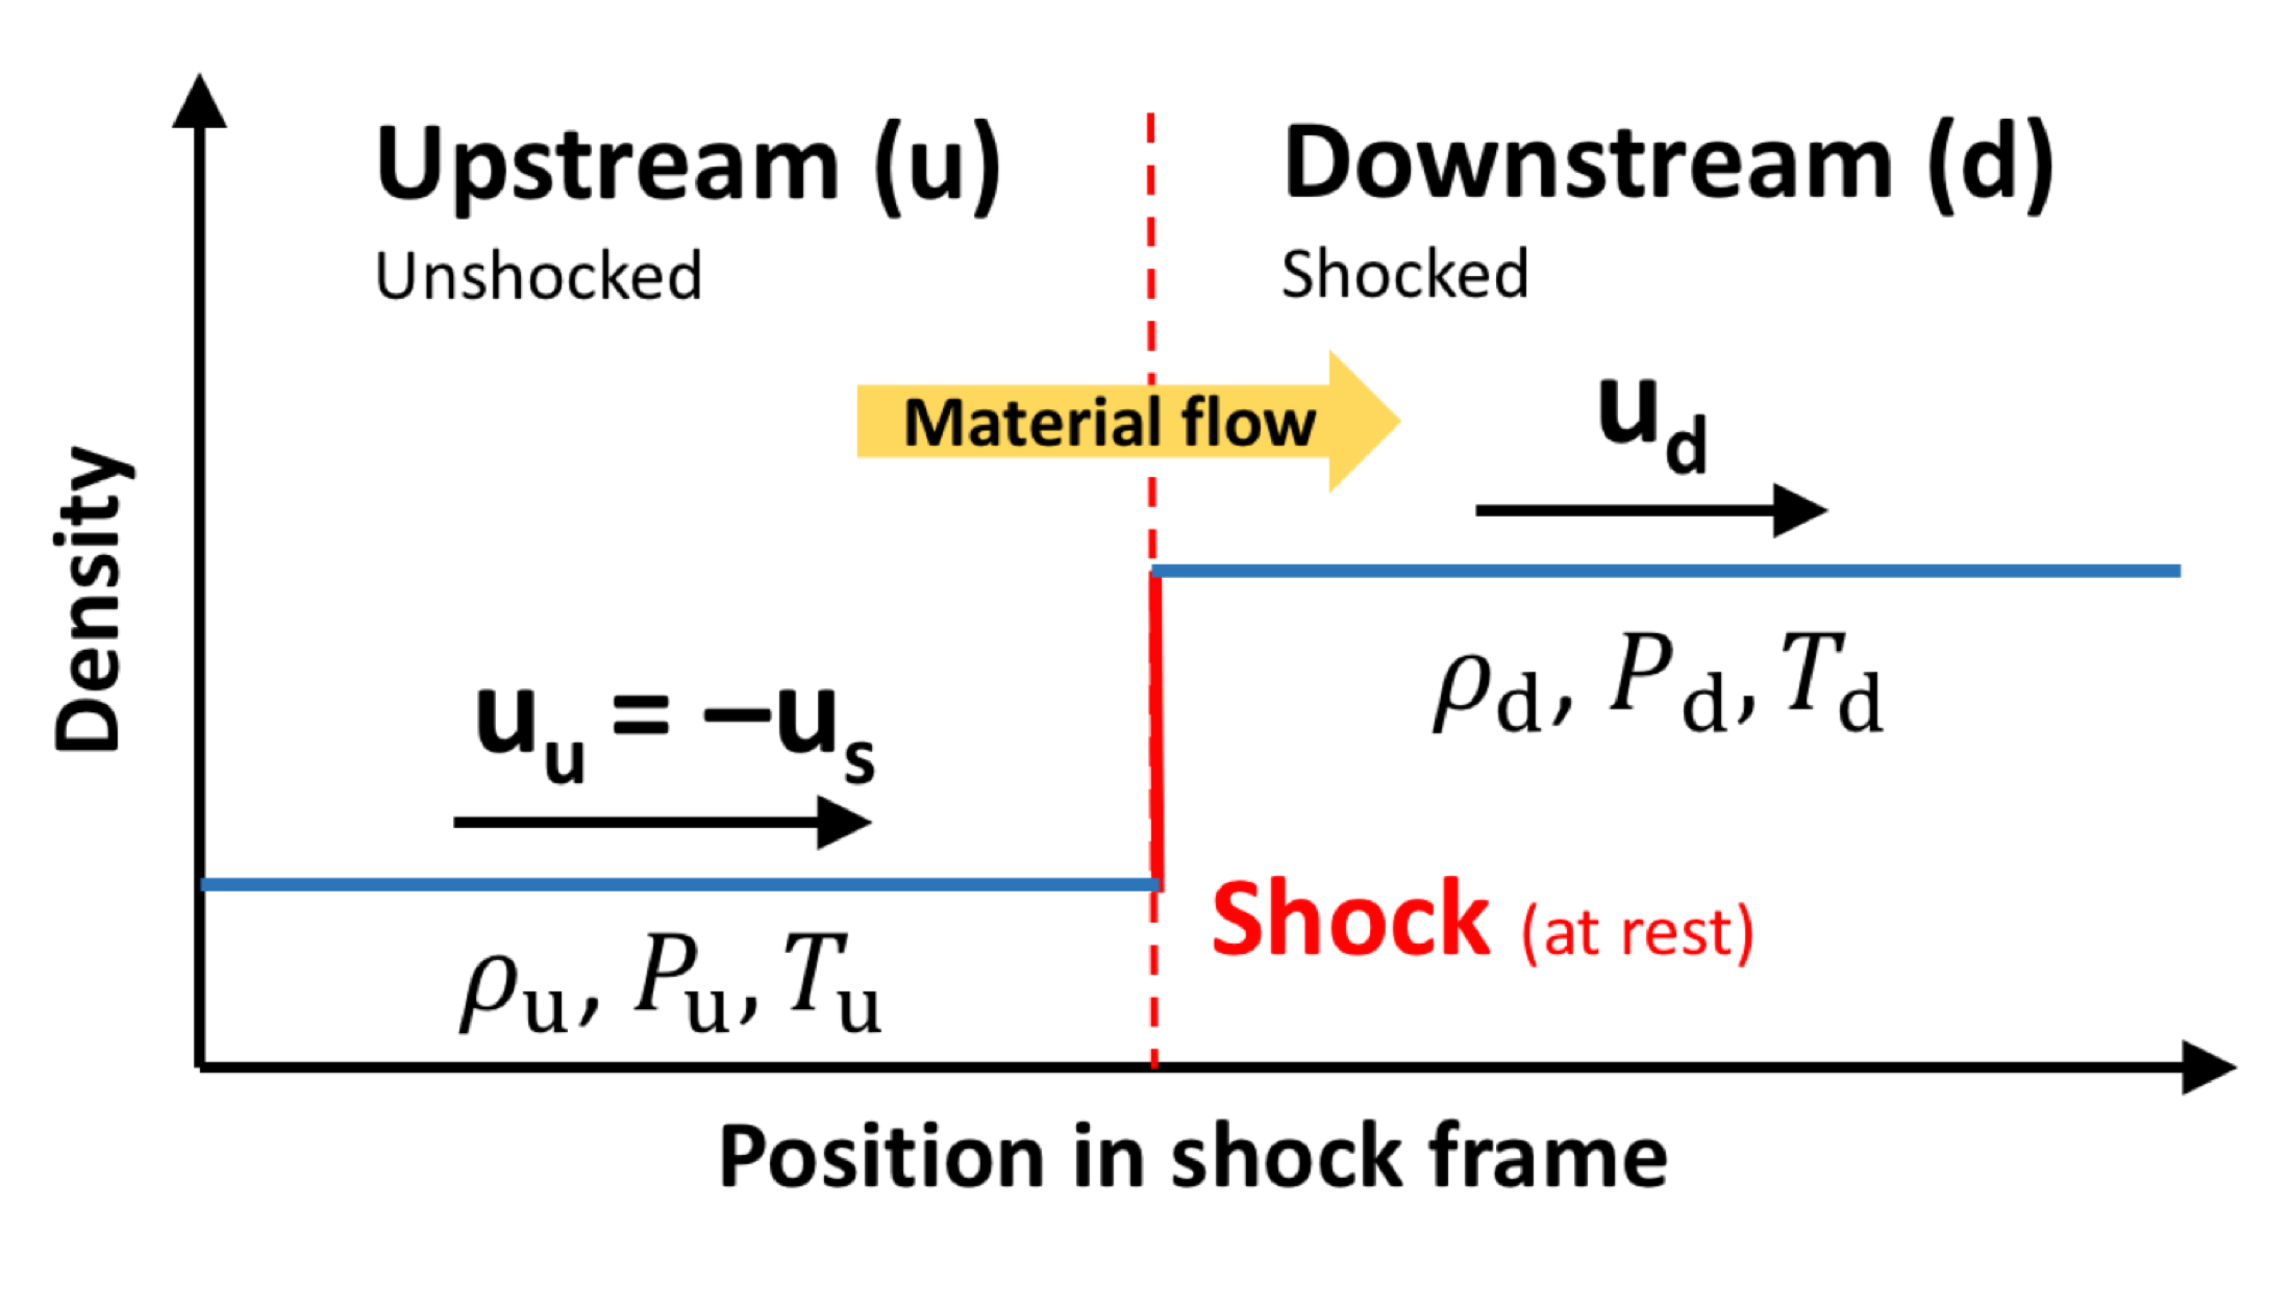
\includegraphics[width=0.5\textwidth]{figures/downupstream.pdf}
\caption{}
\end{figure}

Hydrodynamics often presents discontinuous solutions, meaning that there exist surfaces where physical quantities change abruptly. Mathematically, this is represented by differing values at the left and right limits of a point. However, physically, this discontinuity is not infinitely sharp as suggested in mathematical theory; rather, the change occurs over a region smaller than all other physical scales involved. 
%
A \emph{shock} is a specific type of discontinuity characterized by a surface that separates two fluid regions with differing properties. Importantly, this surface allows for the transfer of mass, momentum, and energy across it.

As seen beforehand, shocks are a natural consequence in the non-linear regime of fluid dynamics or magnetohydrodynamics (MHD).

Shocks are especially relevant in astrophysics; the gas post-shock emits significantly more than pre-shock gas, making these events more detectable.

Unlike terrestrial shocks, astrophysical shock waves are predominantly \textbf{collisionless}. 
%
In standard atmospheric conditions, where the number density of particles is approximately \( n \sim 10^{23} \, \text{cm}^{-3} \), and the cross-section for collisions\footnote{In the case of neutral particles, the hard sphere approximation holds true, where \( \sigma = \pi (r_A + r_B)^2 \) with \( r \) denoting the atomic radii of the colliding atoms.} around \( \sigma \sim 10^{-16}~\text{cm}^2 \), the mean free path \( \lambda \simeq 1 / (n \sigma) \) of a particle is \( \simeq 10^{-7}~\text{cm} \). 
%
In such conditions, \textbf{collisions} between particles are frequent, leading to the transformation of ordered kinetic energy into disordered (thermal) kinetic energy, characteristic of a collisional shock.

In contrast, astrophysical environments, where most particles are ionized, present a different scenario. The cross-sections for ionized particles are typically on the order of \( \sigma \sim \pi r_0^2 \sim 10^{-26}~\text{cm}^2 \) as $r_0 \sim$~fm is now the \textbf{nuclear} radius.
%
More importantly, these environments have much lower particle densities, about \( n \sim 1~\text{cm}^{-3} \). As a result, the mean free path in such settings is \( \gg \) Mpc! 
%
This means that the formation of the shock and its energy dissipation mechanisms do not primarily occur through particle collisions or Coulomb interactions. Instead, these processes are predominantly governed by interactions with the ambient magnetic field. The detailed microphysics of astrophysical shocks are complex and beyond the scope of this discussion.

Despite the microscale complexity at discontinuities (e.g., finite conductivity determining the size), conservation laws of mass, momentum, and energy remain applicable.

For non-relativistic shock waves, we can define the reference frame of the unshocked medium or \textbf{Galaxy frame}, where \( u^\prime_1 = 0 \),
the shock propagates into the unshocked medium at a speed \( u^\prime_s \), while the speed of shocked gas is \( u^\prime_2 (< u^\prime_s) \).

More convenient is to use a frame of reference  where the discontinuity surface is stationary, with \( u_s = 0 \). So the upstream medium approaches it at a speed \( u_1 = -u^\prime_s \), while the shocked fluid moves away from the shock front at a speed \( u_2 = u^\prime_s - u^\prime_2 \).
%
Consequently, the relative speed between the shocked and unshocked fluids is \( u_{\text{rel}} = u_1 - u_2 \).

In the following, it will be easier to refer our equations to the \textbf{shock front frame}, and we will categorize the physical quantities based on their position relative to the shock: those \textbf{upstream} of the shock are labeled as '1' and those \textbf{downstream} as '2'.\footnote{Use instead u and d.}

In the context of shock dynamics, we will focus on key thermodynamic quantities: density, pressure, temperature, and momentum across the two media (upstream and downstream of the shock). To analyze these, we first want to write conservation equations in the form \( \frac{dJ}{dz} = 0 \), where \( J \) represents the flux of a conserved quantity (be it mass, energy, or momentum).

Following this approach, it implies:
%
\begin{equation}
\int_{-\epsilon}^{\epsilon} \frac{dJ}{dx} = J_2 - J_1 = 0
\end{equation}

As common here, we introduce the notation \( [J]_{\text{sh}} = 0\) to denote the change in the flux across the shock expressed as \( J_2 - J_1 = 0 \). 

Let us summarize the key transport equations for a fluid, assuming that the only acting force density is the pressure gradient \( \nabla P \), and neglecting the effects of magnetic or gravitational fields.

First, the mass continuity equation is given by:
%
\begin{equation}
\frac{\partial \rho}{\partial t} + \nabla \cdot (\rho \mathbf{u}) = 0
\end{equation}
%
where \( \rho \) represents the fluid density, and \( \mathbf{u} \) is the fluid velocity.

Next, the conservation of momentum per unit volume is described by:
%
\begin{equation}
\rho \frac{\partial \mathbf{u}}{\partial t} + \rho (\mathbf{u} \cdot \nabla) \mathbf{u} = -\nabla P
\end{equation}

Finally, the conservation of energy per unit volume is expressed as:
%
\begin{equation}
\frac{\partial}{\partial t} \left( \frac{1}{2} \rho u^2 + \rho U \right) + \nabla \cdot \left[ \mathbf{u} \left( \frac{1}{2} \rho u^2 + \rho U + P \right) \right] = 0
\end{equation}
%
here \( \epsilon = \rho U \) denotes the internal energy per unit volume.

For our analysis, we focus on a one-dimensional (planar) shock in a stationary state (\( \partial_t \rightarrow 0 \)) and apply these conservation laws within the reference frame where the discontinuity is stationary.

Applying the mass continuity equation, we derive:
%
\begin{equation}\label{eq:mass}
\frac{\partial}{\partial z} (\rho u) = 0
\end{equation}

Next, from the momentum equation, and utilizing the mass continuity equation in Eq.~\ref{eq:mass}, we obtain:
%
\begin{equation}
\rho u \frac{\partial u}{\partial z} = -\frac{\partial P}{\partial z}  \, \rightarrow \, \frac{\partial}{\partial z} (P + \rho u^2) = 0 
\end{equation}

%Here, \( P_{\text{g}} \) represents the gas pressure.

Moving to the energy equation and again invoking the continuity equation, we find:
%
\begin{equation}
\frac{\partial}{\partial z} \left( \rho u \left[ \frac{1}{2} u^2 + U + \frac{P}{\rho} \right] \right) = 0 
\end{equation}

This can be expressed in terms of specific enthalpy \( w \) (see Appendix):
%
\begin{equation}
w = U + \frac{P}{\rho} = \frac{\gamma}{\gamma - 1}\frac{P}{\rho}
\end{equation}

Therefore, we arrive at the equation:
%
\begin{equation}
\frac{\partial}{\partial z} \left( \frac{1}{2} u^2 + \frac{\gamma}{\gamma - 1}\frac{P}{\rho} \right) = 0 
\end{equation}

Summarizing, assuming planar geometry, and in the frame of the shock, the conservation of fluxes of mass, momentum energy across the shock write
%
\begin{remark}
\begin{eqnarray}
\left[ \rho u \right]_{\rm sh} & = & 0 \label{eq:RH1} \\
\left[ \rho u^2 + P \right]_{\rm sh} & = & 0 \label{eq:RH2} \\
\left[ \frac{1}{2} u^2 +\frac{\gamma}{\gamma - 1} \frac{P}{\rho} \right]_{\rm sh} & = & 0 \label{eq:RH3}
\end{eqnarray}
\end{remark}

These conditions are known as the \textbf{Rankine-Hugoniot jump conditions}. They represent the dynamical equations for solutions that express conservation across the discontinuity of a shock, essentially establishing relationships between quantities on either side of the shock front.

We are dealing with three unknowns and have three corresponding equations. Apart from the trivial solution where all quantities remain constant, our aim is to derive the non-trivial solution.

To proceed, we remind the definition of sound speed:
%
\begin{equation}
c_{\text{s}} = \left( \frac{\partial P}{\partial \rho} \right)^{1/2} = \left(\frac{\gamma P}{\rho}\right)^{1/2}
\end{equation}

Here, we assume an ideal gas so the equation of state is \( P = K \rho^\gamma \), with \( \gamma \) being the ratio of specific heats. For a mono-atomic gas, in particular, \( \gamma = 5/3 \).

We then define the Mach number as the ratio of the shock speed to the sound speed in region \( i \), denoted as \( \mathcal{M}_i = v_i / c_{\text{s}} \). From this, it follows that:
%
\begin{equation}
\rho_i u_i^2 + P_i = \rho_i c_{\text{s}, i}^2 \left( \frac{u_i^2}{c_{\text{s},i}^2} \right) + P_i = (1 + \gamma \mathcal{M}_i^2) P_i
\end{equation}

If we fix the quantities in the upstream region,  $\rho_1$,  $u_1$ and $P_1$, hence solving the equations for the downstream using Eq.s~\ref{eq:RH1}-\ref{eq:RH3} will lead us to (see Appendix):
%
\begin{eqnarray}
\frac{\rho_2}{\rho_1} & = & \frac{u_1}{u_2}=\frac{(\gamma +1) \mathcal M_1^2}{(\gamma - 1) \mathcal M_1^2+2} \\
\frac{P_2}{P_1} & = & \frac{2\gamma \mathcal M_1^2}{\gamma +1}-\frac{\gamma -1}{\gamma +1} \\
\frac{T_2}{T_1} & = & \frac{\left[2\gamma \mathcal M_1^2 -(\gamma - 1) \right] \left[ (\gamma - 1) \mathcal M_1^2 + 2 \right]}{(\gamma + 1)^2 \mathcal M_1^2}
\end{eqnarray}

Under the assumption of strong shock conditions, characterized by \( \mathcal{M}_1 \gg 1 \), and considering a monoatomic gas with \( \gamma = 5/3 \), we can deduce the jump in density:
%
\begin{remark}
\begin{equation}
r = \frac{\rho_2}{\rho_1} = \frac{u_1}{u_2} = \frac{\gamma + 1}{\gamma - 1} = 4
\end{equation}
\end{remark}
%
here, \( r \) represents the compression factor, defined as \( \frac{\rho_2}{\rho_1} \). This factor is dependent on the adiabatic index \( \gamma \) and the Mach number of the shock. It's noteworthy that the compression factor cannot exceed 4.

For the pressure jump, we obtain:
%
\begin{equation}
\frac{P_2}{P_1} = \frac{2 \gamma}{\gamma + 1} \mathcal{M}_1^2 = \frac{5}{4} \mathcal{M}_1^2 
\end{equation}

From the frame of reference at the discontinuity, we observe an approaching gas with velocity \( u_1 \), which is altered to \( u_2 \approx \frac{1}{4}u_1 \) on the opposite side. Consequently, the plasma is decelerated and becomes denser.
%
However, energy conservation dictates that this energy must transform into \textbf{heat}. Examining the temperature ratio \( \frac{T_2}{T_1} \) under the same conditions, we find:
%
\begin{equation}
\frac{T_2}{T_1} = \frac{2 \gamma (\gamma - 1)}{(\gamma +1)^2} \mathcal{M}_1^2
\end{equation}

Therefore:
%
\begin{remark}
\begin{equation}
k_B T_2 = k_B T_1 \frac{2 \gamma (\gamma - 1)}{(\gamma +1)^2} \frac{u_1^2}{c_{\text{s},1}^2} = \frac{3}{16} m_p u_1^2
\end{equation}
\end{remark}

In this equation, we have utilized \( \rho_i = n_i m_p \), \( \mathcal{M}_i^2 = \frac{u_i^2}{c_{\text{s},i}^2} \), \( c_{\text{s},i}^2 = \frac{\gamma P_i}{\rho_i} \), and \( P_i = n_i k_B T_i \).

It's interesting to note that for typical astrophysical shocks, with \( u_1 \gtrsim 10^4 \) km/s, the temperature \( T_2 \) reaches approximately \( \sim 10^7 \) K.
%
This is what happens for example in a supernova explosion \( \mathcal M \sim 10^3 \) or in a GRB.  The plasma crosses shocks and heats up until it starts radiating in X-ray.

In summary, shocks convert \textbf{bulk kinetic energy of upstream medium to thermal (internal) energy downstream}.

\begin{remark}
The plasma behind the shock is
\begin{itemize}
\item Compressed \( \rho_2 = 4 \rho_1 \)
\item Slown down \( v_2 = \frac{1}{4} v_1 \)
\item Heated \( T_2 \ll T_1 \)
\end{itemize}
\end{remark}

The transformation of inflow kinetic energy into thermal energy in shock waves is accompanied by the generation of entropy. The key to this transformation is the collisions among particles within the shock wave. These collisions convert the ordered bulk kinetic energy, where particle velocities are aligned, into disordered internal kinetic energy, or heat.

However, as we have previously noted, the mean free path for collisions in astrophysical conditions can be macroscopically large. In such scenarios, energy exchange among particles is mediated by electromagnetic fields.
%
Therefore, the thickness of the shock is more characterized by the non-relativistic Larmor radius of a proton. This radius reflects the scale over which particles are deflected by the magnetic field present at the shock front.

Considering a typical proton velocity of \( \sim 10^4 \) km/s in a supernova explosion, and within a typical galactic magnetic field of \( 1 \mu \)G, the Larmor radius (\( r_{\text{B}} \)) is calculated as:
%
\begin{equation}
r_{\text{B}} = \frac{m_p v c}{e B} \simeq 10^{10}~\text{cm}
\end{equation}

When compared to typical lengths involved in supernova (SN) explosions, which are on the order of a parsec (see later), the shock thickness is several orders of magnitude smaller. Therefore, in the grand scale of such astrophysical phenomena, the approximation of an infinitely thin shock layer is justified.

Finally, we want to compute the post-shock Mach number \( M_2 \):
%
\begin{equation}
\mathcal M_2 = \frac{u_2}{c_{\rm s,2}} = \mathcal M_1 \frac{u_2}{u_1} \frac{c_1}{c_2} = \mathcal M_1 \frac{u_2}{u_1} \left( \frac{T_1}{T_2} \right)^{1/2}
\end{equation}
%
in the strong shock limit:
%
\begin{equation}
\mathcal M_2 = \mathcal M_1 \frac{\gamma - 1}{\gamma + 1} \left[ \frac{(\gamma + 1)^2}{2\gamma(\gamma - 1) \mathcal M_1^2} \right]^{1/2} = \left( \frac{\gamma - 1}{2\gamma} \right)^{1/2} \simeq 0.45 
\end{equation}
%
so a shock converts supersonic gas into subsonic gas.
%
In doing so, it increases the specific entropy of the gas by an amount~(see appendix):
%
\begin{equation}
s_2 - s_1 = c_{\rm P} \ln \left(\frac{T_2}{T_1}\right) - \frac{k}{m} \ln \left( \frac{P_2}{P_1} \right)
\end{equation}
%
In another terminology, a shock changes the entropy shifting gas to a higher adiabat.

Notice then that the non trivial solution makes sense only if the Mach number $M_1$ is larger than one. In the opposite case, we the variation of entropy would be in the sense to decrease it, which is not allowed by second principle of thermodynamics. 
%
In other words we would have invented a system to transform heat in ordered work! Shocks can only form in supersonic motion.

\subsection{Supernovae in the Milky Way}

Historical SNe: Kepler 1604, {\color{red}Tycho SNR 1572}, SN1006 SNR, Cas A 1680?

We distinguish between: 
%
\begin{itemize}
\item Core collapse supernovae (Type II, Ib/c,..)
\begin{itemize}
\item Progenitor: Massive star (\( \gtrsim 8~M_\odot \))
\item Energy source: gravitational collapse (\( \gtrsim 10^{53} \)~erg) 
\item Kinetic energy: \( \sim 10^{51} \)~erg
\item Ejecta mass \( >4~M_\odot \)  
\item Neutron star (or BH)
\end{itemize}
\item Thermonuclear supernovae (Type Ia)
\begin{itemize}
\item Progenitor: accreting CO white dwarf, or merging white dwarfs 
\item Energy source: nuclear fusion (C/O -> Fe-group)
\item Kinetic energy: \( 1.2 \times 10^{51} \) erg
\item Ejecta mass \( \sim 1.4~M_\odot \)
\item Total disruption of star
\end{itemize}
\end{itemize}
% !TEX root = ../lectures.tex
\section{Dynamical Evolution of Supernova Remnants}

\subsection{Supernovae in the Milky Way}

Historical SNe: Kepler 1604, {\color{red}Tycho SNR 1572}, SN1006 SNR, Cas A 1680?

We distinguish between: 
%
\begin{itemize}
\item Core collapse supernovae (Type II, Ib/c,..)
\begin{itemize}
\item Progenitor: Massive star (\( \gtrsim 8~M_\odot \))
\item Energy source: gravitational collapse (\( \gtrsim 10^{53} \)~erg) 
\item Kinetic energy: \( \sim 10^{51} \)~erg
\item Ejecta mass \( >4~M_\odot \)  
\item Neutron star (or BH)
\end{itemize}
\item Thermonuclear supernovae (Type Ia)
\begin{itemize}
\item Progenitor: accreting CO white dwarf, or merging white dwarfs 
\item Energy source: nuclear fusion (C/O -> Fe-group)
\item Kinetic energy: \( 1.2 \times 10^{51} \) erg
\item Ejecta mass \( \sim 1.4~M_\odot \)
\item Total disruption of star
\end{itemize}
\end{itemize}

Our goal is to model the explosion of a SN, which can be approximated as the instantaneous release of energy \( E \) at the origin (\( r = 0 \)) and at the initial moment (\( t = 0 \)). Assuming that the external medium is homogeneous and static, the motion of the resulting shock wave will be symmetrically radial.

In the initial phase of the explosion, the energy released is so immense that the effect of the density \( \rho_0 \) of the surrounding medium is negligible. 
%
This leads to the shock wave propagating at a constant, ballistic velocity, a stage known as the \emph{Free Expansion Phase}.

During this phase, an amount of matter \( M_{\rm ej} \) is ejected with velocity \( v_0 \) and kinetic energy \( E_{\rm SN} \). From this we can derive the constant velocity:
%
\[
E_{\rm SN} = \frac{1}{2} M_{\rm ej} v_0^2 \rightarrow v_0 = 10^4 \left( \frac{E_{\rm SN}}{10^{51}~\text{erg}} \right)^{1/2} \left( \frac{M_{\rm ej}}{M_\odot} \right)^{-1/2}~\text{km/s}
\]

This ejection velocity can be compared with the sound speed \( c_{\rm s} \) in the ISM:
%
\[
c_{\rm s} = \left( \gamma \frac{k T}{m_p} \right)^{1/2} \simeq 10 \left( \frac{T}{10^4~\text{K}} \right)^{1/2}~\text{km/s}
\]

For a monoatomic gas, \( \gamma = 5/3 \). Given these conditions, the Mach number (\( \mathcal M \)) is approximately \( 10^3 \), indicating that a \emph{strong} shock is indeed produced.

The evolution of the supernova remnant during this phase can be described simply by:
%
\begin{eqnarray*}
v_s & =  & v_0 \\
R_s & = & v_0 t 
\end{eqnarray*}

This phase is characterized by the shock wave expanding outward at a constant velocity, unimpeded by the surrounding medium.
 
The free expansion phase remains valid under the condition that the mass \( M_{\rm sw} \) swept up by the shock is negligible compared to the mass \( M_{\rm ej} \) of the ejecta:
%
\[
M_{\rm ej} \gg M_{\rm sw} \simeq \frac{4\pi}{3} R_s^3 \rho_0
\]

This condition ensures that the momentum of the ejecta is largely unaffected by the interstellar medium. However, as the shock wave expands, it accumulates more interstellar material, increasing \( M_{\rm sw} \).

Notice that shock waves generated by SN explosions may propagate through the ISM, or through the \emph{wind} of the progenitor star, where the density, \( \rho_0 \) is much smaller, hence the free expansion phase is longer.

When the swept-up mass becomes comparable to the ejecta's mass, the expansion of the remnant inevitably slows down. 
%
This transition occurs at a distance, denoted as \( R_{\rm ej} \), which can be approximated when \( M_{\rm ej} \simeq M_{\rm sw} \):
%
\[
R_{\rm ej} \simeq 2 \left( \frac{M_{\rm ej}}{M_\odot} \right)^{1/3} \left( \frac{n_0}{\text{cm}^{-3}} \right)^{-1/3}~\text{pc}
\]

Correspondingly, a characteristic time \( t_{\rm ej} \) can be determined for this phase:
%
\[
t_{\rm ej} \simeq \frac{R_{\rm ej}}{v_0} \simeq 2 \times 10^2 \left(\frac{M_{\rm ej}}{M_\odot}\right)^{5/6} \left(\frac{E_{\rm SN}}{10^{51}~\text{erg}}\right)^{-1/2} \left(\frac{n_0}{\text{cm}^{-3}}\right)^{-1/3}~\text{year}
\]

As the shock wave expands through the surrounding medium, it sweeps up and accumulates material, pushing it into a thin shell at the shock front. To estimate the thickness of this shell, we compare the total mass accumulated with the mass in a shell where the density is \( 4 \rho_0 \), reflecting the compression of the downstream material:
%
\[ \frac{4\pi}{3} R_{\rm s}^3 \rho_0 = 4 \pi R_{\rm s}^2 \Delta R (4 \rho_0) \]

From this, we derive the relative shell thickness: \[ \frac{\Delta R}{R_{\rm s}} = \frac{1}{12} \sim 10\% \] 

This calculation confirms the validity of the \emph{thin shell approximation}, indicating that the accumulated material forms a relatively narrow layer compared to the overall radius of the shock wave.

We can express the mass within this shell as:
%
\[
M = \cancel{M_{\rm ej}} + 4\pi \int_0^{R_{\rm s}} dR R^2 \rho_0 \simeq \frac{4\pi}{3} R^3_{\rm s} \rho_0
\]
%
where we assume that the mass of the ejecta is negligible compared to the mass of the swept-up material.

The expansion of the shock wave occurs adiabatically. In fact, for temperatures \( T \gtrsim 10^6 \)~K, the radiative cooling of the post-shocked gas is extremely inefficient as the cooling timescale is significantly longer than the expansion timescale of the shock wave. 

Given this adiabatic condition, we can apply the {\color{red}energy conservation equation}:
%
\[
E = E_k + E_{\rm th} 
= \frac{1}{2} M v_{\rm sh}^2 + \epsilon \frac{4\pi}{3} R^3_{\rm s} 
= \frac{1}{2} M v_{\rm sh}^2 + \frac{P_{\rm in}}{\gamma - 1} \frac{4\pi}{3} R^3_{\rm s} 
= \text{const}
\]

In the Sedov phase of SNR expansion, momentum conservation is governed by the equation:
%
\[
\frac{d}{dt} \left(M v_{\rm sh} \right) = 4\pi R^2_{\rm s} (P_{\rm in} - \cancel{P_{\rm out}})
\]


In the case of a strong shock, the external pressure \( P_{\rm out} \) is negligible compared to the over-pressurized internal gas, and thus it is omitted from the equation.

Seeking power law solutions, we propose a form for the shock radius:
%
\[ 
R_{\rm s} = A t^\alpha \rightarrow v_{\rm s} = \frac{dR_{\rm s}}{dt} = \frac{\alpha R_{\rm s}}{t} \propto t^{\alpha - 1}
\]

With this form, the momentum equation transforms into (using \(\gamma = \frac{5}{3} \)):
%
\[
\frac{\rho_0}{4} \frac{d}{dt} (R_s^3 v_s) = R_s^2 P_{\rm in} \rightarrow P_{\rm in} = \frac{(4\alpha - 1)}{4\alpha} \rho_0 v_s^2
\]

Here, we utilize the mass expression from a previous equation and the velocity relation downstream, \( v_{\rm sh} = \frac{3}{4} v_s \).

Consequently, the total energy of the system is given by:
%
\[
E = \frac{\pi}{8} \rho_0 A^5 \alpha (19 \alpha - 4) t^{5\alpha-2}
\]

Since the Sedov phase is characterized by constant total energy, the value of \( \alpha \) and \( A \) are determined as:
%
\[ 
\alpha = \frac{2}{5} \quad \text{and} \quad A = \left( \frac{50}{9\pi} \frac{E_{\rm SN}}{\rho_0} \right)^{1/5} 
\]

We conclude that during the Sedov phase, the energy distribution is such that one-third of the total energy is kinetic (\( E_k / E = 1/3 \)), while two-thirds is thermal (\( E_{\rm th} / E = 2/3 \)). 

%%% END CGPT

%We know \( M = \frac{4\pi}{3} \rho_0 R^3_s \) , \( \gamma = 5/3 \), \( v_{\rm sh} = 3/4 v_s \)
%{\color{red}shell speed - shock speed}

By substitution we find the evolution equation for radius and velocity
%
\[
R_{\rm s} \simeq 5~\left(\frac{E_{\rm SN}}{10^{51}~\text{erg}}\right)^{1/5} \left(\frac{n_0}{\text{cm}^{-3}}\right)^{-1/5} \left(\frac{t}{\text{kyr}}\right)^{2/5}~\text{pc}
\]
%
and
%
\[
v_{\rm s} \simeq 2 \times 10^3~\left(\frac{E_{\rm SN}}{10^{51}~\text{erg}}\right)^{1/5} \left(\frac{n_0}{\text{cm}^{-3}}\right)^{-1/5} \left(\frac{t}{\text{kyr}}\right)^{-3/5}~\text{km}~\text{s}^{-1}
\]

To determine the end of the Sedov phase we need to compute the cooling timescale, \( \tau_{\rm cool} \), and determine at which age the shell become radiative which corresponds to \( t_{\rm age} \sim \tau_{\rm cool} \)

The cooling time is given by the thermal energy divided the cooling rate
%
\[
\tau_{\rm c} \simeq \frac{\epsilon_{\rm th}}{n_i n_e \Lambda} \simeq \frac{3 \cancel{n} k_{\rm B} T}{n^{\cancel{2}} \Lambda} \simeq 10^6 \left( \frac{n_0}{\text{cm}^{-3}} \right)^{-1} \left( \frac{v_{\rm s}}{10^3~\text{km/s}} \right)^3~\text{yr}
\]
%
where we assumed full ionized gas \( n_i \sim n_e \) and for the cooling function we adopted a value derived from~\cite{}
%
\[
\Lambda \simeq 2 \times 10^{-19} T^{-1/2}~\text{erg}~\text{cm}^3~\text{s}^{-1}
\]

Using the cooling time just derived we find that the shell becomes radiative at an age:
%
\[
t_{\rm S} \simeq 2 \times 10^4 \left( \frac{E_{\rm SN}}{10^{51}~\text{erg}}\right)^{3/14} \left( \frac{n_0}{\text{cm}^{-3}} \right)^{-4/7}~\text{yr}
\]

\[
R_{\rm S} \simeq 20 \left( \frac{E_{\rm SN}}{10^{51}~\text{erg}} \right)^{1/14} \left( \frac{n_0}{\text{cm}^{-3}} \right)^{1/7}~\text{km}~\text{s}^{-1}
\]

%%% https://iopscience.iop.org/article/10.1086/305704/fulltext/36680.text.html
\newpage

\chapter{Particle Acceleration}
% !TEX root = ../lectures.tex
\section{How to Accelerate Cosmic Particles?}

Accelerating a particle means increasing its energy. In the vastness of the universe, most regions have temperatures ranging between \( 10^5 \, \text{K} \) and \( 10^8 \, \text{K} \). These correspond to particle energies of approximately \( 10 \, \text{eV} \) to \( 10 \, \text{keV} \).

At these temperatures, the universe predominantly exists in the \emph{plasma state}\footnote{Hydrogen's ionization energy is 13.6 eV.}, where protons and electrons are not bound into atoms but instead move independently. Plasma is the fundamental state of matter in stars, nebulae, and much of the interstellar medium.

However, particles in cosmic rays exhibit energies that far exceed this range: How do particles achieve such extreme energies?

The only known mechanism to increase the energy of a charged particle is through an \emph{electric field}, as electric fields exert forces that directly accelerate charged particles. Yet, this process faces a critical obstacle in astrophysical plasmas: the rapid motion of free electrons relative to protons in a plasma effectively short-circuits electric fields, preventing sustained acceleration\footnote{The only occurrence in which an electric field plays an important role in particle acceleration is the \emph{unipolar inductor}~\cite{}.}.
%   
On the other hand, while magnetic fields are ubiquitous in the universe, they only alter the direction of particle motion and cannot increase particle energy directly.

How can particles in a plasma --- where electric fields are neutralized and magnetic fields deflect rather than accelerate --- be energized to the levels observed in cosmic rays? The answer lies in \emph{magnetic induction}. Electric fields can be induced in a plasma when magnetic fields are dynamic --- that is, when they change over time or move relative to the plasma. This principle, encapsulated in \emph{Faraday's law of induction}, forms the foundation of many astrophysical particle acceleration mechanisms.

According to Faraday's law, a time-varying magnetic field generates an electric field:
\[
\vb\nabla \times \vec{\mathcal E} = -\frac{1}{c} \frac{\partial \vec{\mathcal B}}{\partial t}.
\]

Dimensionally, this relationship implies:
\begin{equation}
\frac{\mathcal E}{L} \sim \frac{1}{c} \frac{\mathcal B}{T} \, \longrightarrow \, \mathcal E \sim \frac{u}{c} \mathcal B~,
\end{equation}
where \( L \) is the characteristic size of the system, \( T \) is the timescale of magnetic field variation, and \( u \) is the velocity associated with the system.

For a particle of charge \( q \), this electric field translates to a maximum energy gain:
\begin{equation}\label{eq:Hillas1}
E_{\rm max} \sim q \, \mathcal E \, L \sim \frac{q}{c} \, L \, \mathcal B \, u.
\end{equation}
or \TODO{numerically}
\[
E_{\rm max} \sim 3 \times 10^{12} Z \left( \frac{B}{\mu\text{G}} \right) \left( \frac{u}{10^3~\text{km/s}} \right) \left( \frac{L}{\text{pc}} \right)~\text{eV}
\]

This shows that achieving significant acceleration requires:
%
\begin{itemize}
\item Large system sizes (\( L \)),
\item Strong magnetic fields (\( \mathcal B \)),
\item Fast-moving magnetic structures (\( u \)).
\end{itemize}

Assuming \( u \sim c \) (the most optimistic case), the confinement condition becomes:
\begin{equation}
r_{\rm L} \lesssim L,
\end{equation}
where \( r_{\rm L} = \frac{E}{q \mathcal B} \) is the particle's Larmor radius. 

This relation shows that to accelerate a particle effectively, the particle must remain confined within the accelerator. 
%
This condition leads to the \emph{Hillas criterion}~\cite{Hillas1984}, which sets a key limit on the maximum particle energy. 

The total magnetic energy, \( W_B \), in the acceleration system is given by the product of the magnetic energy density, \( \frac{\mathcal{B}^2}{8\pi} \), and the volume of the accelerator, \( \frac{4\pi}{3} \, L^3 \):  
\begin{equation}
W_B \sim \frac{\mathcal{B}^2 L^3}{6} \sim \frac{E_{\rm max}^2 L}{6 q^2},
\end{equation}
where we have made use of the Hillas criterion in equation~\ref{eq:Hillas1} to relate the magnetic field strength \( \mathcal{B} \), system size \( L \), and maximum particle energy \( E_{\rm max} \).  

\TODO{Numerically}, this gives:
\begin{equation}
W_B \sim 5 \times 10^{52} Z^{-1} \left( \frac{E_{\rm max}}{10^{20}~\text{eV}} \right)^2 \left( \frac{L}{\text{pc}} \right)~\text{erg}~.
\end{equation}

This total magnetic energy, \( W_B \), cannot exceed the total energy injected by the source. In other words, the accelerator’s magnetic energy must be derived from the energy supplied by the astrophysical system driving it.

For reference, a single supernova releases approximately \( 10^{51} \, \text{erg} \) as kinetic energy. This comparison highlights that to accelerate particles to extreme energies, we require \emph{extremely energetic astrophysical accelerators}.

Notice that an implicit assumption in deriving the Hillas criterion is that energy losses are negligible. In reality, however, this is not always the case, as particles can lose energy through radiation, collisions, or other interactions, oftentimes imposing stricter limits on the maximum achievable energy.

Moreover, we must note that the Hillas condition is a necessary but not sufficient condition to estimate whether or not a given energy can be achieve in a given type of source. In most case as the maximum energy estimated with this criterion is overoptimistic. 

In conclusion, identifying a good candidate for particle acceleration requires a system that satisfies the following conditions:  
\begin{itemize}
\item \emph{Large energetics}: The system must have a substantial energy reservoir to draw from --- be it kinetic energy (e.g., in supernova remnants), rotational energy (e.g., in pulsars), or gravitational potential energy (e.g., in accretion disks).
\item \emph{Sufficient confinement time}: Particles need to remain within the accelerator long enough to achieve significant energy gains.
\item \emph{Minimal energy losses}: Effective acceleration requires that energy losses (e.g., due to radiation or collisions) remain negligible during the acceleration process.
\item \emph{An efficient energy transfer mechanism}: There must be a way to transfer energy from macroscopic astrophysical phenomena into the microscopic acceleration of particles.
\end{itemize}

While several astrophysical systems meet the first three conditions --- possessing sufficient energy, scale, and lifetime to accelerate particles --- the mechanism of energy transfer remains a more complex problem. This challenge was first addressed by Enrico Fermi in 1949~\cite{}, laying the foundation for our understanding of particle acceleration in astrophysical contexts.

% !TEX root = ../lectures.tex
\section{Generalities of Stochastic Acceleration}

Stochastic acceleration, a cornerstone of high-energy astroparticle physics, describes the random and iterative energy gains experienced by particles within astrophysical accelerators. Let us explore the underlying principles in a structured manner.

In a stochastic acceleration process:
%
\begin{itemize}
\item Particles gain energy in \emph{cyclic encounters}, with each cycle requiring a characteristic time \( \tau \). 
\item During each cycle, there is a probability \( P_{\text{esc}} \) that a particle escapes the acceleration region, and a probability \( 1 - P_{\text{esc}} \) that it remains for further acceleration. 
\item The fractional energy gain per cycle is denoted by \( \xi \), implying that after one cycle, a particle with initial energy \( E_n \) becomes \( E_{n+1} = (1 + \xi) E_n \)~.
\end{itemize}

Over \( n \) cycles, a particle's energy evolves geometrically, leading to:
\begin{equation}
E_n = E_0 (1 + \xi)^n~,
\end{equation}
where \( E_0 \) is the initial energy. 
%
Consequently, the number of cycles required to reach a final energy \( E_n \) from \( E_0 \) is:
\begin{equation}
n = \frac{\ln \left( E_n/E_0 \right)}{\ln (1 + \xi)}~.
\end{equation}

Therefore, in this model, attaining significantly higher energies demands a \emph{larger number of acceleration cycles}.

Now consider the cumulative probability of a particle remaining in the acceleration region after \( n \) cycles:
\begin{equation}
P_{\text{survive}} = (1 - P_{\text{esc}})^n.
\end{equation}

The fraction of particles that reach energies exceeding a threshold \( E \) can be determined by summing the probabilities for particles that survive \( m \geq n \) cycles. Using the geometric series with ratio \( x = (1 - P_{\text{esc}}) \), we obtain:
\begin{equation}
f(>E) \propto \sum_{m=n}^\infty (1 - P_{\text{esc}})^m = \frac{(1-P_{\text{esc}})^n}{P_{\text{esc}}}~.
\end{equation}
Substituting for \( n \) using the energy relation:
\begin{equation}
f(>E) \propto \frac{(1-P_{\text{esc}})^{\frac{\ln \left( E/E_0 \right)}{\ln (1 + \xi)}}}{P_{\text{esc}}}~.
\end{equation}

Utilizing the logarithmic identity \( a^{\ln b} = b^{\ln a} \), this expression simplifies to a power-law distribution:
\begin{equation}
f(>E) \propto \frac{1}{P_{\text{esc}}} \left( \frac{E}{E_0} \right)^{\gamma}, \quad \text{where} \quad \gamma = \frac{\ln (1-P_{\text{esc}})}{\ln (1+\xi)}~.
\end{equation}

The parameter \( \gamma \) governs the spectral slope and can be approximated under the assumptions \( \xi \ll 1 \) and \( P_{\text{esc}} \ll 1 \):
\begin{remark}
\begin{equation}\label{eq:gammapescxi}
\gamma \simeq -\frac{P_{\text{esc}}}{\xi}.
\end{equation}
\end{remark}

Despite its simplicity, this framework highlights a universal feature of stochastic acceleration: it naturally produces a \emph{power-law energy distribution}, which is ubiquitous in astrophysical observations.  

The maximum energy achievable by this stochastic process is constrained by two primary factors:
\begin{itemize}
\item \emph{Finite Lifetime of the Accelerator}: The total time available for acceleration, \( T \), limits the number of cycles \( n \), with \( n_{\text{max}} \sim T / \tau \),
\item \emph{Energy-Dependent Escape Probability}: In realistic scenarios, the escape probability \( P_{\text{esc}} \) often increases with energy due to competing processes such as energy losses or dynamic changes in the accelerator. These factors eventually counteract the energy gains, capping the achievable energy.
\end{itemize}

Stochastic acceleration serves as a fundamental model for understanding cosmic particle spectra. Future sections will explore specific implementations, including Fermi second-order acceleration.
% !TEX root = ../lectures.tex
\section{Second-Order Fermi Mechanism}

{\color{red}Aggiungi plot.}

In 1949, Fermi proposed a physical system where this mechanism for particle acceleration can take place. In particular, he postulated the existence of an inhomogeneous interstellar medium, hence the presence of \emph{magnetic clouds} moving in random directions relative to the Galactic frame. These clouds, carrying magnetic fields, can reflect incoming charged particles.

The fundamental principle of the second-order Fermi mechanism is straightforward: \emph{particles gain energy when they encounter a magnetic cloud moving towards them and lose energy in encounters with clouds moving away}\footnote{This behavior mirrors a general property of elastic collisions in mechanics (see appendix~\ref{sec:app_collisions} for details on Newtonian collisions).}. Due to the greater frequency of head-on encounters compared to tail-on ones, there is an overall \emph{increase} in energy.

To quantify the energy change during a single interaction, we employ a double reference frame transformation: quantities measured in the magnetic cloud rest frame are denoted by primes, while those in the Galactic frame remain unprimed.

A particle with initial energy \( E_{\rm i} \) and momentum \( p_{\rm i} \) in the Galactic frame encounters a magnetic cloud moving along the \( x \)-axis with a velocity factor \( \beta = V / c \). We transform to the cloud rest frame, where the particle energy is given by\footnote{For simplicity, we have assumed the particle is relativistic, where \( p \simeq E \) (using units where \( c = 1 \))}:
\begin{equation}
E_i^\prime = \gamma (E_i - \beta p_{i,x}) = \gamma E_i \left( 1 - \beta \frac{p_{i,x}}{E_i} \right) = \gamma E_i \left( 1 - \beta \mu_i \right)
\end{equation}
where \( p_{i,x} \) is the component of the particle momentum along the cloud motion direction, and \( \mu_i = p_{i,x} / p_i = \cos\theta_i \) is the cosine of the angle between the particle velocity and the cloud velocity in the Galactic frame.

%- \( -1 \leq \mu_{\rm in} \leq 1 \), corresponding to all possible directions of particle motion relative to the cloud.

Upon reflection by the cloud, the particle energy, as observed externally, becomes:
\begin{equation}
E_f  = \gamma E_f^\prime \left(1+ \beta \mu^\prime_f \right) 
\end{equation}
where \( \mu^\prime_f \) is the cosine of the angle \emph{after} reflection in the cloud frame. Clearly, if $\beta$ is the cloud velocity in the Galactic frame, $-\beta$ is the Galactic frame velocity with respect to the cloud.

Since magnetic fields do not perform work on the particles, the particle undergoes only elastic scattering within the cloud. This means its energy upon exiting the cloud remains unchanged in the cloud's frame of reference, so that \( E^\prime_f = E^\prime_i \), and thus
%
\begin{equation}
E_f = \gamma^2 E_i \left(1 - \beta \mu_i + \beta \mu^\prime_f - \beta^2 \mu_i \mu^\prime_f \right)
\end{equation}

The relative change in energy after one encounter is:
%
\begin{equation}
\frac{\Delta E}{E} = \frac{E_f - E_i}{E_i} =
\gamma^2  \left(1 - \beta \mu_i + \beta \mu^\prime_f - \beta^2 \mu_i \mu^\prime_f \right) - 1
%= \frac{ \beta^2 - \beta \mu_{\rm in} + \beta \mu^\prime_{\rm out} - \beta^2 \mu_{\rm in} \mu^\prime_{\rm out}}{1-\beta^2} 
%simeq 2\beta^2 + 2\beta \mu
\end{equation}

This result shows that the energy gain is proportional to the initial energy, meaning \( \Delta E/E \) is independent of \( E \).

It is crucial to recognize that both energy gain and loss are possible in this mechanism. This variability arises because the movements of both particles and magnetic clouds (consequently, the angles of interaction \( \mu_i \) and \( \mu_f \)) are random. 
%
However, not all configurations are equally probable.

Given that a particle undergoes multiple scatterings off magnetic irregularities within the cloud, its exit direction becomes randomized, with an average \( \langle \mu^\prime_f \rangle = 0 \). 
%
Initially, we can average over the exit angle to get:
%
\begin{equation}
\left\langle \frac{\Delta E}{E} \right\rangle_{\mu^\prime} = 
\gamma^2 \left( 1 - \beta \mu_i \right) - 1
\end{equation}

{\color{red}Next, we must consider averaging over all possible initial angles. Since the frequency of particle-cloud collisions depends on their relative velocity, the probability distribution for the incoming angle is:
\begin{equation}
P(\mu) \propto v_{\rm{rel}} \propto 1 - \beta \mu_i  
\end{equation}}

Normalizing this probability over \( \mu_i \in [-1,1] \), we get:
\begin{equation}
P(\mu) = \frac{1 - \beta \mu_i}{2}
\end{equation}

Notice that \( \int_{\mu < 0} d\mu P(\mu) = 1 + \beta / 2 \) is larger than \( \int_{\mu > 0} d\mu P(\mu) = 1 - \beta/2 \), implying that \emph{head-on collisions} are more frequent compared to \emph{tail-on collisions}, which is the essence of Fermi's acceleration mechanism.

Consequently, the average change in energy is given by:
%
\begin{remark}
\begin{equation}
\left\langle \frac{\Delta E}{E} \right\rangle_{\mu\mu'} 
= \int_{-1}^{+1} d\mu \, P(\mu) \left[ \gamma^2 \left( 1 - \beta \mu \right) - 1 \right] \simeq \frac{4}{3} \beta^2
\end{equation}
\end{remark}

This confirms that Fermi's mechanism effectively accelerates charged particles: while individual interactions may result in energy gains or losses, the \emph{average energy change is positive}. However, the average energy gain is proportional to \( \beta^2 \), highlighting the fundamentally \emph{stochastic nature} of the process. 

For the second-order Fermi mechanism to account for the high-energy particles observed in cosmic rays, it must accelerate particles efficiently. Let us assess its viability within the ISM, where the typical cloud velocity is of the order of the Alfvén speed, \( v_A \sim 10 \, \text{km/s} \). In terms of \( \beta = v / c \), this translates to \( \beta \sim 10^{-4} \). 

The fractional energy change per encounter is therefore:
\[
\frac{\Delta E}{E} \sim \frac{4}{3} \beta^2 \sim 10^{-8},
\]
indicating a highly inefficient energy gain mechanism. 

To further quantify this inefficiency, we define the \emph{acceleration time}, \( \tau_{\rm acc} \), as the characteristic timescale for a particle to significantly increase its energy:
\[
\tau_{\rm acc} = \left( \frac{1}{E} \frac{dE}{dt} \right)^{-1}.
\]

Assuming the average distance between magnetic clouds is \( L \), and neglecting the magnetic field in the space between clouds (providing a lower limit), the average time between two encounters is:
\[
\tau_{\rm c} = \frac{L}{c}.
\]

The rate of energy gain is then:
\[
\frac{dE}{dt} \simeq \frac{\Delta E}{\tau_{\rm c}} = \frac{4}{3} \frac{\beta^2 c E}{L}.
\]

From this, the acceleration time can be expressed as:
\[
\tau_{\rm acc} = \frac{3}{4} \frac{L}{c \beta^2}.
\]

Using typical ISM values, \( \beta \sim 10^{-4} \) and \( L \sim 1 \, \text{pc} \), we find:
\[
\tau_{\rm acc} \gtrsim \text{Gyr}~,
\]
just for the particle to \emph{double its energy}. This timescale is vastly longer than the lifetimes of most astrophysical accelerators and is far too slow to explain the high energies observed in Galactic cosmic rays. In fact, particles in the ISM are subject to various energy loss mechanisms, such as ionization losses, that occur on timescales much shorter than \( \tau_{\rm acc} \), further diminishing the effectiveness of the second-order Fermi mechanism.

Another issue lies in the resulting energy spectrum. From previous discussions (see equation~\ref{Eq:slopegeneralized}), the spectrum slope depends on the ratio of the acceleration timescale \( \tau_{\rm acc} \) to the escape timescale \( \tau_{\rm esc} \). This ratio is highly variable across different regions of the Galaxy, depending on the density and velocity of magnetic clouds. As a result, the energy spectrum varies significantly between regions, thereby, when summed over the Galaxy, the contributions from different regions are unlikely to produce a coherent, universal power-law spectrum as observed for Galactic cosmic rays.

These limitations point to significant drawbacks of the second-order Fermi mechanism.
%
In contrast, \emph{diffusive shock acceleration} (discussed in the next section) circumvent these challenges. Shock fronts provide more efficient energy gain and yield spectra with consistent power-law behavior, making them far better candidates for explaining the acceleration of Galactic cosmic rays.

While it is unlikely to account for the bulk of cosmic-ray acceleration, however, the second-order Fermi mechanism may still play a role in cosmic-ray physics as in certain models of Galactic transport, interactions with turbulent magnetic fields driven by second-order Fermi-like processes can slightly \emph{re-energize} the spectrum of already-accelerated cosmic rays while they propagate through the Galaxy.

\subsection{Second-order Fermi re-acceleration}

{\color{red}To be done}

\subsection{Where do the cosmic ray get their energy?}

{\color{red}To be done}

%Note that in this scheme the magnetic field's primary role is to alter the direction of particle motion, but the magnetic field itself does not provide the energy to increase the particle energy. Instead, the energy is supplied by an induced electric field~{\color{red}approfondisci}.

%Furthermore, the energy gain does not depend on \( B \), the magnetic field strength. While the magnetic field mediates particle reflection, it does not directly appear in the Lorentz transformations.\todo{Approfondisci}

%As mentioned above, another possible way of working out the acceleration the to calculate the electric field seen in the Galactic frame by Lorentz transformation of the pure B field seen in the cloud frame. Since the two approaches must be equivalent the acceleration and the energy gain of the particle must also be independent of the cloud magnetic field in this case. This result is however far less intuitive with this approach.

%\begin{mdframed}
%\subsection*{Re-acceleration in the Fokker-Planck approach}
%
%Widely used for description of stochastic processes.
%%
%Let's define the probability that particle with momentum $\vb p$ at time $t$ changes momentum by $\Delta \vb p$ in time $\Delta t$.
%
%The phase space distribution function is $f(\vb x, \vb p, t)$ probability to find particle in phase space volume element d3xd3p.
%
%Using this defition
%%
%\begin{equation}
%f(\vb p, t+\Delta t) = 
%\int d^3(\Delta \vb p) \, f(\vb p - \Delta \vb p, t) P(\vb p - \Delta \vb p, \Delta \vb p)  
%\end{equation}
%
%Taylor expansion gives (to 2nd order in small $\Delta p$):
%%
%\begin{equation}
%f(\vb p, t) + \frac{\partial f}{\partial t} \Delta t \simeq \int d^3(\Delta \vb p) \, \left[ f P - \frac{\partial (fP)}{\partial p_i} \Delta p_i + \frac{1}{2} \frac{\partial^2 (fP)}{\partial p_i \partial p_j} \Delta p_i \Delta p_j + \dots \right]
%\end{equation}
%
%We impose now the normalization condition for the probability
%%
%\begin{equation}
%\int P(\vb p, \Delta \vb p) d^3 (\Delta p) = 1
%\end{equation}
%%
%and we define the Fokker-Planck coefficients as
%%
%\begin{eqnarray}
%\langle \Delta p_i \rangle & = & \int d^3 (\Delta p) P(\vb p, \Delta \vb p) \Delta p_i \\
%\langle \Delta p_i p_j \rangle&  = & \int d^3 (\Delta p) P(\vb p, \Delta \vb p) \Delta p_i \Delta p_j 
%\end{eqnarray}
%%
%which leads to
%%
%\begin{equation}
%\frac{\partial f}{\partial t} = 
%- \frac{\partial}{\partial p_i} \left( \frac{\langle \Delta p_i \rangle}{\Delta t} f \right) 
%+ \frac{1}{2} \frac{\partial^2}{\partial p_i \partial p_j} \left( \frac{\langle \Delta p_i \Delta p_j \rangle}{\Delta t} f \right)
%\end{equation}
%%
%with 1st term (rhs) describing systematic energy gain/losses, and 2nd diffu- sion part/dispersion/broadening.
%
%If scattering process is reversible in the sense that:
%%
%\begin{equation}
%P(\vb p, \Delta \vb p) = P(\vb p - \Delta \vb p, \Delta \vb p)
%\end{equation}
%
%\dots
%
%Fokker-Planck eq. then reduces to a diffusion equation in momentum space:
%%
%\begin{remark}
%\begin{equation}
%\frac{\partial f}{\partial t} = \frac{\partial}{\partial p_i} \left( D_{ij} \frac{\partial f}{\partial p_j} \right)
%\end{equation}
%\end{remark}
%%
%where $D_{ij}$ are the components of the diffusion tensor.
%\end{mdframed}

% !TEX root = ../lectures.tex
\section{First-Order Fermi Mechanism or Diffusive Shock Acceleration}

The mechanism often associated with Fermi is, in fact, the result of the work by several authors, as Krymsky, Bell, Blandford, and Ostriker in the late 1970s~\cite{addref}. 
%
%Krymsky, G. F. Dokl. Akad. Nauk SSSR 243, 1306 (1977). 13. 
%Bell, A. R. M.N.R.A.S. 182, 147 (1978).
%Axford, W. I., Leer, E., and Skadron, G. Proc. 15th ICRC (Plovdiv) XI, 132 (1977). 15. 
%Blandford, R. D. & Ostriker, J. P. Astrophys. J. Lett. 221, L29 (1978).
%
They discovered that \emph{astrophysical shocks} could act as extremely efficient accelerators for cosmic particles, a process now known as \emph{diffusive shock acceleration (DSA)}.

Current observations confirm that particles are indeed accelerated at these shocks, evidenced by the radiation emitted from such regions, typically interpreted as the energy losses of fresh accelerated electrons~\cite{ref}. 

We know at this point that \TODO{(see section)}, in the vicinity of the discontinuity, the upstream region is characterized by fast-moving, cold plasma, whereas the downstream region contains slower, hotter plasma. 
%
The typical shock wave's velocity in the ISM is approximately \( \sim 10^3-10^4 \) km/s, which corresponds to a Mach number of about \( 10^2-10^3 \), placing us firmly in the \emph{strong} shock regime.

The key concept here revolves around how particles perceive the plasma in the context of a shock front. 

From a particle's perspective, the plasma appears to approach at about the shock velocity from both the upstream (\( u \)) and downstream (\( d \)) sides. 
%
Consider a group of particles with energy \( E \) initially located on the \emph{upstream} side of the shock. These particles undergo diffusion through collisions with magnetic turbulence present in the plasma, which tends to isotropize their angular distribution in the frame where the upstream plasma is at rest.
%
Upon crossing the shock to the \emph{downstream} side, these particles encounter magnetic turbulence associated with the downstream plasma. This plasma is moving towards the particles at a velocity \( \sim \frac{3}{4} u_{\rm shock} \) in the same reference frame. If collisions with the downstream plasma further isotropize the particles, then from the particles' viewpoint, they effectively experience a collision with a \emph{cloud} moving towards them (head-on). 
%
Some of these particles will eventually diffuse back to the upstream side of the shock. Upon their return, they perceive the upstream plasma as moving towards them, on average. In the shock frame, the unshocked plasma advances towards the downstream at a speed of \( |u_u - u_d| \sim u_{\rm shock} \), resulting again in a \emph{head-on} cloud collision.
%
There are \emph{never} crossings in which the particles lose energy, and the increment in energy is the same going in both directions. At such, the continual diffusion of particles back and forth across the shock front can significantly accelerate the particles. 

As in both upstream and downstream scenarios, the particles experience head-on collisions, this mechanism will result in a \emph{first-order} Fermi acceleration.

%Therefore, numerous cycles of crossing the shock can significantly accelerate the particles. 
%Scattering ensures that once the particles enter in the upstream or downstream regions there their velocities become isotropically distributed.
%There are never crossings in which the particles lose energy, and the increment in energy is the same going in both directions.

\begin{figure}[t]
\centering
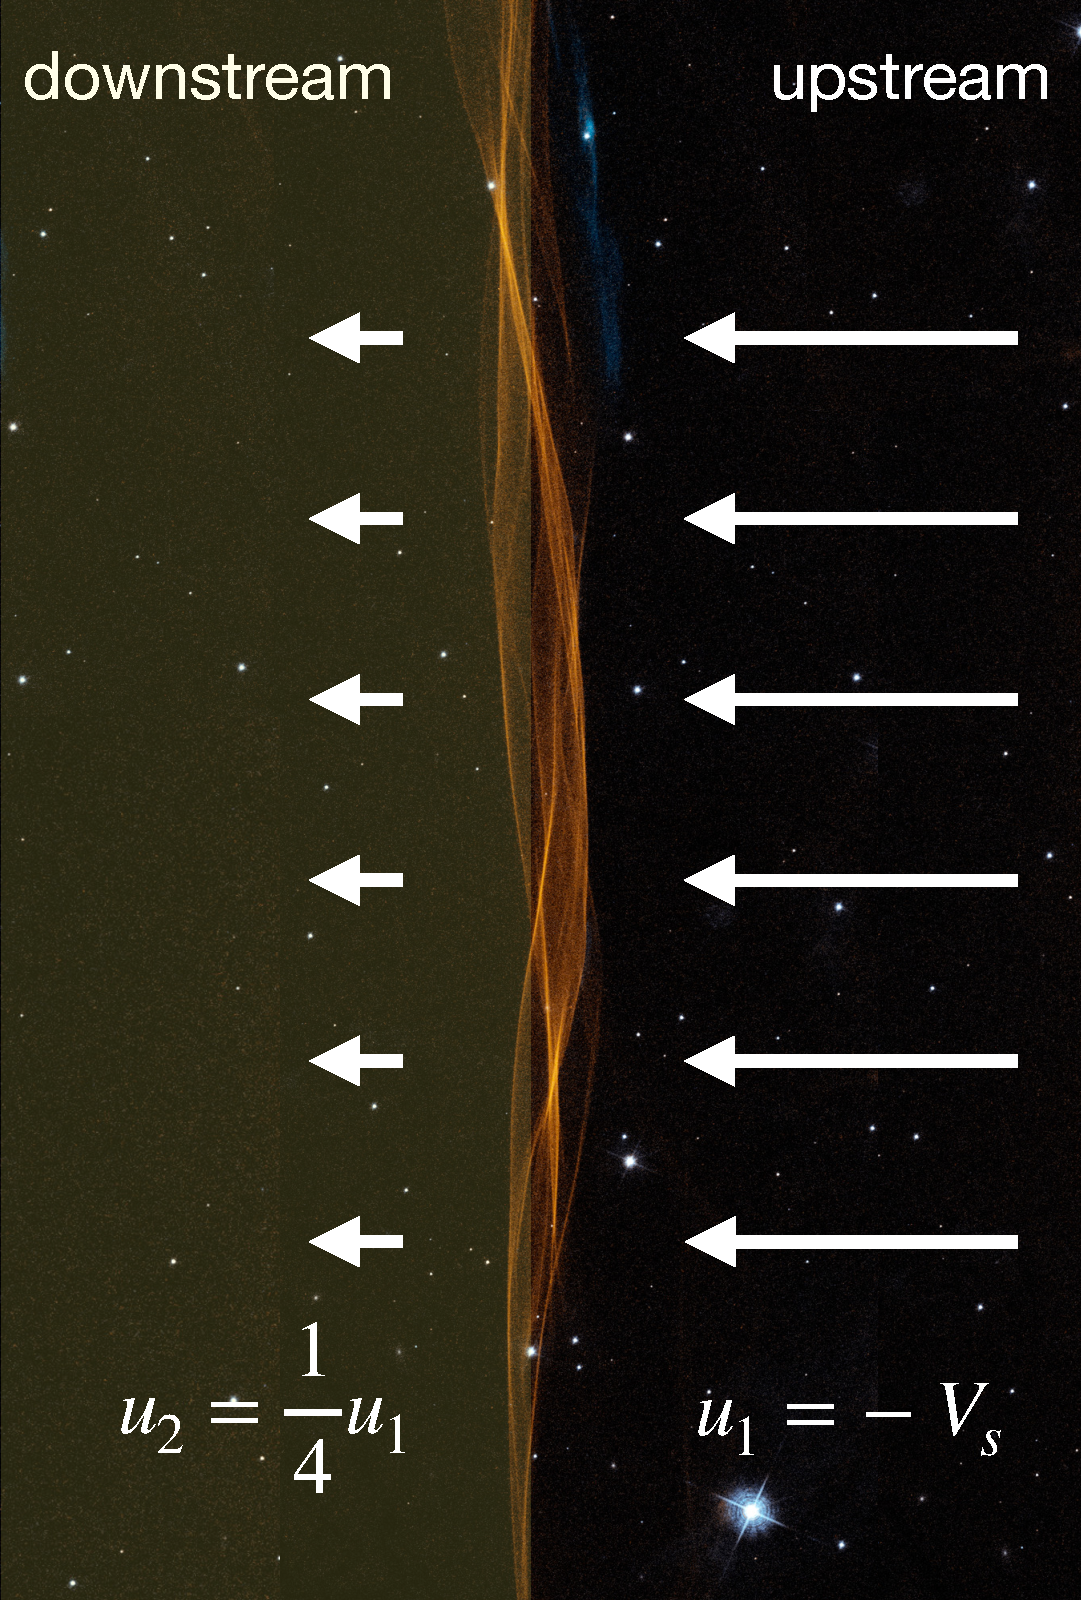
\includegraphics[width=0.31\textwidth]{figures/shockframe0.pdf} 
\hspace{\stretch{1}}
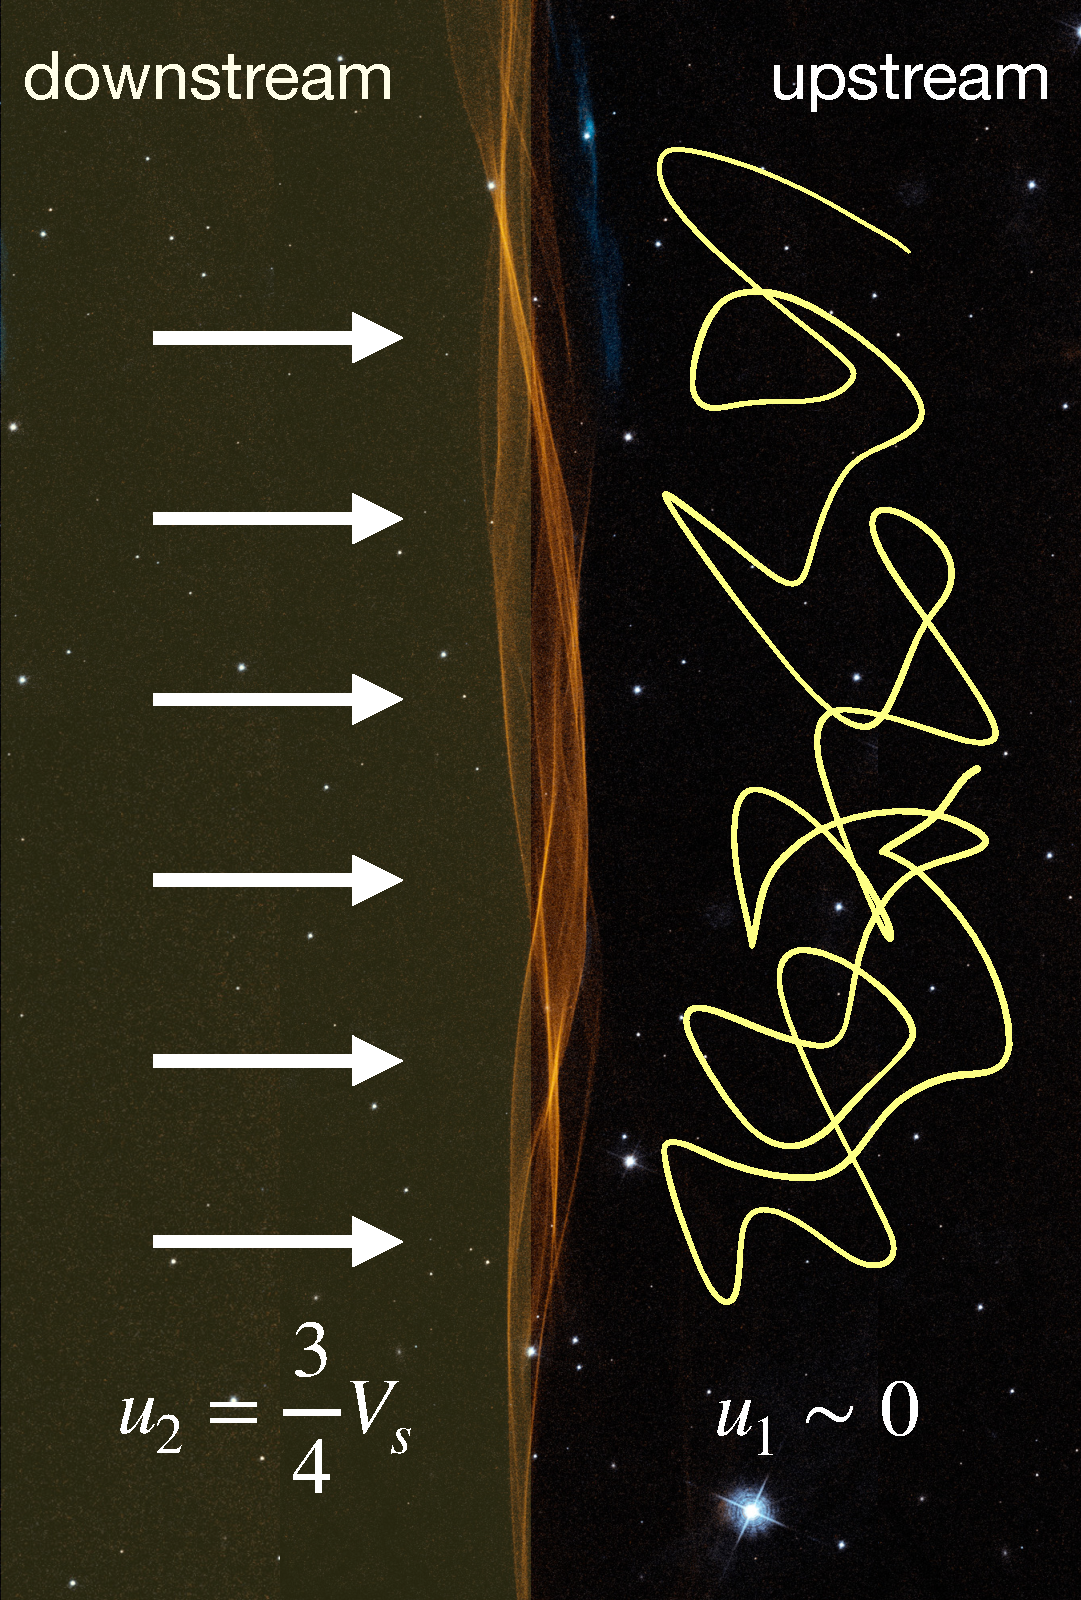
\includegraphics[width=0.31\textwidth]{figures/shockframe1.pdf} 
\hspace{\stretch{1}}
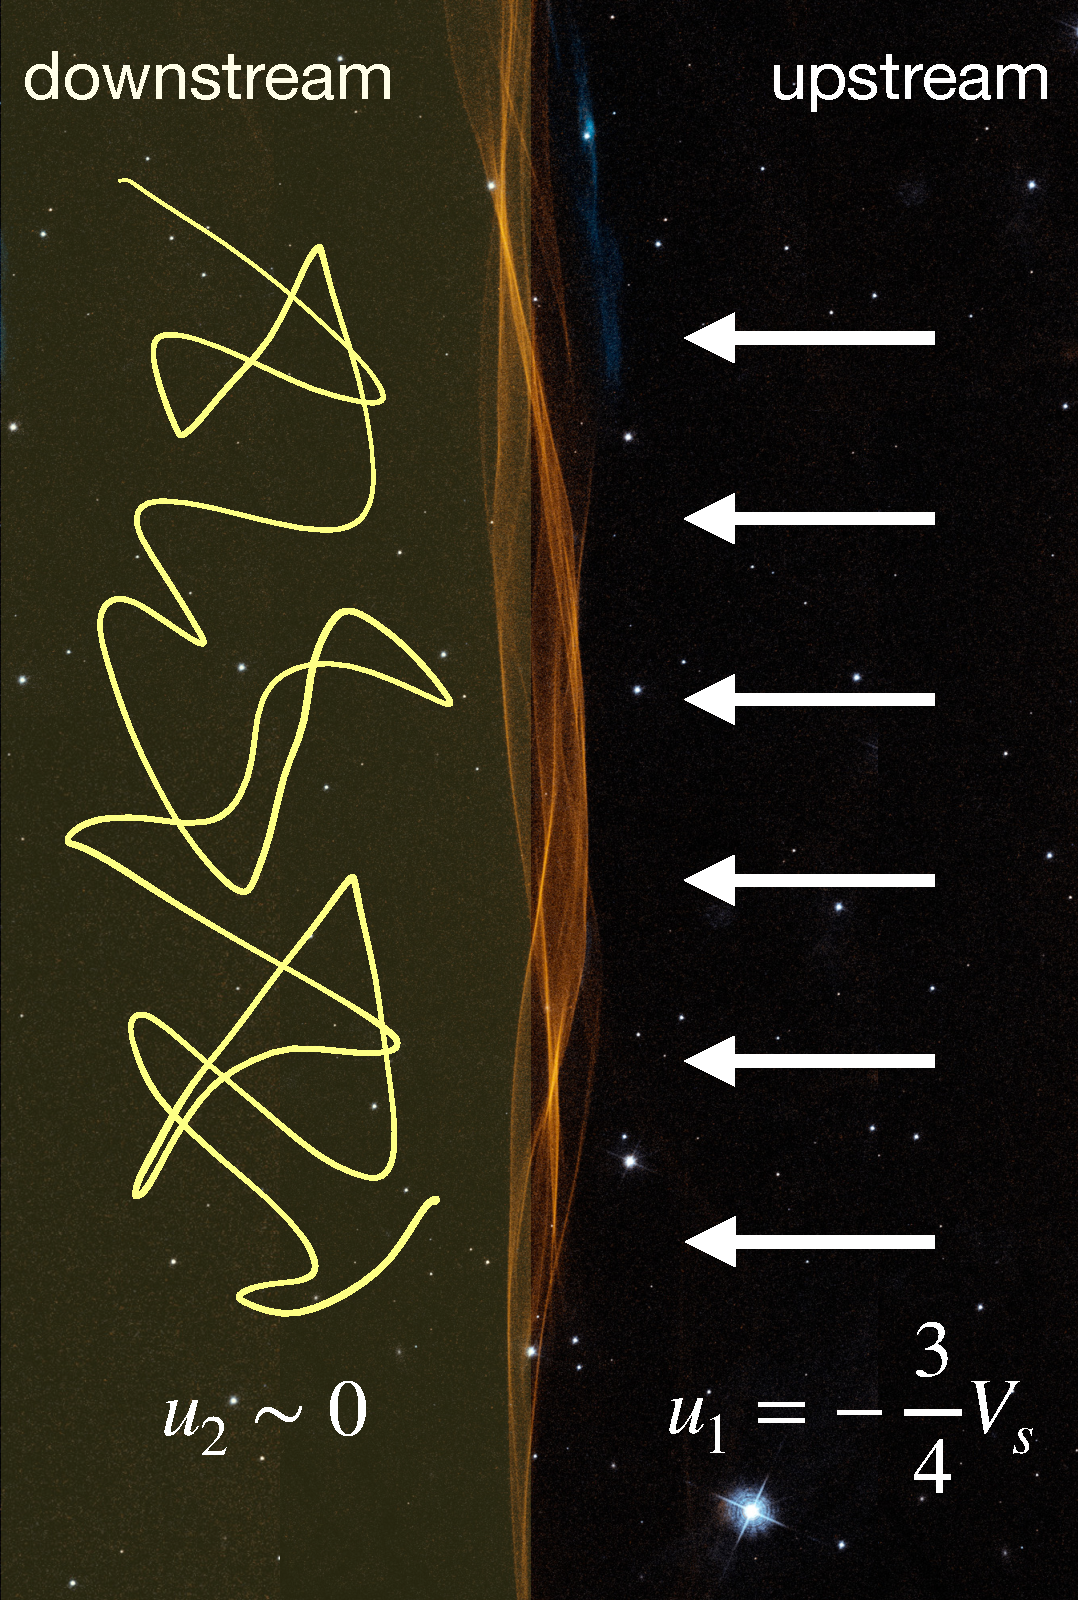
\includegraphics[width=0.31\textwidth]{figures/shockframe2.pdf} 
\caption{Illustration of plasma advection velocities across a shock (moving with velocity \( V_s \) in the Galaxy frame) in three different reference frames. Left panel: the shock is stationary. Center panel: the upstream plasma is stationary. Right panel: the downstream plasma is stationary.}\label{fig:shockframe}
\end{figure}

It is clear from this description that, for this process to occur effectively, particle directions need to be isotropized, which can happen through pitch-angle scattering by MHD waves. The generation of these waves is attributed to large-scale turbulence cascade downstream (injected by the SNR), and upstream by the energetic particles themselves (cosmic-ray streaming).
%
Additionally, it's crucial for particles to have a finite probability of escaping \emph{downstream} to fulfill the conditions of the generalized Fermi acceleration mechanism.

More quantitatively, consider now a particle in the upstream with initial energy \( E_i \). 
%
This particle diffuses and crosses the shock, and its energy in the downstream \( E_i^\prime \) can be calculated using Lorentz transformation:
%
\begin{equation}
E_i^\prime = \gamma E_i \left( 1 + \beta \mu_i \right)
\end{equation}
%
here, \( 0 \le \mu_i \le 1 \) and
%
\begin{equation}
\beta = \frac{u_u - u_d}{c} > 0~.
\end{equation}

The same principle applies to a particle transitioning from downstream to upstream, with the angle \( \mu_f^\prime \) having the opposite sign:
%
\begin{equation}
E_f = \gamma E^\prime_f (1 - \beta \mu_f^\prime)
\end{equation}
here, \( -1 \le \mu_f^\prime \le 0 \).

As a consequence, after completing a cycle (upstream $\rightarrow$ downstream $\rightarrow$ upstream), and assuming \( E^\prime_f \simeq E^\prime_i \), there is an overall gain in energy:
%
\begin{equation}
\frac{\Delta E}{E} = \frac{E_f - E_i}{E_i} = \overbrace{\gamma^2}^{\ge 1} \overbrace{(1 + \beta \mu_i)}^{\ge 1} \overbrace{(1 - \beta \mu_f^\prime)}^{\ge 1} - 1 > 0
\end{equation}

Notice that now, due to the different angular distributions, there are no configurations leading to an energy decrease, and \( \Delta E / E \) is \emph{always positive}.

To compute the mean energy gain over all the possible configurations, we have to compute the probability of a particle encountering the shock front with a specific pitch angle \( \mu \). 

Assuming \( n \) is the number density of isotropically distributed particles due to diffusion, this probability can be derived from the ratio of the flux of particles moving in the direction of \( \mu \) (\( J_\mu = n v \mu \)) to the total flux \( J \):
%
\begin{equation}
J = \int \frac{d\Omega}{4\pi} J_\mu = \frac{n v}{4\pi} \int_0^{2\pi} d\phi \int_0^1 d\mu \mu = \frac{n v}{4}
\end{equation}
%
where we use the information that only those particles with a projected \( \cos \theta > 0 \) will actually cross the shock front.

Therefore, the probability density is given by:
%
\begin{equation}
P(\mu) \propto \frac{n \mu v}{J} = 4 \mu
\end{equation}

To normalize \( P \) as a probability, we impose the condition:
%
\begin{equation}
\int_0^1 d\mu_i P(\mu_i) = 1 \rightarrow P(\mu_i) = 2\mu_i
\end{equation}
%
and
%
\begin{equation}
\int_{-1}^0 d\mu^\prime_f P(\mu^\prime_f) = 1 \rightarrow P(\mu^\prime_f) = -2\mu^\prime_f
\end{equation}

%It is evident that this probability is symmetric in both directions. 

Consequently, the average energy gain can be calculated as follows:
%
\begin{remark}
\begin{equation}\label{eq:firstorderxi}
\left\langle \frac{\Delta E}{E} \right\rangle_{\mu_i,\mu_f^\prime} \!\!\! = \! \int_0^1 \! d\mu_i \int_{-1}^0 \! d\mu^\prime_f \, P(\mu_i)P(\mu_f^\prime)\left[ \gamma^2(1+\beta\mu_i)(1-\beta\mu_f^\prime)-1 \right] 
\oset{\beta \sim 0}{\longrightarrow} \frac{4}{3} \beta 
%= \frac{4}{3} \left(\frac{u_u - u_d}{c} \right)
\end{equation}
\end{remark}

This result implies that the energy gain per cycle is \emph{first order} in $\beta$ as expected, for interstellar shock the resulting energy gain is of the order of \( 10^{-2}-10^{-3} \), which is enormously more than the second order mechanism! 

In assessing the efficiency of the proposed mechanism, we must additionally ensure that particles can effectively cross the shock in both directions. 
%s
In the upstream region, particles, regardless of the diffusion coefficient, will eventually encounter the shock front, which moves towards them at thousands of kilometers per second. Hence, the probability of crossing from upstream to downstream, \( P_{u \rightarrow d} \), is 1. Particles leave the upstream region only when their Larmor radius becomes larger than the accelerator's size or the maximum scale of the upstream turbulence.

In the downstream region, besides diffusion, we must consider that the plasma moves away from the shock, dragging particles with it. This leads to a finite probability of particles not returning to the shock front, finally resulting in a \emph{leakage}. 

To estimate this escape probability, we recall that the particle flux through an infinite planar shock is \( n v / 4 \), assuming efficient isotropization in the upstream. In the shock rest frame, there is a particle flow \( u_d n \) downstream, away from the shock front, which is lost to the acceleration process. Therefore, the escape probability is:
%
\begin{equation}
P_{d \rightarrow \infty} = \frac{u_d n}{n v / 4} \sim \frac{4 u_d}{c}
\end{equation}

The probability of return to the shock front is simply:
%
\begin{equation}\label{eq:pdtou}
P_{d \rightarrow u} = 1 - P_{d \rightarrow \infty} = 1 - \frac{4 u_d}{c}
\end{equation}

With \( u_d / c \sim 10^{-2} \), most particles from the downstream will return to the upstream. This results in a highly efficient first-order Fermi acceleration mechanism with a high probability of completing a cycle.

The existence of a small escape probability is crucial, as it leads to a distribution of energies rather than uniform acceleration. Applying equation~\eqref{eq:gammapescxi}, the slope of the \emph{differential spectrum}\footnote{The differential spectrum \( n(E)dE \) is  the number of particles with energy between \( E \) and \( E + dE \) thus \( E n(E) \propto E^{-\gamma} \)} produced by shock acceleration is given by the fractional energy gain (equation~\ref{eq:firstorderxi}) and the escape probability (equation~\ref{eq:pdtou}):
%
\begin{remark}
\begin{equation}
\gamma \simeq \frac{\frac{4}{3} \beta}{4 \frac{u_d}{c}} + 1 = \frac{3 u_d}{u_u - u_d} + 1 = \frac{r + 2}{r - 1} \rightarrow 2
\end{equation}
\end{remark}

We found that this mechanism results in a \emph{universal} power-law spectrum for strong shocks, as the slope depends only on the compression factor. Worth noticing, the accelerated spectrum is independent of the diffusion coefficient, which in turn depends on the poor-understood microphysics of particle-wave scattering.
%
On the other hand, the acceleration process's efficiency and the potential to accelerate particles to sufficiently high energies dramatically depend on the diffusion coefficient. 

\begin{figure}[t]
\centering
\includegraphics[width=0.6\textwidth]{figures/SNRspectra.pdf} 
\caption{Typical gamma-ray energy spectra for several of the most prominent SNRs. Young SNRs (e.g. Tycho) are shown in cyan. Solid lines show hadronic fits to the data. Adapted from~\cite{Funk2015}.}
\label{fig:snrspectra}
\end{figure}

%%% TO BE DONE 

To estimate the acceleration time, we need to consider the energy gain per crossing and the \emph{time taken for each cycle}.
%
The total cycle time is the sum of the times spent in the downstream and upstream\footnote{$
t_{\rm c, i} = \frac{\lambda_i}{\langle v_{x,i} \rangle} = \frac{\lambda_i}{-\int_0^{\pi/2} v_i \cos \theta d\cos\theta} = \frac{\lambda_i}{v_i / 2} \sim \frac{2\lambda_i}{c}$}:
%
\begin{equation}
\tau_{\rm cycle} = \frac{2\lambda_u}{c} + \frac{2\lambda_d}{c} %= \frac{4}{c} \left(\frac{D_1}{u_1} + \frac{D_2}{u_2}\right)
\end{equation}
%
where \( \lambda_i \) is the average distance traveled by a particle in each region.

The distance covered is obtained by computing the diffusion length \( \lambda_i \sim (2 D_i t_i)^{1/2} \) in the time spent by the advected plasma to catch the particle \( t_i \sim \lambda_i / u_i \), so we obtain
%
\begin{equation}
\langle \lambda_i \rangle = \frac{2 D_i}{u_i}
\end{equation} 
%
%{\color{red}where \( \lambda_i \) is the average distance traveled by a particle in each region is obtained by equating the diffusion length (\( l_{\text{d,i}} \simeq \sqrt{2 D_i t_i} \)) to the distance covered by the shock or the advected plasma.}

%%% END 

The characteristic acceleration timescale is then:
%
\begin{remark}
\begin{equation}
\tau_{\text{acc}} = \left( \frac{1}{E} \frac{dE}{dt} \right)^{-1} \sim \left( \frac{\Delta E}{E} \frac{1}{\tau_{\rm cycle}} \right)^{-1} \sim \frac{3}{u_u - u_d} \left( \frac{D_u}{u_u} + \frac{D_d}{u_d} \right) \oset{D_d \ll D_u}{\longrightarrow} 4 \frac{D_u}{u_u^2}
\end{equation}
\end{remark}

To compare this time with the age of the system, we use typical values for the upstream diffusion coefficient and the shock speed of a young SNR. For example, with \( D_u \simeq 10^{28}~\text{cm}^2~\text{s}^{-1} (E/\text{GeV})^{1/2} \) and \( u_u = 10^4 \) km/s, we find:
%
\begin{equation}
\tau_{\text{acc}} \simeq 1~\text{kyr}~\left( \frac{E}{\text{GeV}} \right)^{1/2} 
\end{equation}

However, observations of particles accelerated up to 100 TeV (see figure~\ref{fig:snrspectra}) in events like Tycho's supernova (age \( \sim 500 \) years) suggest that our estimates are off by orders of magnitude! Reconciling this discrepancy requires \emph{reducing} the diffusion coefficient in the upstream, possibly through cosmic-ray induced plasma instabilities. This leads to an inherently non-linear problem, underscoring the complexity of particle acceleration in astrophysical shocks.
\newpage

\chapter{Particle Transport in Galactic environments}
% !TEX root = ../lectures.tex
\section{The Grammage Pillar}
\label{sec:pillar}

\begin{figure}[t]
\centering
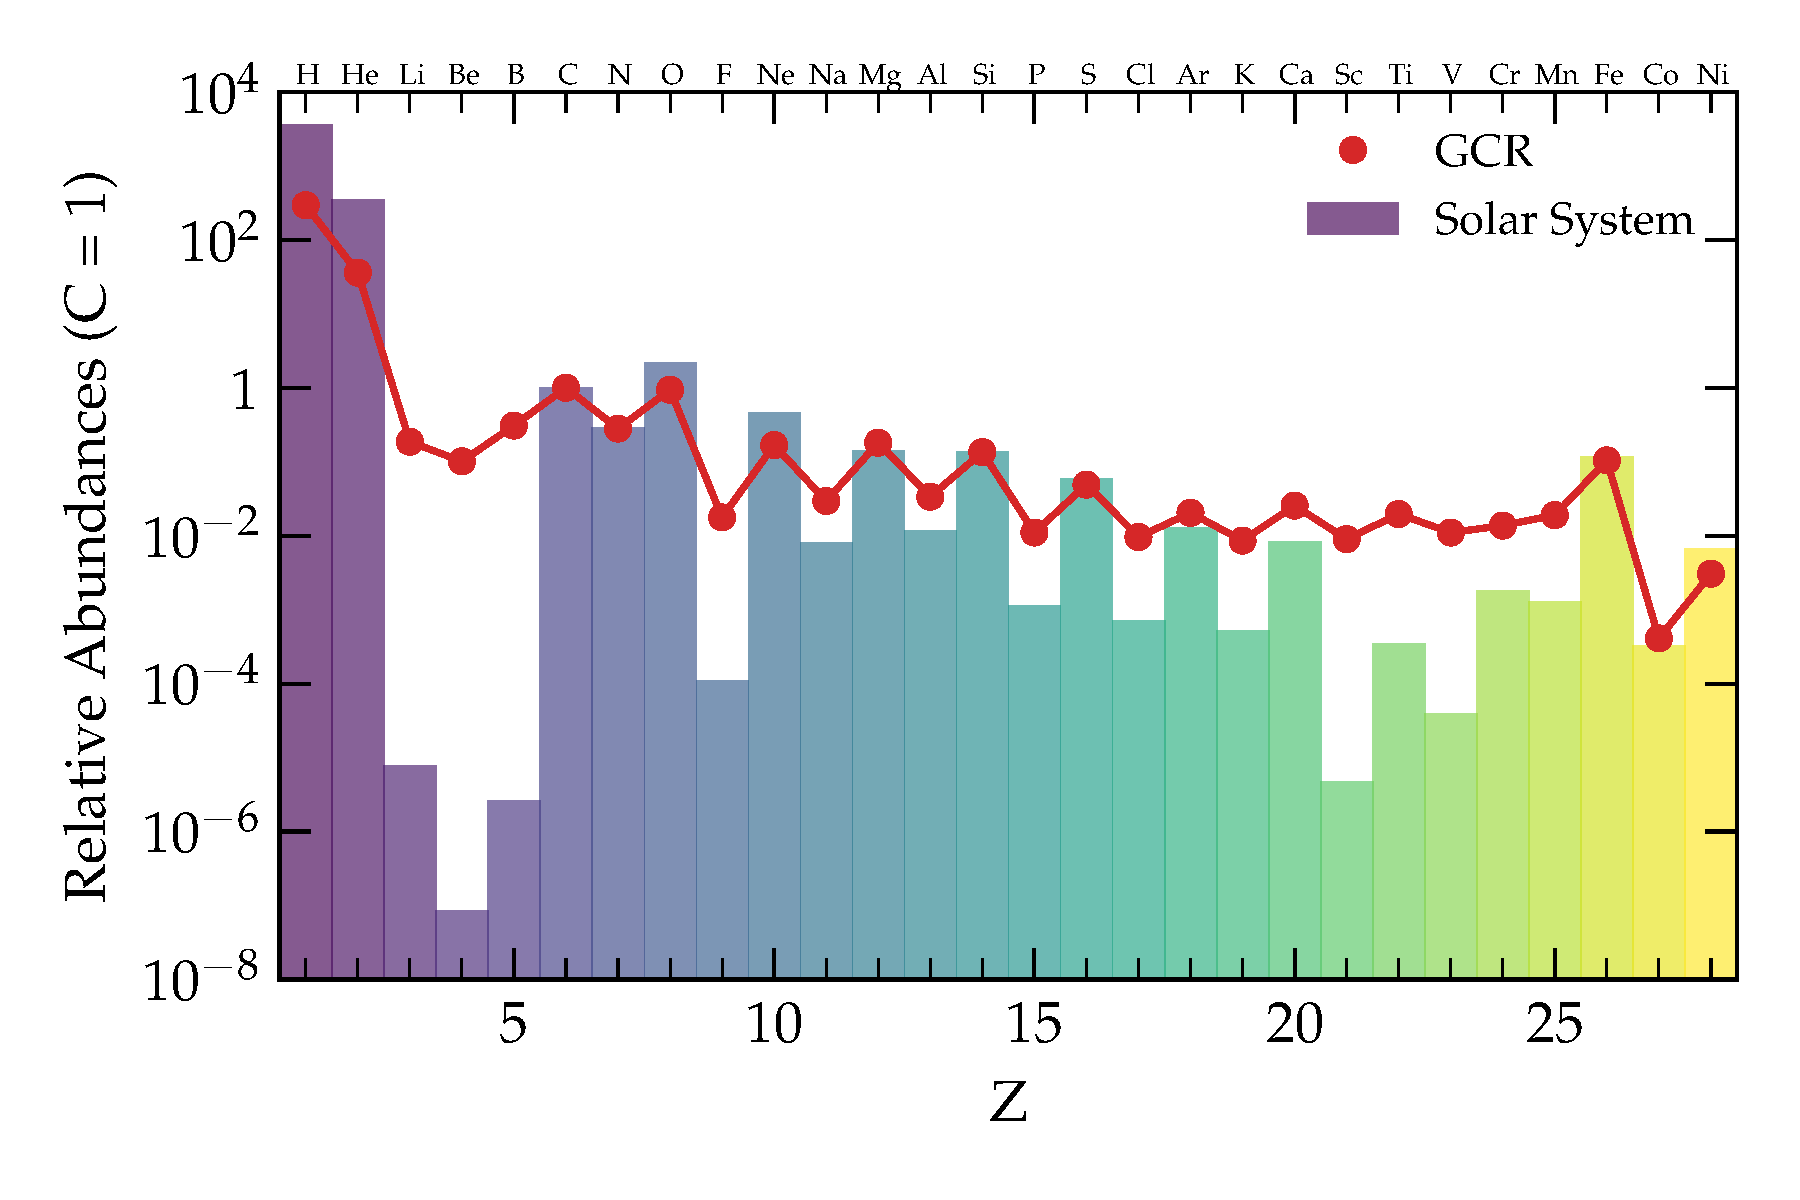
\includegraphics[width=0.6\textwidth]{figures/composition.pdf} 
\caption{Relative abundances of elements as a function of atomic number (Z) for Galactic Cosmic Rays (GCR)~\cite{} and the Solar System~\cite{}. The data highlight significant differences in the elemental composition between cosmic ray sources and the solar system medium, with abundances normalized to carbon (C=1).}
\label{fig:composition}
\end{figure}

The nuclear composition of cosmic rays (CRs) provides compelling evidence that GeV-TeV cosmic rays do not travel in straight lines but instead undergo a \emph{diffusive propagation} process. This conclusion arises from a detailed comparison between the isotopic composition of local CRs and that of the interstellar medium (ISM). This discovery\footnote{To the best of my knowledge, this idea was first introduced by Bradt and Peters in their 1950 paper published in \emph{Physical Review}.} is so fundamental to our understanding of CR propagation that it has been elevated to the status of a \emph{pillar} of cosmic ray physics.  

Figure~\ref{fig:composition} compares the isotopic composition of CRs observed locally~\cite{} with the abundances measured in the ISM surrounding the solar system (e.g., via absorption lines~\cite{}). While the overall isotopic abundances are broadly similar - suggesting that most CRs originate from the average ISM - some striking differences stand out. 
%
These differences are most evident for:  
%
\begin{itemize}
\item \emph{Light elements}: lithium (Li), beryllium (Be), and boron (B),  
\item \emph{Sub-iron elements}: scandium (Sc), titanium (Ti), and vanadium (V),  
\item Other anomalous species as nitrogen (N) and fluorine (F).  
\end{itemize}

In the ISM, these elements are present in negligible amounts compared to heavier nuclei like carbon (C) and oxygen (O). Specifically, Li, Be, and B are almost absent for two main reasons:  
\begin{itemize}
\item They are not efficiently produced in stars, as no stable nucleosynthesis pathways exist for these elements in stellar interiors, or during Big-Bang nucleosynthesis.  
\item They are fragile and are easily destroyed in high-temperature stellar environments through nuclear reactions such as \(\alpha\)-capture.  
\end{itemize}

However, the situation changes dramatically when looking at CRs where the abundances of Li, Be, and B in CRs are comparable to those of C and O. This discrepancy points to the existence of a \emph{secondary component}, which plays a key role in shaping the observed CR composition.  

This secondary component arises from the fragmentation of heavier primary nuclei (like C and O) into lighter nuclei (like Li, Be, and B) through \emph{spallation interactions} with the ISM gas. This process occurs as CRs propagate through the ISM and provides critical insight into their transport history.  

In fact, the observed ratios of secondary to primary nuclei, such as the boron-to-carbon (B/C) ratio, serve as \emph{tracers} of the cumulative amount of ISM material CRs have traversed. This material is quantified as the \emph{grammage} \(\chi\), which is the integrated column density of ISM along the CRs’ path:  
\begin{equation}
\chi = \int \! dl \, \rho(l),
\end{equation}
where \(\rho(l)\) is the ISM density along the trajectory \(l\).  

\subsection{Primary and Secondary Evolution Along the Grammage Path}

To clarify the interplay between primary and secondary nuclei, let us consider a simplified scenario involving one primary species (\(n_p\)) and one secondary species (\(n_s\)). Their abundances evolve along the grammage path \(\chi\), which reflects the cumulative amount of material traversed by CRs. Specifically:  

\begin{itemize}
\item The abundance of primary nuclei decreases due to inelastic collisions with ISM targets:  
\[
\frac{dn_p}{d\chi} = - \frac{n_p}{\lambda_p},
\]
where \(\lambda_p = m / \sigma_p\) is the \emph{interaction length} for the primary nuclei, \(m\) is the ISM target mass, and \(\sigma_p\) is the inelastic cross-section of the primary nuclei with ISM particles.  

\item Secondary nuclei are produced through spallation of the primary nuclei and are also depleted through their own interactions:  
\[
\frac{dn_s}{d\chi} = - \frac{n_s}{\lambda_s} + P_{p \rightarrow s} \frac{n_p}{\lambda_p},
\]
where \(P_{p \rightarrow s} = \sigma_{p \rightarrow s} / \sigma_p\) is the spallation probability for producing secondaries (\(s\)) from primaries (\(p\)).  
\end{itemize}

Assuming that no secondary nuclei are present initially (\(n_s = 0\) at \(\chi = 0\)), the secondary-to-primary ratio evolves with the grammage as:  
\begin{remark}
\begin{equation}\label{eq:grammagesimple}
\frac{n_s}{n_p} = P_{p \rightarrow s} \frac{\lambda_s}{\lambda_s - \lambda_p} \left[ \exp\left( -\frac{\chi}{\lambda_s} + \frac{\chi}{\lambda_p} \right) - 1 \right].
\end{equation}
\end{remark}  

This expression depends on measurable quantities, including the interaction lengths (\(\lambda_p\), \(\lambda_s\)) and the spallation probability (\(P_{p \rightarrow s}\)).

Among the secondary-to-primary ratios, the boron-to-carbon (B/C) ratio is the best-measured and provides the most precise constraints on CR propagation. Measurements by the AMS-02 experiment indicate a B/C ratio of approximately 0.3 for CRs with rigidities \(R \sim 10~\text{GV}\).  
%
On the other hand, laboratory measurements of the interaction lengths provides \( \lambda_{\rm C} \sim 9.1~\text{g/cm}^2 \), and \( \lambda_{\rm B} \sim 10.4~\text{g/cm}^2 \). Moreover, the spallation probability for carbon fragmenting into boron is estimated as \( P_{\rm C \rightarrow B} \sim 0.25 \)~\cite{}.

By combining these laboratory measurements with the AMS-02 observations, we deduce that CRs with rigidities \(R \sim 10~\text{GV}\) must have traversed a grammage of approximately:
\begin{equation}
\chi_{\rm ISM} \sim 10~\text{g/cm}^2.
\end{equation}

\begin{figure}[t]
\centering
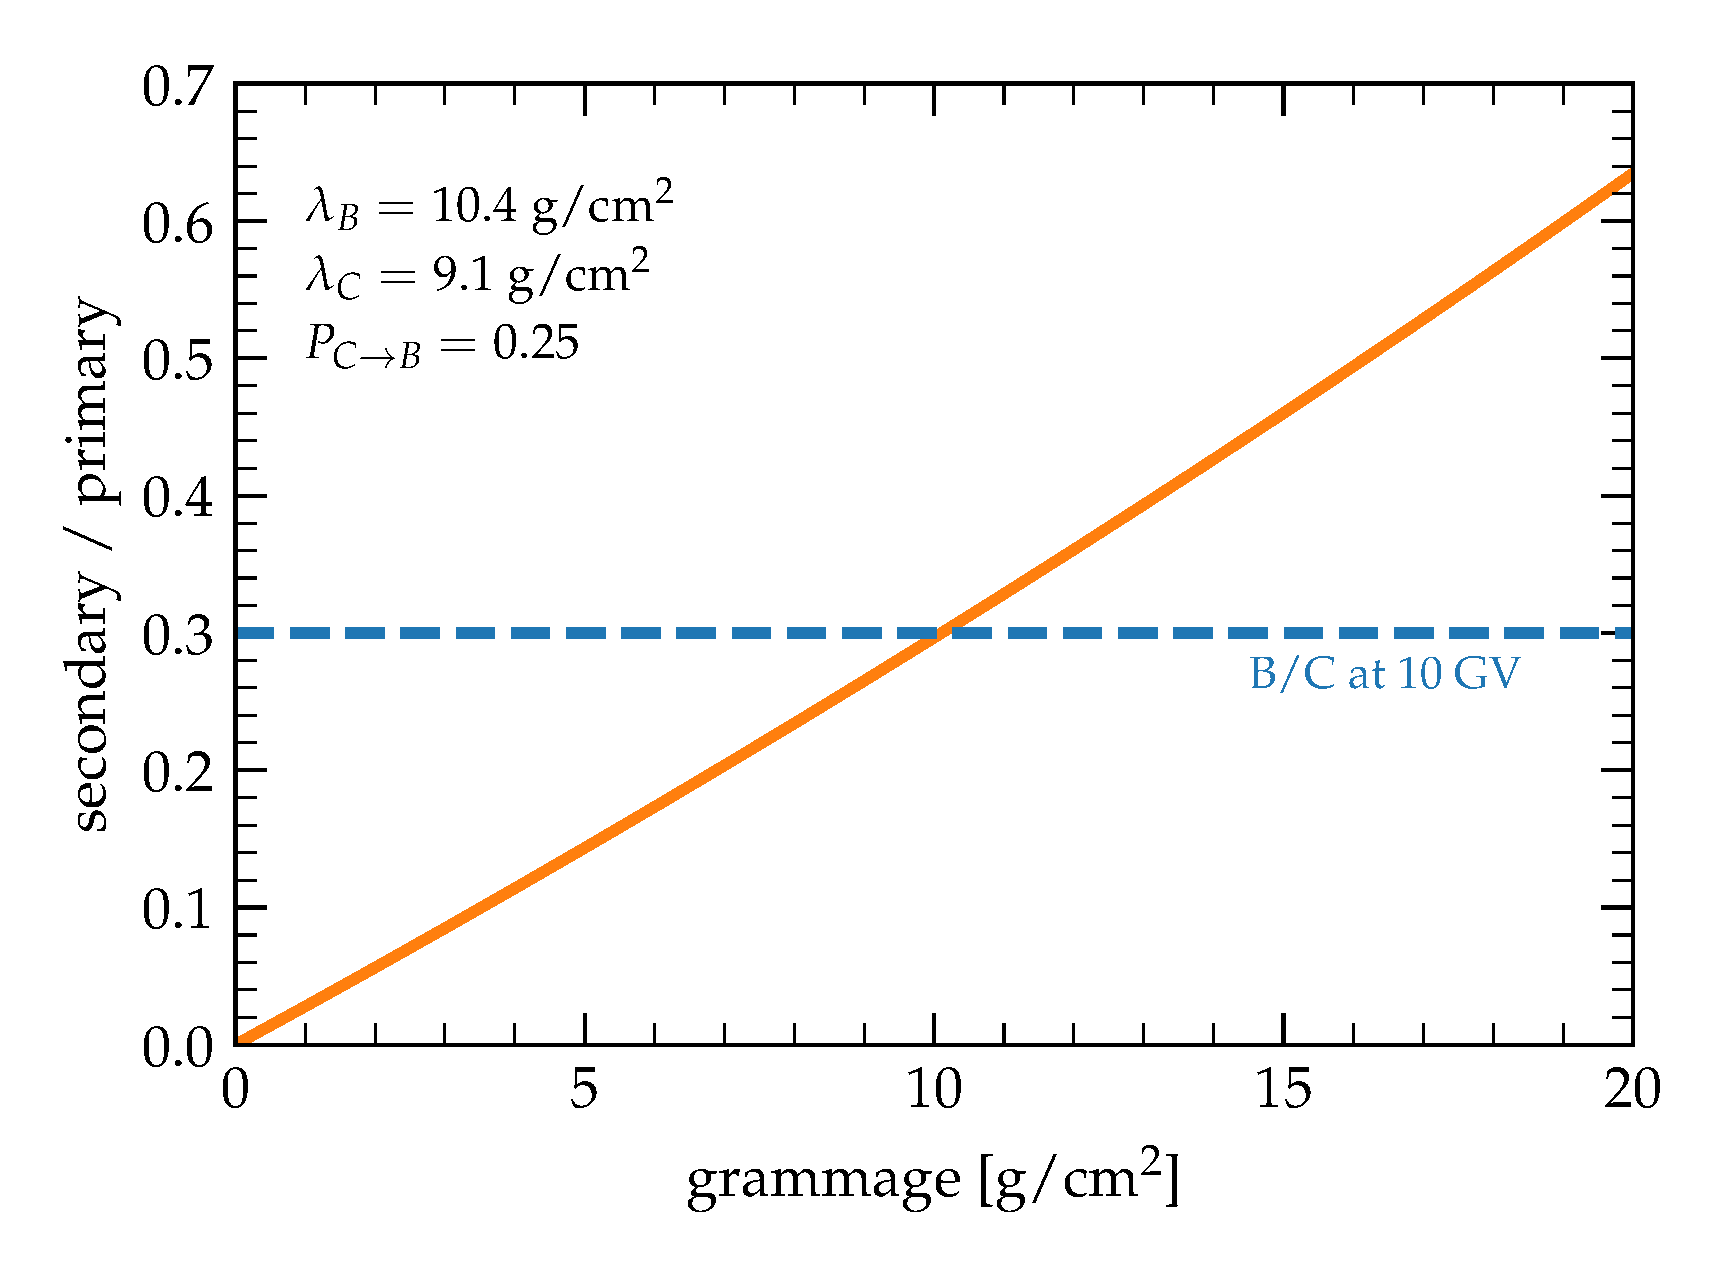
\includegraphics[width=0.6\textwidth]{figures/grammage_simple.pdf} 
\caption{The ratio of secondary to primary cosmic rays (B/C) as a function of grammage as in equation~\eqref{eq:grammagesimple}. The dotted blue line show the measurement by AMS-02 for CRs with rigidities \(R \sim 10~\text{GV}\).}
\label{fig:grammage10}
\end{figure}

\subsection{Galactic Disk Grammage and Confinement Time}

To estimate the grammage accumulated by CRs as they propagate, let us first compute the grammage associated with a single crossing of the Galactic gas disk, \(\chi_d\). This grammage is approximately the average surface density of the Galactic disk: \(\mu_d \sim 2.3 \times 10^{-3}~\text{g/cm}^2\).  

However, this value is significantly smaller than the \(\sim 10~\text{g/cm}^2\) inferred from the B/C ratio. This stark discrepancy indicates that CRs must traverse the disk \emph{multiple times} to accumulate the observed grammage.  

As such, to quantify the confinement time, we calculate the total time CRs need to cross the disk to accumulate the required grammage. This timescale is given by the number of crossings multiplied by the time for a single crossing:  
\[
\tau_{\rm conf} \gtrsim \frac{\chi_{\rm ISM}}{\chi_d} \frac{2h}{v} \sim 3 \times 10^6~\text{yr},
\]
where \(h \sim 100~\text{pc}\) is the half-thickness of the Galactic disk, and \(v \sim c\) is the approximate velocity of CRs.  

This \emph{minimum confinement timescale}, \(\tau_{\rm conf} \sim 3 \times 10^6~\text{yr}\), is several orders of magnitude longer than the time required for a CR to traverse the Galaxy in a straight line at the speed of light (a few tens of kiloyears for \(\sim 10~\text{kpc}\)). This vast difference provides compelling evidence for \emph{efficient confinement mechanisms} that cause CRs to propagate diffusively rather than ballistically through the Galaxy.  

The total residence time of CRs in the Galaxy can be independently estimated using radioactive isotopes such as \(^{10}\text{Be}\), which has a decay lifetime comparable to the timescale for CR leakage from the Galaxy. The ratio of radioactive \(^{10}\text{Be}\) to stable \(^{9}\text{Be}\) measured in CRs suggests a mean residence time of:  
\[
\tau_H \sim 10^8~\text{yr}.
\]  

Combining this estimate with the B/C ratio provides additional insights into CR propagation. To avoid exceeding the observed grammage, CRs must spend most of their time in the \emph{low-density Galactic halo}, where the density is much lower than in the disk. This requirement can be expressed as:  
\[
\langle \rho \rangle \lesssim \frac{\mu_d}{2h} \frac{\tau_h}{\tau_H}.
\]  
Here, \(\tau_h\) is the confinement time in the disk, and \(\tau_H\) is the total residence time in the Galaxy. This inequality implies that CRs interact predominantly with the disk during their brief crossings but spend the majority of their residence time in the halo.  

In conclusion, the composition of CRs, particularly the observed ratios of secondaries to primaries (e.g., B/C), provides robust evidence for efficient confinement mechanisms that ensure CRs propagate diffusively through the Galaxy. This confinement allows CRs to \emph{repeatedly return to the disk}, producing the observed secondary components, while spending most of their time in the low-density Galactic halo.

In the remainder of this chapter, we will explore transport models that explain these observations in terms of phenomenological quantities such as the diffusion coefficient and the size of the halo.  

% !TEX root = ../main.tex
%%%%%%%%%% SECTION %%%%%%%%%
\section{Cosmic-ray protons in the Galaxy}
\label{sec:protons}

The local density of CRs, their energy spectrum, and their relative abundances provide us with the only direct information we can obtain about CRs. These measurements, along with estimates of the CR column density deduced from diffuse $\gamma$-rays~\cite{Tibaldo2021universe, Grenier2015araa}, form the foundation for any model aiming to describe CR transport.
%
In this section, our goal is to construct a basic model for CR propagation in the Galaxy that enables us to extract from these observables valuable information on the injection of CRs and the subsequent processes they undergo in the ISM.

As discussed in \S~\ref{sec:intro}, the escape time of CRs is too long to be compatible with straight propagation along the large-scale magnetic field. Consequently, CRs must be confined to the Galaxy for a significant period of time, primarily spending most of their time in low-density gas regions, such as the Galactic halo.
%
The existence of such an extended (larger than the gas disc) magnetized region is supported by observations of synchrotron emission from edge-on external galaxies~\cite{Beck2015aar}.

To account for these crucial aspects, virtually all CR transport models rely on the same basic ideas: high-energy particles are accelerated in sources located in a thin disc region of thickness $h \sim 100$ pc, following an injected spectrum proportional to $E^{-\gamma}$, with $\gamma \gtrsim 2$ as expected in the presence of diffusive shock acceleration mechanism.

After the injection, CRs propagate diffusively throughout the Galactic halo, which has a scale height $H$ of approximately several kiloparsecs with a diffusion coefficient $D$ proportional to $E^\delta$, where $\delta \sim 1/3 - 1/2$, and they escape freely at the boundaries. The escape is an essential, yet poorly understood, process to guarantee the stationarity of the problem, and is usually simplified by setting the CR density to zero at the boundary $H$ above and below the Galactic plane~\cite{Ginzburg1980apss} (see figure~\ref{fig:galaxy}).

Since the size of the halo is much smaller than the Galaxy's radius ($R_{\rm d} \gtrsim 10$ kpc), a one-dimensional model is sufficient to describe the escape of CRs along the z-direction.

\begin{figure}[t]
\centering
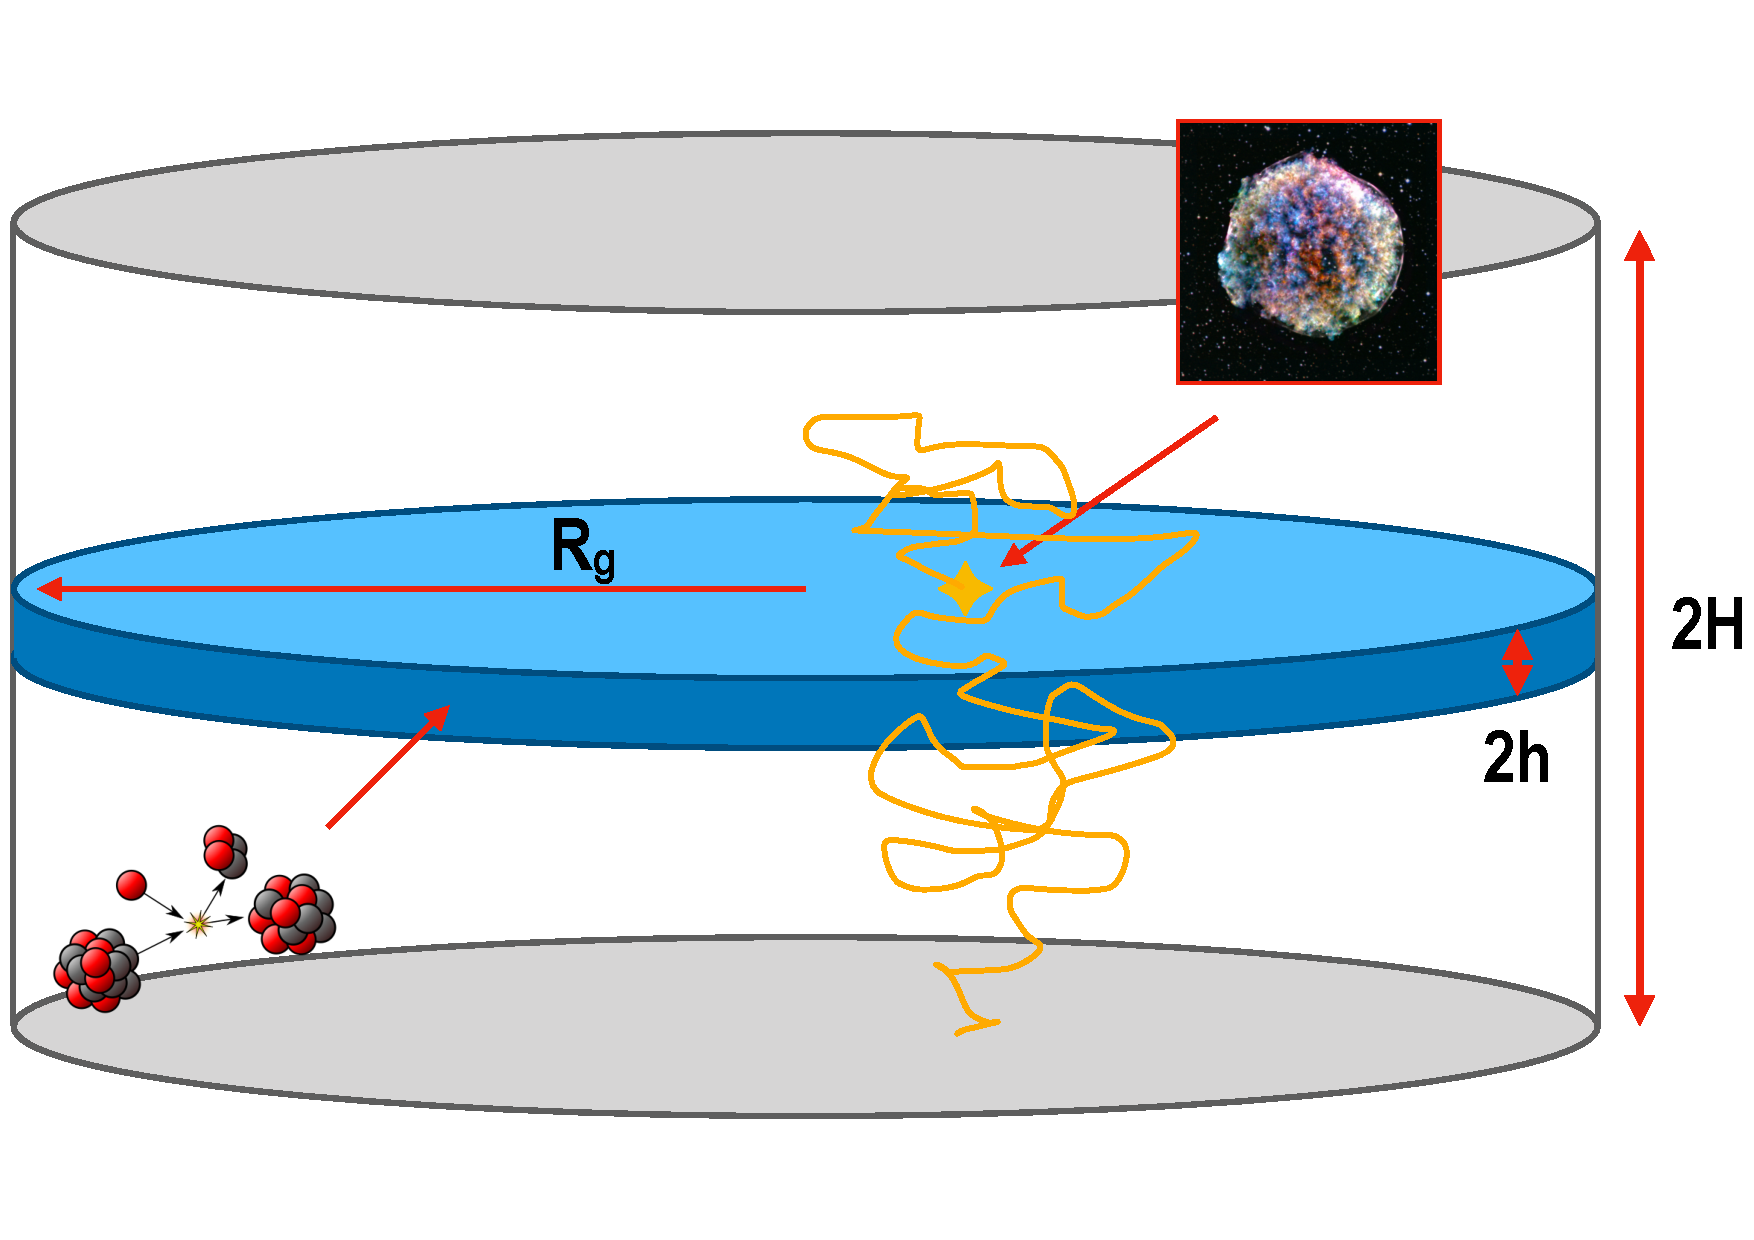
\includegraphics[width=0.6\textwidth]{figures/halo.pdf}
\caption{Illustrative depiction of the Milky Way's diffusive halo from the perspective of a cosmic ray physicist. Primary sources are distributed only in the disk. Also secondary nuclei emerge from cosmic ray interactions within the gaseous disk.}
\label{fig:galaxy}
\end{figure}

The simplest representation of this framework is achieved by employing the diffusion equation in the form of Fick's law~\cite{Fick1855}. 
%
It is important to note that one could also utilize the more general Fokker-Planck equation (see P.~Blasi's lecture notes in this volume). 
%
Both Fick's law and the Fokker-Planck equation are considered as purely phenomenological equations, as they represent different choices for the flux in the fundamental continuity equation.

In general, we can write the continuity equation with a source term $Q(E, z)$ as
%
\begin{equation}
\frac{\partial n}{\partial t} + \frac{\partial J}{\partial z} = Q
\end{equation}
%
where $n(E, z, t)$ is the CR number density per unit energy and $J$ the corresponding flux along $z$.

According to Fick's law of diffusion, the diffusive flux is determined by the concentration gradient as $J = -D \nabla n$. In other words, a spatial gradient in the particle density will give rise to a current that transports particles from regions of high density to regions of low density, with the magnitude of the current being proportional to the diffusion coefficient $D$. The dimensions of $D$ are then \emph{area per unit time}.

The diffusion equation becomes
%
\begin{equation}
\frac{\partial n}{\partial t} = \frac{\partial}{\partial z} \left( D\frac{\partial n}{\partial z} \right) + Q
\end{equation}

For a spatially constant diffusion coefficient we can derive the associated Green’s function as 
%
\begin{equation}
\mathcal G(z,t) = \left(\frac{1}{{4 \pi D t}}\right)^{1/2} {\rm e}^{-\frac{z^2}{4Dt}}
\label{eq:green}
\end{equation}
%
which we interpret as the probability for finding a particle that is injected at the disc ($z = 0$) at a position $z$ after the time $t$.

The mean distance from the Galactic plane can be calculated from equation~\eqref{eq:green}:
%
\begin{equation}
\langle z \rangle = \left(\frac{1}{{4 \pi D t}}\right)^{1/2} \int dz z {\rm e}^{-\frac{z^2}{4Dt}} \simeq \sqrt{Dt}
\end{equation}

The characteristic time to reach a height $\langle z \rangle = H$ can then be defined as  $t_{\rm H} \simeq H^2 / D$, and the characteristic averaged velocity with which CRs escape from the Galaxy as
%
\begin{equation}
v_{\rm D} \sim \frac{H}{t_{\rm H}} \sim \frac{D}{H}
\end{equation}

It is important to acknowledge that in order to obtain the average distance from the galactic plane, we made the assumption that the diffusion coefficient remains spatially constant throughout both the halo and the disc. However, due to the variations in gas densities and magnetic field strengths between these regions, this assumption may not hold true.

By adopting the phenomenological assumption of diffusion as the primary transport process, we can construct the CR evolution equation by specifying the source term assuming Galactic Supernovae (SNe) as major contributors.

Since the galactic disc is extremely thin with respect to the halo, we can describe the spatial part of the injection term as a delta-function $\delta(z)$, and therefore
%
\begin{equation}
Q(E,z) = \frac{\xi_{\rm CR} E_{\rm SN} \mathcal R_{\rm SN} N(E)}{\pi R_{\rm d}^2} \delta(z) 
\end{equation}
%
where $E_{\rm SN} \simeq 10^{51}$~erg is the SN kinetic energy, $\xi_{\rm CR}$ is the fraction of this energy converted in CR acceleration, $\mathcal R_{\rm SN} \simeq 1 / 50$~yr$^{-1}$ is the rate of SNe in the Galaxy and $N(E)$ the spectrum of one SN. 

Considering that our Galaxy has an age of several billion years and observations of light elements suggest that CRs spend at most a hundred million years within our Galaxy, it can be concluded that the dynamical timescale of the Galaxy is significantly longer than the phenomena we are investigating. Therefore, we are justified in assuming stationarity, and the diffusion equation for protons $n_p$ becomes:
%
\begin{equation}
-\frac{\partial}{\partial z}\left[ D(E) \frac{\partial n_p}{\partial z}\right] = \frac{\xi_p E_{\rm SN} \mathcal R_{\rm SN}}{\pi R_{\rm d}^2} N(E) \delta(z)
\label{eq:protons}
\end{equation}

For $z \ne 0$, and imposing the boundary conditions $n_p(z = \pm H, E) = 0$, it gives the solution\footnote{The general solution to the differential equation can be written as $n_p(z)=A+Bz$:
\begin{itemize}
\item For $z>0$, we impose $n_p(H)=0$ which gives $n_p(z)=A\left(1-\frac{z}{H}\right)$
\item For $z<0$, we impose $n_{\rm p}(-H)=0$ which gives $n_{\rm p}(z)=A\left(1+\frac{z}{H}\right)$
\end{itemize}
Combining the two regions and imposing $n_p(0)=n_0(E)$, we obtain the solution valid in both regions as in equation~\eqref{eq:nzwithabs}.}:
%
\begin{equation}
D \frac{\partial n_p}{\partial z} = \text{Constant} \, \longrightarrow \, n_p(z) = n_0(E) \left( 1 - \frac{|z|}{H} \right)
\label{eq:nzwithabs}
\end{equation}

Thereby the diffusive flux is found to be constant in $z$, and we can compute it at the disc $z = 0$ as:
%
\begin{equation}
\left. D \frac{\partial n_p}{\partial z}\right|_{z=0^+} = - D \frac{n_{0}}{H}
\label{eq:flux}
\end{equation}

To find the density $n_0$ we integrate the diffusion equation around $z=0$:
%
\begin{equation}
\lim_{\epsilon\rightarrow0} \int_{\epsilon^-}^{\epsilon^+} \!\!\! dz 
\left\{ -\frac{\partial}{\partial z} \left[ D \frac{\partial n_p}{\partial z} \right] = Q(E,z) \right\} 
\end{equation}
%
which leads to
%
\begin{equation}
\left. -2D \frac{\partial n_p}{\partial z}\right|_{z=0^+} = \frac{\xi_p E_{\rm SN} \mathcal R_{\rm SN}}{\pi R_{\rm d}^2} N(E) 
\end{equation}
%
and using the equation for the flux derived in equation~\eqref{eq:flux}:
%
\begin{equation}
n_p(E) = \frac{\xi_p E_{\rm SN} \mathcal R_{\rm SN} N(E)}{2 \pi R_{\rm d}^2}  \frac{H}{D(E)} 
\label{eq:protonsimplesolution}
\end{equation}

\begin{figure}[t]
\centering
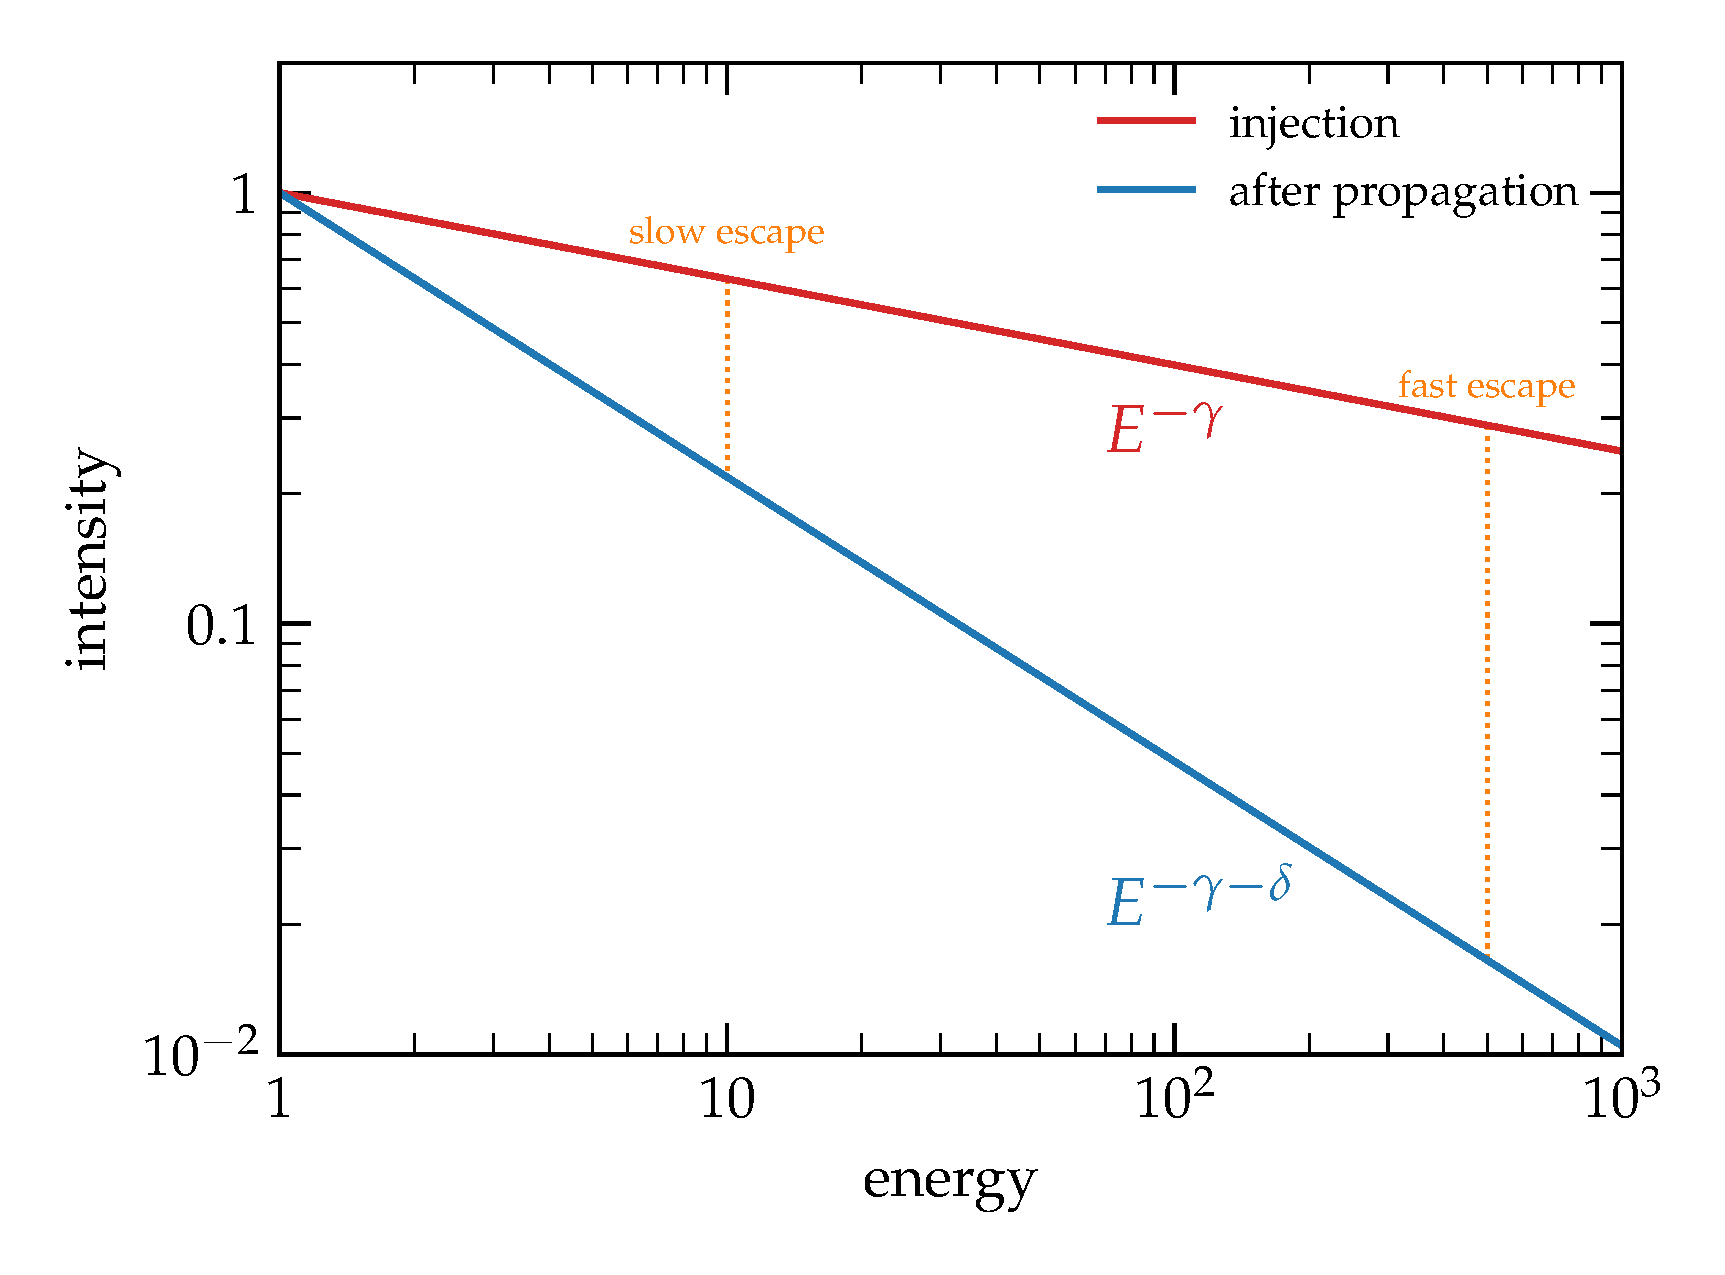
\includegraphics[width=0.6\textwidth]{figures/diffusion_softening.pdf}
\caption{Comparison between the \emph{injection spectrum} and the \emph{propagated spectrum} within an energy-dependent \emph{diffusion} toy-model. Higher-energy particles escape more swiftly, leading to a reduced equilibrium intensity. Consequently, the propagated spectrum consistently exhibits a \emph{steeper} profile than the injected counterpart.}
\label{fig:softening}
\end{figure}

As a result, we have obtained the CR spectrum as measured by an observer placed within the galactic disc.
%
It can be simply re-written as:
%
\begin{equation}
n_p(E) = \frac{Q_{\rm SN}(E) \tau_{\rm esc}(E)}{V_{\rm G}}
\end{equation}
%
where $Q_{\rm SN}(E) = \xi_p E_{\rm SN} \mathcal R_{\rm SN} N(E)$ is the number of particles injected per unit time by all supernovae, $\tau_{\rm esc} = H^2/D$ is the escape time, and $V_{\rm G} = 2\pi R_{\rm d}^2H$ is the total volume of the Galaxy.

In summary, since the diffusion coefficient increases with energy, following a power-law dependence as $D \propto E^{\delta}$, the escape time scales $\tau_{\rm esc} \propto E^{-\delta}$, and the spectrum we observe is always \emph{steeper} than the spectrum produced at the CR sources.

In point of fact, assuming that the sources inject in the ISM a power-law spectrum $E^{-\gamma}$, what we measure is a spectrum proportional to $E^{-\gamma-\delta}$ since high-energy particles spend less time in the Galaxy compared to lower-energy particles, resulting in a significant suppression of their density relative to the low-energy part of the spectrum.
%
This is depicted in figure~\ref{fig:softening}. 

It is important to note that since what we observe is a combination of the injection and transport processes, any deviation from a pure power-law in the observed spectrum of protons (or any primary species) cannot be easily disambiguate if due to propagation or acceleration effects. 

Finally, it is interesting to make some remarks on the assumptions we have made so far.  
%
The physics of CR transport is influenced not only by diffusion but also by boundary conditions\footnote{Further exploration of this subject is provided in the lecture notes by P.~Blasi within the same volume.}.
%
As discussed earlier, the condition of free escape, where $n(z = \pm H, E) = 0$, implies that the diffusion current does not depend on position.

At the boundary, conservation of flux requires:
%
\begin{equation}
\left. D \frac{\partial n}{\partial z} \right|_{z=H} = \frac{c}{2} n_{\rm out} %\, \longrightarrow \, n_{\rm out} = \frac{3D}{cH} n_0 \sim \frac{\lambda(E)}{H} n_0 \ll n_0
\end{equation}
%
where it is assumed that particles outside the diffusing volume are streaming away approximately at the speed of light\footnote{The flux outgoing a semi-finite plane is $\Phi = \int_0^1 d\mu \mu v n \simeq n c \int_0^1 d\mu \mu$, where $\mu$ is the cosine of the incident angle.},~$c$.

On the other hand, we can express $D$ in terms of the mean free path $\lambda$ as $D = \frac{1}{3} c \lambda$\footnote{A plain  derivation of this expression is provided in Sec.~3.2 of~\cite{Kachelriess2008arxiv}}, yielding:
%
\begin{equation}
n_{\rm out} = \frac{2D}{cH} n_0 \sim \frac{\lambda(E)}{H} n_0 % \ll n_0
\end{equation}

The condition of free-escape $n_{\rm out} \ll n_0$ is then satisfied as long as the path lenght $\lambda$ is much smaller than $H$, which remains true for $E \ll $~PeV~\cite{Blasi2019prl}. 

Despite the great importance of this assumption we do not have any knowledge on what determines the halo size or whether the halo size depends on energy or space (see however~\cite{Evoli2018prl,Dogiel2020apj} for an attempt to model the halo based on physical principles).

In the formulation of the transport equation for protons, we have initially disregarded the nuclear energy losses. For protons, the primary energy loss mechanism is the inelastic scattering with proton target leading to pion production. This process is characterized by a typical cross section of approximately $\sigma_{\rm pp}\sim 3\times 10^{-26}$ cm$^2$.

Nevertheless, when considering the timescale of this process in the ISM with a typical density of $n_{\rm d} \sim 1$ cm$^{-3}$, we find:
%
\begin{equation}
\tau_{\rm pp} \simeq \frac{1}{\bar{n}\sigma_{\rm pp}c} \simeq \, \text{Gyr}
\end{equation}

Here, $\bar{n} = n_{\rm d} h/H$ represents the average density within the diffusive volume.

From this calculation, we observe that the timescale for $pp$ scattering is significantly long, on the order of a Gigayear. Consequently, we can confidently assume that this process does not significantly alter the spectrum of propagated protons. 

However, despite being subdominant in terms of energy losses, the proton-proton interaction resulting in neutral pions that decay into two $\gamma$-rays is the leading mechanism for production of the spectacular diffuse emission observed along the Galactic Plane in Fermi-LAT data above $\sim 100$~MeV (see P.D.~Serpico's lecture notes in this volume).

On the other hand, the interaction cross-section becomes increasingly relevant when dealing with heavy nuclei. Therefore, in \S\ref{sec:nuclei}, we will discuss the incorporation of these effects in the transport of nuclei through the ISM.

%%%%%%%%%% SECTION %%%%%%%%%%
\section{Primary nuclei}
\label{sec:nuclei}

Energy losses resulting from the fragmentation of nuclei in the ISM play a critical role in the propagation of CR nuclei across the Galaxy. It is worth noting that other loss mechanisms, such as ionization and Coulomb interactions, are only relevant for energies $T \lesssim 10$ GeV/n, and therefore, we will neglect them in the remainder of these lecture notes (see P.D.~Serpico's lecture notes in this volume).

When accounting for these losses, the transport equation for the phase-space distribution function\footnote{See appendix~\ref{app:intensity} for the formal definition of this quantity.} of a species $\alpha$ takes the following form:
%
\begin{equation}
-\frac{\partial}{\partial z} \left[ D_\alpha(p) \frac{\partial f_\alpha}{\partial z} \right] = 
Q_\alpha(p) \delta(z) - \frac{f_\alpha}{\tau_{\rm f, \alpha}} + \sum_{\alpha^\prime > \alpha}  \frac{f_{\alpha^\prime}}{\tau_{\rm f, \alpha\alpha^\prime}}
\end{equation}

In this equation, the source term $Q_\alpha(p)$ is now accompanied by a \emph{sink} term, which accounts for the spallation of CR nuclei. The rate of spallation is proportional to the spallation cross section $\sigma_\alpha$ and the density of the interstellar gas in the disc $n_{\rm d}$. Additionally, the last term on the right-hand side represents the source term due to the spallation of heavier nuclei of type $\alpha^\prime$ into nuclei of type $\alpha$. In that regard, the quantities $\tau_{\rm f, \alpha\alpha^\prime}$ contain the branching ratio of spallation of $\alpha^\prime$ into $\alpha$.

As the target gas for nuclear fragmentation is confined to the thin disk, we can explicitly define the timescale for inelastic losses as
%
\begin{equation}
\frac{1}{\tau_{\rm f, \alpha}} = 2 h n_{\rm d} \delta (z) c \sigma_\alpha
\label{eq:scalingcs}
\end{equation}
%
Additionally, we assume that spallation cross-sections are energy-independent. Interestingly, measurements of spallation cross-sections above a few GeV/n do not show any appreciable dependence on the projectile energy~\cite{Evoli2019prd}.

On the other hand, the cross sections of various elements increase with the atomic mass number, roughly following a geometric scaling law~\cite{Letaw1983apjs}:
%
\begin{equation}
\sigma_\alpha \simeq 45 \, \text{mb} \, A^{2/3}
\end{equation}

The source term is defined by assuming that particles are injected relativistically, $p \gtrsim p_{\rm min} = A m_p c$, with a power-law momentum distribution $p^{-\gamma}$:
%
\begin{equation}
Q_\alpha(p, z) = Q_{0,\alpha} \left(\frac{p}{p_{\rm min}}\right)^{-\gamma} \delta (z) 
\end{equation}

To determine the normalization factor, $Q_{0,\alpha}$, we impose that the total luminosity in CRs equals that released by Galactic SNe:
%
\begin{equation}
\xi_{\rm CR} E_{\rm SN} \mathcal R_{\rm SN} = \int \! dV \! \int \! d^3 \! p \, E(p) Q(z,p)
\end{equation}

This results in
%
\begin{equation}
Q_{0,\alpha} = \frac{(\gamma - 4) c^3 \xi_{\rm CR} E_{\rm SN} \mathcal R_{\rm SN}}{4 \pi^2 R_{\rm d}^2 E_{\rm min}^4}
\end{equation}
%
where $E_{\rm min} = p_{\rm min} c$.

The transport equation for a pure primary species, i.e., without a significant secondary contribution, can be written as
%
\begin{equation}
-\frac{\partial}{\partial z} \left[ D_\alpha(p) \frac{\partial f_\alpha}{\partial z} \right] = Q_{0,\alpha}(p)\delta(z) - 2 h n_{\rm d} \delta (z) c \sigma_\alpha f_\alpha(p)
\label{eq:primary}
\end{equation}

We notice that this equation can be solved in the same way and with the same boundary conditions at $z = \pm H$ as equation~\eqref{eq:protons}. For $z \neq 0$, it gives:
%
\begin{equation}
f_\alpha(z,p) = f_{0,\alpha}(p) \left( 1 - \frac{|z|}{H} \right)
\end{equation}

The expression of $f_{0,\alpha}(p)$ can be obtained by integration of equation~\eqref{eq:primary} around the disc
%
\begin{equation}
\left. -2 D_\alpha \frac{\partial f_\alpha}{\partial z} \right|_{0+} = Q_{0,\alpha}(p) - 2 h n_{\rm d} c \sigma_{\alpha} f_{0,\alpha}(p)
\end{equation}

Finally, we find:
%
\begin{equation}
f_{0,\alpha}(p) = \frac{Q_{0,\alpha} H}{2D_\alpha} \frac{1}{1 + n_{\rm d} \frac{h}{H} c \sigma_{\alpha} \frac{H^2}{D_\alpha}}
\end{equation}

Notice that $\bar n = n_{\rm d} h/H$ represents the \emph{average} density experienced by CRs during their Galactic propagation, while $H^2/D_\alpha$ denotes their diffusion time, and $1/(\bar n c \sigma_\alpha)$ represents the effective spallation time.

To express this in terms of the matter thickness traversed by CRs during their propagation, we introduce the concept of grammage, denoted as 
%
\begin{equation}
\rchi(p) = m_{\rm p} \left( n_{\rm d} \frac{h}{H} \right) c \left( \frac{H^2}{D_\alpha} \right) \sim m_p \bar n c \tau_{\rm esc}(p)
\label{eq:grammage}
\end{equation}

\begin{figure}[t]
\centering
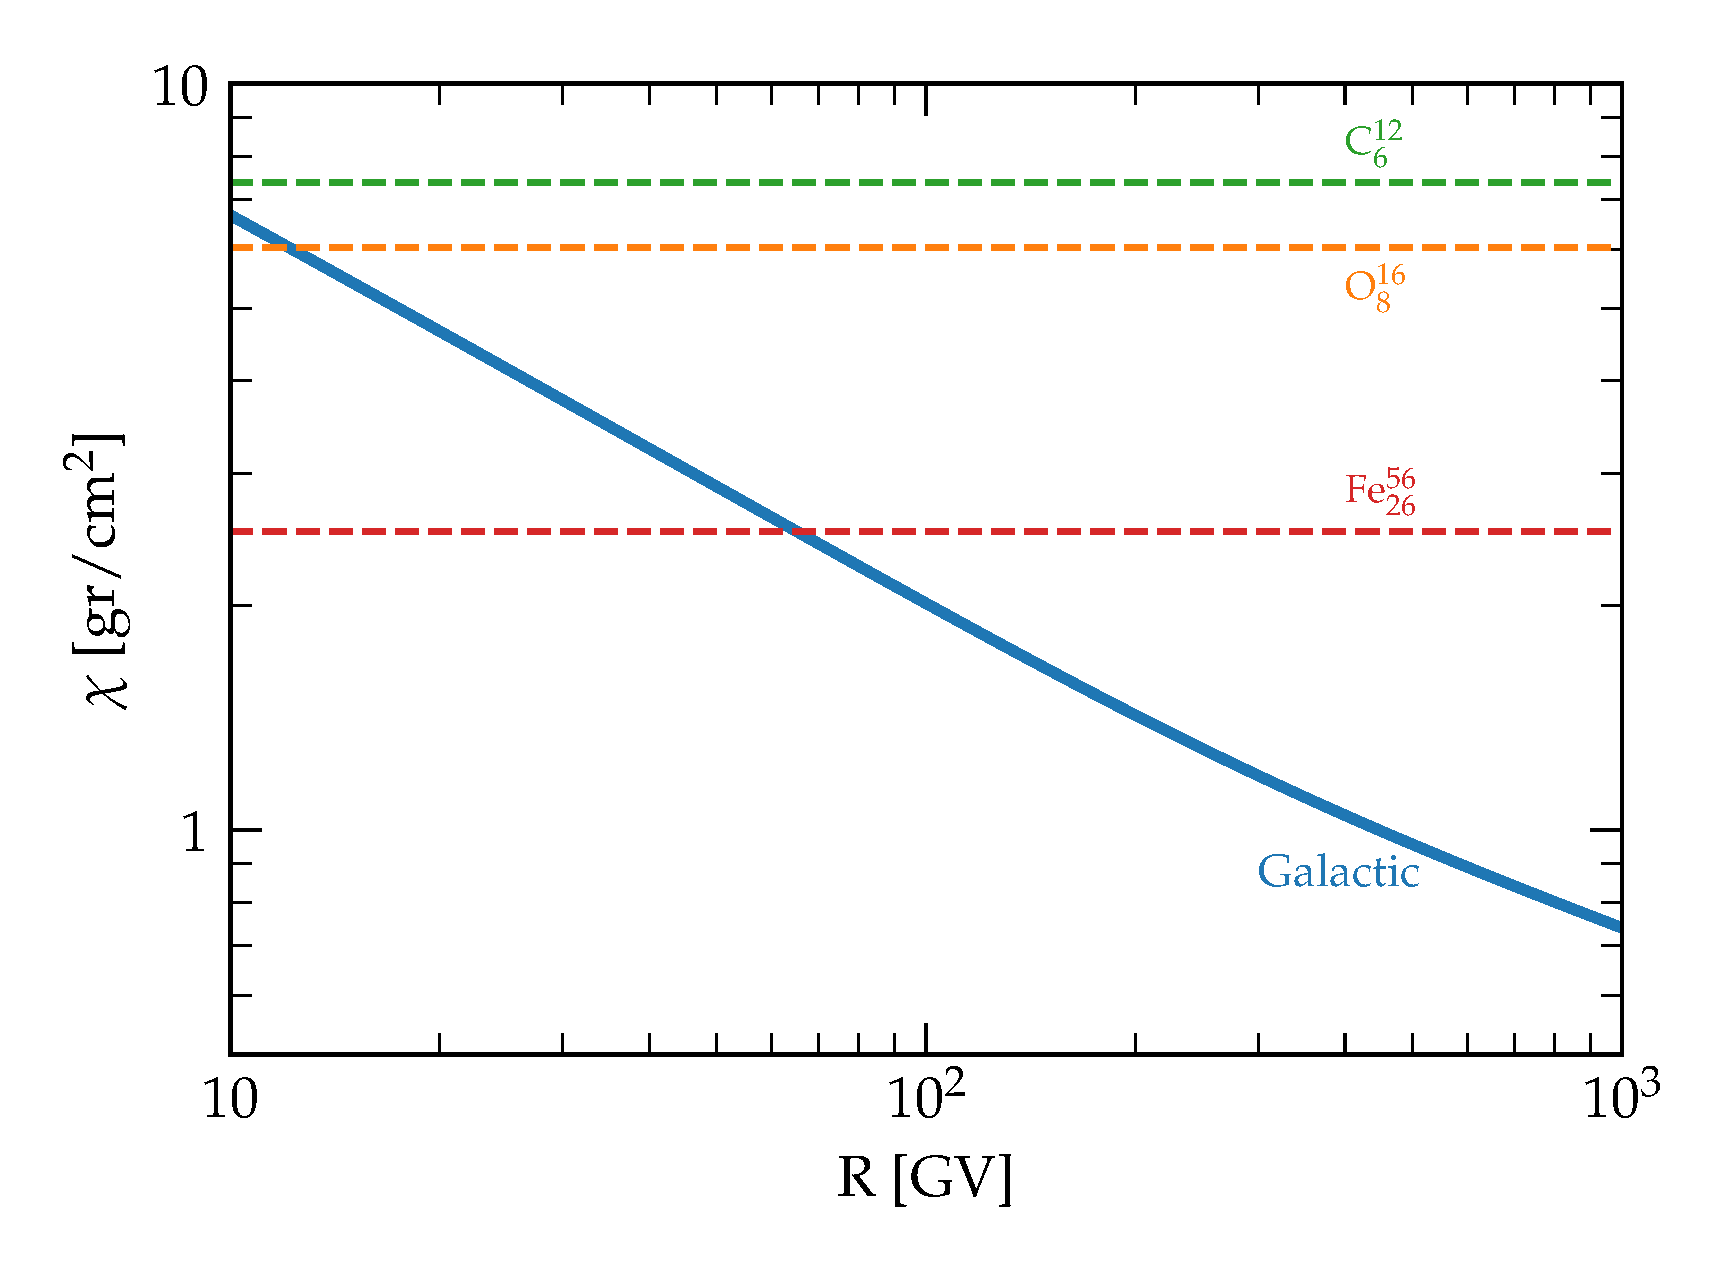
\includegraphics[width=0.6\textwidth]{figures/grammage_critical.pdf}
\caption{The grammage corresponding to the best fit model described in~\cite{Schroer2021prd} as a function of rigidity is shown as a solid blue line. The dashed lines refers to carbon (green), oxygen (orange), and iron (red) inelastic critical grammage.}
\label{fig:grammage}
\end{figure}

Written in this form, the grammage serves to quantify the average density, $\bar n$, that particles traverse while moving across the Galaxy for a duration corresponding to the time it takes for particles to leave the Galaxy, $\tau_{\rm esc}$.

Furthermore, we define the critical grammage as 
%
\begin{equation}
\rchi_{\rm cr} = \frac{m_{\rm p}}{\sigma_\alpha} \simeq 40 \, A^{-2/3} \, \text{gr} \, \text{cm}^{-2}
\end{equation}

The critical grammage represents the threshold value where spallation becomes significant, requiring the grammage to be at least $\rchi_{\rm cr}$.

By using these definitions, the propagated spectrum of a species $\alpha$ can be expressed as:
%
\begin{equation}
f_{0,\alpha}(p) = \frac{Q_{0,\alpha}(p)}{2n_{\rm d}hm_{\rm p}c} \frac{1}{\frac{1}{\rchi(p)} + \frac{1}{\rchi_{\rm cr}}}
\label{eq:finalprimary}
\end{equation}

In the limit of strong and weak spallation, we obtain:
%
\begin{equation}
f_{0,\alpha}(p) = Q_{0,\alpha}(p) \times
\begin{cases}
\frac{1}{2n_{\rm d}hm_{\rm p}c}\rchi_{\rm cr} & \text{if } \, \rchi(p) \gg \rchi_{\rm cr} \\
\frac{H}{2D(p)} & \text{if } \, \rchi(p) \ll \rchi_{\rm cr}
\end{cases}
\end{equation}

Hence, when $\chi(p)\gg \chi_{\rm cr}$, spallation dominates, the spectrum at the disc will exhibit a similar slope to the injection spectrum. Conversely, in the limit of weak spallation, the diffusion-dominated solution is recovered, resulting in an observed spectrum that is \emph{steeper} than the source spectrum due to the momentum dependence of the diffusion coefficient.

At low energies, spallation may dominate because $D(p)$ is an increasing function of momentum, and spallation cross sections are independent of energy. For heavy nuclei, the effects become particularly relevant at higher energies due to the scaling with mass in equation~\eqref{eq:scalingcs}. In figure~\ref{fig:grammage} the critical grammage for different nuclei is compared with the Galactic value obtained by several recent analysis~\cite{Evoli2019prd,Weinrich2020aa}. For Iron, one of the heaviest species present in the Galactic radiation, the critical grammage becomes ruling for rigidities\footnote{We remind that rigidity is defined as momentum over charge, $p/Z$.} below $\lesssim 60$~GV~\cite{Schroer2021prd}.

Equation~\eqref{eq:finalprimary} highlights that if we could somehow measure the grammage, we would be able to retrieve the acceleration efficiency $\xi_{\rm CR}$ from the spectrum observed at Earth. This parameter is of crucial importance for the development of any acceleration paradigm.

However, obtaining this crucial information relies on a different observable, which will be discussed in detail in the next section.

\section{The secondary over primary ratio}
\label{sec:secondaryoverprimary}

As mentioned in the Introduction, light and fragile elements such as lithium, beryllium, and boron are mainly synthesized through the collisions of galactic CRs with the interstellar gas in the Galaxy. Here we investigate the production of these elements, and how they constrain CR models for Galactic propagation. 
%
For the sake of simplicity, we focus on a case with only carbon as the primary species ($\alpha' = \text{C}$), whereas boron is almost exclusively created in secondary processes ($\alpha = \text{B}$).

The solution for carbon has been obtained in the previous section and is given by:
%
\begin{equation}
f_{0,\rm C}(p) = \frac{Q_{0,\rm C}}{2n_{\rm d}h m_{\rm p}c} \frac{1}{\frac{1}{\rchi_{\rm C}(p)} + \frac{1}{\rchi_{\rm cr, C}}}
\end{equation}

Since boron is a pure secondary species, the solution of its transport equation takes the same form as the previous equation, with the injection rate proportional to the equilibrium solution for carbon:
%
\begin{equation}
4 \pi Q_{\rm B}(p) p^2 dp = 2 h n_{\rm d} c \sigma_{\rm C \rightarrow B} 4 \pi \delta(z) f_{\rm C}(p^\prime) p^{\prime \, 2} dp^\prime
\end{equation}

Here, $A$ is the atomic number of carbon, and the Jacobian $\frac{dp'}{dp} = \frac{A}{A-1}$ is introduced to ensure conservation of energy per nucleon.

The spectrum of boron in the disc is then given by:
%
\begin{equation}
f_{0,\rm B}(p) 
%= \frac{Q_{0, \rm B}(p)}{2 n_{\rm d} h m_{\rm p} c} \frac{1}{\frac{1}{\rchi_{\rm B}(p)} + \frac{1}{\rchi_{\rm cr, B}}}
= \frac{\sigma_{\rm C \rightarrow B}}{m_{\rm p}}  \frac{1}{\frac{1}{\rchi_{\rm B}(p)} + \frac{1}{\rchi_{\rm cr, B}}} f_{0, \rm C}\left(\frac{A}{A-1}p\right) \left(\frac{A}{A-1} \right)^3
\end{equation}

This leads to the B/C ratio as:
%
\begin{equation}
\frac{\rm B}{\rm C} \simeq \frac{1}{\rchi_{\rm cr, C\rightarrow B}} \left(\frac{1}{\rchi(p)} + \frac{1}{\rchi_{\rm cr, B}}\right)^{-1}
\label{eq:chibc}
\end{equation}

It is important to note that the boron-to-carbon ratio is independent of the primary source and is solely a function of the grammage and relevant cross-sections.

Once again, considering the two limits of strong and weak spallation, we find the following. 
%
In the case of strong spallation:
%
\begin{equation}
\frac{\rm B}{\rm C} \oset{\rchi \gg \rchi_{\rm cr}}{\, \longrightarrow \,} \frac{\rchi_{\rm cr, B}}{\rchi_{\rm cr, C\rightarrow B}} 
= \frac{\sigma_{\rm C \rightarrow B}}{\sigma_{\rm B}} 
\simeq 0.3
\end{equation}

This results in a constant B/C ratio as a function of energy, with the value determined solely by the cross-sections~\cite{Evoli2019prd}.

In the opposite limit:
%
\begin{equation}
\frac{\rm B}{\rm C} \oset{\rchi \ll \rchi_{\rm cr}}{\, \longrightarrow \,} \frac{\rchi(p)}{\rchi_{\rm cr, C\rightarrow B}} \propto \frac{1}{D(p)}
\label{eq:bchene}
\end{equation}

Hence, in this limit, the B/C ratio is expected to decrease with increasing energy. 
%
Moreover, by measuring the B/C ratio as a function of energy, we can estimate the energy dependence of the grammage and, consequently, of the diffusion coefficient of Galactic CRs.

It is difficult to overemphasize the significance of this result. 
%
The recent AMS-02 data on secondary-to-primary ratios (see figure~\ref{fig:bcams02}) clearly demonstrate that the B/C ratio decreases with increasing rigidity above $\sim$10 GV. %, exhibiting a scaling behavior approximately proportional to the rigidity raised to the power of $\simeq -1/3$. 
%
This indicates that we are operating in the regime of weak spallation, allowing us to infer the Galactic grammage from this observable.
%
A quick fit to data shown in figure~\ref{fig:bcams02}, using $\sigma_{\rm C \rightarrow B} \simeq 60$~mb, indicates that the grammage is of the order of $8.5$~gr cm$^{-2}$ at $\simeq 10$~GV, exhibiting a scaling behavior approximately proportional to the rigidity raised to the power of $\simeq -1/3$. 

Furthermore, by leveraging the observed slope of the proton spectrum, around 2.8 in the energy range 20-200 GeV (see figure~\ref{fig:protonshe}), we can estimate the injection slope $\gamma$ by recovering from \S\ref{sec:protons} that $\gamma + \delta \approx 2.8$, guiding us to $\gamma \approx 2.4$. 
%
Consequently, we arrived to the conclusion that the energy spectra of CRs at their sources must be relatively \emph{soft}, challenging the predictions based on the original version of DSA\footnote{Again, for a more comprehensive treatment of this topic, we refer readers to D.~Caprioli's lecture notes in this volume.}.

Note that equation~\eqref{eq:grammage} shows that by measuring the grammage, we can only determine the combination $H/D$, and therefore we cannot determine the normalization of the diffusion coefficient without the knowledge of the halo size.

\begin{figure}
\centering
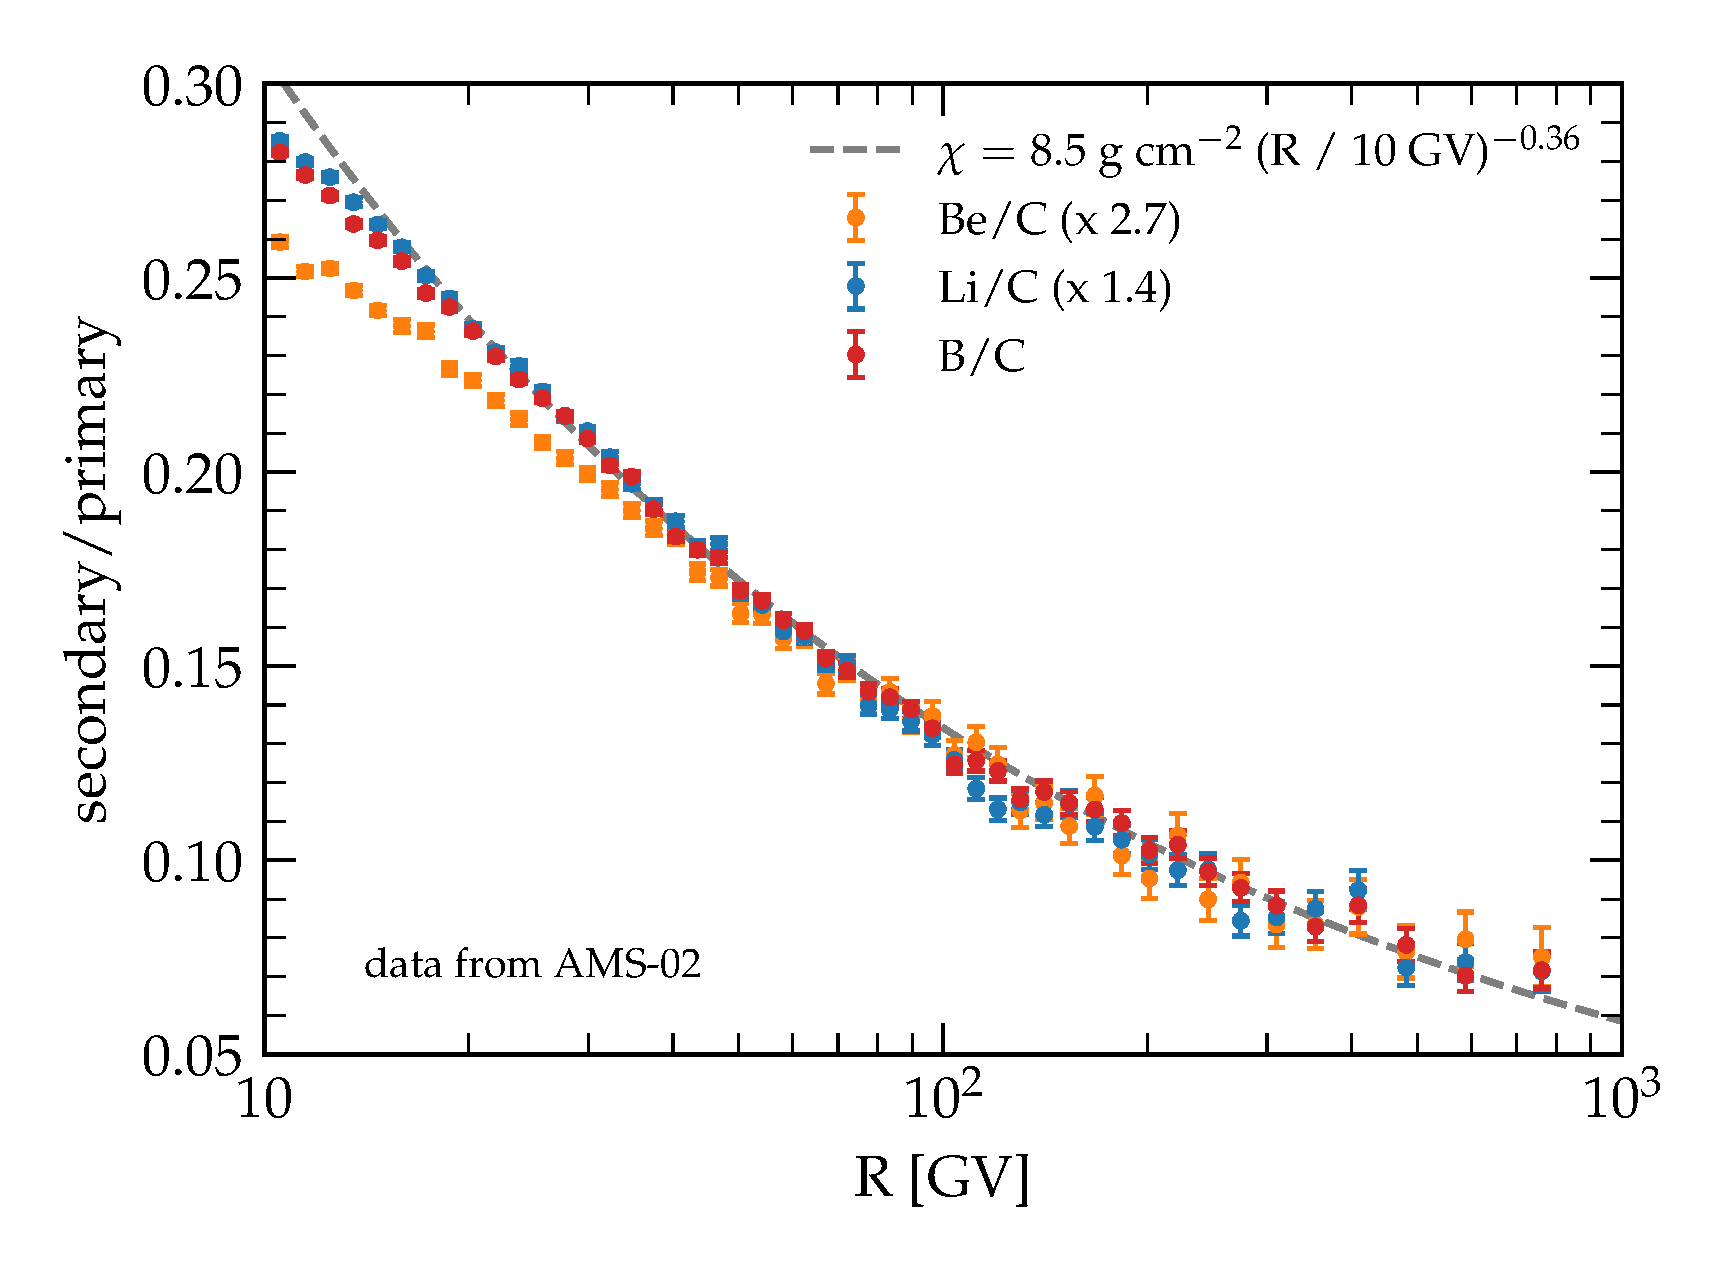
\includegraphics[width=0.6\textwidth]{figures/LiBeB_C_AMS02.pdf}
\caption{Secondary-to-primary ratios as function of rigidity measured by the AMS-02 experiment~\cite{AMS02libeb}. The power-law fit at high energies is also shown.}
\label{fig:bcams02}
\end{figure}

To access the diffusion coefficient, we can make certain assumptions about the size of the Galactic halo. 
%
In the 1960s, it was proposed that observing radio emission from our Galaxy could provide insights into the region where CRs reside~\cite{Ginzburg1961ptps}. This is because radio emission is generated through synchrotron radiation emitted by high-energy electrons. The morphology of the radio emission indicates that it extends well beyond the Galactic disc, where magnetic fields allow particle diffusion to occur.

The region where CRs are predominantly found has a scale of approximately kiloparsecs, significantly larger than the size of the Galactic disc. By utilizing the B/C ratio to estimate $H/D$ and making assumptions about $H$, we can then determine the diffusion coefficient, $D$, and subsequently calculate the average time that CRs spend within the Galaxy, given by $H^2/D$. 

At around 10 GeV, B/C amounts roughly to $\sim 0.3$, which implies\footnote{We have employed equation~\eqref{eq:grammage} in conjunction with the relationship $2h \rho_{\rm d} = \mu_{\rm d}$.} a confinement time of approximately $\sim$100~Myr for $H \sim 3$~kpc, and it decreases as the energy increases.

To delve deeper into this topic, we require a reliable method for measuring this time. In the upcoming section, we will explore how secondary unstable isotopes, which decay with a timescale comparable to the confinement time, can serve as a cosmic clock, enabling us to estimate the Galactic residence time.

Combining this information with the grammage, which yields $H/D$, will allow us to obtain the average value of the diffusion coefficient on Galactic scales.

As we will discuss in 
\S\ref{sec:implications}, these advancements will pave the way for a theoretical comprehension of the microphysics behind the scattering and diffusion of cosmic particles by the fluctuations present in the interstellar turbulent magnetic fields.

\begin{figure}
\centering
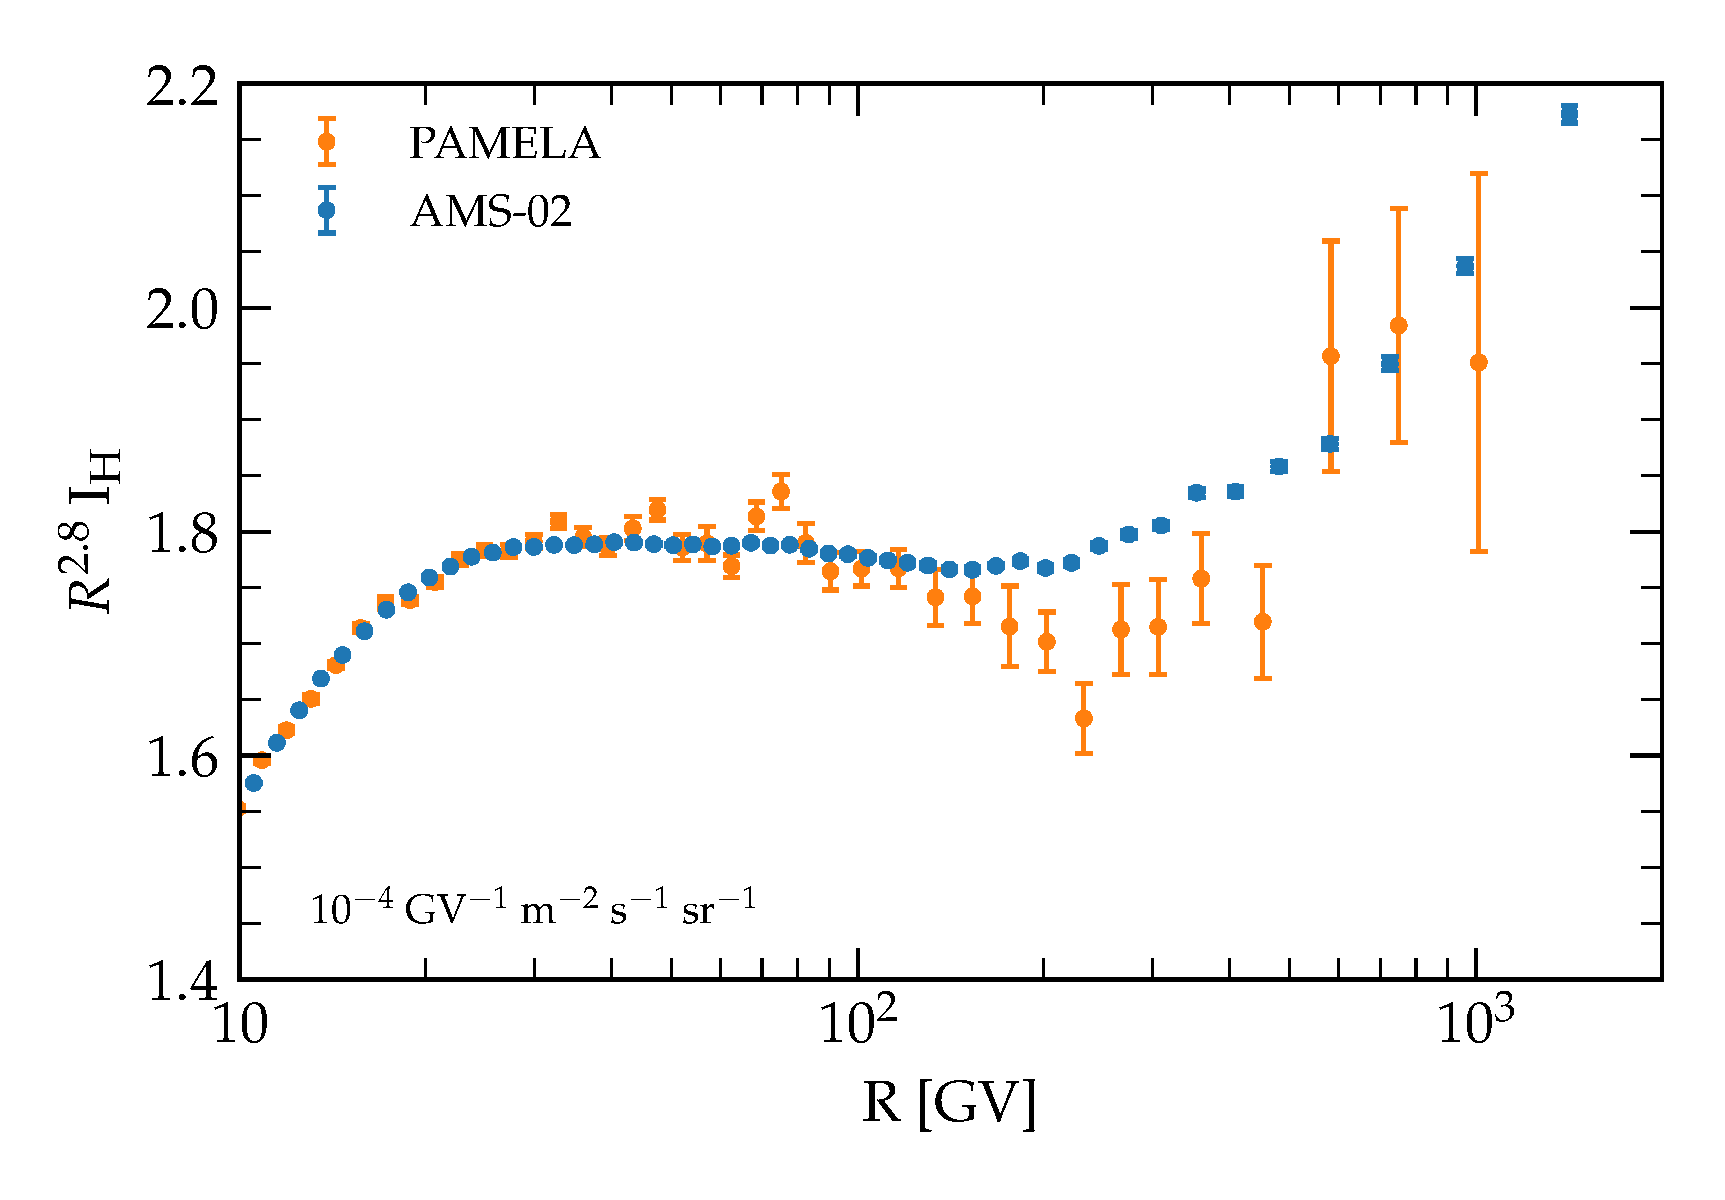
\includegraphics[width=0.6\textwidth]{figures/protons_he.pdf}
\caption{The spectrum of protons as function of rigidity, measured by the AMS-02, and PAMELA experiments~\cite{AMS02results,PAMELA.2011.proton}.}
\label{fig:protonshe}
\end{figure}

The scrupulous reader may have noticed in figure~\ref{fig:protonshe} that the canonical slope, approximately $\sim 2.8$, does not extend up to very high energies. Instead, the CR spectrum exhibits a notable change of slope, commonly referred to as a \emph{break}, at an energy around $200$~GeV, where it hardens to about $\sim 2.6$.
%
At these energies, however, the equilibrium spectrum must be determined by the ratio $Q(p)/D(p)$, where both quantities are assumed to follow a pure power-law behavior. 

Prior to questioning well-established theoretical models to seek the elusive physical mechanism responsible for this bizarreness, it is crucial to ascertain whether the break should be attributed to the numerator or the denominator of equation~\eqref{eq:finalprimary}. 
%
In other words, we need to identify whether the break occurs at the injection stage or during the transport of CRs in the Galaxy.

Equation~\eqref{eq:bchene} quickly unravels this conundrum! 

Specifically, being dependent only on grammage, the secondary-over-primary ratio is the key parameter to examine. 
%
If the same change of slope is also present in the B/C ratio, then the conclusion must be that it is due to propagation, indicating a break in the diffusion coefficient. On the other hand, if no such change of slope is observed in the B/C ratio, then we must look for the solution at the injection stage.

\begin{figure}
\centering
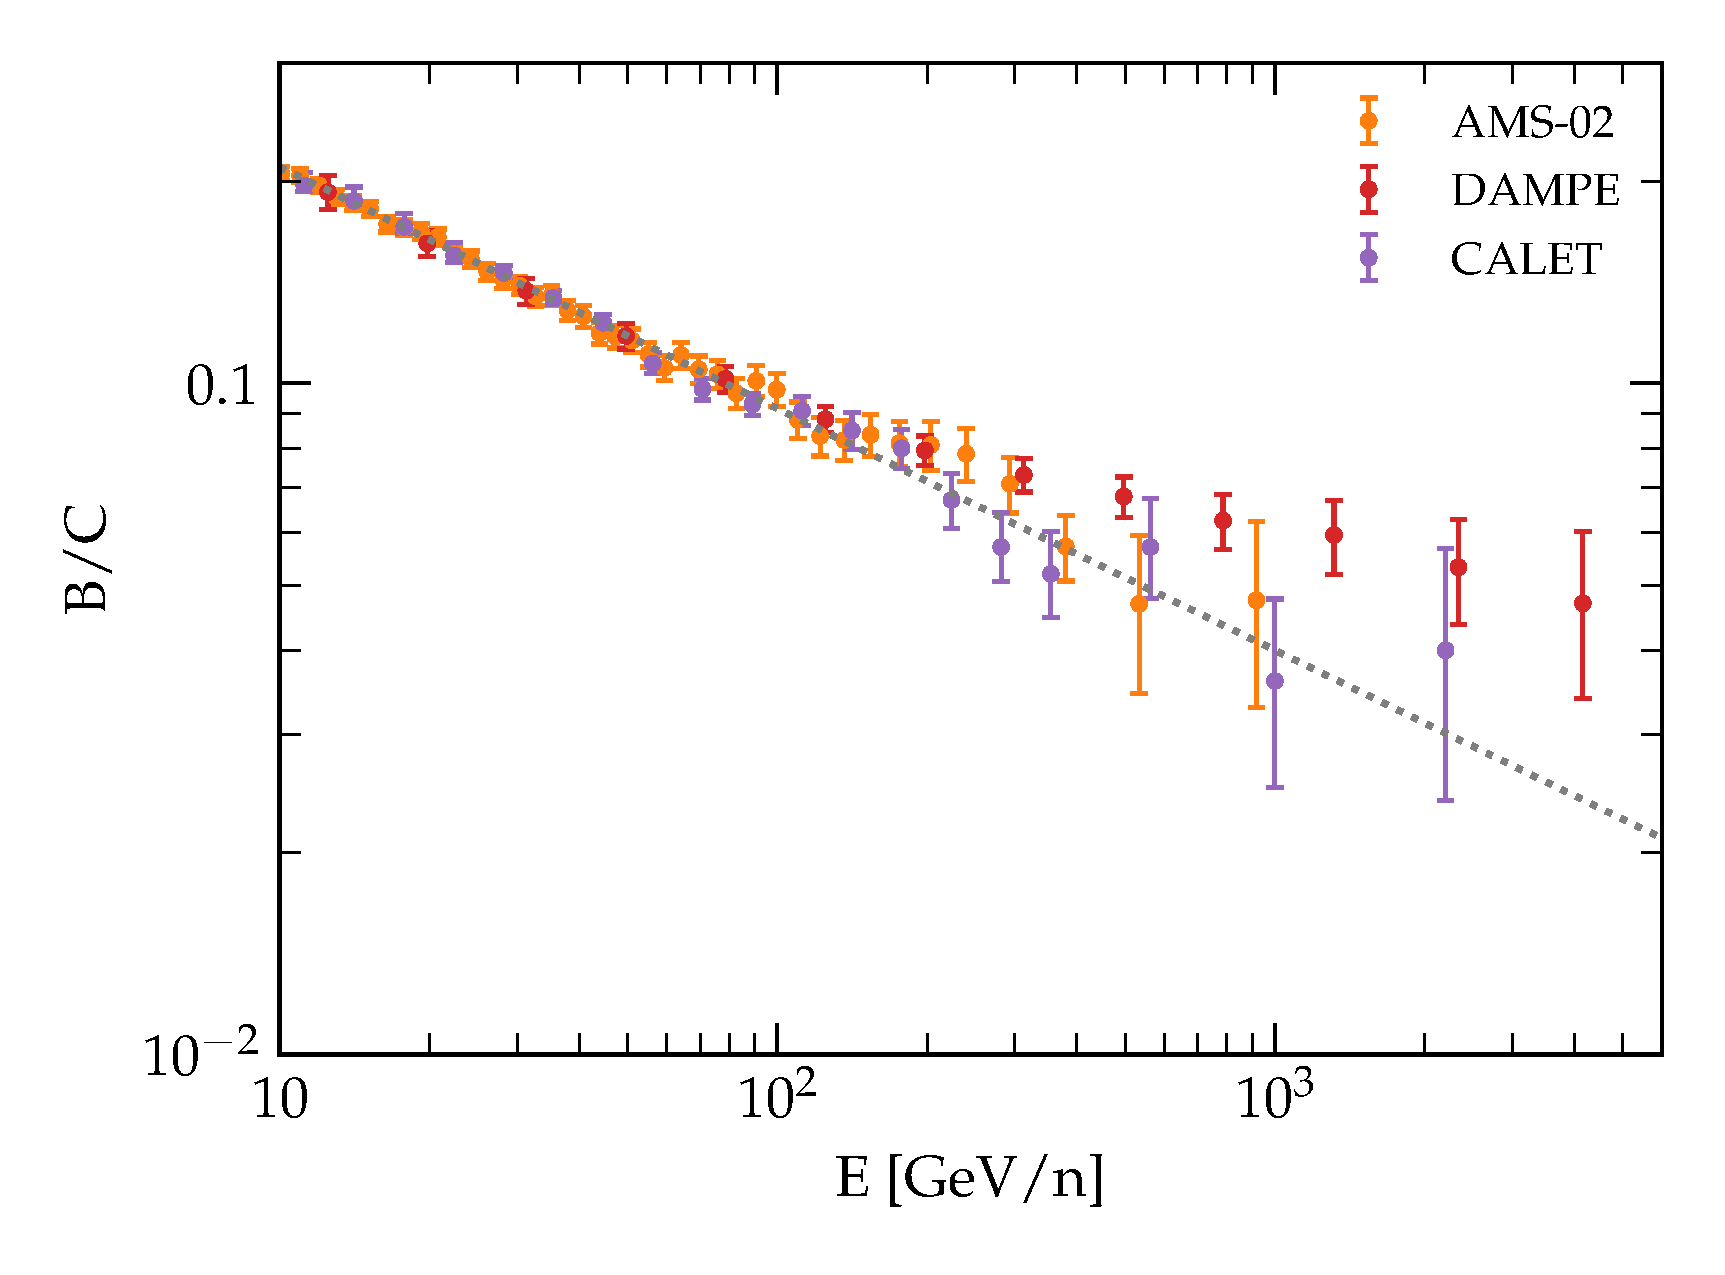
\includegraphics[width=0.6\textwidth]{figures/BC_highenergy.pdf}
\caption{Boron-to-carbon ratio as function of kinetic energy per nucleon measured by the AMS-02~\cite{AMS02results}, CALET~\cite{CALET.2022.BC} and DAMPE~\cite{DAMPE.2022.BC} experiments.}
\label{fig:bchighen}
\end{figure}

As shown in figure~\ref{fig:bchighen}, where we extend B/C data over the multi-TeV range thanks to measurements by DAMPE and CALET, the situation indeed aligns with the former scenario, and thereby all the current explanations of this feature are given in terms of some alteration in the galactic transport. 
%
These revisions in the transport of CRs might be associated with a spatial dependence of the diffusion coefficient, as proposed in ~\cite{Tomassetti2012apj}, or due to the transition from selfgenerated turbulence to preexisting turbulence, see, e.g.,~\cite{Evoli2018prl}.

At such, the recently reported departures from an otherwise boring scale-free power-law behavior in the galactic CR spectra are of paramount importance, as they offer valuable insights into the fundamental mechanisms governing the propagation of CRs in magnetized environments.

%%%%%%%%%% SECTION %%%%%%%%%%
\section{Unstable nuclei: the case of beryllium}
\label{sec:unstable}

The average time that CRs spend in the Galaxy before escaping can be determined by studying the suppression of the flux of unstable nuclei due to radioactive decay. By comparing the fluxes of two isotopes of the same chemical element—one stable and the other unstable—it is possible to measure this suppression and estimate $\tau_{\rm esc}$.

Beryllium is an element that is very rare in ordinary matter, and the majority of beryllium nuclei in CRs are secondary particles formed through the fragmentation of heavier nuclei. 
%
It has two stable isotopes, $^9$Be and $^7$Be (if fully ionized), as well as one $\beta^-$ unstable isotope, $^{10}$Be, with a half-life of $\tau_{1/2} = (1.386 \pm 0.016)$ Myr~\cite{Chmeleff2010nimb}. 
%
The decay of $^{10}$Be mainly produces $^{10}$B, thus altering the abundance of this stable element.

The transport equation for $^{10}$Be can be treated as that of a secondary species, assuming (for simplicity) only one parent nucleus. 
%
Additionally, a term describing decay in the Galaxy reference frame is included:
%
\begin{equation}
-\frac{\partial}{\partial z} \left[ D_{\rm Be} \frac{\partial f_{\rm Be}}{\partial z} \right] =
- \frac{f_{\rm Be}}{\tau_{\rm f, Be}} 
- \frac{f_{\rm Be}}{\gamma \tau_{\rm d, Be}} 
+ \frac{f_{\rm C}}{\tau_{\rm f, C \rightarrow Be}} 
\end{equation}
%
Here, $\tau_{\rm d} = \tau_{1/2} / \ln(2)$ represents the rest-frame lifetime of $^{10}$Be, and $\gamma$ accounts for time dilation effects.
%
At sufficiently high energies, $^{10}$Be decays on a timescale longer than $\tau_{\rm esc}$, effectively behaving as a stable isotope.

It is worth emphasizing that this is the first case we have discussed where the source or loss term in the transport equation does not exhibit a $\delta$-function shape in $z$. This distinction arises due to the inclusion of the decay term, which introduces a new complexity that necessitates a dedicated approach for solving the corresponding transport equation.

Outside the disk $z \neq 0$, the transport equation becomes:
%
\begin{equation}
-\frac{\partial}{\partial z} \left[ D_{\rm Be} \frac{\partial f_{\rm Be}(z)}{\partial z} \right] + \frac{f_{\rm Be}(z)}{\gamma\tau_{\rm d, Be}} = 0
\end{equation}

Unlike the case of stable elements, the diffusive flux is not conserved. 
%
To find a solution, we assume the form:
%
\begin{equation}
f(z) = A {\rm e}^{-\alpha z} + B {\rm e}^{\alpha z}
\end{equation}
%
which implies $\alpha^{-1} = \sqrt{D \gamma\tau_{\rm d}}$, where we have assumed that the diffusion coefficient is spatially constant.

By imposing the appropriate boundary conditions, we obtain (introducing $y \equiv {\rm e}^{\alpha H}$):
%
\begin{equation}
\frac{f_{\rm Be}(z)}{f_{\rm Be,0}} =  -\frac{y^2}{1 - y^2} {\rm e}^{-\alpha z} + \frac{1}{1- y^2} {\rm e}^{\alpha z} 
\label{eq:bespatial}
\end{equation}

The value of the distribution function at $z=0$ can be obtained by integrating above and below the disk:
%
\begin{equation}
\left. -2 D_{\rm Be} \frac{\partial f_{\rm Be}(T)}{\partial z} \right|_{0^+} =
- 2 h n_{\rm d} c \sigma_{\rm Be} f_{0, \rm Be}
+ 2 h n_{\rm d} c \sigma_{\rm C \rightarrow Be} f_{0, \rm C} 
\end{equation}

To obtain the flux, we utilize equation~\eqref{eq:bespatial}, yielding:
%
\begin{equation}
\left. \frac{\partial f_{\rm Be}(T)}{\partial z} \right|_{0^+} = \alpha \frac{1+y^2}{1-y^2} \, f_{\rm Be,0}
\end{equation}

Combining these equations, we arrive at:
%
\begin{equation}
f_{\rm Be,0}(p) \left[  \frac{\sigma_{\rm Be}}{m_{\rm p}} - \frac{1}{c m_{\rm p} h n_{\rm d}} \sqrt{\frac{D_{\rm Be}(p)}{\gamma \tau_{\rm d, Be}}} \frac{1+y^2}{1-y^2} \right] = 
\frac{\sigma_{\rm C\rightarrow Be}}{m_{\rm p}} f_{\rm C,0}(p)
\end{equation}

Alternatively, one can write it in terms of grammages
%
\begin{equation}
\frac{f_{\rm Be,0}}{f_{\rm C,0}}(p) = 
\frac{1}{\rchi_{\rm cr, C \rightarrow Be}}  \left[  \frac{1}{\rchi_{\rm cr, Be}} + \frac{1}{\rchi_{\rm Be}^\prime(p)} \right]^{-1}  
\end{equation}
%
where $\rchi^\prime$ represents the grammage modified by the decay term and can be expressed as:
%
\begin{equation}
\rchi^\prime_{\rm Be}(p) = \rchi_{\rm Be}(p) \frac{1}{\alpha H} \frac{y^2 - 1}{y^2 + 1} 
\end{equation}

We observe that at high energies, when the proper decay time becomes much larger than the confinement time ($\gamma \tau_{\rm d} \gg \frac{H^2}{D}$), we have $\alpha H \rightarrow 0$ and expanding in Taylor series:
%
\begin{equation} 
\rchi_{\rm Be}^\prime(p) 
\oset{\gamma\tau_{\rm d} \gg \tau_{\rm esc}}{\longrightarrow} 
\rchi_{\rm Be}(p)
\end{equation}

\begin{figure}
\centering
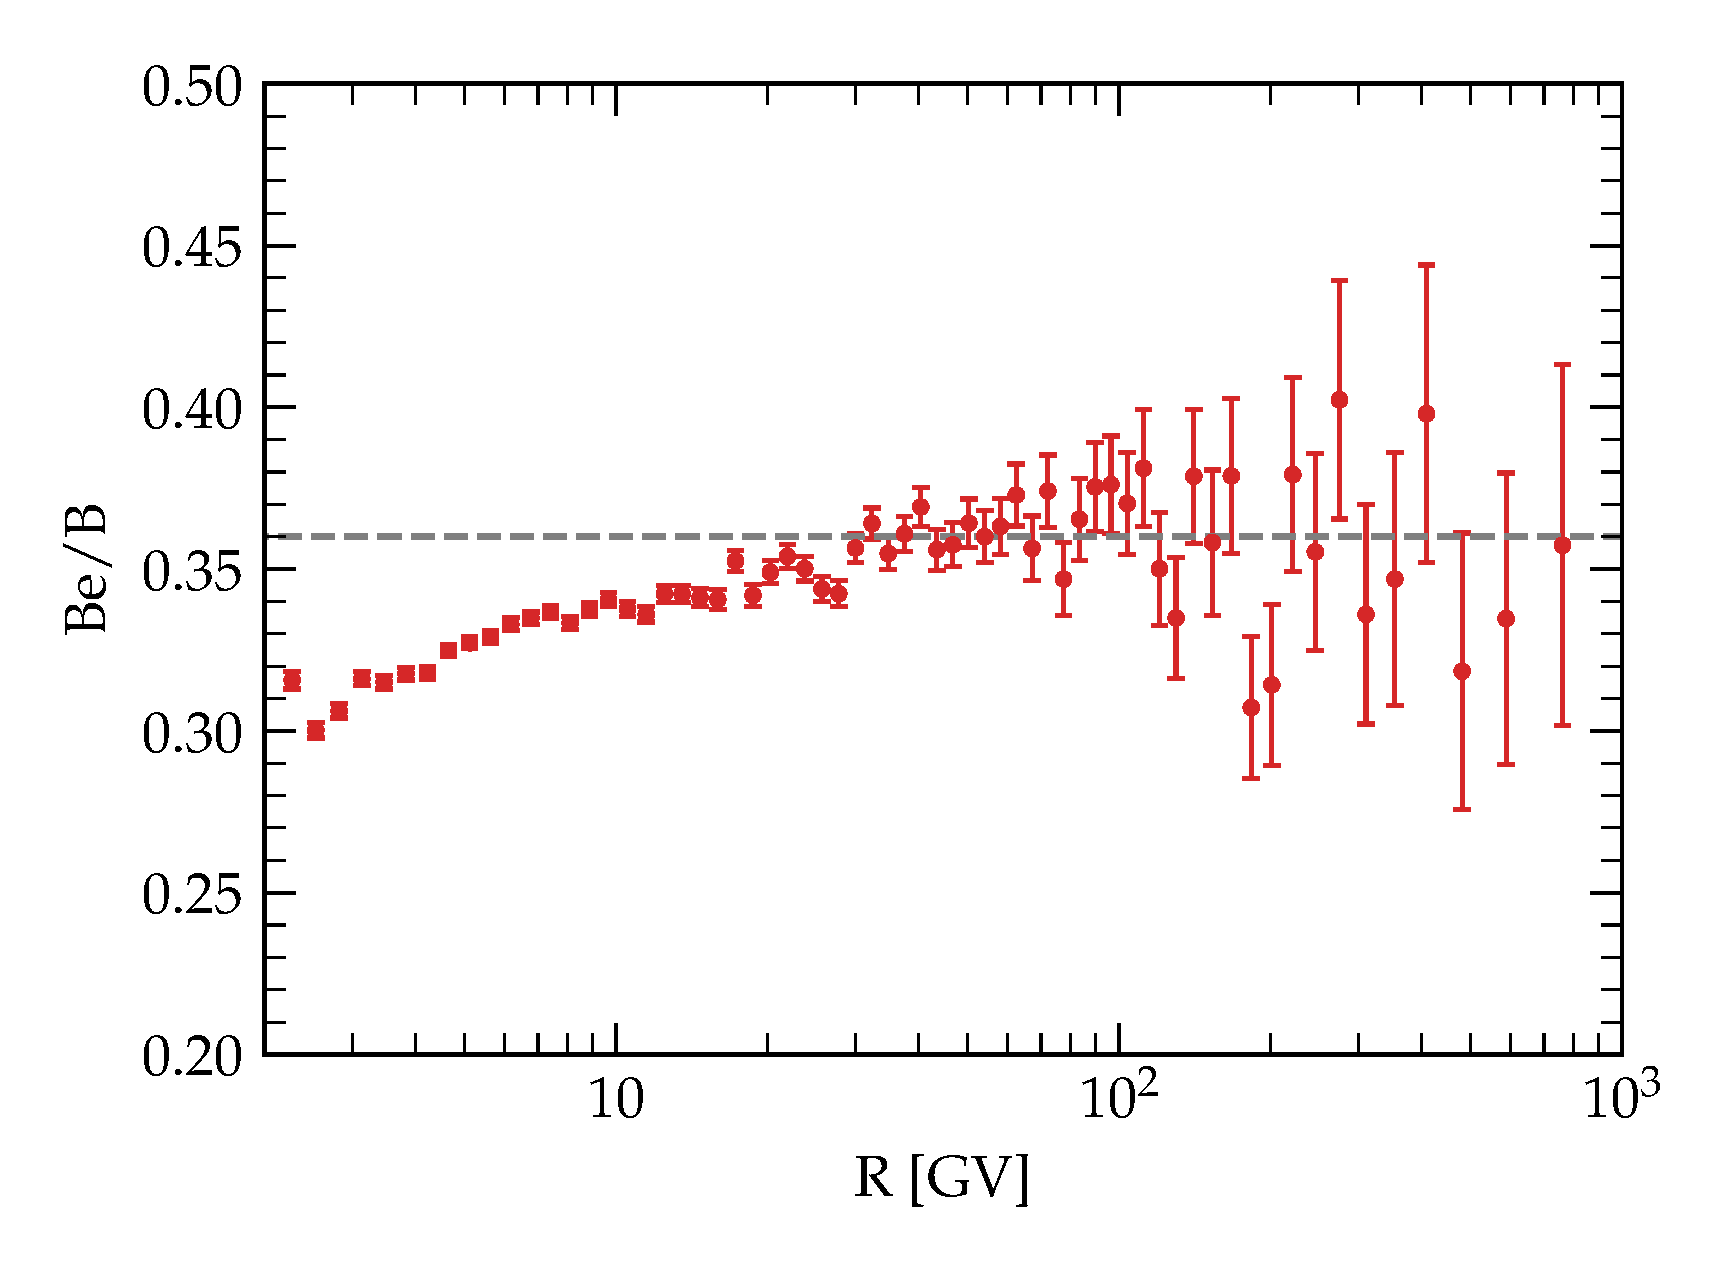
\includegraphics[width=0.6\textwidth]{figures/BeB_AMS02.pdf}
\caption{Ratio of Beryllium over Boron fluxes as measured by AMS-02~\cite{AMS02libeb}. The dotted line shows the case without decay for 10Be.}
\label{fig:beb}
\end{figure}

As expected $\tau_{\rm d}$ cancels out from the grammage, and we recover in this limit the solution obtained for a stable element.

In the opposite limit, $y \rightarrow \infty$, and the modified grammage $\rchi_{\rm Be}^\prime(p)$ approaches a simplified form:
%
\begin{equation}
\rchi_{\rm Be}^\prime(p) 
\oset{\gamma\tau_{\rm d} \ll \tau_{\rm esc}}{\longrightarrow} 
m_{\rm p} n_{\rm d} h c \sqrt{\frac{\gamma\tau_{\rm d, Be}}{D_{\rm Be}(p)}} = 
m_{\rm p} \bar n c \sqrt{\gamma \tau_{\rm d} \tau_{\rm esc}} 
\label{eq:be10be9}
\end{equation}

It is important to note that in this case, it becomes crucial to account for the additional contribution to boron production arising from the decay of beryllium. This contribution can be analytically calculated using the distribution of parent beryllium in the halo, as outlined in equation~\eqref{eq:bespatial} (a detailed derivation of this contribution is provided in~\cite{Evoli2020prd}).

In the given context, the ratio of $^{10}$Be to $^9$Be fluxes can be approximated using equation~\eqref{eq:be10be9}, which relates it to the grammage ratio:
%
\begin{equation}
\frac{\rm {^{10}}Be}{\rm {^{9}}Be} \simeq \frac{\rchi^\prime_{\rm Be}}{\rchi_{\rm Be}} = \sqrt{\frac{\gamma \tau_d}{\tau_{\rm esc}}}
\label{eq:chibe10be9}
\end{equation}

The preliminary results from the AMS-02 experiment indicate a value of $\frac{\rm {^{10}}Be}{\rm {^{9}}Be} \sim 0.3$ at a kinetic energy per nucleon $T \sim 10$ GeV/n. Inverting the equation, we can estimate the escape time as $\tau_{\rm esc} \simeq 200$~Myr.

Furthermore, the relationship between the scale height $H$ and the escape time $\tau_{\rm esc}$ can be quantitatively expressed as:
%
\begin{equation}
H \sim 7 \, \text{kpc} \left(\frac{\tau_{\rm esc}}{200 \, \text{Myr}}\right) \left(\frac{\rchi}{10 \, \text{g cm}^2}\right)^{-1}
\end{equation}
%
roughly confirming the scaling estimated with the synchrotron emission.

While directly measuring the CR confinement time $\tau$ by comparing the flux of $^{10}$Be to that of $^9$Be remains challenging due to the difficulty of separating in mass the two isotopes, the AMS-02 experiment provides access to the total flux of beryllium, encompassing $^7$Be, $^9$Be, and $^{10}$Be, as well as the total flux of boron.
%
Examining the ratio of Be/B still allows us to obtain valuable information, considering that this ratio is influenced by the decay of $^{10}$Be, affecting both the numerator and the denominator (see figure~\ref{fig:beb}).

The observed behavior of the Be/B ratio at rigidities $\lesssim 30$ GV, where the ratio changes due to the decay of $^{10}$Be and not solely based on the production cross-section ratio, suggests that the escape timescale is not significantly faster than the decay timescale at that energy.

A dedicated analysis of this process, as reported in~\cite{Evoli2020prd,Weinrich2020aab,Maurin2022aa}, indicates that $H$ is approximately 6 kpc, although the possibility of a larger value cannot be excluded.

%%%%%%%%%% SECTION %%%%%%%%%%
\section{Electrons and positrons}
\label{sec:leptons}

The fraction of leptons (electrons + positrons) in the total CR flux may be small, but their unique properties make them crucial for studying fundamental astrophysical problems, such as CR propagation and the search for sources of antimatter in the Universe.

Theoretical considerations suggest that CR electrons consist of a primary component, accelerated possibly by SuperNova Remnants (SNRs) along with nuclei, and a secondary component originating from inelastic collisions between CR nuclei (mostly protons and helium) and the ISM. However, this secondary contribution accounts for only a small fraction (less than 4\%) of the total electron flux~\cite{Moskalenko1998apj,Delahaye2010aa,Evoli2021prd}.

In the standard model of CR origin, positrons were considered to be predominantly of secondary production, with a spectrum steeper than that of both primary protons and secondary nuclei (like boron) due to radiative losses. Within this framework, the positron fraction, defined as the ratio of positron flux to the sum of electrons and positrons, was expected to decrease with increasing energy. Early measurements of the positron fraction provided preliminary and intriguing evidence for a flat or even increasing trend, contradicting the standard CR transport scenario. However, the statistical limitations of these early measurements, attributed to the very low positron flux in cosmic radiation, prevented robust conclusions. Nonetheless, this finding received strong confirmation from the PAMELA experiment, which demonstrated a growing positron fraction with energy, at least up to approximately 100 GeV~\cite{PAMELA.2009.posfraction}. The excess was also observed by Fermi-LAT, which utilized Earth's magnetic field to distinguish between electrons and positrons~\cite{FERMI.2012.posfraction}. 
%
Subsequently, the positron excess was further confirmed and measured with higher accuracy at even higher energies by the AMS-02 experiment aboard the International Space Station. Thanks to its extended energy range, the AMS-02 experiment reported the first experimental observation of the positron fraction reaching a maximum around $\sim$500 GeV, followed by a sharp drop at higher energies~\cite{AMS02.2013.posfraction}.

In addition, the unambiguous measurement of electron and positron spectra separately revealed that the rise in the positron fraction is due to an excess of positrons rather than a deficit of electrons~\cite{AMS02.2019.electrons}.

These discoveries have unveiled a new population of sources that are primarily responsible for the production of electron-positron pairs. Among the various possibilities, galactic pulsars emerge as the most likely candidates for these leptonic sources, representing a remarkable breakthrough in our comprehension of the acceleration mechanisms occurring in these objects~\cite{Harding1987icrc,Aharonian1995aa,Grasso2009aph,Hooper2009jcap,Delahaye2010aa,Manconi2020prd,Amato2020arxiv}.

The propagation of electrons in the Galaxy is different from that of nuclei. At high energies, radiative losses become a dominant process, as loss-time scales proportionally to $E^{-1}$. Consequently, high-energy electrons have limited lifetimes and can only propagate within a restricted distance range.

For these high-energy electrons, the primary energy loss mechanisms are synchrotron radiation resulting from interactions with interstellar magnetic fields and inverse Compton scattering (ICS) with Galactic radiation fields (such as the cosmic microwave background, infrared, optical, and UV photons).

In the Thompson approximation, neglecting Klein-Nishina corrections to the $\gamma$-e$^-$ cross-section\footnote{In the context of the Galaxy, this assumption encounters some limitations, particularly concerning the ICS of electrons with optical and UV photons. A more accurate approach to ICS reveals spectral features arising from the diminishing Klein-Nishina cross-section of electrons as their energy surpasses around $\sim 40$~GeV when interacting with UV photons~\cite{Agaronyan1985ap,vanderwalt1991mnras,Evoli2020prl}.}, the rate of energy loss can be expressed as follows (see P.D.~Serpico's lecture notes in this volume):
%
\begin{equation}
\left| \frac{dE}{dt} \right| = \frac{4}{3} \sigma_{\rm T} c \gamma^2 \beta^2 (\mathcal U_\gamma + \mathcal U_{\rm B}) = b_0 \left( \frac{E}{10~\rm GeV} \right)^2
\end{equation}
%
Here, $\sigma_{\rm T}$ represents the Thomson cross section, $\mathcal U_\gamma$ denotes the energy density in background photons, and $\mathcal U_{\rm B} = \frac{B^2}{8\pi}$ represents the magnetic field energy density.

In Galactic environments, the energy densities $\mathcal U_i$ typically range from $\mathcal O(0.1-1~\text{eV/cm}^3)$, leading to a value of $b_0$:
%
\begin{equation}
b_0 \sim  10^{-14} \left(\frac{\mathcal U_\gamma + \mathcal U_{\rm B}}{\rm eV/cm^3}\right) \left(\frac{E}{10~\rm GeV}\right)^2 \, \text{GeV} \, \text{s}^{-1}
\end{equation}

The energy loss time turns out to be a \emph{decreasing} function with energy:
%
\begin{equation}
\tau_{\rm loss} \simeq \frac{E}{-dE/dt} \sim 30 \, \text{Myr} \left(\frac{E}{10~\rm GeV}\right)^{-1}
\end{equation}

\begin{figure}[t]
\centering
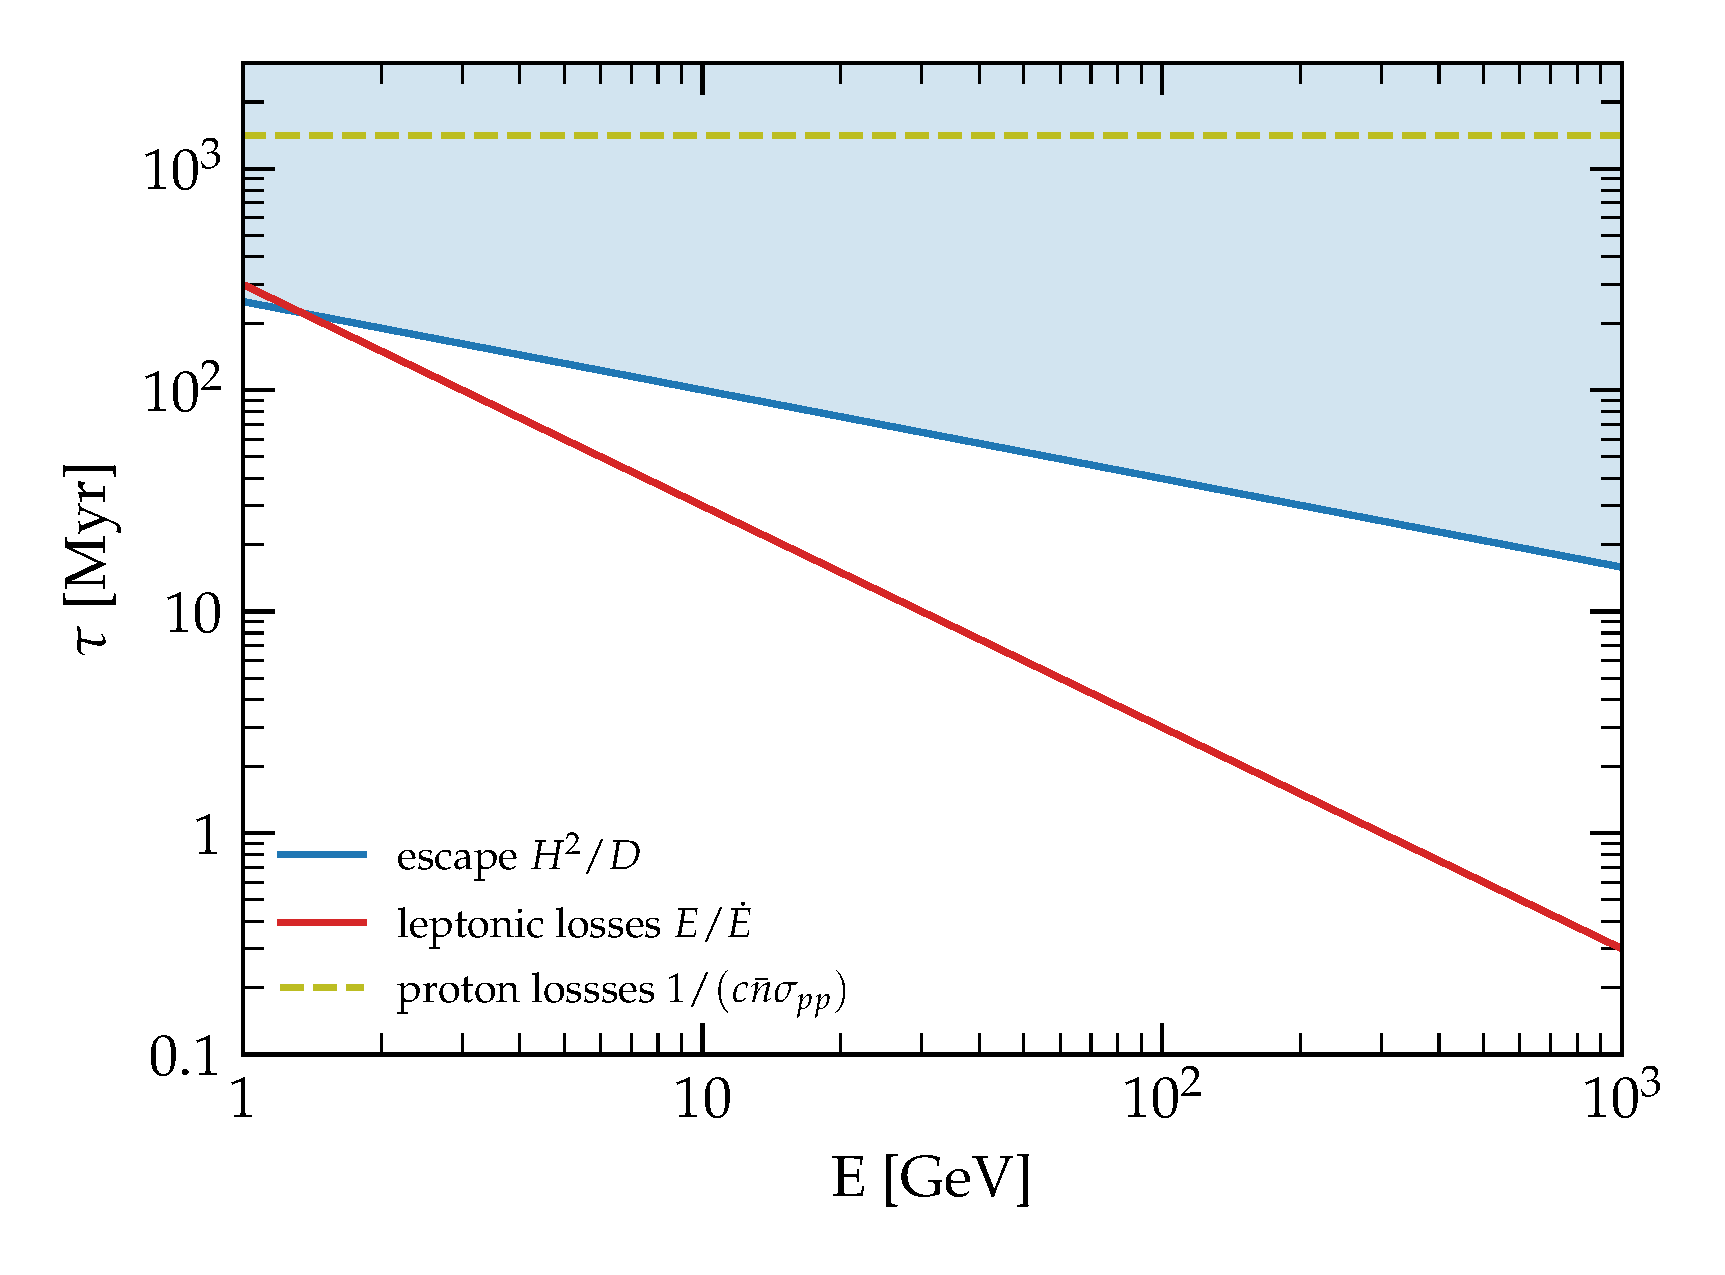
\includegraphics[width=0.6\textwidth]{figures/electron_losses.pdf}
\caption{The escape timescale derived in \S\ref{sec:protons} is confronted with energy loss timescales for protons (inelastic scattering) and leptons (synchrotron + IC) in the Milky Way.}
\label{fig:electronlosses}
\end{figure}

Figure~\ref{fig:electronlosses} provides a comparison between the energy loss timescale for electrons and the CR escape timescale as derived from nuclei. For typical values of CR transport in the ISM, the transition between the two regimes occurs at a few GeV. This implies that the Galaxy acts as an effective calorimeter for leptons, as they are expected to lose a significant portion of their energy during the typical escape time.

The transport equation for leptons is described by\footnote{For CR electrons $p \simeq E$}:
%
\begin{equation}
-\frac{\partial}{\partial z} \left [D \frac{\partial f_e}{\partial z} \right] 
= Q_e(E) \delta(z)
- \frac{1}{E^2} \frac{\partial}{\partial E} \left[ \dot E E^2 f_e \right] 
\end{equation}
%
where $\dot E$ represents the energy loss rate.

To simplify the loss term, it is convenient to approximate it as a catastrophic loss term~\footnote{Notice that assuming $\dot E \propto E^2$ and $f_e \propto E^{-\alpha}$ the relative difference between the two terms is $\sim\alpha$.}:
%
\begin{equation}
-\frac{\partial}{\partial z} \left [D \frac{\partial f_e(E)}{\partial z} \right] = Q_e(E) \delta(z) - \frac{f_e(E)}{\tau_{\rm loss}(E)}  
\label{eq:leptonprop}
\end{equation}
%
allowing the equation to be solved similarly to unstable nuclei, as the energy losses are effective throughout the propagation volume.

In the limit of negligible losses, the solution of equation~\eqref{eq:leptonprop} corresponds to that of a stable species. On the other hand, when losses dominate transport ($\tau_{\rm loss} \ll \tau_{\rm esc}$), the solution can be expressed as:
%
\begin{equation}f_{e,0}(E) 
= \frac{Q_{e,0}(E) \mathcal R_{\rm SN}}{2 \pi R_{\rm d}^2} \frac{\tau_{\rm loss}(E)}{\sqrt{D(E)\tau_{\rm loss}(E)}}
\propto E^{{-\gamma}-\frac{1 + \delta}{2}}
\label{eq:leptonsolution}
\end{equation}

\begin{figure}[t]
\centering
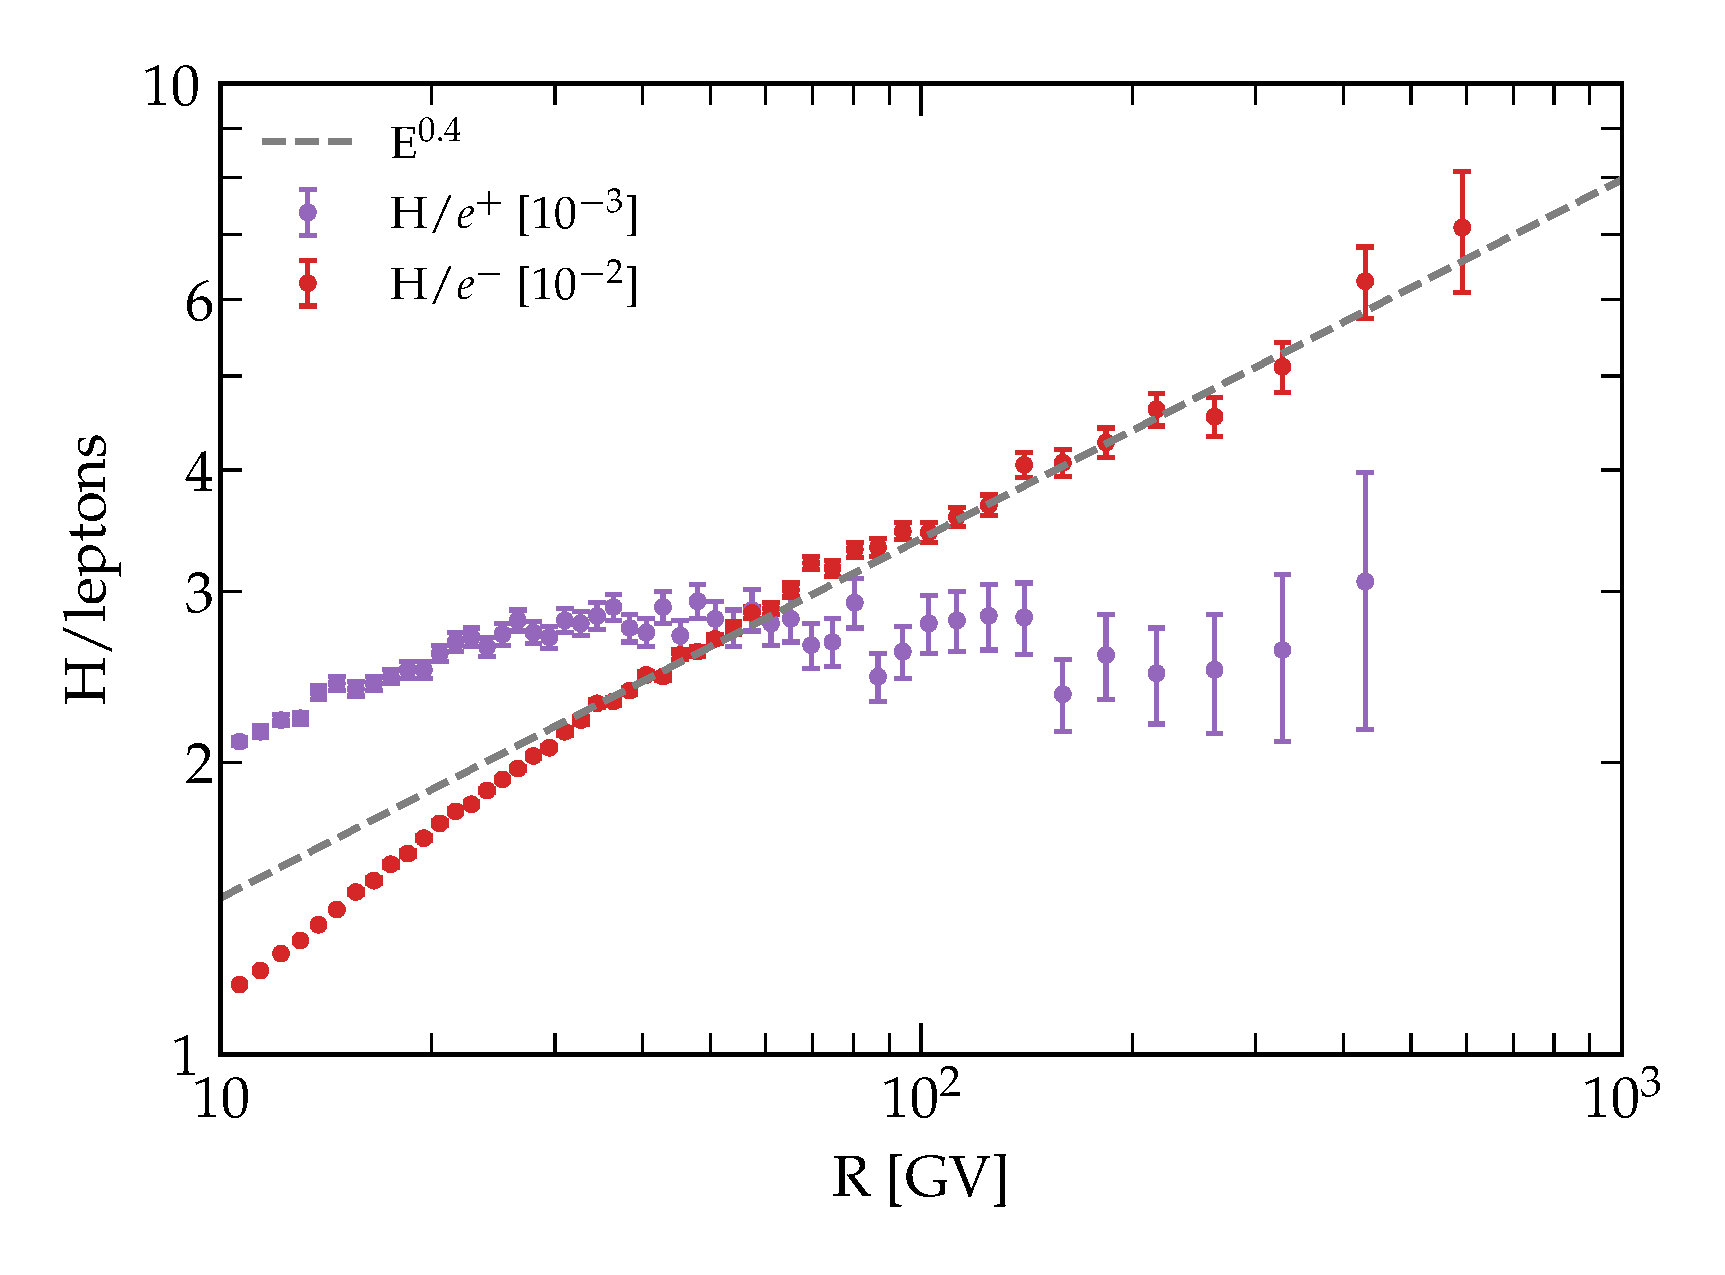
\includegraphics[width=0.6\textwidth]{figures/H_electron_ratio.pdf}
\caption{The electron(positron)-over-proton ratio as measured by AMS-02~\cite{AMS02.2019.electrons}. The high-energy power law fit is also shown as a dashed line.}
\label{fig:protonelectron}
\end{figure}

Thereby, the transition from a diffusion-dominated regime to a losses-dominated regime results in a \emph{softening} of the electron spectrum. This transition leads to a change in slope of
%
\begin{equation}
\Delta \alpha = (-\gamma-\delta) - (-\gamma-\frac{1 + \delta}{2}) = \frac{1 -\delta}{2} \simeq 0.3
\end{equation}

In Galactic CRs, the spectral break is not easily discernible due to the strong influence of solar modulation in the energy range where the break is expected to occur. 
%
Moreover, above the energy range where solar modulation plays a significant role, the most prominent feature in the electron spectrum is the spectral steepening at energies $E \lesssim$ TeV. The spectral break in the electron spectrum is well-described by a broken power-law with a change of slope of approximately $\sim$1~\cite{HESS.2008.leptons,DAMPE.2017.leptons,CALET.2018.leptons}, which is too large to be attributed to the \emph{cooling} break resulting from the transition between the diffusion-dominated and losses-dominated regimes\footnote{However, refer to~\cite{Cowsik1979apj,Lipari2017prd} for instances where unconventional approaches are explored, continuing to challenge the foundational principles outlined in these lecture notes.}. 
%
This further strengthens the evidence that electron transport is predominantly governed by energy losses throughout the entire energy range.

When comparing the proton and electron spectra, see figure~\ref{fig:protonelectron}, the difference in normalization is likely caused by the different injection mechanisms into the acceleration process for electrons and protons, as suggested by previous studies~\cite{Morlino2021mnras}.

On the other hand, we may be tempted to attribute the steeper slope of the electron spectrum solely to their energy losses.
%
Between 50 and 500 GeV, the ratio of proton flux to electron flux is well described by a power law with a slope of $\sim$0.4.

According to the prediction of the diffusion-losses model, this ratio can be expressed as:
%
\begin{equation}
\frac{f_p}{f_e} \propto \frac{E^{-\gamma_p-\delta}}{E^{{-\gamma_e}-\frac{1 + \delta}{2}}} \propto E^{-(\gamma_p-\gamma_e)} E^{\frac{1-\delta}{2}}
\end{equation}
%
where we differentiate between the injection spectra of protons ($\gamma_p$) and electrons ($\gamma_e$).

By comparing the proton-over-electron ratio with observational data, as shown in the figure, we find $\Delta \gamma = \gamma_e-\gamma_p \simeq 0.1$. This suggests that the \emph{injection} spectrum of electrons is relatively steep. More accurate analyses, accounting for realistic energy losses in the Galaxy, have found even larger values of $\Delta \gamma \simeq 0.3$~\cite{Evoli2021prd}. Resolving this issue is challenging since the most probable explanation, namely that the electron spectrum is steepened by losses in the downstream region of a SNR shock, requires extreme conditions in the late stages of SNR evolution~\cite{Cristofari2021aa}. Consequently, the origin of the steeper electron spectrum remains an open question.

Additionally, the efficiency of energy losses introduces a characteristic propagation scale, denoted as $l \simeq \sqrt{D(E) \tau_{\rm loss}}$, which serves as an effective \emph{horizon} defining the maximum distance from which an electron source of energy E can contribute to the flux observed at Earth.

Quantitatively, this scale is approximately given by
%
\begin{equation}
\frac{l}{H} \simeq \sqrt{\frac{\tau_{\rm loss}}{\tau_{\rm esc}}} \simeq 0.6 \, \left(\frac{E}{10\,\text{GeV}}\right)^{-\frac{1+\delta}{2}}
\end{equation}

Due to the existence of this horizon, only sources within a distance where the propagation time is shorter than the loss time at that energy can significantly contribute to the observed flux. Assuming a uniform distribution of sources within the Galactic disk, the estimated number of sources exploding in a loss timescale $\tau_{\rm loss}$ and lying within a distance $l$ from Earth is given by 
%
\begin{equation}\label{eq:nleptons}
N(E) \simeq \frac{\mathcal R \tau_{\rm loss} l^2(E)}{R_{\rm d}^2} \simeq 50 \left(\frac{E}{\rm TeV}\right)^{-2 + \delta}
\end{equation}

This simple estimation highlights the rapid decrease in the number of contributing sources with increasing energy, making the high-energy spectrum highly sensitive to the precise distribution of sources in our galactic vicinity.

What we learn from this is that while we routinely assume a homogeneous distribution of sources in the galactic disk, in reality, CR sources exhibit discrete spatial and temporal characteristics. As the number of sources approaches unity ($N \sim 1$), the discrete nature of the sources becomes increasingly relevant. This is in contrast to nuclei, where the spectrum is weakly dependent on the exact distribution of sources in space and time, as protons and nuclei diffuse over kiloparsec scales before escaping the CR halo, effectively averaging over the distribution of sources on these scales.

As a consequence of equation~\eqref{eq:nleptons}, it is plausible that the lepton flux in the multi-TeV energy range may receive a significant contribution from a local source. Consequently, the detection of such a source becomes an attainable goal for ongoing experiments like DAMPE and CALET, which aim to explore this energy range in the near future~\cite{Evoli2021prdb}.

\begin{figure}[t]
\centering
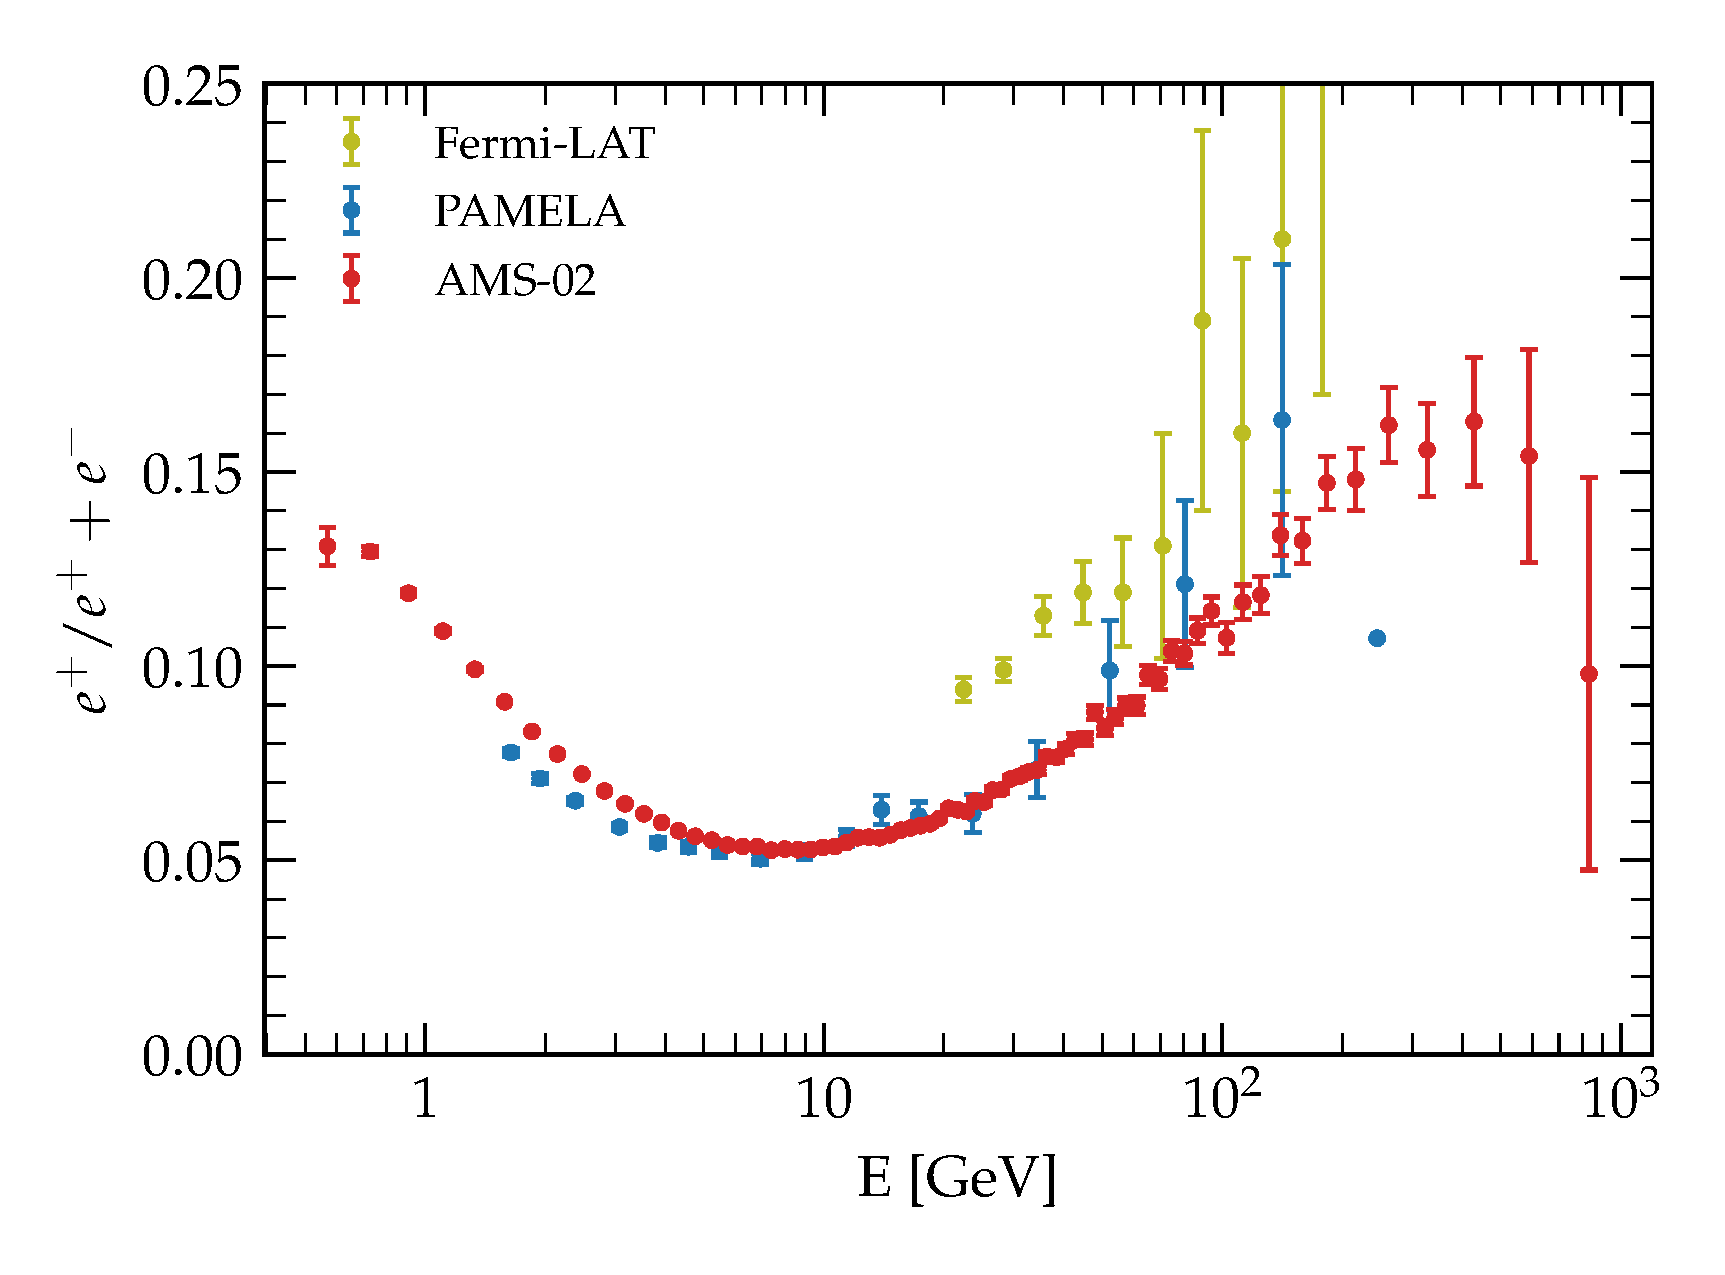
\includegraphics[width=0.6\textwidth]{figures/positron_fraction.pdf}
\caption{The positron fraction as a function of electron or positron energy as measured by PAMELA, FERMI, and AMS-02~\cite{PAMELA.2009.posfraction,FERMI.2012.posfraction,AMS02.2013.posfraction}.}
\label{fig:positronfraction}
\end{figure}

It is interesting to apply this model to compute secondary electrons and positrons.

Secondary positrons are primarily produced through nuclear reactions between protons in the cosmic radiation and protons in the target gas, resulting in the production of charged pions ($\pi^\pm$) and other mesons, with positrons being one of the final products of the decay chain.

Typically, the energy of secondary positrons is a fraction $\xi \sim \mathcal{O}(5\%)$ of the parent proton energy $E_p$:
%
\begin{equation}
E_{e^+} \simeq \xi E_p 
\end{equation} 

The rate of positron ($e^+$) production in the ISM can be expressed as:
%
\begin{equation}
q_{e^+}(E) dE = n_p(E_p) dE_p \sigma_{\rm pp} c 2 h_d n_{\rm d} \delta(z) 
\label{eq:positronproduction}
\end{equation}

Applying the solution of equation~\eqref{eq:leptonprop}, when losses are unimportant, we obtain:
%
\begin{equation}
f_{e^+}(E) = 
n_p\!\left(\frac{E}{\xi} \right) \frac{2 c \sigma_{\rm pp} n_d h_d}{\xi}  \frac{H}{D(E)} 
%\frac{N_p(E/\xi) \mathcal R_{\rm SN}}{2\pi R_d^2} \frac{H}{D(E+)}  \frac{1}{\xi} n_d h_d \sigma_{\rm pp} c \frac{H}{D(E)}
\end{equation}

Whereas, in the limit where losses dominate, equation~\eqref{eq:leptonsolution}, we have:
%
\begin{equation}
f_{e^+}(E) = 
n_p\!\left(\frac{E}{\xi} \right) \frac{2 c \sigma_{\rm pp} n_d h_d}{\xi}  \frac{\tau_{\rm loss}(E)}{\sqrt{\tau_{\rm loss}(E) D(E)}} 
%\frac{N_p(E/\xi) \mathcal R_{\rm SN}}{2\pi R_d^2} \frac{H}{D(E+)}  \frac{1}{\xi} n_d h_d \sigma_{\rm pp} c \frac{H}{D(E)}
\end{equation}

It is worth noting that the proton spectrum is always evaluated at an energy $1/\xi$ larger than the positron energy.

In both cases, one obtains:
%
\begin{equation} 
\frac{f_{e^+}}{f_{e^-}}(E) = \frac{q_{p,0}(E/\xi)}{q_{e,0}(E)} \frac{1}{\xi} \frac{\rchi(E / \xi)}{\hat\rchi} \sim E^{-\gamma_p+\gamma_e-\delta}
\label{eq:positronfractiontheory}
\end{equation}

\begin{figure}[t]
\centering
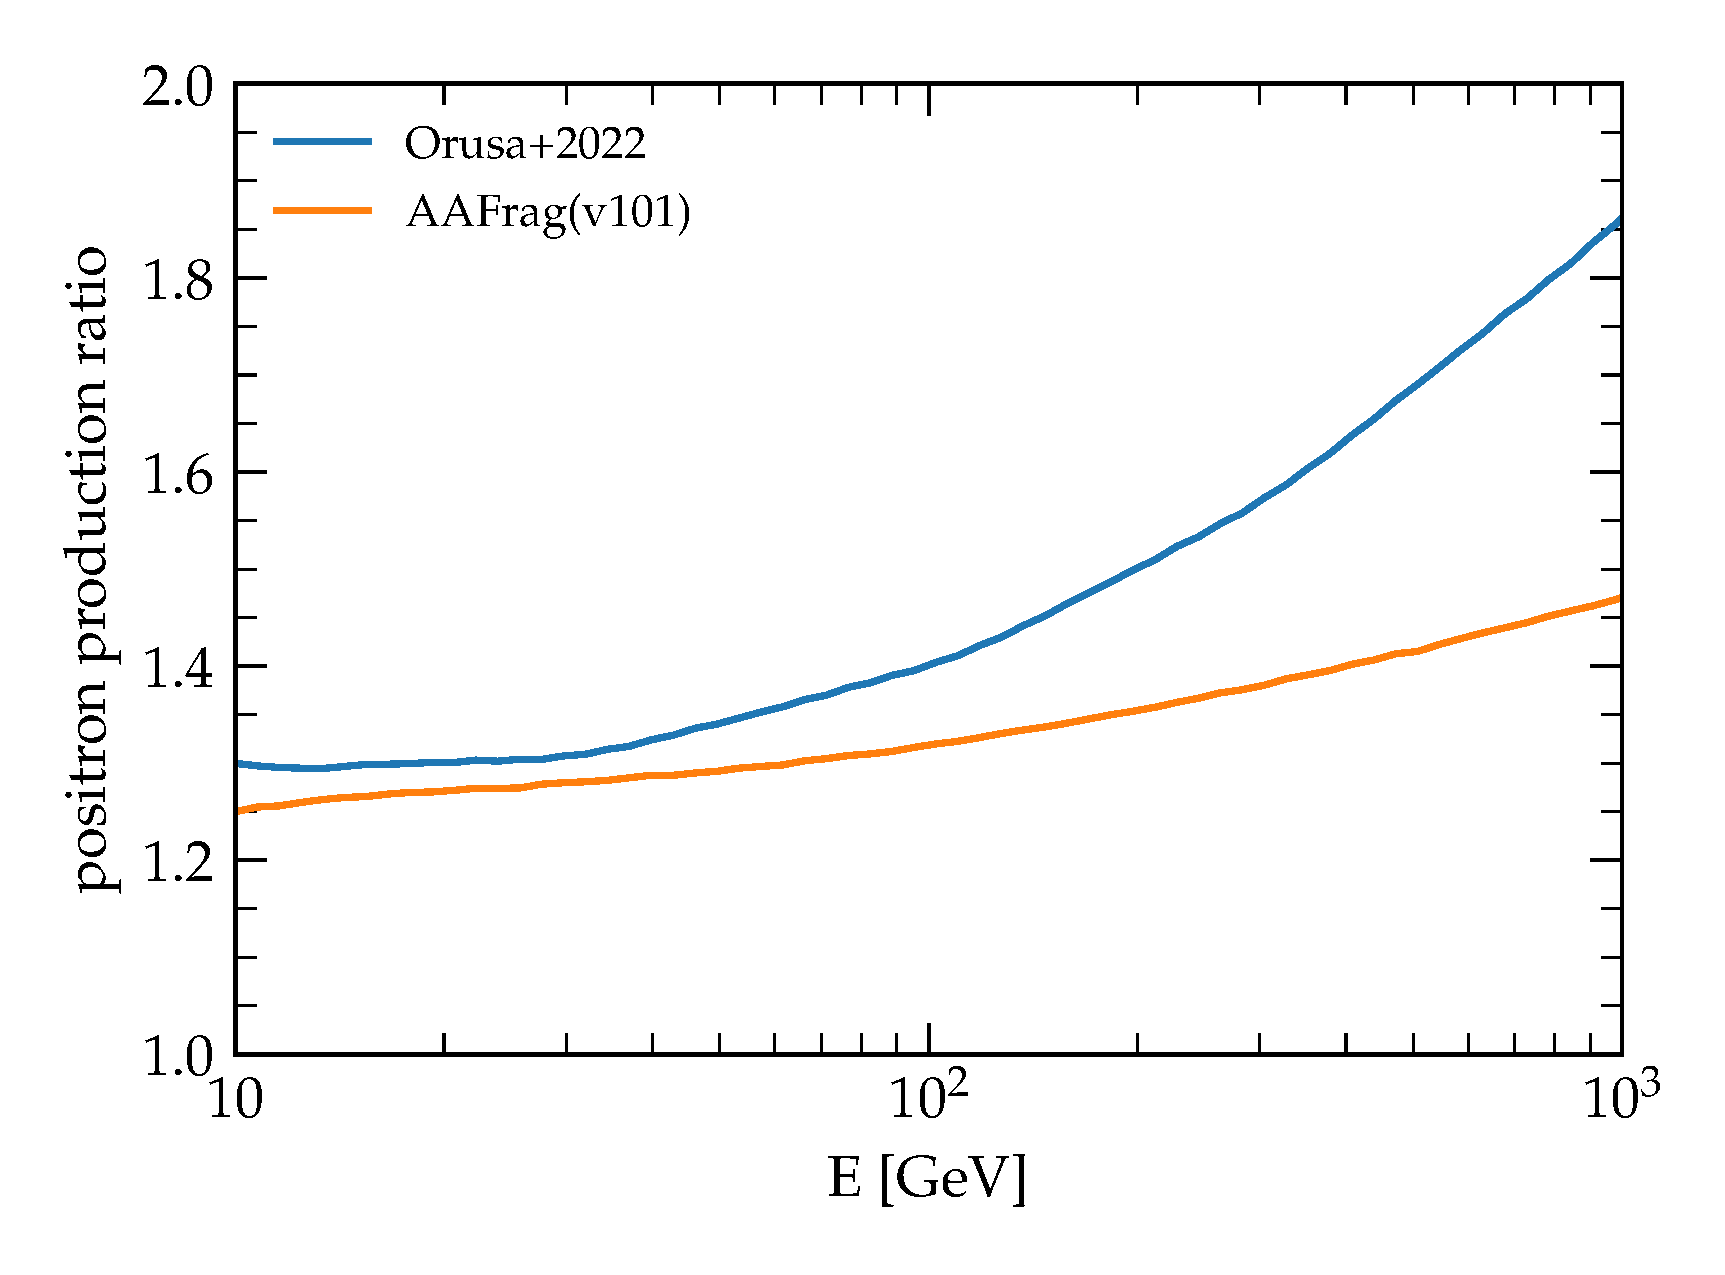
\includegraphics[width=0.6\textwidth]{figures/positron_source_term.pdf}
\caption{The positron production rate computed in two recent models~\cite{Kachelriess2019cpc,Orusa2022prd} normalized to the production rate in the constant-\emph{inelasticity} approach outlined in the text.}
\label{fig:positronsourceratio}
\end{figure}

This is different from the case of B/C, where carbon was the parent of boron,  as here electrons are not parents of secondary electrons.
%
Notwithstanding, assuming $\gamma_p \simeq \gamma_e$, the positron fraction is a decreasing function with energy, approximately following $E^{-\delta}$.

In figure~\ref{fig:positronfraction}, we present the positron fraction as a function of energy, which markedly deviates from the expectation for pure secondary production above $\sim$10 GeV.

Following equation~\eqref{eq:positronfractiontheory}, for the positron fraction to increase with energy, it would require $\gamma_e > \gamma_p + \delta$, which is highly unlikely!

Another possibility we may consider to explain the anomaly in the positron fraction is a significant modification of the cross-sections involved in secondary production processes.
%
Recent efforts have been made to re-evaluate these cross-sections by fitting data from collider experiments or by utilizing hadronic interaction models~\cite{Orusa2022prd,Kachelriess2019cpc}. The production rates obtained using these approaches can be compared with the rates predicted by equation~\eqref{eq:positronproduction}, as shown in figure~\ref{fig:positronsourceratio}. 
%
The comparison reveals that there are no deviations from our initial naive approach at a level that would account for the observed excess.

As such, we are left with no other option than to postulate the existence of a new population of positron sources in the Universe!

% !TEX root = ./main.tex
\section{Immediate implications of cosmic ray observations}
\label{sec:implications}

\subsection{Efficiency of particle acceleration in Galactic sources}

In the previous sections, we have discussed how the abundances of certain elements such as boron, lithium and beryllium in CRs provide us with valuable estimates of the time $\tau_{\rm esc}$ that CRs spend in the Galaxy before escaping.
%
Now, we delve deeper into the implications of these observations, specifically focusing on the energetic budget required by galactic sources to sustain the CR population.

Having in mind acceleration mechanisms similar to DSA, to describe the injection spectrum of protons, we assume a power-law form in momentum that accounts for both relativistic and non-relativistic particles:
%
\begin{equation}
N(p) = N_0 \left(\frac{p}{m c}\right)^{-\gamma} \, , 
\end{equation}
%
where $\gamma \gtrsim 4$. The normalization of $N(p)$ is determined by the condition that the integrated energy in particles matches the energy released in CRs by a single event:
%
\begin{equation}
4 \pi \int_0^\infty dp \, p^2 N(p) T(p) = E_{\rm CR}
\end{equation}

Solving for $N_0$, we find
%
\begin{equation}
N_0 = \frac{E_{\rm CR}}{4 \pi c (m c)^4 I(\gamma)},
\end{equation}
where $I(\gamma) = \int_0^\infty dx \, x^{2-\gamma} \left[ \sqrt{x^2+1} - 1 \right]$.

Note that due to spectral index values larger than 4, the total energy budget is determined by protons with energies of $\sim$GeV, and we can ignore the existence of minimum and maximum momentum.

Assuming high energies where ionization losses can be neglected and solar modulation has no significant effect, the proton spectrum contributed by identical sources occurring at a rate $\mathcal R$ can be expressed as:
%
\begin{equation}
f_{\rm p}(p) = \frac{E_{\rm CR} \mathcal R}{8 \pi^2 R_{\rm d}^2 c (m c)^4 I(\gamma)} \left( \frac{p}{mc}\right)^{-\gamma} \frac{H}{D(p)},
\end{equation}

Using the definition of intensity, given in appendix~\ref{app:intensity}, and considering that in the relativistic limit $E \simeq p c$, we obtain:
%
\begin{equation}
I_{\rm p}(E) = \frac{E_{\rm CR} \mathcal R c}{8 \pi^2 R_{\rm d}^2 (m c^2)^2 I(\gamma)} \left( \frac{E}{mc^2}\right)^{2-\gamma} \frac{H}{D(E)}
\end{equation}
%
which gives for $E = 10$~GeV:
%
\begin{equation}
E^2 I_{\rm p}(E) \simeq 2 \times 10^3 \left(\frac{E_{\rm CR} \mathcal R}{10^{40} \, \text{erg} \, \text{s}^{-1}}\right) \, \text{GeV} \, \text{m}^{-2} \, \text{s}^{-1} \, \text{sr}^{-1}
\end{equation}

\begin{figure}[t]
\centering
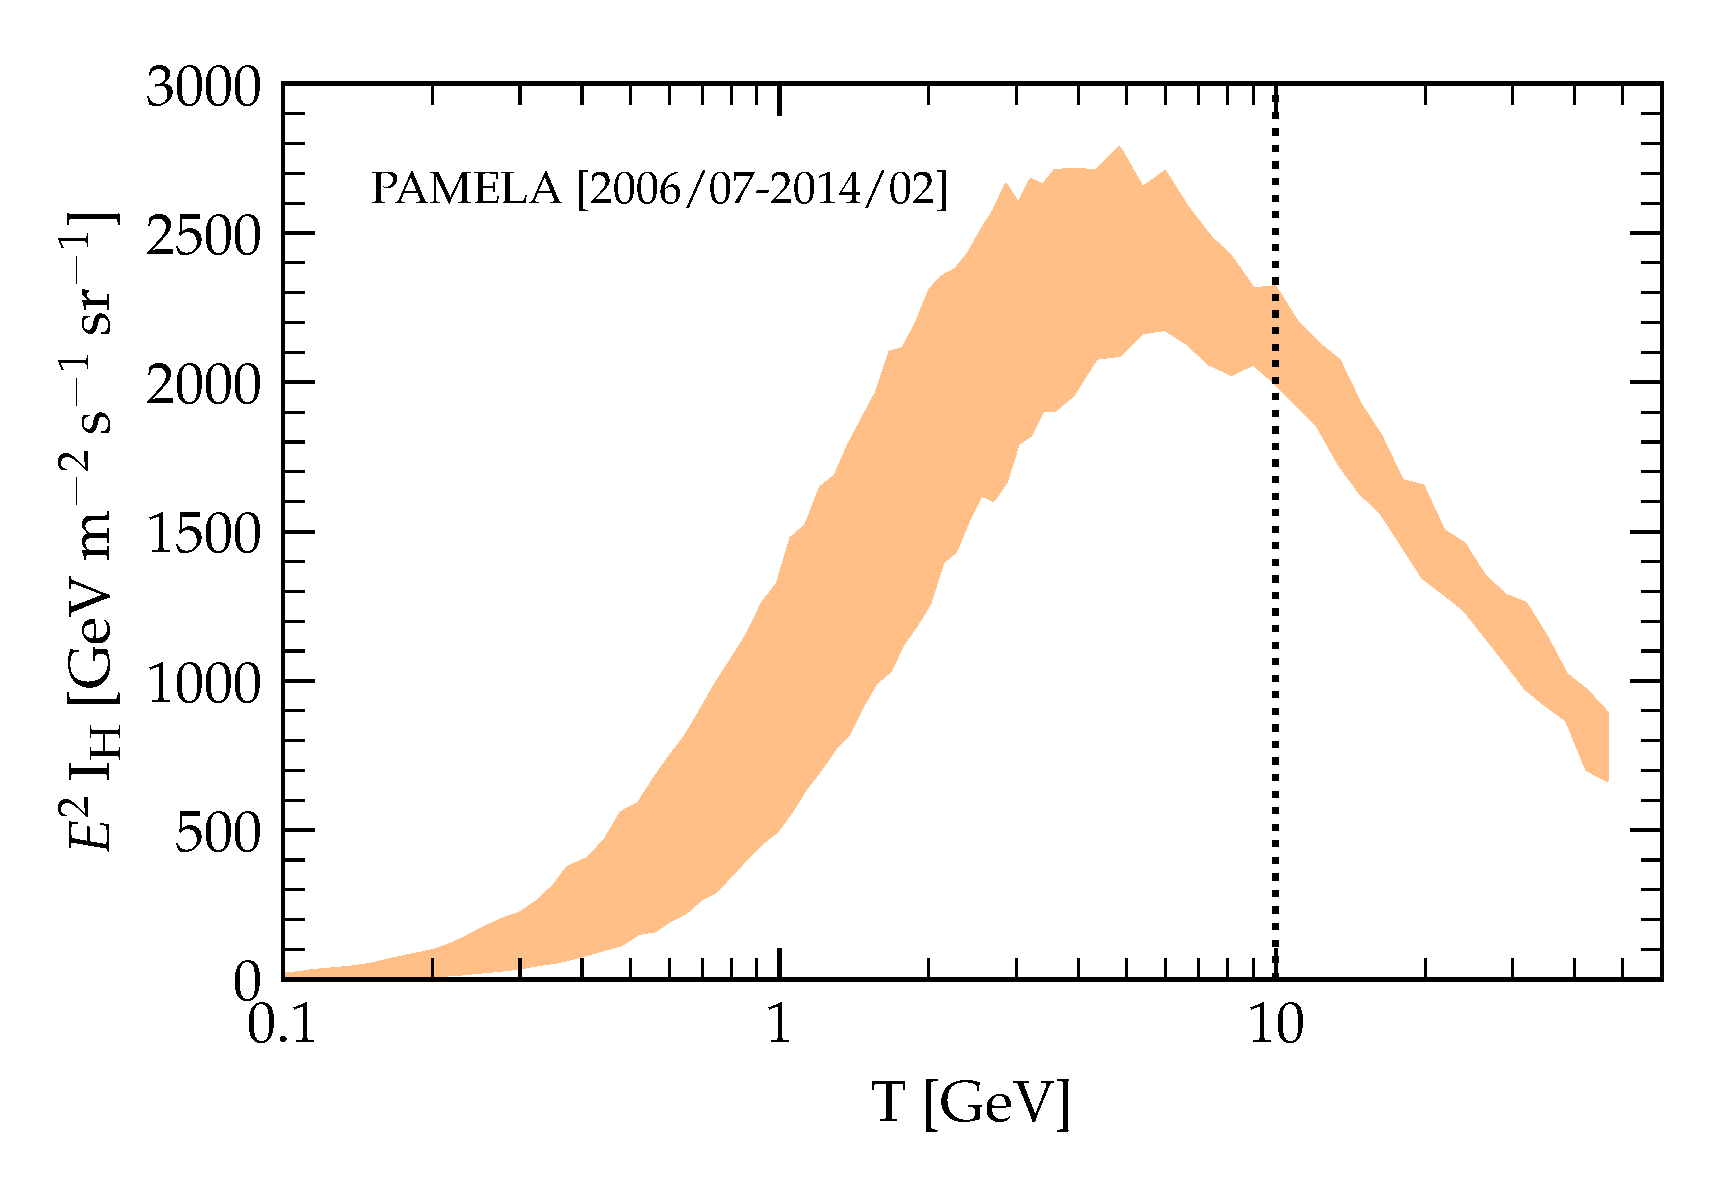
\includegraphics[width=0.6\textwidth]{figures/protons_le.pdf}
\caption{The proton intensity measured by the PAMELA experiment over a large fraction of the Solar activity cycle ~\cite{PAMELA.2011.proton}.}
\label{fig:pamelaprotons}
\end{figure}

By comparing this equation with the proton flux measured by the PAMELA experiment, as shown in figure~\ref{fig:pamelaprotons}, we find that in order to maintain a steady-state, the power that Galactic sources inject into the Galaxy in the form of CR protons needs to be approximately $\mathcal L \simeq E_{\rm CR} \mathcal R \simeq 10^{40} \text{erg} \, \text{s}^{-1}$ for a time not smaller than $\tau_{\rm esc}$.

Assuming that CRs are produced by supernova explosions with a rate of about 2 per century and with a typical mechanical energy release of $10^{51}$ erg per explosion, the luminosity amounts to $6 \times 10^{41}$ erg/s, significantly exceeding the required one. Hence, it is necessary to invoke an efficiency of a few percent in the conversion between supernova kinetic energy and CR energy to make this hypothesis viable.

Detailed calculations provide a more accurate estimate of the total acceleration efficiency, typically ranging from 5\% to 10\% (including nuclei), for the majority of supernova remnants. This efficiency is well described in recent models of diffusive shock acceleration~\cite{Morlino2017hsn}, upraising the hypothesis that CRs acquire their energy from Galactic stellar explosions to the rank of a \emph{paradigm}.

Over the years, alternative sources of energy, such as those in the Galactic Center region, star clusters, or OB associations\footnote{OB associations consist largely of very young, massive stars (about 10 to 50 solar masses) of spectral types O and B.}, have been proposed to explain galactic CRs. 
%
Interestingly, the star clusters scenario for the origin of galactic CRs have recently gained renewed attention based on gamma-ray observations (see S.~Gabici's lecture notes in this volume).

%%% SI PUO STIMARE L'EFFICIENZA IN SNE, vedi Morlino review.

\subsection{Constraints on the microphysics of galactic transport}

In the previous sections, we have discussed how the remarkable longevity of CRs, which greatly exceed the time it would take them to propagate freely at the speed of light, suggests that CRs undergo a random walk, continually scattered as they traverse their path from the sources to Earth.
%
Furthermore, the absence of a strong anisotropy, $\mathcal{O}(1)$, toward the galactic center for CRs with energies below $10^{15}$ eV implies that multiple scatterings wash out the anisotropy that would be expected if there were no scattering~\cite{Hillas2005jpg}. 

The scattering cannot be attributed to ISM nuclei, as the mean free path for Coulomb collisions of relativistic nucleons in the dilute ISM, given by $\lambda \simeq \frac{1}{n_{\rm H} \sigma_{\rm T}} \sim 10^{24}$ cm, is far too long.

Hence, the most likely scattering mechanism is the interaction of CRs with plasma waves, which are fluctuating electromagnetic fields in the ISM. The presence of a random component of the Galactic magnetic field is inferred from fluctuations in rotation measures, combined with estimates of thermal electron density and synchrotron depolarization. Recent analyses have reported a strength of this component at around $1-3 \mu$G~\cite{Ferriere2023epj}.

Understanding the production of these plasma waves and their influence on the dynamics of CR particles is a crucial topic in the theoretical investigation of CR physics.

Typically, the energy spectrum of the turbulent field is assumed to follow a power-law distribution with an outer scale of $L \sim 10$ pc, where energy is injected. This energy then cascades down to smaller scales until it dissipates at the dissipation scale.

For CR nuclei in the GeV-TeV energy range and charge $Z$, the Larmor radius in this magnetic field is given by:
%
\begin{equation}
r_{\rm L} \simeq 10^{-5} \, \text{pc} \left( \frac{E / Z}{10 \, \text{GeV}} \right) \left( \frac{B}{\mu\text{G}}\right)^{-1}  
\end{equation}

This length scale is much smaller than the random field injection scale but larger than the dissipation scale. Consequently, a CR nucleus is expected to encounter numerous magnetic scattering centers before reaching Earth.

This transport mechanism is understood in terms of resonant wave-particle interaction, where CRs primarily scatter off waves with wavelengths comparable to their gyroradius. 

Under these conditions, a particle interacts with a wave remaining in phase with the wave over many cycles. 
%
This scattering leads to an effective diffusion in pitch angle which, in turn, regulates their diffusion in real space.

The resonant condition can be expressed as
%
\begin{equation}
k_{\rm res} = \frac{1}{\mu r_{\rm L}}
\end{equation}
%
where $k_{\rm res}$ represents the wavelength of the \emph{resonant} magnetic perturbation and $\mu$ is the cosine of the particle's pitch angle.

Within quasilinear theory the spatial diffusion coefficient results from the pitch-angle-cosine $\mu$ average of the inverse of the pitch-angle diffusion coefficient $D_{\mu\mu}$ (see appendix~\ref{app:diffusioncoefficient}):
%
\begin{equation}
D \simeq \frac{(1-\mu^2) v^2}{D_{\mu\mu}}
\label{eq:dandbasta}
\end{equation}

The pitch-angle diffusion rate must depend upon the distribution of wave energy, and in weakly turbulent magnetic fields, we obtain:
%
\begin{equation}
D_{\mu\mu} \simeq \pi \Omega (1-\mu^2) k_{\rm res} \mathcal F(k_{\rm res})
\label{eq:dmumusimeq}
\end{equation}
%
where $\Omega = c / r_{\rm L}$ is the gyrofrequency, and $\mathcal F$ is the power in modes of wavenumber $k_{\rm res}$ normalized such that its integral gives the fraction of energy density in the turbulent components with respect to the regular field:
%
\begin{equation}
\int_{1/L}^\infty \! dk \, \mathcal F(k) = \frac{\langle \delta B^2 \rangle}{B_0^2}
\end{equation}

Intuitively, if we associate the angle by which the fieldlines are bent $\delta B/B_0$ with the scattering angle $\delta \theta$, and assume the particles encounter uncorrelated waves at frequency $\Omega$, then the angular diffusion coefficient is $\langle (\delta \theta)^2 \rangle / \delta t \sim \Omega (\delta B/B_0)^2$ which is essentially equation~\eqref{eq:dmumusimeq}. 

Combined with equation~\eqref{eq:dandbasta} the diffusion coefficient reads
%
\begin{equation}
D \simeq \frac{1}{3} r_{\rm L} c \frac{1}{k_{\rm res} \mathcal F(k_{\rm res})}
\label{eq:dzz}
\end{equation} 

We recall now from equation~\eqref{eq:grammage} that the best fit to secondary-over-primary CRs in the Galaxy indicates a diffusion coefficient of $D/H \sim 2$ for particles around 10 GeV, where $D$ is measured in units of $10^{28}$ cm$^2$ s$^{-1}$ and $H$ represents the scale height in kpc. 
%
Combining this information with the determination of the halo size obtained from unstable species, $H \sim 5$ kpc, we obtain a \emph{measurement} of the normalization of the diffusion coefficient to be approximately $D \sim 10^{29}$ cm$^2$ s$^{-1}$.

%DIRE QUI DEL MFP? {\color{magenta}{Ti riferisci alla condizione che il mean free path deve essere molto piu' piccolo rispetto alle dimensioni di H? Sarebbe interessante dedicargli un paragrafetto}}

By inverting equation~\eqref{eq:dzz}, we can finally determine the required level of turbulence at the scale of 10 GeV particles in order to replenish the observed amount of secondary particles:
%
\begin{equation}
k_{\rm res} \mathcal F(k_{\rm res}) \simeq \text{few} \times 10^{-6}
\end{equation}

In summary, even such a small perturbation at a scale corresponding to the size of the solar system, $\sim$A.U., is enough to significantly extend the transport time of CRs in the Galaxy from thousands of years to millions of years!


\newpage

\appendix

\newpage
\chapter{Appendix}
% !TEX root = ../main.tex
\section{Motion of a Charged Particle in a Constant Magnetic Field}

Let's start from the Lorentz force
%
\begin{equation*}
\frac{d}{dt} \left( m \gamma \vb v\right) = q \frac{\vb v}{c} \times \vb B \longrightarrow m \gamma \frac{d\vb v}{dt} = \frac{q}{c} \, \vb v \times \vb B
\end{equation*}
%
where I used the fact that in the absence of electric fields, $\gamma$ is constant with time % (in fact, $d/dt(\gamma m c^2) = q \vec v \cdot \vec E$)

The projection along $z$ of $\vb v \times \vb B$ is null, therefore
%
\begin{equation*}
m \gamma \frac{d}{dt} v_z = \frac{d}{dt} p_z = 0
\end{equation*}

% $\frac{d}{dt} v_z = 0$ and $v_z =$~const and $p_z = m \gamma v_z =$~const

from this it follows $p_z / p = \mu =$~const (is the \emph{pitch angle}) and 
%
\begin{equation*}
p_\perp = (p^2 - p_z^2)^{1/2} = (p_x^2 + p_y^2)^{1/2} = (1-\mu^2)^{1/2} =~\text{const}
\end{equation*}

in the orthogonal projection
%
\begin{equation*}
m \gamma \frac{d}{dt} v_\perp = \frac{q}{c} v B \sin \theta = \frac{q v_\perp B}{c}  
\longrightarrow \frac{d}{dt} v_\perp = \frac{q v_\perp B}{m \gamma c}  = \frac{v_\perp^2}{r_{\rm L}}
\end{equation*}
%
where I introduced the \emph{Larmor radius}:
%
\begin{remark}
\[
r_{\rm L} = \gamma r_g = \frac{{\color{red}\gamma} m c  v_\perp}{q B} \simeq \frac{\gamma m c^2}{qB}
\]
\end{remark}
%
notice that this is the same as the gyro-radius with the difference of this $\gamma$ factor

(reminder: centripetal force is $\frac{m v_\perp^2}{r_g}$)

The corresponding Larmor angular frequency is
%
\begin{equation*}
\Omega_{\rm L} = \frac{v_\perp}{r_{\rm L}} = \frac{qB}{\gamma m c} = \frac{\Omega_0}{\gamma}
\end{equation*}

The equation of motion after integrating becomes
%
\begin{eqnarray}
v_x & = & v_\perp \cos \left(\Omega t\right) \\
v_y & = & v_\perp \sin \left(\Omega t\right) \\
v_z & = & v \mu
\end{eqnarray}
%
and for the trajectory
%
\begin{eqnarray}
x(t) & = & x_g + r_L \sin \left(\Omega t\right) \\
y(t) & = & y_g + r_L \cos \left(\Omega t\right) \\
z(t) & = & z_g + v \mu t
\end{eqnarray}

where $(x_g, y_g, z_g)$ are the coordinates of the guiding centre.

Recap of quantity defined here: 
%
\begin{center}
\begin{tabular}{|l|c|c|}
\toprule
radius & $r_g = \frac{m c v_\perp}{qB}$ & $r_L = \gamma r_g$ \\
angular frequency & $\Omega_0 = \frac{v_\perp}{r_g} = \frac{qB}{m c}$ & $\Omega_L =  \frac{v_\perp}{r_L} = \frac{\Omega_0}{\gamma} $\\
frequency & $\nu_g = \frac{\Omega_0}{2\pi} = \frac{qB}{2 \pi m c}$ & $\nu_L =  \frac{\nu_g}{\gamma} $\\
\bottomrule
\end{tabular}
\end{center}


% !TEX root = ../main.tex
\section{The Radiative Transfer Equation}

Radiative transfer involves understanding how radiation propagates and interacts with matter. 

The flux density \( F \) is defined as the energy flux density, \( F = \frac{dE}{dA dt} \), where \( dA \) is the differential area. The \emph{specific} energy flux density \( F_\nu \) is given by \( F_\nu = \frac{dE}{dA dt d\nu} \), leading to \( F = \int d\nu F_\nu \).

Energy conservation in radiative transfer implies that the energy across different surfaces of the flux tube remains constant (\( dE_2 = dE_1 \)), where 1(2) denotes a surface at distance $r_1(r_2)$ leading to the relation:
%
\[
4 \pi r_2^2 F(r_2) = 4 \pi r_1^2 F(r_1) \rightarrow F(r) = \frac{F(r_1) r_1^2}{r_2^2} = \frac{\mathcal L}{4\pi r^2} 
\]
%
where \( \mathcal L \) represents the luminosity of the source.

Specific intensity \( I_\nu \) is the radiation intensity within a frequency band \( \nu \rightarrow \nu + d\nu \):
%
\[
dE = I_\nu dA dt d\Omega d\nu \rightarrow I_\nu = \frac{F_\nu}{d\Omega}
\]

This quantity depends on location, direction, and frequency, with the total intensity given by \( I = \int d\nu I_\nu \).

Why specific intensity is a convenient quantity? 

PLOT

The energy passing trough is $dE_1 = I_{\nu_1} dA_1 dt d\Omega_1 d\nu_1$, and $dE_2 = I_{\nu_2} dA_2 dt d\Omega_2 d\nu_2$

Assuming $d\nu_1 = d\nu_2$, and $d\Omega_{1} = \frac{dA_2}{R^2}$ and similarly $d\Omega_2 = \frac{dA_1}{R^2}$, the energy conservation $dE_1 = dE_2$ gives
%
\[
I_{\nu_1} dA_1 dt \frac{dA_2}{R^2} d\nu = I_{\nu_2} dA_2 dt \frac{dA_1}{R^2} d\nu \rightarrow I_{\nu_1} = I_{\nu_2}
\]
%
or 
%
\begin{remark}
\[
\frac{dI_\nu}{ds} = 0
\]
\end{remark}

It implies that all rays passing trough $A_1$ are also passing trough $A_2$, in other words, spectral intensity is the same \emph{at the source} and \emph{at the detector}.

The radiative energy density is the energy per unit volume per unit frequency range per unit solid angle
%
\[
dE = u_\nu(\Omega) dV d\Omega d\nu
\]
%
for light $dV = (c dt) dA \rightarrow dE = c u_\nu dt dA d\Omega d\nu \rightarrow u_\nu = \frac{I_\nu}{c}$

The specific energy density
%
\[
u_\nu = \int d\Omega u_\nu(\Omega) = \frac{1}{c} \int d\Omega I_\nu(\Omega) = \frac{4\pi}{c} J_\nu
\]
%
where $J$ is the mean intensity
%
\[
J_\nu = \frac{1}{4\pi}\int d\Omega I_\nu(\Omega) 
\]
%
for an isotropic field is $J_\nu = I_\nu$.

The total energy density is
%
\[
u = \int d\nu u_\nu = \frac{4\pi}{c} \int d\nu J_\nu
\]

{\color{red}TO BE FINISHED...}

%EEE
%
%The emission and absorption of radiation can change the specific intensity. The emission is quantified by the spontaneous emission coefficient \( j_\nu \), which represents the energy added per unit volume, solid angle, time, and frequency. Absorption is described by the absorption coefficient \( \alpha_\nu == n \sigma_\nu \), where \( n \) is the number density of absorbers, and \( \sigma_\nu \) is the cross-sectional area of an absorber.
%
%EEE
%
%**Radiative Transfer Equation:**
%
%The master equation of radiative transfer combines these two processes:
%
%\[
%\frac{dI_\nu}{ds} = j_\nu - \alpha_\nu I_\nu
%\]
%
%**Optical Depth and Mean Free Path:**
%
%The optical depth \( \tau_\nu \) is a measure of the transparency of the medium:
%
%\[
%\tau_\nu (s) = \int_0^s ds' \alpha_\nu(s') = n \sigma_\nu s
%\]
%
%The medium is defined as optically thick if \( \tau_\nu > 1 \) or optically thin if \( \tau_\nu < 1 \). The mean free path \( \lambda \) is the average distance a photon travels before being absorbed or scattered, given by \( \lambda = \frac{1}{n \sigma_\nu} \).
%
%**Formal Solution and Source Function:**
%
%The formal solution to the transfer equation is:
%
%\[
%I_\nu (\tau_\nu) = I_\nu(0) \exp(-\tau_\nu) + \int_0^{\tau_\nu} d\tau'_\nu \exp\left[ -(\tau_\nu - \tau'_\nu) \right] S_\nu(\tau'_\nu)
%\]
%
%where \( S_\nu = \frac{j_\nu}{\alpha_\nu} \) is the source function. This function represents the balance of emission and absorption processes within the medium.
%
%---
%
%
%Emission and absorption can change $I_\nu$
%
%Emission: radiation can be emitted \emph{adding energy} to the beam
%%
%\[
%dE_{\rm in} = j_\nu dV d\Omega dt d\nu \rightarrow j_\nu = \frac{dE_{\rm in}}{dV d\Omega dt d\nu}
%\]
%%
%where $j_\nu$ is the \emph{spontaneous emission coefficient}, namely energy added per unit volume, unit solid angle, unit time and unit frequency.
%
%In going a distance $ds$, a beam of cross section $dA$ travels through a volume $dV=dA ds$, therefore
%%
%\[
%d I_\nu = \frac{dE_{\rm in}}{dA d\Omega dt d\nu} = j_\nu ds
%\]
%
%Absorption: radiation can be absorbed \emph{taking away energy} from the beam
%
%The number of absorbers is $n dV$ where $n$ is the absorber number density, therefore the total absorbing area is $n dV \sigma_\nu = dA_{\rm abs}$
%
%The energy removed from the beam is
%%
%\[
%dE_{\rm out} = - I_\nu dA_{\rm abs} d\Omega dt d\nu = -  I_\nu n \sigma_\nu ds dA  d\Omega dt d\nu  
%\]
%%
%or
%%
%\[
%d I_\nu = \frac{dE_{\rm out}}{dA d\Omega dt d\nu} =\frac{I_\nu n \sigma_\nu ds dA  d\Omega dt d\nu}{dA d\Omega dt d\nu} = I_\nu n \sigma_\nu ds 
%\]
%
%The master equation of radiation transfer is derived from $dI_\nu = dI_\nu - dI_\nu$, that is
%%
%\begin{remark}
%\[
%\frac{dI_\nu}{ds} = j_\nu - \alpha_\nu I_\nu
%\]
%\end{remark}
%%
%where $\alpha_\nu = n \sigma_\nu$ and is know as \emph{absorption coefficient}.
%
%A trivial solutions:
%
%Case pure emission: $\alpha_\nu = 0$ follows
%%
%\[
%I_\nu (s) = I_\nu (0) + \int_0^s ds' j_\nu(s')
%\]
%
%Case pure absorption: $j_\nu = 0$ follows
%%
%\[
%I_\nu(s) = I_\nu (0) \exp \left[ -\int_0^s ds' \alpha_\nu(s') \right] = I_\nu(0) \exp(-\tau_\nu) 
%\]
%
%It is useful to introduce the optical depth 
%%
%\[
%\tau_\nu (s) = \int_0^s ds' \alpha_\nu(s') = n \sigma_\nu s
%\]
%%
%where the last is valid only if $n$ is constant
%
%The mediums is defined \emph{optically thick} if $\tau_\nu > 1$ or \emph{optically thin} if $\tau_\nu < 1$
%
%The optical depth is useful to introduce the \emph{mean free path}
%
%From the exponential absorption law, the probability of a photon traveling at least an optical depth $\tau_\nu$ is simply $\exp(-\tau_\nu)$, follows that the mean optical depth traveled is equal to unity:
%%
%\[
%\langle \tau_\nu \rangle = \int_0^\infty d\tau_\nu \tau_\nu \exp(-\tau_\nu) = 1
%\]
%
%The mean distance traveled in a homogeneous medium is defined as $1 = \langle \tau_\nu \rangle = \alpha_\nu \lambda$, from which follows
%%
%\begin{remark}
%\[
%\lambda = \frac{1}{n \sigma_\nu}
%\]
%\end{remark}
%
%In terms of the optical depth the transfer equation can be written 
%%
%\[
%\frac{dI_\nu}{ds} =  j_\nu - \alpha_\nu I_\nu \rightarrow 
%\alpha_\nu \frac{dI_\nu}{d\tau_\nu} =  j_\nu - \alpha_\nu I_\nu \rightarrow 
%\frac{dI_\nu}{d\tau_\nu} =  S_\nu - I_\nu  
%\]
%%
%where $S_\nu = \frac{j_\nu}{\alpha_\nu}$ is the Source function.
%
%The formal solution of the transfer equation reads
%%
%\[
%I_\nu (\tau_\nu) = I_\nu(0) \exp(-\tau_\nu) + \int_0^{\tau_\nu} d\tau'_\nu \exp\left[ -(\tau_\nu - \tau'_\nu) \right] S_\nu(\tau'_\nu)
%\]
%%
%follows \emph{interpretation}.
%
%For constant source function
%%
%\[
%I_\nu (\tau_\nu) 
%%= I_\nu(0) \exp(-\tau_\nu) + S_\nu \int_0^{\tau_\nu} d\tau'_\nu \exp\left[ -(\tau_\nu - \tau'_\nu) \right] 
%= I_\nu(0) \exp(-\tau_\nu) + S_\nu \left[1 - \exp(-\tau_\nu)\right]
%\] 

%\item Example: how is it defined the thermodynamic equilibrium? Where the ratio between emissivity and absorption is 
%%
%\begin{equation*}
%B_\nu(T) = \frac{2h\nu^3}{c^2} \frac{1}{\exp(h\nu/kT) - 1}
%\end{equation*}


% !TEX root = ../lectures.tex
%%%%%%%%%% SECTION %%%%%%%%%
\section{The Cosmic Ray Intensity}  
\label{app:intensity}

In this appendix, we provide an introduction to the key definitions used to describe the density and intensity of cosmic rays (CRs). These concepts are essential for connecting CR measurements and their physical implications.  

The starting point for describing the cosmic ray density is the \emph{distribution function}, \(\phi(\vb{r}, \vb{p}, t)\), which represents the number of particles in a small spatial volume \(d^3 \vb{r}\) around \(\vb{r}\) and within a momentum interval \(d^3 \vb{p}\) around \(\vb{p}\):  
\begin{equation}
d\rho = \phi(\vb{r}, \vb{p}, t) \, d^3 \vb{r} \, d^3 \vb{p}.
\end{equation}

To account for the geometry of momentum space, we rewrite \(d^3 \vb{p}\) in spherical coordinates as:  
\begin{equation}
d^3 \vb{p} = p^2 dp \, d\Omega,
\end{equation}
where \(p = |\vb{p}|\) is the magnitude of the momentum, \(dp\) is the infinitesimal momentum interval, and \(d\Omega\) represents the solid angle element. Substituting this into the expression for \(d\rho\) gives:  
\begin{equation}
d\rho = \phi(\vb{r}, p, t) \, d^3 \vb{r} \, p^2 dp \, d\Omega.
\end{equation}

In practice, it is often not possible to measure \(\phi(\vb{r}, \vb{p}, t)\) directly. Instead, measurements typically involve quantities averaged over the direction of \(\vb{p}\). For this reason, we define the \emph{phase-space distribution function} \(f(\vb{r}, p, t)\), which averages \(\phi(\vb{r}, p, t)\) over all directions:  
\begin{equation}
f(\vb{r}, p, t) = \frac{1}{4\pi} \int_\Omega \phi(\vb{r}, p, t) \, d\Omega.
\end{equation}

Using this definition, the number of particles in a spatial volume \(d^3 \vb{r}\) and within a momentum interval \(dp\), regardless of the direction of \(\vb{p}\), is given by:  
\begin{equation}\label{eq:dnd3p}
dn = 4\pi p^2 f(\vb{r}, p, t) \, d^3 \vb{r} \, dp.
\end{equation}

It is important to emphasize here that if the phase-space distribution function scales with momentum as
\begin{equation}
f \propto p^{-\gamma}~,
\end{equation}
then the corresponding number density \( n\), when expressed as differential in energy \( E\), is:
\begin{equation}
n(E) dE = n(p) dp = 4 \pi p^2 f(\vb{r}, p, t) \, dp~,
\end{equation}
%
thus, for relativistic particles, it scales as
\begin{equation}
n(E) \propto E^{2-\gamma}~.
\end{equation}

This relationship arises because the conversion from momentum to energy introduces an additional factor of \(p^2\) due to the geometry of momentum space. Consequently, the spectral index in energy space is shifted by 2 compared to the spectral index in momentum space.  

\subsection{Differential Intensity}

Experimental measurements of cosmic rays are usually reported in terms of the \emph{differential intensity}, \(I\), which is defined as the number of particles detected per unit energy, unit area, unit time, and unit solid angle. This quantity provides a direct way to compare observed cosmic ray spectra.  

Moreover, for convenience, CR spectra are often expressed as a function of the \emph{kinetic energy per nucleon}, \(T\). This choice is particularly useful because \(T\) remains approximately conserved when a nucleus undergoes fragmentation in interactions with interstellar gas.  

The intensity of a specific nuclear species \(\alpha\) can be related to the phase-space distribution \(f_\alpha(p)\). 
%
For a given kinetic energy interval \(dT\), the differential intensity, using equation~\eqref{eq:dnd3p}, is:  
\begin{equation}
I_\alpha(T) \, dT = c \, p^2 \, f_\alpha(p) \, \beta(p) \, dp,
\end{equation}
where \(\beta(p) \) is the particle’s velocity expressed as a fraction of the speed of light, and \(p\) is the momentum corresponding to the kinetic energy \(T\).  

Reminding that \( \frac{dp}{dT} = \frac{A}{v} \), this expression can be further simplified as:  
\[
I_\alpha(T) = A \, p^2 \, f_\alpha(p),
\]  
where \(A\) is the nuclear mass.

% !TEX root = ../main.tex
\section{Thermodynamics of Adiabatic Processes}

An adiabatic process is defined by the absence of heat transfer to or from the system \( \delta Q = 0 \). According to the first law of thermodynamics:
\begin{equation}
\label{eq:firstlaw}
d\mathcal U + PdV = 0
\end{equation}
This equation implies that any work (\(PdV\)) performed must be compensated by a change in the internal energy (\(\mathcal U\)), as no heat is exchanged with the surroundings.

For an ideal gas, obeying the equation of state \(PV = nRT\) (where \(R\) is the universal gas constant), the internal energy is given by:
\begin{equation}
\label{eq:nrt} 
\mathcal U = \alpha n R T = \alpha PV 
\end{equation}
Here, \(n\) represents the number of moles, and \( \alpha \) is the number of degrees of freedom divided by 2.

Differentiating Equation~\ref{eq:nrt} results in:
\begin{equation}\label{eq:dunrdt}
d\mathcal U = \alpha n R dT = \alpha (P dV + V dP)
\end{equation}

Substituting this into Equation~\ref{eq:firstlaw} yields:
\begin{equation}
- PdV = \alpha P dV + \alpha V dP \rightarrow -(\alpha + 1) \frac{dV}{V} = \alpha \frac{dP}{P}
\end{equation}

Integrating both sides of this equation, we get:
\begin{equation}
\ln \left( \frac{P}{P_0} \right) = - \frac{\alpha + 1}{\alpha} \ln \left( \frac{V}{V_0} \right) = - \gamma_g \ln \left( \frac{V}{V_0} \right)
\end{equation}
where \( \gamma_g \) is the heat capacity ratio, \( c_V = \alpha R \), and we have used Mayer's relation \(c_P - c_V = R\).

Thus, a reversible adiabatic process (one with no entropy generation) can be characterized by the polytropic process equation:
\begin{remark}
\begin{equation}
PV^\gamma = \text{constant}
\end{equation}
\end{remark}
%%% END CGPT

Notice that for an ideal gas the \emph{internal energy} is solely a function of temperature. Indeed, from Eq.~\ref{eq:nrt}, we obtain 
\begin{equation}
\mathcal U = n c_V T = \frac{PV}{\gamma_g - 1}
\end{equation}

Thus, expressing internal energy per unit volume as \(u\), we get:
%
\begin{equation}
u = \frac{\mathcal U}{V} = \frac{P}{\gamma_g - 1}
\end{equation}

On the other hand, \emph{enthalpy} \( \mathcal H\) is defined as:
\[
\mathcal H = \mathcal U + PV \rightarrow  \frac{\mathcal H}{V} = u + P
\]

Employing the relation \(u = \rho \epsilon\) (where \(\rho\) is the density and \(\epsilon\) is the \emph{specific} internal energy, i.e., energy per unit mass), we derive the \emph{specific} enthalpy:
\begin{remark}
\begin{equation}
h = \frac{1}{\rho} \frac{\mathcal H}{V} = \epsilon + \frac{P}{\rho}
\end{equation}
\end{remark}


%%% END

% Last the first law of thermodynamics states that
% \[
% dU=TdS-PdV
% \]
% with $S$ the entropy,  which is conserved (so $dS=0$).  If we divide by mass we obtain the specific quantities,  namely
% \[
% d\epsilon=-Pd\left(\frac{1}{\rho}  \right)
% \]
%
% Therefore:
% \[
% dw = d\epsilon +\frac{dP}{\rho}+P d\left(\frac{1}{\rho}  \right)=\frac{dP}{\rho}
% \]
%
%
%Noting that $U = \frac{P}{\rho (\gamma − 1)}$ from ideal gas law, with $U$ internal energy per unit mass.
%
%Now introduce the entropy per unit mass $s$,  satisfying the adiabatic condition
%\begin{equation}
%\frac{\partial s}{\partial t} + u \frac{\partial s}{\partial z}=0
%\end{equation}
%Entropy per unit volume would be $\rho s$,  so that we can write (questa si puo derivare ma u e' costante o no?)
%\begin{equation}
%\frac{\partial (\rho s)}{\partial t}+\vec{\nabla}(\rho s\vec{u}) =0 \underset{1d}{\implies} \frac{\partial (\rho s)}{\partial t}+\frac{\partial}{\partial z}(\rho su) =0 
%\end{equation}
%
%The \textbf{enthalpy} of the system is \[ \mathcal W = E + PV \], while the specific enthalpy is \[ w=\epsilon +\frac{P}{\rho} \].
%
%Therefore
%\begin{equation}
%dw=d\epsilon +d\left(\frac{P}{\rho} \right)
%\end{equation}
%On the other hand
%\begin{equation}
%\begin{aligned}
% dE &= dQ-PdV\\
%&=\cancel{TdS} -PdV\\
%\implies d\epsilon &=-Pd\left(\frac{1}{\rho}\right)\\
%&=\frac{P}{\rho^2}d\rho
%\end{aligned}
%\end{equation}
%\begin{equation}
%\implies
%dw=\frac{P}{\rho^2}d\rho +\frac{dP}{\rho}-\frac{P}{\rho^2}d\rho =\frac{dP}{\rho}
%\end{equation}
%Now we can use again the conservation of momentum and write:
%\begin{equation}
%\frac{\partial u}{\partial t}+u\frac{\partial u}{\partial z}=-\frac{\nabla P}{\rho}\equiv \nabla \left[\epsilon +\frac{P}{\rho}  \right]
%\end{equation}
%Remember the energy density per unit volume
%\begin{equation}
%u=\frac{P}{\gamma_g -1}=\rho\epsilon \implies \epsilon =\frac{1}{\gamma_g -1}\frac{P}{\rho}
%\end{equation}
%

% !TEX root = ../main.tex
\section{Solving the Rankine-Hugoniot relations}

We are tasked with solving the following system of equations to understand shock wave dynamics:
%
\begin{eqnarray}
\rho_1 u_1 & = & \rho_2 u_2 \\
\rho_1 u_1^2 + P_1 & = & \rho_2 u_2^2 + P_2 \\
\frac{1}{2} u_1^2 + \frac{\gamma}{\gamma - 1} \frac{P_1}{\rho_1} & = & \frac{1}{2} u_2^2 + \frac{\gamma}{\gamma - 1} \frac{P_2}{\rho_2}
\end{eqnarray}

First, we normalize the third equation by dividing it by the term \( \frac{1}{2} u_1^2 \):
%
\begin{equation}
1 + \frac{\gamma}{\gamma - 1} \frac{2 P_1}{u_1^2 \rho_1} = \frac{u_2^2}{u_1^2} + \frac{\gamma}{\gamma - 1}  \frac{2 P_2}{u_1^2 \rho_2}.
\end{equation}

Utilizing the first equation, we can express \( P_2 \) as:
%
\begin{equation}
P_2 = P_1 + \rho_1 u_1^2 - \rho_2 u_2^2.
\end{equation}

By incorporating the relationship \( \frac{\gamma P_i}{\rho_i} = c_{\text{s}, i}^2 \), we derive:
%
\begin{equation}
1 + \frac{2}{\gamma - 1} \frac{1}{\mathcal{M}_1^2} = \frac{u_2^2}{u_1^2} \left(1 - \frac{2\gamma}{\gamma - 1} \right) + \left( \frac{2}{\gamma - 1}  \frac{1}{\mathcal{M}_1^2} + \frac{2\gamma}{\gamma - 1} \right) \frac{\rho_1}{\rho_2}.
\end{equation}

After algebraic manipulation and introducing \( x = \frac{u_2}{u_1} \), we obtain:
%
\[
x^2 \mathcal{M}_1^2 (\gamma + 1) - 2x (\gamma \mathcal{M}_1^2 + 1) + 2 + (\gamma - 1) \mathcal{M}_1^2 = 0.
\]

This equation yields two solutions: the trivial \( \frac{u_2}{u_1} = 1 \) and the non-trivial:
%
\[
\frac{u_2}{u_1} = \frac{(\gamma - 1) \mathcal{M}_1^2 + 2}{(\gamma + 1) \mathcal{M}_1^2}.
\]

Returning to the third equation and dividing by the second term, we arrive at:
%
\[
\frac{\rho_1 u_1^2 (\gamma - 1)}{2 \gamma P_1} + 1 = \frac{\rho_1 u_2^2 (\gamma - 1)}{2 \gamma P_1} + \frac{u_2}{u_1}\frac{P_2}{P_1}.
\]

Consequently:
%
\[
\frac{P_2}{P_1} = \left[1 + \frac{\mathcal{M}_1^2(\gamma-1)}{2} \right] \frac{u_1}{u_2} - \frac{\mathcal{M}_1^2(\gamma-1)}{2} \frac{u_2}{u_1}.
\]

Substituting the ratio \( \frac{u_2}{u_1} \) obtained earlier:
%
\[
\frac{P_2}{P_1} = \frac{2\gamma \mathcal{M}_1^2}{\gamma + 1} - \frac{\gamma - 1}{\gamma + 1}.
\]

Using the ideal gas law, we can relate pressure and temperature:
%
\[
P = n k_B T \frac{m_p}{m_p} \rightarrow \frac{P}{T \rho} = \text{constant}.
\]

Thus:
%
\[
\frac{T_2}{T_1} = \frac{P_2}{P_1}\frac{\rho_1}{\rho_2} = \frac{P_2}{P_1}\frac{u_2}{u_1}.
\]

Finally, substituting the previously derived relations, we find:
%
\[
\frac{T_2}{T_1} = \frac{\left[ 2 \gamma \mathcal{M}_1^2 - (\gamma - 1) \right] \left[ (\gamma - 1) \mathcal{M}_1^2 + 2 \right]}{(\gamma + 1)^2 \mathcal{M}_1^2}.
\]
% !TEX root = ../lectures.tex
\section{Kinematics of Head-On and Tail-On Collisions in Newtonian Elastic Scattering}
\label{app:collisions}

Elastic scattering describes collisions in which the total kinetic energy of the system is conserved. This appendix focuses on energy changes during elastic collisions between a particle and a larger moving target, specifically for two distinct scenarios:  
%
\begin{itemize}
\item Head-on collisions: The particle and target move toward each other.
\item Tail-on collisions: The particle moves in the same direction as the target, trailing behind it.  
\end{itemize}

These cases illustrate fundamental principles of energy transfer in Newtonian mechanics, which underpin phenomena like cosmic ray acceleration.

We begin with a particle of mass \( m_1 \) and velocity \( v_1 \), colliding elastically with a target of mass \( m_2 \) and velocity \( v_2 \). For simplicity, we restrict the analysis to one-dimensional (1D) motion along a straight line.  

In elastic collisions, \emph{momentum} and \emph{kinetic energy} are conserved. 
%
The conservation laws are expressed as:  
\[
m_1 v_1 + m_2 v_2 = m_1 v_1^\prime + m_2 v_2^\prime~\quad\text{(momentum conservation)}~,
\]  
and
\[
\frac{1}{2} m_1 v_1^2 + \frac{1}{2} m_2 v_2^2 = \frac{1}{2} m_1 {v_1^\prime}^2 + \frac{1}{2} m_2 {v_2^\prime}^2~\quad\text{(energy conservation)}~.
\]

From these principles, the post-collision velocities \( v_1^\prime \) and \( v_2^\prime \) are derived:  
\[
v_1^\prime = \frac{(m_1 - m_2)v_1 + 2 m_2 v_2}{m_1 + m_2}~, \quad v_2^\prime = \frac{(m_2 - m_1)v_2 + 2 m_1 v_1}{m_1 + m_2}~.
\]

These expressions encapsulate the dynamics of the collision, where the final velocities depend on the masses \( m_1, m_2 \) and the initial relative velocity \( v_1 - v_2 \).

The energy change for the particle, \( \Delta K_1 \), is defined as the difference in the particle's kinetic energy before and after the collision:  
\[
\Delta K_1 = \frac{1}{2} m_1 {v_1^\prime}^2 - \frac{1}{2} m_1 v_1^2~.
\]

Substituting \( v_1^\prime \) from the velocity expression, we obtain:  
\[
\Delta K_1 = \frac{1}{2} m_1 \left[ \left( \frac{(m_1 - m_2)v_1 + 2 m_2 v_2}{m_1 + m_2} \right)^2 - v_1^2 \right]~.
\]

This result shows how the energy transfer depends on the configuration of the system.
%
Let’s examine two important scenarios in the limit \( m_1 \ll m_2 \), where the target is significantly more massive than the particle.

In a \emph{head-on collision}, the particle and target move toward each other, meaning \( v_1 > 0 \) and \( v_2 < 0 \). 

When \( m_1 \ll m_2 \), the target’s velocity remains approximately constant, and the particle’s post-collision velocity simplifies to:  
\[
v_1^\prime \approx -v_1 + 2 v_2 <0 ~.
\]
This result indicates that the particle's direction is reversed.

In the same approximation, the energy gained by the particle can be approximated as:  
\[
\Delta K_1 \approx 2 m_1 v_2 (v_2 - v_1) > 0~.
\]
Since \( v_2 < 0 \) (opposite to \( v_1 \)), the particle \emph{gains energy} in the collision.

In a \emph{tail-on collision}, the particle trails the target, meaning \( v_1 > v_2 > 0 \). 

For \( m_1 \ll m_2 \), the particle's velocity after the collision is approximately:  
\[
v_1^\prime \approx -v_1 + 2 v_2~,
\]  
with its direction determined by the relative velocity \( v_1 - v_2 \).

The kinetic energy change is approximately:  
\[
\Delta K_1 \approx 2 m_1 v_2 (v_2 - v_1) < 0~.
\]
Since \( v_2 - v_1 < 0 \), the particle \emph{loses energy} during the collision.

These principles of head-on and tail-on collisions are pivotal in understanding energy transfer mechanisms in high-energy astrophysics. For example, head-on collisions dominate energy gain in second-order Fermi acceleration, where particles interact with moving magnetic turbulence.

\newpage

% --- Bibliography ---
\bibliography{2024-hea.bib}
\bibliographystyle{myunsrt.bst}

\end{document}
